% Generated by scripts/build_readers.py; change the reviewed sources and rebuild.
\def\EditionMode{0}
\def\EditionLabel{Diplomatic reader}
\def\EditionStatus{WORKING EDITION: 51 of 706 source pages reviewed and included}
\documentclass[10pt,oneside]{book}
\usepackage{fontspec}
\setmainfont{Latin Modern Roman}
\setsansfont{Latin Modern Sans}
\usepackage{amsmath,amssymb,mathtools}
\usepackage{unicode-math}
\setmathfont{Latin Modern Math}
\usepackage{xcolor,tikz-cd,lua-ul,marginnote,pdflscape}
\usetikzlibrary{arrows.meta,decorations.pathmorphing,calc,shapes.geometric}
\tikzcdset{ampersand replacement=\&}
\tikzcdset{every label/.append style={text=black}}
\usepackage[a4paper,left=18mm,right=45mm,top=18mm,bottom=22mm,marginparwidth=28mm,marginparsep=7mm]{geometry}
\usepackage[unicode,colorlinks=true,urlcolor=black,linkcolor=black]{hyperref}
\usepackage{bookmark}
\setlength{\parindent}{0pt}
\setlength{\parskip}{4pt plus 1pt minus 1pt}
\setlength{\emergencystretch}{1.5em}
\raggedbottom
\definecolor{PSHand}{RGB}{25,58,132}
\definecolor{PSDelete}{RGB}{146,37,37}
\definecolor{PSTypedOld}{RGB}{95,95,95}
\ifnum\EditionMode=2\colorlet{blue}{black}\else\colorlet{blue}{PSHand}\fi
\RenewDocumentCommand{\textcircled}{m}{\tikz[baseline=(PSCircle.base)]\node[draw,circle,inner sep=.5pt,line width=.4pt](PSCircle){#1};}
\newif\ifPSInApparatus
\newcounter{psnote}
\newcounter{psvariant}
\newcounter{pslinkmark}
\newif\ifPSInLink
\newsavebox{\PSNoteBox}
\newdimen\PSNoteLimit
{\footnotesize\global\PSNoteLimit=3\baselineskip}
\newcommand{\CurrentScanURL}{}
\newcommand{\CurrentKey}{}
\newcommand{\CurrentScan}{}
\newcommand{\pssource}[3]{\psflushmargins\clearpage\gdef\CurrentKey{#1}\gdef\CurrentScan{#2}\gdef\CurrentScanURL{#3}\setcounter{psvariant}{0}\typeout{PS-SOURCE: #1}}
\newcommand{\psdivision}[2]{\pdfbookmark[0]{#1}{#2}\par\noindent{\large\bfseries #1\par}\medskip}
\newcommand{\pslinkmarker}[2]{\stepcounter{pslinkmark}\latelua{texio.write_nl('log','PS-LINK-SHIP|#1|\CurrentKey|\arabic{pslinkmark}|#2')}}
\newcommand{\pslink}[2]{\ifPSInLink\pslinkmarker{#1}{nested}#2\else\begingroup\PSInLinktrue\href{\CurrentScanURL}{\pslinkmarker{#1}{outer}#2}\endgroup\fi}
\newcommand{\scanpage}[1]{\ifnum\EditionMode=2\leavevmode\marginpar{\scriptsize\sffamily\pslink{scanpage}{scan #1}}\else\par\noindent{\small\sffamily\pslink{scanpage}{[scan #1]}}\par\medskip\fi}
\newcommand{\mspage}[1]{\ifnum\EditionMode=2\leavevmode\marginpar{\scriptsize\sffamily p.\,#1}\else{\small\sffamily[p.\,#1]}\fi}
\newcommand{\hand}[1]{{\ifnum\EditionMode=2\color{black}\else\color{PSHand}\fi #1}}
\let\over\relax
\NewDocumentCommand{\over}{O{} m m}{{\textcolor{PSTypedOld}{#2}\ensuremath{^{\!\nearrow}}\if\relax\detokenize{#1}\relax\hand{#3}\else #3\fi}}
\NewDocumentCommand{\inserted}{O{} m}{{\if\relax\detokenize{#1}\relax\hand{\ensuremath{\langle}#2\ensuremath{\rangle}}\else\ensuremath{\langle}#2\ensuremath{\rangle}\fi}}
\newcommand{\deleted}[1]{{\color{PSDelete}\ifmmode\text{[del.: }#1\text{]}\else[\textsf{del.:} #1]\fi}}
\newcommand{\xout}[1]{{\color{PSTypedOld}\ifmmode\text{[x: }#1\text{]}\else[\textsf{x:} #1]\fi}}
\let\PSMathUnderline\underline
\RenewDocumentCommand{\underline}{+m}{\ifmmode\PSMathUnderline{#1}\else\underLine{#1}\fi}
\NewDocumentCommand{\uline}{+m}{\underline{#1}}
\NewDocumentCommand{\uuline}{+m}{\ifmmode\PSMathUnderline{\PSMathUnderline{#1}}\else\underLine{\underLine{#1}}\fi}
\newunderlinetype\PSWaveLine{\leaders\hbox{\lower.7ex\hbox{\tikz[x=1pt,y=1pt,baseline=0pt]{\draw[line width=.3pt] (0,0) .. controls (1,1) and (2,1) .. (3,0) .. controls (4,-1) and (5,-1) .. (6,0);}}}}
\NewDocumentCommand{\uwave}{+m}{{\PSWaveLine #1}}
\newcommand{\unsure}[1]{\pslink{unsure}{[#1\ifmmode\,?\else\,?\fi]}}
\newcommand{\illegible}[1]{\ifmmode\text{\pslink{illegible}{[illeg.\ #1]}}\else\pslink{illegible}{[illeg.\ #1]}\fi}
\NewDocumentCommand{\diagram}{+m}{\ifmmode\vcenter{\hbox{#1}}\else\par\medskip{\centering #1\par}\medskip\psflushmargins\fi}
\newenvironment{diagramblock}{\par\begin{center}}{\end{center}\par}
\newcommand{\PSMathNotes}{}
\makeatletter
\NewDocumentCommand{\psplacednote}{m +m}{%
      \sbox{\PSNoteBox}{\parbox{\marginparwidth}{\footnotesize\raggedright\hand{\textsf{m#1.} #2}}}%
      \ifdim\dimexpr\ht\PSNoteBox+\dp\PSNoteBox\relax<\PSNoteLimit
        \leavevmode\marginpar{\usebox{\PSNoteBox}}%
      \else
        \par\nobreak\smallskip\hrule\nobreak\smallskip
        {\footnotesize\textsf{Marginal note m#1.}\quad\hand{#2}\par}
        \nobreak\smallskip\hrule\smallskip
      \fi}
\newcommand{\psflushmargins}{\ifmmode\else\ifinner\else\ifx\PSMathNotes\@empty\else\let\PSTempNotes\PSMathNotes\global\let\PSMathNotes\@empty\PSTempNotes\fi\fi\fi}
\NewDocumentCommand{\margin}{+m}{%
  \ifPSInApparatus\ifmmode\hand{\text{[marg.: }#1\text{]}}\else\hand{\textsf{[marg.: }#1\textsf{]}}\fi
  \else\stepcounter{psnote}%
    \ifmmode
      \text{\textsuperscript{m\arabic{psnote}}}%
      \begingroup\edef\PSQueue{\endgroup\noexpand\g@addto@macro\noexpand\PSMathNotes{\noexpand\psplacednote{\arabic{psnote}}{\unexpanded{$#1$}}}}\PSQueue
    \else
      \textsuperscript{m\arabic{psnote}}\psplacednote{\arabic{psnote}}{#1}%
    \fi
  \fi}
\AtBeginDocument{\everymath\expandafter{\the\everymath\aftergroup\psflushmargins}\everydisplay\expandafter{\the\everydisplay\aftergroup\psflushmargins}}
\makeatother
\newcommand{\psnumber}[2]{\expandafter\gdef\csname psnum@#1\endcsname{#2}}
\NewDocumentCommand{\var}{+m +m m m}{\ifnum\EditionMode=0 #1\else\ifnum\EditionMode=1\ifmmode\text{\textsuperscript{\tiny\csname psnum@#4\endcsname}}\else\textsuperscript{\tiny\csname psnum@#4\endcsname}\fi\fi #2\fi}
\newcommand{\psapparatusstart}{\par\bigskip\hrule\smallskip\PSInApparatustrue\begingroup\footnotesize\raggedright\textsf{Apparatus for scan \CurrentScan}\par}
\newcommand{\psapparatusend}{\par\endgroup\PSInApparatusfalse}
\NewDocumentCommand{\psentry}{m m m +m +m m}{\par\noindent\textbf{#2. #3.}\quad\textit{Typescript:} #4\quad\textit{Corrected:} \if\relax\detokenize{#5}\relax\textnormal{[omitted]}\else #5\fi\quad #6\par}
\newcommand{\psfrontmatter}{%
\hypersetup{pageanchor=false}\begin{titlepage}\raggedright
{\Large Alexander Grothendieck\par}\vspace{12mm}
{\Huge Pursuing Stacks\par}\medskip{\LARGE 1983\par}\vspace{12mm}
{\Large\EditionLabel\par}\vspace{8mm}
{\large\EditionStatus\par}\vfill
Université de Montpellier, Grothendieck archive, cotes 134-2--134-8.\par
Including the 26 source pages of R. Brown's translation at cote 134-2, sites 115--143.\par
\end{titlepage}\hypersetup{pageanchor=true}
\chapter*{Editorial statement}
AI-transcribed by Claude Opus 5.5 (Anthropic, effort high); checked against the scans, and this edition built, by GPT-6 Astra (OpenAI, ChatGPT Pro mode); prompts and records by Claude (Anthropic).

The witness consulted and not reproduced is the LaTeX edition of Mateo Carmona with the collaboration of Ulrik Buchholtz (arXiv 2111.01000 v2, 2021), extended from the 2015 edition by ``the scrivener'', CC0 1.0.

The translation in the appendix is R. Brown's, prepared with assistance from L. Breen and J-L. Loday, as his note says; the rights in it belong to its translator or his heirs.

The rights in the original work belong to its author or the author's representatives or heirs. Where we hold rights, in the AI-produced transcription, translation, corrections and typesetting, they are dedicated to the public domain under CC0 1.0. This edition is published for educational, non-profit purposes, and we claim no rights we do not hold. If you hold rights in this work and object to its publication here, please open a GitHub issue and we will take it down.

\section*{How to read this form}
\ifnum\EditionMode=0
The diplomatic form preserves typed and handwritten wording, cancellations, insertions, overwritten readings, underlining, doubts, and original page numbers. Blue marks handwriting; red labels handwritten cancellations; gray labels typewriter cancellations and underlying overwritten text. Angle brackets mark insertions; a superscript arrow separates an overwritten reading from its replacement. Typed insertions and typed overwriting remain plain. The disposition of long marginal notes is identified explicitly.
\else
The corrected text applies the author's insertions, replacements, cancellations, and recorded transpositions. It retains his English and notation, including consistent forms such as ``standart'', ``developped'', ``it's'' for ``its'', and ``A la''. An isolated slip is corrected only when specifically recorded and justified. Mathematical anomalies are preserved and discussed in the guide.
\ifnum\EditionMode=1
Blue continues to identify handwriting. A numbered call identifies each maximal editorial operation, with its full diplomatic and corrected readings and reason in the apparatus following the source page. Internal layers of a wholly replaced or deleted passage are preserved within that entry rather than duplicated as separate entries. These entries are generated from the same variants that govern the running text.
\else
This reading form omits the apparatus, cancelled material, superseded readings, insertion brackets, and color distinctions. It retains the resulting text, marginal notes, underlining, and unresolved doubts. Scan and source-page references appear in the margin.
\fi\fi

Every scan mark and remaining doubt links to its source page in the archive viewer. Doubts are editorial reading marks, not emendations. The source-page breaks identify the archival sequence; a source page may occupy more than one printed page. A partial working edition is explicitly labelled and contains only reviewed source pages.
\clearpage}

\begin{document}
\psfrontmatter
\pssource{ps_134-4_001}{134-4/1}{https://grothendieck.umontpellier.fr/web/viewer.html?file=../134-4.pdf\#page=2}
\psdivision{Cote 134-4}{division-134-4}
\psnumber{ps_134-4_001-v0001}{1}
\psnumber{ps_134-4_001-v0002}{2}
\psnumber{ps_134-4_001-v0003}{3}
\psnumber{ps_134-4_001-v0004}{4}
\psnumber{ps_134-4_001-v0005}{5}
\psnumber{ps_134-4_001-v0006}{6}
\psnumber{ps_134-4_001-v0007}{7}
\psnumber{ps_134-4_001-v0008}{8}
\psnumber{ps_134-4_001-v0009}{9}
\psnumber{ps_134-4_001-v0010}{10}
\psnumber{ps_134-4_001-v0011}{11}
\psnumber{ps_134-4_001-v0012}{12}
\psnumber{ps_134-4_001-v0013}{13}
\psnumber{ps_134-4_001-v0014}{14}
\psnumber{ps_134-4_001-v0015}{15}
\psnumber{ps_134-4_001-v0016}{16}
\psnumber{ps_134-4_001-v0017}{17}
\psnumber{ps_134-4_001-v0018}{18}
\psnumber{ps_134-4_001-v0019}{19}
\psnumber{ps_134-4_001-v0020}{20}
\psnumber{ps_134-4_001-v0021}{21}
\psnumber{ps_134-4_001-v0022}{22}
\psnumber{ps_134-4_001-v0023}{23}
\psnumber{ps_134-4_001-v0024}{24}
%% BEGIN SOURCE ps_134-4_001
% Pursuing Stacks (cotes 134-2 to 134-8): archive cote 134-4, site page 1 (PDF page 2), typescript page 89.
% typescript. Draft compared: ps3.tex:1-59.
% AI-transcribed by Claude Opus 5.5 (claude-opus-5-5, adaptive thinking, effort high), Message Batches API, batch ps1 (msgbatch_01Rv5hCaNTtUt4JHx1yqoHPL), 2026-11-12; image review recorded in records/CHECK_DECISIONS_134_3_4.tsv.
\scanpage{134-4/1}
\margin{\diagram{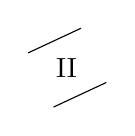
\begin{tikzpicture}[rotate=25]\node[inner sep=1pt] (n) {II};\draw (-.36,.38)--(.38,.38);\draw (-.36,-.38)--(.38,-.38);\end{tikzpicture}}}
\mspage{(89)}
27.3.

45.    The review yesterday of the various ``test notions'',  turning
around test \var{\over[typed]{c}{c}}{c}{typewriter overwriting}{ps_134-4_001-v0001}ategories and test functors,  turned out a lot longer than
expected,  so much so \var{\deleted{as}}{}{deletion}{ps_134-4_001-v0002} to \var{\inserted{have me}}{\hand{have me}}{insertion}{ps_134-4_001-v0003} get a little weary by the end  -  it was clear
though that this ``travail d'intendance'' was necessary,  not only not to
get lost in a morass of closely related and yet definitely distinct noti-%
ons,  but also to gain perspective and a better feeling of the formal struc%
ture of the whole set-up.  As has been the case so often, \var{\over{a}{d}}{\hand{d}}{writing over}{ps_134-4_001-v0004}uring this
\var{\deleted{ungratifying}}{}{deletion}{ps_134-4_001-v0005} \var{\inserted{very}}{\hand{very}}{insertion}{ps_134-4_001-v0006} work of ``grinding through'',  there has appeared \var{\xout{again}}{}{typewriter deletion}{ps_134-4_001-v0007} this
caracteristic feeling of getting close to something ``burning'' again, some-%
thing very simple-minded surely which has kept showing up gradually and
more and more on all odds and ends,  and \var{\inserted[typed]{which}}{which}{typed insertion}{ps_134-4_001-v0008} still is escaping,  still elusive\hand{.}
T$\overset{\hand{\unsure{\wedge}}}{\mathrm{h}}$ere is an impressive bunch of things \var{\deleted{though}}{}{deletion}{ps_134-4_001-v0009} which are demanding pressing%
ly  more or less immediate investigation  -  still I can't help,  I'll
have to try and pin down some way or other this \hand{``}burning spot\hand{''}.

T\var{\over[typed]{H}{h}}{h}{typewriter overwriting}{ps_134-4_001-v0010}ere seem to be recurring striking features of the modelizers met
with so far  -  namely essentially (Cat) and the elementary modelizers $A^{\hand{\wedge}}$
and possibly their ``weak'' variants.  I\var{\over[typed]{N}{n}}{n}{typewriter overwriting}{ps_134-4_001-v0011} all of them,  there is a very
strong interplay between the following notions,  which seem to be the
basic ones and \var{\over{\unsure{m}}{m}}{\hand{m}}{writing over}{ps_134-4_001-v0012}ore or less determine each other mutually:  \uline{weak equiva-}%
\uline{lences} (which define the modelizing structure of the given modelizer M),
\uline{aspheric objects}  (namely such that  $x \hand{\to} e_M$ is a weak equivalence),
\uline{homotopy intervals}  $(I,\hand{\delta}_0,\hand{\delta}_1)$,  and last not least,  the notion of a test
functor  $A \hand{\longrightarrow} M$ ,  where A is a test category (or more generally weak
test functors of weak test categories into M).  The latter so far have
been defined only when M = (Cat),  and initially they were viewed \var{\xout{rather}}{}{typewriter deletion}{ps_134-4_001-v0013}
as being mainly  more handy substitu\var{\over{\unsure{t}}{t}}{\hand{t}}{writing over}{ps_134-4_001-v0014}\var{\over{e}{e}}{\hand{e}}{writing over}{ps_134-4_001-v0015}\var{\over{s}{s}}{\hand{s}}{writing over}{ps_134-4_001-v0016} to \var{\xout{functors}}{}{typewriter deletion}{ps_134-4_001-v0017} $j_A$\hand{,} for getting a
model-preserving functor (Cat)$\hand{\to}$ $A^{\hand{\wedge}}$ quasi-inverse to the all-important
\var{\xout{functor}}{}{typewriter deletion}{ps_134-4_001-v0018} model-preserving functor \var{\xout{\illegible{1}}}{}{typewriter deletion}{ps_134-4_001-v0019}  $i_A : A^{\hand{\wedge}}\hand{\to}$(Cat) ,  $F \hand{\mapsto} A_{\hand{/}F}$ .  I sus-%
pect however that their role is \var{\inserted[typed]{a}}{a}{typed insertion}{ps_134-4_001-v0020} considerably more basic one than just
computational convenience  -  and this reminds me of the analoguous fee-%
ling I had,  when first contemplating using such a thing as (by then still
vaguely conceived) ``test categories'',  for investigating ways of putting
modelizing structures on categories M such as categories of algebraic
structures of some kind or \var{\xout{r}}{}{typewriter deletion}{ps_134-4_001-v0021}\var{\over[typed]{\unsure{a}}{o}}{o}{typewriter overwriting}{ps_134-4_001-v0022}ther. (Cf. notes of march 7,  and more speci-%
fically par. 26  -  this was the very day,  by the way,  I first had th\var{\over{e}{i}}{\hand{i}}{writing over}{ps_134-4_001-v0023}\var{\over{s}{s}}{\hand{s}}{writing over}{ps_134-4_001-v0024}
feeling of being ``burning'' ...)

\margin{1}

%% END SOURCE ps_134-4_001
\ifnum\EditionMode=1
\psapparatusstart
\psentry{ps_134-4_001-v0001}{1}{typewriter overwriting}{\over[typed]{c}{c}}{c}{The superposed typed reading replaces the underlying reading.}
\psentry{ps_134-4_001-v0002}{2}{deletion}{\deleted{as}}{}{The author cancels this material by hand; it leaves the corrected running text.}
\psentry{ps_134-4_001-v0003}{3}{insertion}{\inserted{have me}}{\hand{have me}}{The handwritten insertion is incorporated at its indicated position; insertion brackets leave the running text.}
\psentry{ps_134-4_001-v0004}{4}{writing over}{\over{a}{d}}{\hand{d}}{The superposed handwritten reading replaces the underlying reading.}
\psentry{ps_134-4_001-v0005}{5}{deletion}{\deleted{ungratifying}}{}{The author cancels this material by hand; it leaves the corrected running text.}
\psentry{ps_134-4_001-v0006}{6}{insertion}{\inserted{very}}{\hand{very}}{The handwritten insertion is incorporated at its indicated position; insertion brackets leave the running text.}
\psentry{ps_134-4_001-v0007}{7}{typewriter deletion}{\xout{again}}{}{The typewriter strikes out this material; it leaves the corrected running text.}
\psentry{ps_134-4_001-v0008}{8}{typed insertion}{\inserted[typed]{which}}{which}{The typed insertion is incorporated at its indicated position; insertion brackets leave the running text.}
\psentry{ps_134-4_001-v0009}{9}{deletion}{\deleted{though}}{}{The author cancels this material by hand; it leaves the corrected running text.}
\psentry{ps_134-4_001-v0010}{10}{typewriter overwriting}{\over[typed]{H}{h}}{h}{The superposed typed reading replaces the underlying reading.}
\psentry{ps_134-4_001-v0011}{11}{typewriter overwriting}{\over[typed]{N}{n}}{n}{The superposed typed reading replaces the underlying reading.}
\psentry{ps_134-4_001-v0012}{12}{writing over}{\over{\unsure{m}}{m}}{\hand{m}}{The superposed handwritten reading replaces the underlying reading.}
\psentry{ps_134-4_001-v0013}{13}{typewriter deletion}{\xout{rather}}{}{The typewriter strikes out this material; it leaves the corrected running text.}
\psentry{ps_134-4_001-v0014}{14}{writing over}{\over{\unsure{t}}{t}}{\hand{t}}{The superposed handwritten reading replaces the underlying reading.}
\psentry{ps_134-4_001-v0015}{15}{writing over}{\over{e}{e}}{\hand{e}}{The superposed handwritten reading replaces the underlying reading.}
\psentry{ps_134-4_001-v0016}{16}{writing over}{\over{s}{s}}{\hand{s}}{The superposed handwritten reading replaces the underlying reading.}
\psentry{ps_134-4_001-v0017}{17}{typewriter deletion}{\xout{functors}}{}{The typewriter strikes out this material; it leaves the corrected running text.}
\psentry{ps_134-4_001-v0018}{18}{typewriter deletion}{\xout{functor}}{}{The typewriter strikes out this material; it leaves the corrected running text.}
\psentry{ps_134-4_001-v0019}{19}{typewriter deletion}{\xout{\illegible{1}}}{}{The typewriter strikes out this material; it leaves the corrected running text.}
\psentry{ps_134-4_001-v0020}{20}{typed insertion}{\inserted[typed]{a}}{a}{The typed insertion is incorporated at its indicated position; insertion brackets leave the running text.}
\psentry{ps_134-4_001-v0021}{21}{typewriter deletion}{\xout{r}}{}{The typewriter strikes out this material; it leaves the corrected running text.}
\psentry{ps_134-4_001-v0022}{22}{typewriter overwriting}{\over[typed]{\unsure{a}}{o}}{o}{The superposed typed reading replaces the underlying reading.}
\psentry{ps_134-4_001-v0023}{23}{writing over}{\over{e}{i}}{\hand{i}}{The superposed handwritten reading replaces the underlying reading.}
\psentry{ps_134-4_001-v0024}{24}{writing over}{\over{s}{s}}{\hand{s}}{The superposed handwritten reading replaces the underlying reading.}
\psapparatusend
\fi
\pssource{ps_134-4_002}{134-4/2}{https://grothendieck.umontpellier.fr/web/viewer.html?file=../134-4.pdf\#page=3}
\psnumber{ps_134-4_002-v0001}{1}
\psnumber{ps_134-4_002-v0002}{2}
\psnumber{ps_134-4_002-v0003}{3}
\psnumber{ps_134-4_002-v0004}{4}
\psnumber{ps_134-4_002-v0005}{5}
\psnumber{ps_134-4_002-v0006}{6}
\psnumber{ps_134-4_002-v0007}{7}
\psnumber{ps_134-4_002-v0008}{8}
\psnumber{ps_134-4_002-v0009}{9}
\psnumber{ps_134-4_002-v0010}{10}
%% BEGIN SOURCE ps_134-4_002
% Pursuing Stacks (cotes 134-2 to 134-8): archive cote 134-4, site page 2 (PDF page 3), typescript page 90.
% typescript. Draft compared: ps3.tex:46-112.
% AI-transcribed by Claude Opus 5.5 (claude-opus-5-5, adaptive thinking, effort high), Message Batches API, batch ps1 (msgbatch_01Rv5hCaNTtUt4JHx1yqoHPL), 2026-11-12; image review recorded in records/CHECK_DECISIONS_134_3_4.tsv.
\scanpage{134-4/2}
\mspage{(90)}

Test categories seem to play a similar role here as \var{\inserted[typed]{(the spectra of)}}{(the spectra of)}{typed insertion}{ps_134-4_002-v0001} discrete valuati-%
on rings in algebraic geometry -  they can be mapped into anywhere\hand{,} to
``test'' what is going on there  -  here it means,  they can be sent into
any modelizer (M,W)  (at least among the ones which we feel are the most
interesting) ,  by \var{\xout{functors}}{}{typewriter deletion}{ps_134-4_002-v0002} ``test functors''  $i\colon A\hand{\longrightarrow} M$  giving rise to
a model-preserving functor  $i^{*}$ :  $M\hand{\longrightarrow} A^{\hand{\wedge}}$,  allowing comparison of M with
an elementary modelizer $A^{\hand{\wedge}}$.  As for the all-encompassing basic modelizer
(Cat),  it seems to play the opposite role in a sense,  at least with
respect to elementary modelizers\var{\xout{\unsure{,}}}{}{typewriter deletion}{ps_134-4_002-v0003} $A^{\hand{\wedge}}$,  which all admit modelizing maps
$i_A$ :  $A^{\hand{\wedge}}\hand{\longrightarrow}$(Cat).  As a matter of fact,  for given \var{\over{t}{t}}{\hand{t}}{writing over}{ps_134-4_002-v0004}est category A i.e.
a given elementary modelizer $A^{\hand{\wedge}}$,  I see for the time being just \uline{one} way
to get a modelizing functor from it to (Cat),  namely just the canonical
$i_A$ .  T\var{\over[typed]{H}{h}}{h}{typewriter overwriting}{ps_134-4_002-v0005}ere is also a striking difference between the exactness properties
of the functors
\[ \text{(1)}\qquad i^{*} : M\hand{\longrightarrow} A^{\hand{\wedge}} \]
one way,  which commute to inverse limits,  and the functors
\[ \text{(2)}\qquad i_A\colon A^{\hand{\wedge}}\hand{\longrightarrow}\text{(Cat)} \]
in the other direction,  commuting to direct limits.  Another difference
is that we should not expect that the left adjoint  $i_{\hand{!}}$ to $i^{*}$ be model pre-%
serving too (with the exception of the very special case when M=(Cat) and
$i\colon A\hand{\longrightarrow} M$ = (Cat)  is the canonical functor $i_A$ ,  which appears as highly
non typical in this respect ),  whereas the right adjoint  $j_A=i_A^{\,*}$  of $i_A$
is model preserving,  thus $i_A$ is part of a pair $(i_A,j_A)$ of model preser-%
ving adjoint functors.

Of course,  we may want to compare \var{\inserted[typed]{directly}}{directly}{typed insertion}{ps_134-4_002-v0006} \unsure{an} arbitrary modelizer M to (Cat)
by sending it into (Cat) by a modelizing functor  $M\hand{\longrightarrow}$(Cat);  we get quite
naturally such a functor \hand{(for any given choice of test-functor $i\colon A\to M$)}
\[ \text{(3)}\qquad i_Ai^{*} :\ M\hand{\longrightarrow}\text{(Cat)}\quad , \]
but this functor is not likely any more to commute \var{\deleted{to}}{}{deletion}{ps_134-4_002-v0007} neither \var{\inserted{to}}{\hand{to}}{insertion}{ps_134-4_002-v0008} direct nor\hand{ to}
inverse limits, even finite ones  -  and it is\hand{'}n\var{\over{t}{t}}{\hand{t}}{writing over}{ps_134-4_002-v0009} too clear that for a
modelizer M which is'nt elementary,  we have much chance to get a modeli-%
zing functor to (Cat) which is either left or right exact.  However,  the
functors \var{\inserted{(3)}}{\hand{(3)}}{insertion}{ps_134-4_002-v0010} we've got,  whenever modelizing and if M is a \uline{strict} modelizer
(namely $M\hand{\longrightarrow} W_M^{-1}M\hand{\simeq}$(Hot)  commutes with finite products),  will commute
to finite products ``up to weak equivalence''.  Also the functors $i^{*}$ ,  al-%
though not right exact definitely,  have a tendency to commute to sums,\margin{also to fibered products $\times$}
and hence the same will hold (not only up to weak equivalence) for (3).

As for getting a modelizing functor  (Cat)$\hand{\longrightarrow}$M ,  for a modelizer M

\margin{2}

%% END SOURCE ps_134-4_002
\ifnum\EditionMode=1
\psapparatusstart
\psentry{ps_134-4_002-v0001}{1}{typed insertion}{\inserted[typed]{(the spectra of)}}{(the spectra of)}{The typed insertion is incorporated at its indicated position; insertion brackets leave the running text.}
\psentry{ps_134-4_002-v0002}{2}{typewriter deletion}{\xout{functors}}{}{The typewriter strikes out this material; it leaves the corrected running text.}
\psentry{ps_134-4_002-v0003}{3}{typewriter deletion}{\xout{\unsure{,}}}{}{The typewriter strikes out this material; it leaves the corrected running text.}
\psentry{ps_134-4_002-v0004}{4}{writing over}{\over{t}{t}}{\hand{t}}{The superposed handwritten reading replaces the underlying reading.}
\psentry{ps_134-4_002-v0005}{5}{typewriter overwriting}{\over[typed]{H}{h}}{h}{The superposed typed reading replaces the underlying reading.}
\psentry{ps_134-4_002-v0006}{6}{typed insertion}{\inserted[typed]{directly}}{directly}{The typed insertion is incorporated at its indicated position; insertion brackets leave the running text.}
\psentry{ps_134-4_002-v0007}{7}{deletion}{\deleted{to}}{}{The author cancels this material by hand; it leaves the corrected running text.}
\psentry{ps_134-4_002-v0008}{8}{insertion}{\inserted{to}}{\hand{to}}{The handwritten insertion is incorporated at its indicated position; insertion brackets leave the running text.}
\psentry{ps_134-4_002-v0009}{9}{writing over}{\over{t}{t}}{\hand{t}}{The superposed handwritten reading replaces the underlying reading.}
\psentry{ps_134-4_002-v0010}{10}{insertion}{\inserted{(3)}}{\hand{(3)}}{The handwritten insertion is incorporated at its indicated position; insertion brackets leave the running text.}
\psapparatusend
\fi
\pssource{ps_134-4_003}{134-4/3}{https://grothendieck.umontpellier.fr/web/viewer.html?file=../134-4.pdf\#page=4}
\psnumber{ps_134-4_003-v0001}{1}
\psnumber{ps_134-4_003-v0002}{2}
\psnumber{ps_134-4_003-v0003}{3}
\psnumber{ps_134-4_003-v0004}{4}
\psnumber{ps_134-4_003-v0005}{5}
\psnumber{ps_134-4_003-v0006}{6}
\psnumber{ps_134-4_003-v0007}{7}
\psnumber{ps_134-4_003-v0008}{8}
\psnumber{ps_134-4_003-v0009}{9}
\psnumber{ps_134-4_003-v0010}{10}
\psnumber{ps_134-4_003-v0011}{11}
\psnumber{ps_134-4_003-v0012}{12}
\psnumber{ps_134-4_003-v0013}{13}
\psnumber{ps_134-4_003-v0014}{14}
\psnumber{ps_134-4_003-v0015}{15}
\psnumber{ps_134-4_003-v0016}{16}
\psnumber{ps_134-4_003-v0017}{17}
\psnumber{ps_134-4_003-v0018}{18}
\psnumber{ps_134-4_003-v0019}{19}
\psnumber{ps_134-4_003-v0020}{20}
\psnumber{ps_134-4_003-v0021}{21}
\psnumber{ps_134-4_003-v0022}{22}
\psnumber{ps_134-4_003-v0023}{23}
\psnumber{ps_134-4_003-v0024}{24}
\psnumber{ps_134-4_003-v0025}{25}
\psnumber{ps_134-4_003-v0026}{26}
\psnumber{ps_134-4_003-v0027}{27}
%% BEGIN SOURCE ps_134-4_003
% Pursuing Stacks (cotes 134-2 to 134-8): archive cote 134-4, site page 3 (PDF page 4), typescript page 91.
% typescript. Draft compared: ps3.tex:99-179.
% AI-transcribed by Claude Opus 5.5 (claude-opus-5-5, adaptive thinking, effort high), Message Batches API, batch ps1 (msgbatch_01Rv5hCaNTtUt4JHx1yqoHPL), 2026-11-12; image review recorded in records/CHECK_DECISIONS_134_3_4.tsv.
\scanpage{134-4/3}
\mspage{(91)}
which is'nt elementary,  in view of having a standart way for describing
a given homotopy type (defined by an object $C$ in (Cat)) by a``model'' in $M$
depending functorially on $C$,  there does'nt seem to be any general process
for finding one,  even without any demand on exactness properties,  ex\var{\over[typed]{c}{c}}{c}{typewriter overwriting}{ps_134-4_003-v0001}\var{\over[typed]{e}{e}}{e}{typewriter overwriting}{ps_134-4_003-v0002}pt
of course when $M$ is supposed to be elementary;   in this ca\var{\over[typed]{s}{s}}{s}{typewriter overwriting}{ps_134-4_003-v0003}e \var{\xout{xx}}{}{typewriter deletion}{ps_134-4_003-v0004} $M = A^{\hand{\wedge}}$
we get \var{\xout{of course}}{}{typewriter deletion}{ps_134-4_003-v0005} the functors
\[ (4) \qquad i^* : (\mathrm{Cat}) \hand{\longrightarrow} \var{\over[typed]{A}{A}}{A}{typewriter overwriting}{ps_134-4_003-v0006}^{\hand{\wedge}} \]
associated to test functors $A \hand{\to} (\mathrm{Cat})$,  which can be viewed as a particula\unsure{r}
case of (1),  applied to the case $M = (\mathrm{Cat})$.  Using \var{\xout{this}}{}{typewriter deletion}{ps_134-4_003-v0007} such functors
(4),  we see that the question of finding a modelizing functor
\[ (*) \qquad \hand{\phi} : (\mathrm{Cat}) \hand{\longrightarrow} M \ , \]
for a more or less general $M$,  is tied up with the question of finding
such a functor from an elementary modelizer $A^{\hand{\wedge}}$ into $M$
\[ (**) \qquad \hand{\psi} : A^{\hand{\wedge}} \hand{\longrightarrow} M \ , \]
M\var{\over[typed]{o}{o}}{o}{typewriter overwriting}{ps_134-4_003-v0008}re specifically,  if we got a $\hand{\psi}$ ,  we deduce a $\hand{\phi}$ by composing with
$i^*$ in (4) ,  and conversely,  if we got a $\hand{\phi}$ ,  we deduce a $\hand{\psi}$ by composing
with the canonical functor $i_A$ in (2).  Maybe it's unrealistic to expect
modelizing functors (*) or (**) to exist for rather general M. (\var{\over{w}{W}}{\hand{W}}{writing over}{ps_134-4_003-v0009}hich \var{\xout{ones}}{}{typewriter deletion}{ps_134-4_003-v0010} \var{\inserted[typed]{modelizers}}{modelizers}{typed insertion}{ps_134-4_003-v0011}
will turn out to be really ``the interesting ones'' will appear in due \var{\over{\unsure{c}}{c}}{\hand{c}}{writing over}{ps_134-4_003-v0012}our-%
se presumably...).  T\var{\over[typed]{h}{h}}{h}{typewriter overwriting}{ps_134-4_003-v0013}ere is  one interesting case though when we got such
functors,  namely when
\[ M = (\mathrm{Spaces}) \]
is the category of topological spaces, \var{\inserted{and}}{\hand{and}}{insertion}{ps_134-4_003-v0014} taking for $\hand{\psi}$ one of the manifold
\var{\xout{species}}{}{typewriter deletion}{ps_134-4_003-v0015} \var{\inserted[typed]{avators}}{avators}{typed insertion}{ps_134-4_003-v0016} of ``geometric realization functor'' ,  associated to a \var{\inserted{suitable}}{\hand{suitable}}{insertion}{ps_134-4_003-v0017} functor
\[ \var{\xout{(5)}}{}{typewriter deletion}{ps_134-4_003-v0018} \qquad r : A \hand{\longrightarrow} (\mathrm{Spaces}) \]
by taking the canonical extension $r_{\hand{!}}$ to $A^{\hand{\wedge}}$,  commuting with direct limits\unsure{.}
This is presisely the \var{\xout{case}}{}{typewriter deletion}{ps_134-4_003-v0019} ``highly non typical'' case,  when we get a
pair of adjoint functors  $r_{\hand{!}}$ , $r^*$
% Hand-drawn arrows are marked blue; typed objects remain plain.
\noindent $(5)\qquad$ \diagram{\begin{tikzcd} A^{\hand{\wedge}} \ar[r, shift left,color=blue, "\hand{r_!}"] \& (\mathrm{Spaces}) \ar[l, shift left,color=blue, "\hand{r^*}"] \end{tikzcd}}
which are \uline{both} modelizing.  T\var{\over[typed]{H}{h}}{h}{typewriter overwriting}{ps_134-4_003-v0020}e situation  here mimicks very closely the
situation of the pair $(i_A, j_A = i_A^* )$ canonically associated to the elementa-%
r\var{\over[typed]{u}{y}}{y}{typewriter overwriting}{ps_134-4_003-v0021} modelizer $A^{\hand{\wedge}}$,  with the ``basic modelizer'' (Cat)  being replaced by
(Spaces),  which therefore can be consid\var{\over[typed]{\illegible{1}}{e}}{e}{typewriter overwriting}{ps_134-4_003-v0022}red  as another ``basic modelizer''
of sorts.  In this case  the corresponding functor
\[ \var{\xout{(xxxx)}}{}{typewriter deletion}{ps_134-4_003-v0023} \ (6) \qquad r_{\hand{!}} i^* : (\mathrm{Cat}) \hand{\longrightarrow} (\var{\over[typed]{\mathrm{Spa}}{\mathrm{Spa}}}{\mathrm{Spa}}{typewriter overwriting}{ps_134-4_003-v0024}\var{\over{\mathrm{c}}{\mathrm{c}}}{\hand{\mathrm{c}}}{writing over}{ps_134-4_003-v0025}\mathrm{es}) \]
mimicks  the functor  $i_A i^*$ of (3) (where on the left hand side $M$ is
taken to be just (Cat),  and on the right (Cat) as the basic modelizer is
replaced by \var{\over[typed]{it}{it}}{it}{typewriter overwriting}{ps_134-4_003-v0026}'s \hand{``}next best\hand{''} substitu\var{\over[typed]{e}{t}}{t}{typewriter overwriting}{ps_134-4_003-v0027}e (Spaces)).   Here as in (3),  the
modelizing functor we got is neither left nor right exact,  it has a ten-%

\margin{3}

%% END SOURCE ps_134-4_003
\ifnum\EditionMode=1
\psapparatusstart
\psentry{ps_134-4_003-v0001}{1}{typewriter overwriting}{\over[typed]{c}{c}}{c}{The superposed typed reading replaces the underlying reading.}
\psentry{ps_134-4_003-v0002}{2}{typewriter overwriting}{\over[typed]{e}{e}}{e}{The superposed typed reading replaces the underlying reading.}
\psentry{ps_134-4_003-v0003}{3}{typewriter overwriting}{\over[typed]{s}{s}}{s}{The superposed typed reading replaces the underlying reading.}
\psentry{ps_134-4_003-v0004}{4}{typewriter deletion}{\xout{xx}}{}{The typewriter strikes out this material; it leaves the corrected running text.}
\psentry{ps_134-4_003-v0005}{5}{typewriter deletion}{\xout{of course}}{}{The typewriter strikes out this material; it leaves the corrected running text.}
\psentry{ps_134-4_003-v0006}{6}{typewriter overwriting}{$\over[typed]{A}{A}$}{$A$}{The superposed typed reading replaces the underlying reading.}
\psentry{ps_134-4_003-v0007}{7}{typewriter deletion}{\xout{this}}{}{The typewriter strikes out this material; it leaves the corrected running text.}
\psentry{ps_134-4_003-v0008}{8}{typewriter overwriting}{\over[typed]{o}{o}}{o}{The superposed typed reading replaces the underlying reading.}
\psentry{ps_134-4_003-v0009}{9}{writing over}{\over{w}{W}}{\hand{W}}{The superposed handwritten reading replaces the underlying reading.}
\psentry{ps_134-4_003-v0010}{10}{typewriter deletion}{\xout{ones}}{}{The typewriter strikes out this material; it leaves the corrected running text.}
\psentry{ps_134-4_003-v0011}{11}{typed insertion}{\inserted[typed]{modelizers}}{modelizers}{The typed insertion is incorporated at its indicated position; insertion brackets leave the running text.}
\psentry{ps_134-4_003-v0012}{12}{writing over}{\over{\unsure{c}}{c}}{\hand{c}}{The superposed handwritten reading replaces the underlying reading.}
\psentry{ps_134-4_003-v0013}{13}{typewriter overwriting}{\over[typed]{h}{h}}{h}{The superposed typed reading replaces the underlying reading.}
\psentry{ps_134-4_003-v0014}{14}{insertion}{\inserted{and}}{\hand{and}}{The handwritten insertion is incorporated at its indicated position; insertion brackets leave the running text.}
\psentry{ps_134-4_003-v0015}{15}{typewriter deletion}{\xout{species}}{}{The typewriter strikes out this material; it leaves the corrected running text.}
\psentry{ps_134-4_003-v0016}{16}{typed insertion}{\inserted[typed]{avators}}{avators}{The typed insertion is incorporated at its indicated position; insertion brackets leave the running text.}
\psentry{ps_134-4_003-v0017}{17}{insertion}{\inserted{suitable}}{\hand{suitable}}{The handwritten insertion is incorporated at its indicated position; insertion brackets leave the running text.}
\psentry{ps_134-4_003-v0018}{18}{typewriter deletion}{$\xout{(5)}$}{}{The typewriter strikes out this material; it leaves the corrected running text.}
\psentry{ps_134-4_003-v0019}{19}{typewriter deletion}{\xout{case}}{}{The typewriter strikes out this material; it leaves the corrected running text.}
\psentry{ps_134-4_003-v0020}{20}{typewriter overwriting}{\over[typed]{H}{h}}{h}{The superposed typed reading replaces the underlying reading.}
\psentry{ps_134-4_003-v0021}{21}{typewriter overwriting}{\over[typed]{u}{y}}{y}{The superposed typed reading replaces the underlying reading.}
\psentry{ps_134-4_003-v0022}{22}{typewriter overwriting}{\over[typed]{\illegible{1}}{e}}{e}{The superposed typed reading replaces the underlying reading.}
\psentry{ps_134-4_003-v0023}{23}{typewriter deletion}{$\xout{(xxxx)}$}{}{The typewriter strikes out this material; it leaves the corrected running text.}
\psentry{ps_134-4_003-v0024}{24}{typewriter overwriting}{$\over[typed]{\mathrm{Spa}}{\mathrm{Spa}}$}{$\mathrm{Spa}$}{The superposed typed reading replaces the underlying reading.}
\psentry{ps_134-4_003-v0025}{25}{writing over}{$\over{\mathrm{c}}{\mathrm{c}}$}{$\hand{\mathrm{c}}$}{The superposed handwritten reading replaces the underlying reading.}
\psentry{ps_134-4_003-v0026}{26}{typewriter overwriting}{\over[typed]{it}{it}}{it}{The superposed typed reading replaces the underlying reading.}
\psentry{ps_134-4_003-v0027}{27}{typewriter overwriting}{\over[typed]{e}{t}}{t}{The superposed typed reading replaces the underlying reading.}
\psapparatusend
\fi
\pssource{ps_134-4_004}{134-4/4}{https://grothendieck.umontpellier.fr/web/viewer.html?file=../134-4.pdf\#page=5}
\psnumber{ps_134-4_004-v0001}{1}
\psnumber{ps_134-4_004-v0002}{2}
\psnumber{ps_134-4_004-v0003}{3}
\psnumber{ps_134-4_004-v0004}{4}
\psnumber{ps_134-4_004-v0005}{5}
\psnumber{ps_134-4_004-v0006}{6}
\psnumber{ps_134-4_004-v0007}{7}
\psnumber{ps_134-4_004-v0008}{8}
\psnumber{ps_134-4_004-v0009}{9}
\psnumber{ps_134-4_004-v0010}{10}
\psnumber{ps_134-4_004-v0011}{11}
\psnumber{ps_134-4_004-v0012}{12}
\psnumber{ps_134-4_004-v0013}{13}
\psnumber{ps_134-4_004-v0014}{14}
\psnumber{ps_134-4_004-v0015}{15}
\psnumber{ps_134-4_004-v0016}{16}
\psnumber{ps_134-4_004-v0017}{17}
\psnumber{ps_134-4_004-v0018}{18}
\psnumber{ps_134-4_004-v0019}{19}
\psnumber{ps_134-4_004-v0020}{20}
\psnumber{ps_134-4_004-v0021}{21}
%% BEGIN SOURCE ps_134-4_004
% Pursuing Stacks (cotes 134-2 to 134-8): archive cote 134-4, site page 4 (PDF page 5), typescript page 92.
% typescript. Draft compared: ps3.tex:161-221.
% AI-transcribed by Claude Opus 5.5 (claude-opus-5-5, adaptive thinking, effort high), Message Batches API, batch ps1 (msgbatch_01Rv5hCaNTtUt4JHx1yqoHPL), 2026-11-12; image review recorded in records/CHECK_DECISIONS_134_3_4.tsv.
\scanpage{134-4/4}
\var{\xout{(92)}}{}{typewriter deletion}{ps_134-4_004-v0001}
\mspage{(92)}
dency though to commute to sums,  as usual.

I would'nt overemphasize the capacity of (Spaces\var{\over{'}{)}}{\hand{)}}{writing over}{ps_134-4_004-v0002} to serve the purpose
of a ``basic modelizer'' as \var{\inserted{does}}{\hand{does}}{insertion}{ps_134-4_004-v0003} (Cat),  despite the attractive feature of more
direct (or at any rate,  more convential) ties with so-called ``topological
intuition''.  O\var{\over[typed]{N}{n}}{n}{typewriter overwriting}{ps_134-4_004-v0004}e drawback of (Spaces) is the relative sophistication of
the structure species ``topological spaces'' it corresponds to,  which is
by no means an ``algebraic structure species'',  and fits into algebraic
formalism\hand{s} only at the price of detours.  M$\overset{\hand{\smile}}{\mathrm{o}}$re seriously still,  or rather
as a reflection of this latter feature,  only for some rather special
elementary modelizers $A^{\hand{\wedge}}$,  namely rather special test categories $A$,  do
we get a geometric realization functor $r_{\hand{!}} : A^{\hand{\wedge}} \hand{\longrightarrow} (\mathrm{Spaces})$ which \var{\over[typed]{i}{c}}{c}{typewriter overwriting}{ps_134-4_004-v0005}\var{\over[typed]{a}{a}}{a}{typewriter overwriting}{ps_134-4_004-v0006}n be
viewed as part of a pair of mutually adjoint modelizing functors,
mimicking the \var{\over[typed]{p}{c}}{c}{typewriter overwriting}{ps_134-4_004-v0007}anonical pair $(i_A, j_A)$;  still \var{\over{t}{l}}{\hand{l}}{writing over}{ps_134-4_004-v0008}\var{\over{e}{e}}{\hand{e}}{writing over}{ps_134-4_004-v0009}ss \var{\over[typed]{d}{d}}{d}{typewriter overwriting}{ps_134-4_004-v0010}oes there seem\var{\deleted{s}}{}{deletion}{ps_134-4_004-v0011} to be
anything like a really canonical choice (although some choices are pretty
natural indeed,  dealing with the standart test categories such as \hand{$\Delta$} and
it\hand{'}s variants).  At any rate,  it is still to be seen whether there exists
such a pair  $(r_{\hand{!}}, r^{*})$  for \hand{some} rather general class\var{\deleted{\unsure{e}}}{}{deletion}{ps_134-4_004-v0012} of test categories  -
this is one among the very many things that I keep pushing off,  as more
urgent matters are calling for attention ...

To sum up the outcome of these unformal reflections \var{\deleted{upon}}{}{deletion}{ps_134-4_004-v0013} \var{\inserted{about}}{\hand{about}}{insertion}{ps_134-4_004-v0014} various
types of modelizing functors between modelizers,  the two main types which
seem to overtower the whole picture,  and are likely to be the essential
ones for a general understanding of homotopy models,  are the two types
(1) and (2)  above.  T\var{\over[typed]{H}{h}}{h}{typewriter overwriting}{ps_134-4_004-v0015}e first one $i^{*}$ is defined in terms of an arbitrary
test functor (still to be \var{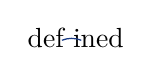
\begin{tikzpicture}[baseline=(w.base)]\node[inner sep=0pt] (w) {def ined};\draw[color=blue,line width=.45pt] ([xshift=-.5em,yshift=.65ex]w.south) to[bend left=20] ([xshift=.2em,yshift=.65ex]w.south);\end{tikzpicture}}{defined}{authorial word join}{ps_134-4_004-v0016} !)  of a test category into an arbitra-%
ry\var{\xout{x}}{}{typewriter deletion}{ps_134-4_004-v0017} modelizer $M$.  The second $i_A$ ,  with opposite exactness properties to
the previous one,  is canonically attached to any test category,  and
\var{\xout{ties}}{}{typewriter deletion}{ps_134-4_004-v0018} maps the corresponding elementary modelizer  $A^{\hand{\wedge}}$ into the basic mode-%
lizer (Cat),  without any reference to more general types of modelizers $M$.
The right adjoint of the latter,  which is still model preserving,  is
in fact of the type (1) again,  for the canonical test functor $A \hand{\longrightarrow} (\mathrm{Cat})$
induced by $i_A$ ,  namely $a \hand{\mapsto} A_{\hand{/}a}$ .  \var{\begin{tikzpicture}[baseline=-.2ex]\draw[color=blue] (0,0)--(.45,0)--(.45,.4)--(.82,.4);\draw[color=blue] (.49,.02)--(.49,.42);\end{tikzpicture}}{

}{authorial paragraph break}{ps_134-4_004-v0019} T\var{\over[typed]{H}{h}}{h}{typewriter overwriting}{ps_134-4_004-v0020}\var{\over{e}{is}}{\hand{is}}{writing over}{ps_134-4_004-v0021} whole reflection was of course on
such an unformal level,  that there was no sense at that stage to bother
with distinctions between weaker or stricter  variants of the test-notions
Maybe it's about time now to start getting a little more specific.

\margin{4}

%% END SOURCE ps_134-4_004
\ifnum\EditionMode=1
\psapparatusstart
\psentry{ps_134-4_004-v0001}{1}{typewriter deletion}{\xout{(92)}}{}{The typewriter strikes out this material; it leaves the corrected running text.}
\psentry{ps_134-4_004-v0002}{2}{writing over}{\over{'}{)}}{\hand{)}}{The superposed handwritten reading replaces the underlying reading.}
\psentry{ps_134-4_004-v0003}{3}{insertion}{\inserted{does}}{\hand{does}}{The handwritten insertion is incorporated at its indicated position; insertion brackets leave the running text.}
\psentry{ps_134-4_004-v0004}{4}{typewriter overwriting}{\over[typed]{N}{n}}{n}{The superposed typed reading replaces the underlying reading.}
\psentry{ps_134-4_004-v0005}{5}{typewriter overwriting}{\over[typed]{i}{c}}{c}{The superposed typed reading replaces the underlying reading.}
\psentry{ps_134-4_004-v0006}{6}{typewriter overwriting}{\over[typed]{a}{a}}{a}{The superposed typed reading replaces the underlying reading.}
\psentry{ps_134-4_004-v0007}{7}{typewriter overwriting}{\over[typed]{p}{c}}{c}{The superposed typed reading replaces the underlying reading.}
\psentry{ps_134-4_004-v0008}{8}{writing over}{\over{t}{l}}{\hand{l}}{The superposed handwritten reading replaces the underlying reading.}
\psentry{ps_134-4_004-v0009}{9}{writing over}{\over{e}{e}}{\hand{e}}{The superposed handwritten reading replaces the underlying reading.}
\psentry{ps_134-4_004-v0010}{10}{typewriter overwriting}{\over[typed]{d}{d}}{d}{The superposed typed reading replaces the underlying reading.}
\psentry{ps_134-4_004-v0011}{11}{deletion}{\deleted{s}}{}{The author cancels this material by hand; it leaves the corrected running text.}
\psentry{ps_134-4_004-v0012}{12}{deletion}{\deleted{\unsure{e}}}{}{The author cancels this material by hand; it leaves the corrected running text.}
\psentry{ps_134-4_004-v0013}{13}{deletion}{\deleted{upon}}{}{The author cancels this material by hand; it leaves the corrected running text.}
\psentry{ps_134-4_004-v0014}{14}{insertion}{\inserted{about}}{\hand{about}}{The handwritten insertion is incorporated at its indicated position; insertion brackets leave the running text.}
\psentry{ps_134-4_004-v0015}{15}{typewriter overwriting}{\over[typed]{H}{h}}{h}{The superposed typed reading replaces the underlying reading.}
\psentry{ps_134-4_004-v0016}{16}{authorial word join}{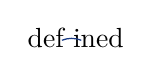
\begin{tikzpicture}[baseline=(w.base)]\node[inner sep=0pt] (w) {def ined};\draw[color=blue,line width=.45pt] ([xshift=-.5em,yshift=.65ex]w.south) to[bend left=20] ([xshift=.2em,yshift=.65ex]w.south);\end{tikzpicture}}{defined}{The pen curve joins the typed def and ined across their internal blank.}
\psentry{ps_134-4_004-v0017}{17}{typewriter deletion}{\xout{x}}{}{The typewriter strikes out this material; it leaves the corrected running text.}
\psentry{ps_134-4_004-v0018}{18}{typewriter deletion}{\xout{ties}}{}{The typewriter strikes out this material; it leaves the corrected running text.}
\psentry{ps_134-4_004-v0019}{19}{authorial paragraph break}{\begin{tikzpicture}[baseline=-.2ex]\draw[color=blue] (0,0)--(.45,0)--(.45,.4)--(.82,.4);\draw[color=blue] (.49,.02)--(.49,.42);\end{tikzpicture}}{

}{The stepped pen mark before This calls for a new paragraph.}
\psentry{ps_134-4_004-v0020}{20}{typewriter overwriting}{\over[typed]{H}{h}}{h}{The superposed typed reading replaces the underlying reading.}
\psentry{ps_134-4_004-v0021}{21}{writing over}{\over{e}{is}}{\hand{is}}{The superposed handwritten reading replaces the underlying reading.}
\psapparatusend
\fi
\pssource{ps_134-4_005}{134-4/5}{https://grothendieck.umontpellier.fr/web/viewer.html?file=../134-4.pdf\#page=6}
\psnumber{ps_134-4_005-v0001}{1}
\psnumber{ps_134-4_005-v0002}{2}
\psnumber{ps_134-4_005-v0003}{3}
\psnumber{ps_134-4_005-v0004}{4}
\psnumber{ps_134-4_005-v0005}{5}
\psnumber{ps_134-4_005-v0006}{6}
\psnumber{ps_134-4_005-v0007}{7}
\psnumber{ps_134-4_005-v0008}{8}
\psnumber{ps_134-4_005-v0009}{9}
\psnumber{ps_134-4_005-v0010}{10}
\psnumber{ps_134-4_005-v0011}{11}
\psnumber{ps_134-4_005-v0012}{12}
\psnumber{ps_134-4_005-v0013}{13}
\psnumber{ps_134-4_005-v0014}{14}
\psnumber{ps_134-4_005-v0015}{15}
\psnumber{ps_134-4_005-v0016}{16}
\psnumber{ps_134-4_005-v0017}{17}
\psnumber{ps_134-4_005-v0018}{18}
\psnumber{ps_134-4_005-v0019}{19}
\psnumber{ps_134-4_005-v0020}{20}
%% BEGIN SOURCE ps_134-4_005
% Pursuing Stacks (cotes 134-2 to 134-8): archive cote 134-4, site page 5 (PDF page 6), typescript page 93.
% typescript. Draft compared: ps3.tex:205-276.
% AI-transcribed by Claude Opus 5.5 (claude-opus-5-5, adaptive thinking, effort high), Message Batches API, batch ps1 (msgbatch_01Rv5hCaNTtUt4JHx1yqoHPL), 2026-11-12; image review recorded in records/CHECK_DECISIONS_134_3_4.tsv.
\scanpage{134-4/5}
\mspage{(93)}
46.   F\unsure{\var{\over[typed]{!}{i}}{i}{typewriter overwriting}{ps_134-4_005-v0001}}rst thing to do visibly is to define  the notion of a test-func\var{\over[typed]{g}{t}}{t}{typewriter overwriting}{ps_134-4_005-v0002}or
\[ i : A^{\unsure{\overset{\hand{/}}{\mathrm{x}}}} \hand{\longrightarrow} M \quad , \]
where M is any modelizer. \var{\deleted{t}}{}{deletion}{ps_134-4_005-v0003}Thus M is endowed with a \var{\xout{famil}}{}{typewriter deletion}{ps_134-4_005-v0004} subset $W_M < \mathrm{F}\unsure{\var{\over{l}{l}}{\hand{l}}{writing over}{ps_134-4_005-v0005}}(M)$
\var{\xout{of}}{}{typewriter deletion}{ps_134-4_005-v0006} \var{i?e. a notion}{i.e. a notion}{slip corrected}{ps_134-4_005-v0007} of weak equivalence,  satisfying the ``mild saturation
conditions'' of p.59,  and moreover we assume that $W_M^{-1}M$  is equivalent to
(Hot)  -  but the choice of an equivalence,  or equivalently,  of the
corresponding localization functor
\[ M \hand{\longrightarrow} (\mathrm{Hot}) \ , \]
is not given with the structure.  (If we admit the ``inspiring assumption'',
there is no real choice,  as a matter of fact  -  but we don't want to use
this in a \var{
\begin{tikzpicture}[baseline=(w.base)]\node[inner sep=0pt] (w) {technic al};\draw[color=blue,line width=.45pt] ([xshift=.65em,yshift=.3ex]w.south) to[bend right=15] ([xshift=1.35em,yshift=.3ex]w.south);\end{tikzpicture}}{technical}{authorial word join}{ps_134-4_005-v0008}  sense,  but only as a guide and motivation.)

Let's start with the weak variant  -  we assume A to be a weak test
category,  and want to define what it means that i is a \uline{weak test functor}.
In all this game,  it is understood that in case M = (Cat),  the notions
we want to define (of a weak test functor and of a test functor) should
\var{beduce to the ones}{reduce to the ones}{slip corrected}{ps_134-4_005-v0009} we have pinpointed in yesterday's notes.

T\var{\over[typed]{H}{h}}{h}{typewriter overwriting}{ps_134-4_005-v0010}e very first idea that comes to mind,  is to demand merely that
the corresponding \var{\xout{it}}{}{typewriter deletion}{ps_134-4_005-v0011} $i^*$  (1)
\[ i^*:\ M \hand{\longrightarrow} A^{\hand{\wedge}} \]
should be  modelizing;$^{\mathrm{x}}$  which means (I recall)
\[ \text{a)}\quad W_M = i^{*\,-1}(W_A\var{\over{)}{)}}{\hand{)}}{writing over}{ps_134-4_005-v0012} \]
\[ \text{b)}\quad \text{The induced functor } W_M^{-1}M \hand{\longrightarrow} W_A^{-1}A^{\hand{\wedge}} \text{ is an equivalence.} \]
This,  I just checked,  does correspond to the definition we gave yester-%
day (p.85),  when  M = (Cat).  T\var{\over[typed]{H}{h}}{h}{typewriter overwriting}{ps_134-4_005-v0013}ere is a very interesting extra feature
though in this special case,  which appears kind of ``in between the lines''
in the ``key result'' on p.61 , \var{\inserted{and}}{\hand{and}}{insertion}{ps_134-4_005-v0014} which I want \var{\inserted{now}}{\hand{now}}{insertion}{ps_134-4_005-v0015} to state in the more general
set up.

As usual in related situations,  the notion of weak equivalence in
M  gives rise to a corresponding notion of ``aspheric'' elements in M -
namely those for which the unique map
\[ x \hand{\longrightarrow} e_M \]
is a weak equivalence. \var{\deleted{w}}{}{deletion}{ps_134-4_005-v0016}We assume now the existence of a final object $e_M$
in M ,  and will assume too,  if necessary,  that it's image in the
localization $W_M^{-1}M$ \var{\inserted[typed]{$= H_M$}}{$= H_M$}{typed insertion}{ps_134-4_005-v0017} is equally a final object.\hand{$*$} \var{\xout{If we assume}}{}{typewriter deletion}{ps_134-4_005-v0018} Thus \var{\inserted[typed]{if}}{if}{typed insertion}{ps_134-4_005-v0019} x in M
is aspheric,  it's image in $H_M$  is a final object,  and the converse holds
provided we assume $W_M$  strongly saturated\hand{,} namely any map in M which becomes
an isomorphism in $H_M$  is a weak equivalence.
\var{\margin{$*$ 29.3. This condition will \inserted{be} verified, if there exists a weak test functor $i:A\to M$.}}{\margin{$*$ 29.3. This condition will \hand{be} verified, if there exists a weak test functor $i:A\to M$.}}{marginal note revised}{ps_134-4_005-v0020}

\margin{5}

%% END SOURCE ps_134-4_005
\ifnum\EditionMode=1
\psapparatusstart
\psentry{ps_134-4_005-v0001}{1}{typewriter overwriting}{\over[typed]{!}{i}}{i}{The superposed typed reading replaces the underlying reading.}
\psentry{ps_134-4_005-v0002}{2}{typewriter overwriting}{\over[typed]{g}{t}}{t}{The superposed typed reading replaces the underlying reading.}
\psentry{ps_134-4_005-v0003}{3}{deletion}{\deleted{t}}{}{The author cancels this material by hand; it leaves the corrected running text.}
\psentry{ps_134-4_005-v0004}{4}{typewriter deletion}{\xout{famil}}{}{The typewriter strikes out this material; it leaves the corrected running text.}
\psentry{ps_134-4_005-v0005}{5}{writing over}{$\over{l}{l}$}{$\hand{l}$}{The superposed handwritten reading replaces the underlying reading.}
\psentry{ps_134-4_005-v0006}{6}{typewriter deletion}{\xout{of}}{}{The typewriter strikes out this material; it leaves the corrected running text.}
\psentry{ps_134-4_005-v0007}{7}{slip corrected}{i?e. a notion}{i.e. a notion}{The question mark is an isolated wrong keystroke in i.e., whose normal form is repeatedly attested in checked pages including 134-3/87.}
\psentry{ps_134-4_005-v0008}{8}{authorial word join}{
\begin{tikzpicture}[baseline=(w.base)]\node[inner sep=0pt] (w) {technic al};\draw[color=blue,line width=.45pt] ([xshift=.65em,yshift=.3ex]w.south) to[bend right=15] ([xshift=1.35em,yshift=.3ex]w.south);\end{tikzpicture}}{technical}{The pen curve joins the typed technic and al across their blank.}
\psentry{ps_134-4_005-v0009}{9}{slip corrected}{beduce to the ones}{reduce to the ones}{The wrong initial b is settled by context and the same word reduce on checked 134-3/16.}
\psentry{ps_134-4_005-v0010}{10}{typewriter overwriting}{\over[typed]{H}{h}}{h}{The superposed typed reading replaces the underlying reading.}
\psentry{ps_134-4_005-v0011}{11}{typewriter deletion}{\xout{it}}{}{The typewriter strikes out this material; it leaves the corrected running text.}
\psentry{ps_134-4_005-v0012}{12}{writing over}{$\over{)}{)}$}{$\hand{)}$}{The superposed handwritten reading replaces the underlying reading.}
\psentry{ps_134-4_005-v0013}{13}{typewriter overwriting}{\over[typed]{H}{h}}{h}{The superposed typed reading replaces the underlying reading.}
\psentry{ps_134-4_005-v0014}{14}{insertion}{\inserted{and}}{\hand{and}}{The handwritten insertion is incorporated at its indicated position; insertion brackets leave the running text.}
\psentry{ps_134-4_005-v0015}{15}{insertion}{\inserted{now}}{\hand{now}}{The handwritten insertion is incorporated at its indicated position; insertion brackets leave the running text.}
\psentry{ps_134-4_005-v0016}{16}{deletion}{\deleted{w}}{}{The author cancels this material by hand; it leaves the corrected running text.}
\psentry{ps_134-4_005-v0017}{17}{typed insertion}{\inserted[typed]{$= H_M$}}{$= H_M$}{The typed insertion is incorporated at its indicated position; insertion brackets leave the running text.}
\psentry{ps_134-4_005-v0018}{18}{typewriter deletion}{\xout{If we assume}}{}{The typewriter strikes out this material; it leaves the corrected running text.}
\psentry{ps_134-4_005-v0019}{19}{typed insertion}{\inserted[typed]{if}}{if}{The typed insertion is incorporated at its indicated position; insertion brackets leave the running text.}
\psentry{ps_134-4_005-v0020}{20}{marginal note revised}{\margin{$*$ 29.3. This condition will \inserted{be} verified, if there exists a weak test functor $i:A\to M$.}}{\margin{$*$ 29.3. This condition will \hand{be} verified, if there exists a weak test functor $i:A\to M$.}}{The author's internal cancellations and replacements in this marginal note are applied at its source-line call.}
\psapparatusend
\fi
\pssource{ps_134-4_006}{134-4/6}{https://grothendieck.umontpellier.fr/web/viewer.html?file=../134-4.pdf\#page=7}
\psnumber{ps_134-4_006-v0001}{1}
\psnumber{ps_134-4_006-v0002}{2}
\psnumber{ps_134-4_006-v0003}{3}
\psnumber{ps_134-4_006-v0004}{4}
\psnumber{ps_134-4_006-v0005}{5}
\psnumber{ps_134-4_006-v0006}{6}
\psnumber{ps_134-4_006-v0007}{7}
\psnumber{ps_134-4_006-v0008}{8}
\psnumber{ps_134-4_006-v0009}{9}
\psnumber{ps_134-4_006-v0010}{10}
\psnumber{ps_134-4_006-v0011}{11}
\psnumber{ps_134-4_006-v0012}{12}
%% BEGIN SOURCE ps_134-4_006
% Pursuing Stacks (cotes 134-2 to 134-8): archive cote 134-4, site page 6 (PDF page 7), typescript page 94.
% typescript. Draft compared: ps3.tex:261-330.
% AI-transcribed by Claude Opus 5.5 (claude-opus-5-5, adaptive thinking, effort high), Message Batches API, batch ps1 (msgbatch_01Rv5hCaNTtUt4JHx1yqoHPL), 2026-11-12; image review recorded in records/CHECK_DECISIONS_134_3_4.tsv.
\scanpage{134-4/6}
\mspage{(94)}

I can now state the ``interesting extra feature'' \unsure{a}
\uline{Observation} For a functor $i: A\hand{\to} M$ of a weak test category A into the
modelizer M (with final object $e_M$ , giving rise to the final object in
$H_M = W_M^{-1}M$), and in the special case when M = (Cat), the following condi-%
tions are equivalent:
(i) $i^*$ transforms weak equivalences into weak equivalences , i.e.
induces a functor \var{\deleted{\xout{$\unsure{H_A = W_A^{-1}A^{\hand{\wedge}}}$}}}{}{deletion}{ps_134-4_006-v0001} $H_M\hand{\to} H_{A^{\hand{\wedge}}}$\hand{\unsure{.}}
(ii) $i^*$ transforms aspheric objects into aspheric objects.
(iii) i is a weak test functor, namely $W_M = i^{*\,-1}(W_{A^{\hand{\wedge}}})$ (a stronger
version of (i)) \uline{and} the induced functor $H_M\hand{\to} H_{A^{\hand{\wedge}}}$ is an
\uline{equivalence}.

Here the obvious implications are of course
\[ \text{(iii)} \hand{\Longrightarrow} \text{(i)} \hand{\Longrightarrow} \text{(ii)} , \]
the second \var{implic\hand{\ensuremath{\smile}}ation}{implication}{authorial word join}{ps_134-4_006-v0002} coming from the fact that $i^*$ is compatible with
final objects, and that $e_{A^{\hand{\wedge}}}$ is aspheric. Of course, (ii) means that
for any aspheric x in M , $A_{\hand{/}i^*(x)}$ is aspheric in (Cat). In case M =
(Cat), and when moreover the elements i(a) in (Cat) have final objects
(a condition I forgot to include in the statement of the observation
above, sorry), this condition was seen to imply (iii) (cf. ``key result''
on p.61 , \var{\xout{condition a(iv)}}{}{typewriter deletion}{ps_134-4_006-v0003}\var{\inserted[typed]{(a iv)\hand{$\Rightarrow$}(a ii)}}{(a iv)\hand{$\Rightarrow$}(a ii)}{typed insertion}{ps_134-4_006-v0004}) - indeed, it is even enough to check that
\var{\deleted{Ax}}{}{deletion}{ps_134-4_006-v0005} for any C \uline{with final element} in \hand{(}Cat) , $i^*(C)$ is aspheric. T\var{\over[typed]{H}{h}}{h}{typewriter overwriting}{ps_134-4_006-v0006}e proof
moreover turns out practically trivial, in terms of the usual asphericity
criterion for a functor between categories. So much so that the really
amazing strength of the statement, which appears clearly when looked at
in a more general setting\var{\xout{\unsure{,}}}{}{typewriter deletion}{ps_134-4_006-v0007} as I just did, was kind of blurred by the
impression of \var{\inserted{merely}}{\hand{merely}}{insertion}{ps_134-4_006-v0008} fastiduously grinding through routine equivalences. We got
\margin{\diagram{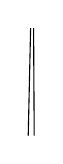
\begin{tikzpicture}[x=1ex,y=1ex]\draw (0,0)--(.2,9);\draw (.5,0)--(.45,9);\end{tikzpicture}}} there at any rate quite an interesting class of functors between modelizers
(an elementary and the basic one, for the time being\hand{)}, for which the
mere fact that the functor be compatible with weak equivalences, or only
even take aspheric objects into aspheric ones, implies that the functor
is modelizing, namely that the functor $H_M\hand{\to} H_{A^{\hand{\wedge}}}$ it induces (and the
very \uline{existen\var{\over{c}{c}}{\hand{c}}{writing over}{ps_134-4_006-v0009}e} of this functor was all we demanded \var{\inserted{beforehand!}}{\hand{beforehand!}}{insertion}{ps_134-4_006-v0010}) is actually an \uline{equi-}%
\uline{valence of categories}.

T\var{\over{h}{h}}{\hand{h}}{writing over}{ps_134-4_006-v0011}e question that immediately \hand{\unsure{.}}comes to mind now, is if this ``extra
feature'' is indeed an extremely special one, strongly dependant on the
assumptions M = (Cat) and the categories i(a) having final objects -
or if it may not have a considerably wider significance. This suggests
the still more general questions, involving two modelizers M,M' , nei-%
ther of which needs be elementary \hand{or} \var{\inserted{be}}{\hand{be}}{insertion}{ps_134-4_006-v0012}\hand{ (Cat) itself:}

\margin{6}

%% END SOURCE ps_134-4_006
\ifnum\EditionMode=1
\psapparatusstart
\psentry{ps_134-4_006-v0001}{1}{deletion}{\deleted{\xout{$\unsure{H_A = W_A^{-1}A^{\hand{\wedge}}}$}}}{}{The author cancels this material by hand; it leaves the corrected running text.}
\psentry{ps_134-4_006-v0002}{2}{authorial word join}{implic\hand{\ensuremath{\smile}}ation}{implication}{The shallow pen curve joins the c and a of implication.}
\psentry{ps_134-4_006-v0003}{3}{typewriter deletion}{\xout{condition a(iv)}}{}{The typewriter strikes out this material; it leaves the corrected running text.}
\psentry{ps_134-4_006-v0004}{4}{typed insertion}{\inserted[typed]{(a iv)\hand{$\Rightarrow$}(a ii)}}{(a iv)\hand{$\Rightarrow$}(a ii)}{The typed insertion is incorporated at its indicated position; insertion brackets leave the running text.}
\psentry{ps_134-4_006-v0005}{5}{deletion}{\deleted{Ax}}{}{The author cancels this material by hand; it leaves the corrected running text.}
\psentry{ps_134-4_006-v0006}{6}{typewriter overwriting}{\over[typed]{H}{h}}{h}{The superposed typed reading replaces the underlying reading.}
\psentry{ps_134-4_006-v0007}{7}{typewriter deletion}{\xout{\unsure{,}}}{}{The typewriter strikes out this material; it leaves the corrected running text.}
\psentry{ps_134-4_006-v0008}{8}{insertion}{\inserted{merely}}{\hand{merely}}{The handwritten insertion is incorporated at its indicated position; insertion brackets leave the running text.}
\psentry{ps_134-4_006-v0009}{9}{writing over}{\over{c}{c}}{\hand{c}}{The superposed handwritten reading replaces the underlying reading.}
\psentry{ps_134-4_006-v0010}{10}{insertion}{\inserted{beforehand!}}{\hand{beforehand!}}{The handwritten insertion is incorporated at its indicated position; insertion brackets leave the running text.}
\psentry{ps_134-4_006-v0011}{11}{writing over}{\over{h}{h}}{\hand{h}}{The superposed handwritten reading replaces the underlying reading.}
\psentry{ps_134-4_006-v0012}{12}{insertion}{\inserted{be}}{\hand{be}}{The handwritten insertion is incorporated at its indicated position; insertion brackets leave the running text.}
\psapparatusend
\fi
\pssource{ps_134-4_007}{134-4/7}{https://grothendieck.umontpellier.fr/web/viewer.html?file=../134-4.pdf\#page=8}
\psnumber{ps_134-4_007-v0001}{1}
\psnumber{ps_134-4_007-v0002}{2}
\psnumber{ps_134-4_007-v0003}{3}
\psnumber{ps_134-4_007-v0004}{4}
\psnumber{ps_134-4_007-v0005}{5}
\psnumber{ps_134-4_007-v0006}{6}
\psnumber{ps_134-4_007-v0007}{7}
\psnumber{ps_134-4_007-v0008}{8}
\psnumber{ps_134-4_007-v0009}{9}
\psnumber{ps_134-4_007-v0010}{10}
\psnumber{ps_134-4_007-v0011}{11}
\psnumber{ps_134-4_007-v0012}{12}
%% BEGIN SOURCE ps_134-4_007
% Pursuing Stacks (cotes 134-2 to 134-8): archive cote 134-4, site page 7 (PDF page 8), typescript page 95.
% typescript. Draft compared: ps3.tex:316-382.
% AI-transcribed by Claude Opus 5.5 (claude-opus-5-5, adaptive thinking, effort high), Message Batches API, batch ps1 (msgbatch_01Rv5hCaNTtUt4JHx1yqoHPL), 2026-11-12; image review recorded in records/CHECK_DECISIONS_134_3_4.tsv.
\scanpage{134-4/7}
\mspage{(95)}

\uline{Question}  Let
\[ f:\ M^{\unsure{*}}\hand{\longrightarrow} M' \]
\margin{\diagram{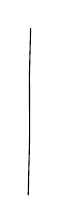
\begin{tikzpicture}[x=1ex,y=1ex]\draw (0,0)--(.12,5)--(.1,10)--(.2,14);\end{tikzpicture}}}be a functor between modelizers (M,W) and (M',W'),  assume \var{\xout{possibly}}{}{typewriter deletion}{ps_134-4_007-v0001} if
needed that f commute with  inverse limits,  or even has a left adjoint,
and that \var{\xout{projective}}{}{typewriter deletion}{ps_134-4_007-v0002} inverse limits (and direct ones too,  as f\var{\over[typed]{a}{o}}{o}{typewriter overwriting}{ps_134-4_007-v0003}r that !)
exist in M,M'.  Are there some natural conditions we\var{\xout{x}}{}{typewriter deletion}{ps_134-4_007-v0004} can devise for
M and M'  (which should be satisfied for elementary modelizers and for
the basic modelizer (Cat)),  plus possibly some \var{\over[typed]{m}{m}}{m}{typewriter overwriting}{ps_134-4_007-v0005}\var{\over[typed]{i}{i}}{i}{typewriter overwriting}{ps_134-4_007-v0006}ld extra conditions on
f itself,  which will ensure that whenever f transforms weak equivalences
into weak equivalences,  or even only aspheric objects into aspheric ob-%
jects,  f is model-preserving i.e.  $W_M = f^{-1}(W_{M'}\ )$  \uline{and} the induced funct\unsure{or}
$H_f : H_M \hand{\longrightarrow} H_{M'}$  on the localizations is an equivalence of categories.

May\var{\over[typed]{v}{b}}{b}{typewriter overwriting}{ps_134-4_007-v0007}e it's a silly question,  with pretty obvious negative answer
-  in any case,  I'll have to find out !  T\var{\over{h}{h}}{\hand{h}}{writing over}{ps_134-4_007-v0008}e very first thing to check
is to see what happens in case of a functor
\[ i^{*}\ :\ M\hand{\longrightarrow} A^{\hand{\wedge}}\ , \]
where $A^{\hand{\wedge}}$ is a weak elementary modelizer,  and where M is either (Cat) or
another weak elementary modelizer $B^{\hand{\wedge}}$,  $i^{*}$ in any case being associated of
course to a functor
\[ i:\ A\hand{\longrightarrow} M\ \ , \]
with \var{\inserted{a priori}}{\hand{a priori}}{insertion}{ps_134-4_007-v0009} no special requirement whatever on i.   In case  M = (Cat),  this
means lo\var{\over[typed]{v}{o}}{o}{typewriter overwriting}{ps_134-4_007-v0010}king up in the end the question we have postponed for \var{\inserted{quite}}{\hand{quite}}{insertion}{ps_134-4_007-v0011} a while
now,  namely of how to rescue the ``key result'' of p.61,  when dropping the
assumption that the categories i(a)  (for a in A) have final objects. We
finally got a strong motivation for carrying through a generalization,  if
this is indeed feasible.

30.3.

47.     It had become clear that the most urgent thing to do now was to
come to a better understanding of test functors with values in (Cat),  when
dropping the assumption that the categories i(a) have final objects,  and
trying to replace this (if it should turn out that something \uline{is} needed in-%
deed)  by a kind of assumption which should make sense when (Cat) is re-%
placed by a more or less arbitrary modelizer M.  I spent a few hours pon-%
dering over the situation,  and it seems to me that\hand{\unsure{,}} in the case at least
when A is a \uline{strict} test category\hand{,} namely when $A^{\hand{\wedge}}$\hand{/} is totally aspheric,  the\unsure{-}%
re is now \unsure{a} \var{\inserted[typed]{rather}}{rather}{typed insertion}{ps_134-4_007-v0012} complete understanding of the situation,  with a generalizati\unsure{-}%
on of the ``key result'' of p.61 which seems to be wholly satisfactory.

\margin{7}

%% END SOURCE ps_134-4_007
\ifnum\EditionMode=1
\psapparatusstart
\psentry{ps_134-4_007-v0001}{1}{typewriter deletion}{\xout{possibly}}{}{The typewriter strikes out this material; it leaves the corrected running text.}
\psentry{ps_134-4_007-v0002}{2}{typewriter deletion}{\xout{projective}}{}{The typewriter strikes out this material; it leaves the corrected running text.}
\psentry{ps_134-4_007-v0003}{3}{typewriter overwriting}{\over[typed]{a}{o}}{o}{The superposed typed reading replaces the underlying reading.}
\psentry{ps_134-4_007-v0004}{4}{typewriter deletion}{\xout{x}}{}{The typewriter strikes out this material; it leaves the corrected running text.}
\psentry{ps_134-4_007-v0005}{5}{typewriter overwriting}{\over[typed]{m}{m}}{m}{The superposed typed reading replaces the underlying reading.}
\psentry{ps_134-4_007-v0006}{6}{typewriter overwriting}{\over[typed]{i}{i}}{i}{The superposed typed reading replaces the underlying reading.}
\psentry{ps_134-4_007-v0007}{7}{typewriter overwriting}{\over[typed]{v}{b}}{b}{The superposed typed reading replaces the underlying reading.}
\psentry{ps_134-4_007-v0008}{8}{writing over}{\over{h}{h}}{\hand{h}}{The superposed handwritten reading replaces the underlying reading.}
\psentry{ps_134-4_007-v0009}{9}{insertion}{\inserted{a priori}}{\hand{a priori}}{The handwritten insertion is incorporated at its indicated position; insertion brackets leave the running text.}
\psentry{ps_134-4_007-v0010}{10}{typewriter overwriting}{\over[typed]{v}{o}}{o}{The superposed typed reading replaces the underlying reading.}
\psentry{ps_134-4_007-v0011}{11}{insertion}{\inserted{quite}}{\hand{quite}}{The handwritten insertion is incorporated at its indicated position; insertion brackets leave the running text.}
\psentry{ps_134-4_007-v0012}{12}{typed insertion}{\inserted[typed]{rather}}{rather}{The typed insertion is incorporated at its indicated position; insertion brackets leave the running text.}
\psapparatusend
\fi
\pssource{ps_134-4_008}{134-4/8}{https://grothendieck.umontpellier.fr/web/viewer.html?file=../134-4.pdf\#page=9}
\psnumber{ps_134-4_008-v0001}{1}
\psnumber{ps_134-4_008-v0002}{2}
\psnumber{ps_134-4_008-v0003}{3}
\psnumber{ps_134-4_008-v0004}{4}
\psnumber{ps_134-4_008-v0005}{5}
\psnumber{ps_134-4_008-v0006}{6}
\psnumber{ps_134-4_008-v0007}{7}
\psnumber{ps_134-4_008-v0008}{8}
\psnumber{ps_134-4_008-v0009}{9}
\psnumber{ps_134-4_008-v0010}{10}
\psnumber{ps_134-4_008-v0011}{11}
\psnumber{ps_134-4_008-v0012}{12}
\psnumber{ps_134-4_008-v0013}{13}
\psnumber{ps_134-4_008-v0014}{14}
\psnumber{ps_134-4_008-v0015}{15}
\psnumber{ps_134-4_008-v0016}{16}
\psnumber{ps_134-4_008-v0017}{17}
%% BEGIN SOURCE ps_134-4_008
% Pursuing Stacks (cotes 134-2 to 134-8): archive cote 134-4, site page 8 (PDF page 9), typescript page 96.
% typescript. Draft compared: ps3.tex:368-433.
% AI-transcribed by Claude Opus 5.5 (claude-opus-5-5, adaptive thinking, effort high), Message Batches API, batch ps1 (msgbatch_01Rv5hCaNTtUt4JHx1yqoHPL), 2026-11-12; image review recorded in records/CHECK_DECISIONS_134_3_4.tsv.
\scanpage{134-4/8}
\mspage{(96)}

The basic idea of how to handle the more general situation,  namely
how to compare the categories $A_{\hand{/}i^{\hand{*}}(C)} = A_{\hand{/}C}$ and $C$\hand{,} and show (under suitab%
le assumptions)  \var{that their is a canonical}{that there is a canonical}{slip corrected}{ps_134-4_008-v0001} isomorphism between their ima\var{\xout{g}}{}{typewriter deletion}{ps_134-4_008-v0002}-%
ges in the localized category $W_{Cat}^{-1}(Cat) = (Hot)$,  was around since about
the moment I worked out the ``key \var{\over[typed]{t}{r}}{r}{typewriter overwriting}{ps_134-4_008-v0003}esult''.  It can be expressed by a dia-%
gram of ``maps'' in (Cat)

% Hand-drawn arrows are marked blue; typed objects remain plain.
(1) \diagram{\begin{tikzcd} A_{\hand{/}C} \ar[r,color=blue] \& A_{\hand{//}C} \& \\ \& A\mathrm{x}C \ar[u,color=blue] \ar[r,color=blue] \& C\ , \end{tikzcd}}

where $A_{\hand{//}C}$ is the fibered category over $A$,  associated to the functor
\[ A^{opp} \hand{\longrightarrow} (Cat) \quad , \quad a \hand{\longmapsto} \underline{Hom}(i(a),C) \quad \hand{.} \]
\var{\over[typed]{H}{H}}{H}{typewriter overwriting}{ps_134-4_008-v0004}ere one should be careful \var{\over{\unsure{w}}{w}}{\hand{w}}{writing over}{ps_134-4_008-v0005}\var{\over{i}{i}}{\hand{i}}{writing over}{ps_134-4_008-v0006}th the distinction  between the \uline{set}
\[ Hom(i(a),C) = Ob\ \underline{Hom}(i(a),C)\hand{,} \]
and the \uline{category} $\underline{Hom}(i(a),C)$,  both depending bi-functorially on $a$ in $A$
and $C$ in (Cat).  The former (as a presheaf on $A$ for fixed $C$)  give\var{\over{s}{s}}{\hand{s}}{writing over}{ps_134-4_008-v0007} \var{\over{r}{r}}{\hand{r}}{writing over}{ps_134-4_008-v0008}\var{\over{i}{i}}{\hand{i}}{writing over}{ps_134-4_008-v0009}se
to $A_{\hand{/}C}$ ,  a fibered category over $A$ with \uline{discrete} fibers,  whereas the
latter gives rise to $A_{\hand{//}C}$ ,  which is fibered over $A$ with fibers which
need not be discrete.  \var{Identifiying a set}{Identifying a set}{slip corrected}{ps_134-4_008-v0010} with the discrete category it
defines,  we get a canonical functor
\[ Hom(i(a),C) \hand{\longrightarrow} \underline{Hom}(i(a),C) \ , \]
which is very far from being an equivalence nor even a weak equivalence;
being functorial f\var{\over[typed]{o}{o}}{o}{typewriter overwriting}{ps_134-4_008-v0011}r varying $a$,  it gives rise to the first map in (1).
T\var{\over[typed]{H}{h}}{h}{typewriter overwriting}{ps_134-4_008-v0012}e second is deduced from the canonical functor
\[ C \hand{\rightarrow} \underline{Hom}(i(a),C) \quad , \]
identifying $C$ with the full subcategory of \uline{constant} functors from $i(a)$ to
$C$ .  This map is functorial in $a$,  and gives rise \var{\inserted[typed]{again}}{again}{typed insertion}{ps_134-4_008-v0013} to a cartesian functor
between the corresponding fibered categories over $A$,  the first one
(which corresponds to the constant functor $A^{opp}\hand{\rightarrow}(Cat)$ with value $C$) is
just $A\mathrm{x}C$ fibered over $A$ by $pr_{1}$ ,  hence the second\var{\xout{\unsure{a}}}{}{typewriter deletion}{ps_134-4_008-v0014} arrow in (1).  The
third arrow is just $pr_{2}$ .

It seems that,  with the introduction of $A_{\hand{//}C}$,  this is the first
time since the beginning of these reflections that  we are making use of
the \uline{bicategory structure} of (Cat),  namely of the notion of a morphism,
or map or ``homotopy'' (the tie with actual homotopies will be made clear
below),  between two ``maps'' namely (here) functors  $C' \hand{\rightrightarrows} C$ .  T\var{\over[typed]{H}{h}}{h}{typewriter overwriting}{ps_134-4_008-v0015}ere is
of course a feeling that such a notion of homotopy should make a sense in
\var{\xout{rather a}}{}{typewriter deletion}{ps_134-4_008-v0016}\hand{\unsure{a}} \var{\inserted{a}}{\hand{a}}{insertion}{ps_134-4_008-v0017} more or less arbitrary modelizer $M$,  and that the approach dis-%
played by the diagram (1) may well generalize to more general situations

\margin{8}

%% END SOURCE ps_134-4_008
\ifnum\EditionMode=1
\psapparatusstart
\psentry{ps_134-4_008-v0001}{1}{slip corrected}{that their is a canonical}{that there is a canonical}{The existential construction and same-page there is settle the isolated wrong form.}
\psentry{ps_134-4_008-v0002}{2}{typewriter deletion}{\xout{g}}{}{The typewriter strikes out this material; it leaves the corrected running text.}
\psentry{ps_134-4_008-v0003}{3}{typewriter overwriting}{\over[typed]{t}{r}}{r}{The superposed typed reading replaces the underlying reading.}
\psentry{ps_134-4_008-v0004}{4}{typewriter overwriting}{\over[typed]{H}{H}}{H}{The superposed typed reading replaces the underlying reading.}
\psentry{ps_134-4_008-v0005}{5}{writing over}{\over{\unsure{w}}{w}}{\hand{w}}{The superposed handwritten reading replaces the underlying reading.}
\psentry{ps_134-4_008-v0006}{6}{writing over}{\over{i}{i}}{\hand{i}}{The superposed handwritten reading replaces the underlying reading.}
\psentry{ps_134-4_008-v0007}{7}{writing over}{\over{s}{s}}{\hand{s}}{The superposed handwritten reading replaces the underlying reading.}
\psentry{ps_134-4_008-v0008}{8}{writing over}{\over{r}{r}}{\hand{r}}{The superposed handwritten reading replaces the underlying reading.}
\psentry{ps_134-4_008-v0009}{9}{writing over}{\over{i}{i}}{\hand{i}}{The superposed handwritten reading replaces the underlying reading.}
\psentry{ps_134-4_008-v0010}{10}{slip corrected}{Identifiying a set}{Identifying a set}{The same word identifying is correctly typed later on this page.}
\psentry{ps_134-4_008-v0011}{11}{typewriter overwriting}{\over[typed]{o}{o}}{o}{The superposed typed reading replaces the underlying reading.}
\psentry{ps_134-4_008-v0012}{12}{typewriter overwriting}{\over[typed]{H}{h}}{h}{The superposed typed reading replaces the underlying reading.}
\psentry{ps_134-4_008-v0013}{13}{typed insertion}{\inserted[typed]{again}}{again}{The typed insertion is incorporated at its indicated position; insertion brackets leave the running text.}
\psentry{ps_134-4_008-v0014}{14}{typewriter deletion}{\xout{\unsure{a}}}{}{The typewriter strikes out this material; it leaves the corrected running text.}
\psentry{ps_134-4_008-v0015}{15}{typewriter overwriting}{\over[typed]{H}{h}}{h}{The superposed typed reading replaces the underlying reading.}
\psentry{ps_134-4_008-v0016}{16}{typewriter deletion}{\xout{rather a}}{}{The typewriter strikes out this material; it leaves the corrected running text.}
\psentry{ps_134-4_008-v0017}{17}{insertion}{\inserted{a}}{\hand{a}}{The handwritten insertion is incorporated at its indicated position; insertion brackets leave the running text.}
\psapparatusend
\fi
\pssource{ps_134-4_009}{134-4/9}{https://grothendieck.umontpellier.fr/web/viewer.html?file=../134-4.pdf\#page=10}
\psnumber{ps_134-4_009-v0001}{1}
\psnumber{ps_134-4_009-v0002}{2}
\psnumber{ps_134-4_009-v0003}{3}
\psnumber{ps_134-4_009-v0004}{4}
\psnumber{ps_134-4_009-v0005}{5}
\psnumber{ps_134-4_009-v0006}{6}
\psnumber{ps_134-4_009-v0007}{7}
\psnumber{ps_134-4_009-v0008}{8}
\psnumber{ps_134-4_009-v0009}{9}
\psnumber{ps_134-4_009-v0010}{10}
\psnumber{ps_134-4_009-v0011}{11}
\psnumber{ps_134-4_009-v0012}{12}
%% BEGIN SOURCE ps_134-4_009
% Pursuing Stacks (cotes 134-2 to 134-8): archive cote 134-4, site page 9 (PDF page 10), typescript page 97.
% typescript. Draft compared: ps3.tex:419-491.
% AI-transcribed by Claude Opus 5.5 (claude-opus-5-5, adaptive thinking, effort high), Message Batches API, batch ps1 (msgbatch_01Rv5hCaNTtUt4JHx1yqoHPL), 2026-11-12; image review recorded in records/CHECK_DECISIONS_134_3_4.tsv.
\scanpage{134-4/9}
\mspage{(97)}

still, with (Cat) replaced by such an M.

In the situation here, the work will consist in devising handy condi-%
tions \var{\inserted[typed]{on i: $A\hand{\rightarrow}$ (Cat)}}{on i: $A\hand{\rightarrow}$ (Cat)}{typed insertion}{ps_134-4_009-v0001} \var{\inserted{and A,}}{\hand{and A,}}{insertion}{ps_134-4_009-v0002} which will ensure that all three maps in (1) are weak equivalences,
for any choice of C. This will imply that the corresponding maps in (Hot)
are isomorphisms, hence a canonical isomorphism between the images in
(Hot) of $A_{\hand{/}C}$ and C , which will imply that a) the functor $i_A i^*$ from
(Cat) to (Cat) carries weak equivalences into weak equivalences, and
hence induces a functor
\[ (Hot) \hand{\longrightarrow} (Hot) , \]
and b) that this functor is \var{\deleted{equivalent}}{}{deletion}{ps_134-4_009-v0003} \var{\inserted{isomorphic}}{\hand{isomorphic}}{insertion}{ps_134-4_009-v0004} to the identity functor. If
moreover A is a weak test category, and therefore t$\underset{\hand{\unsure{\scriptscriptstyle z}}}{\mathrm h}$e functor
\[ W_A^{-1}A^{\hand{\wedge}} \hand{\longrightarrow} (Hot) \]
induced by $i_A$ is an equivalence, it will follow that \var{\xout{\illegible{1}\unsure{induced a}}}{}{typewriter deletion}{ps_134-4_009-v0005} \var{\inserted[typed]{\unsure{\over[typed]{i}{t}}he}}{\unsure{t}he}{typed insertion}{ps_134-4_009-v0006} functor
\[ (Hot) \hand{\longrightarrow} W_A^{-1}A^{\hand{\wedge}} \]
induced by $i^*$ is equally an equivalence, namely that $i^*$ is indeed a
test-functor.

For the map
\[ (2) \qquad AxC \hand{\rightarrow} C \]
to be a weak equivalence for any C in (Cat), it is necessary and suffi-%
cient that A be aspheric (cf. par.40, page 69), a familiar condition on
A indeed ! For handling the map
\[ (3) \qquad AxC \hand{\rightarrow} A_{\hand{//}C} \qquad \text{associated to} \quad C \hand{\rightarrow} \underline{Hom}(i(a),C) \ , \]
we'll use the following easy result (which I'll admit for the time being):
\uline{Proposition} Let F and G be two \var{\deleted{fib}}{}{deletion}{ps_134-4_009-v0007} categories over a category A, and
u: $F \hand{\rightarrow} G$ a functor compatible with projections. We assume
a) For any a in A, the induced map on the fibers
\[ u_a : F_a \hand{\rightarrow} G_a \]
is a weak equivalence.
b) Either F and G are both cofibering over A and u is cocartesian,
or F and G are fibering and i is cartesian.
T$\underset{\hand{\unsure{\scriptscriptstyle\times}}}{\mathrm h}$en u is a weak equivalence.

This shows that a sufficient condition for (3) to be a weak equivalen-%
ce, is that the functor\var{\xout{s}}{}{typewriter deletion}{ps_134-4_009-v0008} $C \hand{\rightarrow} \underline{Hom}(i(a),C)$ be a weak equivalence, for
any a in A and C in (Cat). We'll see in the next section\hand{*} that this amount\unsure{s}
to demanding that the \var{\xout{categories}}{}{typewriter deletion}{ps_134-4_009-v0009} object\var{\over[typed]{s}{s}}{s}{typewriter overwriting}{ps_134-4_009-v0010} i(a) in (Cat) should be ``contrac%
% NOTE: the right edge of the scan cuts this line after "contrac"; a hyphen may be lost
tible'', in the most concrete sense of this \var{\xout{exp}}{}{typewriter deletion}{ps_134-4_009-v0011} expression, which is ac-%
tually stronger than just asphericity. \hand{(}Earlier in these notes I was a \margin{*9.4. Actually, this is done only a lot later, on page 121 and (for the converse) on page 143.}
little floppy with the termin\var{\inserted{o}}{\hand{o}}{insertion}{ps_134-4_009-v0012}logy, by using a few times the word ``con-%

\margin{9}

%% END SOURCE ps_134-4_009
\ifnum\EditionMode=1
\psapparatusstart
\psentry{ps_134-4_009-v0001}{1}{typed insertion}{\inserted[typed]{on i: $A\hand{\rightarrow}$ (Cat)}}{on i: $A\hand{\rightarrow}$ (Cat)}{The typed insertion is incorporated at its indicated position; insertion brackets leave the running text.}
\psentry{ps_134-4_009-v0002}{2}{insertion}{\inserted{and A,}}{\hand{and A,}}{The handwritten insertion is incorporated at its indicated position; insertion brackets leave the running text.}
\psentry{ps_134-4_009-v0003}{3}{deletion}{\deleted{equivalent}}{}{The author cancels this material by hand; it leaves the corrected running text.}
\psentry{ps_134-4_009-v0004}{4}{insertion}{\inserted{isomorphic}}{\hand{isomorphic}}{The handwritten insertion is incorporated at its indicated position; insertion brackets leave the running text.}
\psentry{ps_134-4_009-v0005}{5}{typewriter deletion}{\xout{\illegible{1}\unsure{induced a}}}{}{The typewriter strikes out this material; it leaves the corrected running text.}
\psentry{ps_134-4_009-v0006}{6}{typed insertion}{\inserted[typed]{\unsure{\over[typed]{i}{t}}he}}{\unsure{t}he}{The typed insertion is incorporated at its indicated position; insertion brackets leave the running text.}
\psentry{ps_134-4_009-v0007}{7}{deletion}{\deleted{fib}}{}{The author cancels this material by hand; it leaves the corrected running text.}
\psentry{ps_134-4_009-v0008}{8}{typewriter deletion}{\xout{s}}{}{The typewriter strikes out this material; it leaves the corrected running text.}
\psentry{ps_134-4_009-v0009}{9}{typewriter deletion}{\xout{categories}}{}{The typewriter strikes out this material; it leaves the corrected running text.}
\psentry{ps_134-4_009-v0010}{10}{typewriter overwriting}{\over[typed]{s}{s}}{s}{The superposed typed reading replaces the underlying reading.}
\psentry{ps_134-4_009-v0011}{11}{typewriter deletion}{\xout{exp}}{}{The typewriter strikes out this material; it leaves the corrected running text.}
\psentry{ps_134-4_009-v0012}{12}{insertion}{\inserted{o}}{\hand{o}}{The handwritten insertion is incorporated at its indicated position; insertion brackets leave the running text.}
\psapparatusend
\fi
\pssource{ps_134-4_010}{134-4/10}{https://grothendieck.umontpellier.fr/web/viewer.html?file=../134-4.pdf\#page=11}
\psnumber{ps_134-4_010-v0001}{1}
\psnumber{ps_134-4_010-v0002}{2}
\psnumber{ps_134-4_010-v0003}{3}
\psnumber{ps_134-4_010-v0004}{4}
\psnumber{ps_134-4_010-v0005}{5}
\psnumber{ps_134-4_010-v0006}{6}
\psnumber{ps_134-4_010-v0007}{7}
\psnumber{ps_134-4_010-v0008}{8}
\psnumber{ps_134-4_010-v0009}{9}
\psnumber{ps_134-4_010-v0010}{10}
\psnumber{ps_134-4_010-v0011}{11}
\psnumber{ps_134-4_010-v0012}{12}
\psnumber{ps_134-4_010-v0013}{13}
\psnumber{ps_134-4_010-v0014}{14}
\psnumber{ps_134-4_010-v0015}{15}
\psnumber{ps_134-4_010-v0016}{16}
\psnumber{ps_134-4_010-v0017}{17}
\psnumber{ps_134-4_010-v0018}{18}
%% BEGIN SOURCE ps_134-4_010
% Pursuing Stacks (cotes 134-2 to 134-8): archive cote 134-4, site page 10 (PDF page 11), typescript page 98.
% typescript. Draft compared: ps3.tex:479-551.
% AI-transcribed by Claude Opus 5.5 (claude-opus-5-5, adaptive thinking, effort high), Message Batches API, batch ps1 (msgbatch_01Rv5hCaNTtUt4JHx1yqoHPL), 2026-11-12; image review recorded in records/CHECK_DECISIONS_134_3_4.tsv.
\scanpage{134-4/10}
\mspage{(98)}
tractible'' as synonymous to ``aspheric'', as \var{\xout{for the}}{}{typewriter deletion}{ps_134-4_010-v0001} in the context of
topological spaces, or CW spaces at any rate, the two notions do indeed
coincide, finally I came to use \var{\inserted{rather}}{\hand{rather}}{insertion}{ps_134-4_010-v0002} the word ``aspheric'' systematically, as it
fits nicely with the notion of an aspheric morphism of topoi...). T\var{\over[typed]{H}{h}}{h}{typewriter overwriting}{ps_134-4_010-v0003}e
most evident example \var{\deleted{of all}}{}{deletion}{ps_134-4_010-v0004} of contractib\var{\over[typed]{e}{l}}{l}{typewriter overwriting}{ps_134-4_010-v0005}\var{\over[typed]{l}{e}}{e}{typewriter overwriting}{ps_134-4_010-v0006} categories \var{\inserted[typed]{are}}{are}{typed insertion}{ps_134-4_010-v0007} \var{\xout{\unsure{is}}}{}{typewriter deletion}{ps_134-4_010-v0008} the categories
with final object. Thus I have the strong feeling that the condition of
contractibility of the \var{\xout{catego}}{}{typewriter deletion}{ps_134-4_010-v0009} objects $i(a)$ in (Cat) is ``the right'' genera-%
lization of the \var{\xout{condition}}{}{typewriter deletion}{ps_134-4_010-v0010} assumption made in the ``key result'', namely
that the $i(a)$\hand{'}s have final element\hand{s}. Also, it seems now likely that the
numerous cases of statements, when to check some property for arbitrary
$C$, it turned out to be enough to check it for \var{\xout{contractible}}{}{typewriter deletion}{ps_134-4_010-v0011} $C$ with a final
object, may well generalize to more general cases, with (Cat) replaced
by some $M$ and the reduction is \var{\over[typed]{f}{f}}{f}{typewriter overwriting}{ps_134-4_010-v0012}\var{\over[typed]{\unsure{o}}{r}}{r}{typewriter overwriting}{ps_134-4_010-v0013}om arbitrary $C$ in $M$ to contractible ones.

The next thing to do is to develop a little the notion of contractibi%
lity of objects and of homotopies between maps, and to get the criterion
just announced for (3) to be a weak equivalence for any $C$. After this,
handling the question of the first map in (1)
\[ \text{(4)} \qquad A_{\hand{/}C} \hand{\to} A_{\hand{//}C} \]
being a weak equivalence for any $C$, in terms of the asphericity criteri-%
on for a functor, will turn out pretty much formal, and we'll finally
be able to state a new version of the ``key result'' about test functors
$i$: $A \hand{\to}$ (\unsure{\var{\over[typed]{V}{C}}{C}{typewriter overwriting}{ps_134-4_010-v0014}}at), with \var{\inserted{this time}}{\hand{this time}}{insertion}{ps_134-4_010-v0015} twice as many equivalent formulations of the same
property. On n'arrête pas le progrès !

\hand{\unsure{Mer.}}
31.3.

48. It's time now to develop some generalities about homotopy classes
of maps, the relation of homotopy between objects of a modelizer, and the%
corresponding notion of contractibility. For the time being, it will be
enough to start with any category $M$, endowed with a set $W \hand{\subset} \mathrm{Fl}(M)$ of
arrows (the``weak equivalences''), satisfying the mild saturation assumpti-%
ons a)b)c) of par.37 (p.59). On $M$ we'll assume for the time being that
there exists (at least one) homotopy interval \var{\inserted{$\underline{I}=$}}{\hand{$\underline{I}=$}}{insertion}{ps_134-4_010-v0016}$(I,\hand{\delta}_0,\hand{\delta}_1)$ in $M$ (loc. cit.)
which implies also that $M$ has a final object, which I denote by $e_M$ or
simply \var{\over{e}{e}}{\hand{e}}{writing over}{ps_134-4_010-v0017} , and equally an initial element $\hand{\varnothing}_M$ . I'm not too sure yet whe-%
ther we'll really need that the latter be a strict initial element, as
required in the definition of a homotopy interval on page 59 (it was used
in the generalities of pages 59 and 60 only for the corollary on the Law-%
vere element ...). Whether or not will appear soon enough ! I'll not as-%
sume it till I am \var{forced too.}{forced to.}{slip corrected}{ps_134-4_010-v0018} \hand{To be safe, we'll assume on the other
hand that $M$ admits binary products.}
\margin{1°}

%% END SOURCE ps_134-4_010
\ifnum\EditionMode=1
\psapparatusstart
\psentry{ps_134-4_010-v0001}{1}{typewriter deletion}{\xout{for the}}{}{The typewriter strikes out this material; it leaves the corrected running text.}
\psentry{ps_134-4_010-v0002}{2}{insertion}{\inserted{rather}}{\hand{rather}}{The handwritten insertion is incorporated at its indicated position; insertion brackets leave the running text.}
\psentry{ps_134-4_010-v0003}{3}{typewriter overwriting}{\over[typed]{H}{h}}{h}{The superposed typed reading replaces the underlying reading.}
\psentry{ps_134-4_010-v0004}{4}{deletion}{\deleted{of all}}{}{The author cancels this material by hand; it leaves the corrected running text.}
\psentry{ps_134-4_010-v0005}{5}{typewriter overwriting}{\over[typed]{e}{l}}{l}{The superposed typed reading replaces the underlying reading.}
\psentry{ps_134-4_010-v0006}{6}{typewriter overwriting}{\over[typed]{l}{e}}{e}{The superposed typed reading replaces the underlying reading.}
\psentry{ps_134-4_010-v0007}{7}{typed insertion}{\inserted[typed]{are}}{are}{The typed insertion is incorporated at its indicated position; insertion brackets leave the running text.}
\psentry{ps_134-4_010-v0008}{8}{typewriter deletion}{\xout{\unsure{is}}}{}{The typewriter strikes out this material; it leaves the corrected running text.}
\psentry{ps_134-4_010-v0009}{9}{typewriter deletion}{\xout{catego}}{}{The typewriter strikes out this material; it leaves the corrected running text.}
\psentry{ps_134-4_010-v0010}{10}{typewriter deletion}{\xout{condition}}{}{The typewriter strikes out this material; it leaves the corrected running text.}
\psentry{ps_134-4_010-v0011}{11}{typewriter deletion}{\xout{contractible}}{}{The typewriter strikes out this material; it leaves the corrected running text.}
\psentry{ps_134-4_010-v0012}{12}{typewriter overwriting}{\over[typed]{f}{f}}{f}{The superposed typed reading replaces the underlying reading.}
\psentry{ps_134-4_010-v0013}{13}{typewriter overwriting}{\over[typed]{\unsure{o}}{r}}{r}{The superposed typed reading replaces the underlying reading.}
\psentry{ps_134-4_010-v0014}{14}{typewriter overwriting}{\over[typed]{V}{C}}{C}{The superposed typed reading replaces the underlying reading.}
\psentry{ps_134-4_010-v0015}{15}{insertion}{\inserted{this time}}{\hand{this time}}{The handwritten insertion is incorporated at its indicated position; insertion brackets leave the running text.}
\psentry{ps_134-4_010-v0016}{16}{insertion}{\inserted{$\underline{I}=$}}{\hand{$\underline{I}=$}}{The handwritten insertion is incorporated at its indicated position; insertion brackets leave the running text.}
\psentry{ps_134-4_010-v0017}{17}{writing over}{\over{e}{e}}{\hand{e}}{The superposed handwritten reading replaces the underlying reading.}
\psentry{ps_134-4_010-v0018}{18}{slip corrected}{forced too.}{forced to.}{The isolated extra o in the infinitive is settled by context and repeated to on this leaf.}
\psapparatusend
\fi
\pssource{ps_134-4_011}{134-4/11}{https://grothendieck.umontpellier.fr/web/viewer.html?file=../134-4.pdf\#page=12}
\psnumber{ps_134-4_011-v0001}{1}
\psnumber{ps_134-4_011-v0002}{2}
\psnumber{ps_134-4_011-v0003}{3}
\psnumber{ps_134-4_011-v0004}{4}
\psnumber{ps_134-4_011-v0005}{5}
\psnumber{ps_134-4_011-v0006}{6}
\psnumber{ps_134-4_011-v0007}{7}
\psnumber{ps_134-4_011-v0008}{8}
\psnumber{ps_134-4_011-v0009}{9}
\psnumber{ps_134-4_011-v0010}{10}
\psnumber{ps_134-4_011-v0011}{11}
\psnumber{ps_134-4_011-v0012}{12}
\psnumber{ps_134-4_011-v0013}{13}
\psnumber{ps_134-4_011-v0014}{14}
\psnumber{ps_134-4_011-v0015}{15}
\psnumber{ps_134-4_011-v0016}{16}
\psnumber{ps_134-4_011-v0017}{17}
\psnumber{ps_134-4_011-v0018}{18}
\psnumber{ps_134-4_011-v0019}{19}
\psnumber{ps_134-4_011-v0020}{20}
\psnumber{ps_134-4_011-v0021}{21}
%% BEGIN SOURCE ps_134-4_011
% Pursuing Stacks (cotes 134-2 to 134-8): archive cote 134-4, site page 11 (PDF page 12), typescript page 99.
% typescript. Draft compared: ps3.tex:537-605.
% AI-transcribed by Claude Opus 5.5 (claude-opus-5-5, adaptive thinking, effort high), Message Batches API, batch ps1 (msgbatch_01Rv5hCaNTtUt4JHx1yqoHPL), 2026-11-12; image review recorded in records/CHECK_DECISIONS_134_3_4.tsv.
\scanpage{134-4/11}
\mspage{\hand{99}}
Let X,Y be objects of M,  and \var{\xout{f,g}}{}{typewriter deletion}{ps_134-4_011-v0001}
\[ f,g:\ X\hand{\rightrightarrows} Y \]
two maps in M from X to Y. O\var{\over[typed]{\unsure{N}}{n}}{n}{typewriter overwriting}{ps_134-4_011-v0002}e key notion constantly used lately (but so
far only when f is an identity map,  and g a"constant"one  -  which is
equally the case needed for \var{\inserted[typed]{defining}}{defining}{typed insertion}{ps_134-4_011-v0003} \var{\xout{dealing with}}{}{typewriter deletion}{ps_134-4_011-v0004} contractibility) is the notion
of an $\underline{I}$-\uline{homotopy} \var{\xout{between}}{}{typewriter deletion}{ps_134-4_011-v0005} \uline{from} f \uline{to} g,  namely a map $F\mathrm{x}I\overset{h}{\hand{\longrightarrow}}G$  making com-%
mutative the diagram
% Hand-drawn arrows are marked blue; typed objects remain plain.
\diagram{\begin{tikzcd}
 \& F\mathrm{x}I \ar[color=blue,dd,"\hand{h}"] \& \\
F \ar[color=blue,ur,"\hand{\mathrm{id}_F\var{\over{\unsure{\times}}{\times}}{\hand{\times}}{writing over}{ps_134-4_011-v0006}\delta_0}"] \ar[color=blue,dr,swap,"\hand{f}"] \& \& \var{\over{F}{F}}{\hand{F}}{writing over}{ps_134-4_011-v0007} \ar[color=blue,ul,swap,"\hand{\mathrm{id}_F\times\delta_1}"] \ar[color=blue,dl,"\hand{g}"] \\
 \& G \&
\end{tikzcd}} .

Let's first restate the "homotopy lemma" of page 60 in a slightly more
complete form:

\uline{Homotopy lemma reformulated}:  Assume f and g are $\underline{I}$-homotopic.  Then:
a) $\hand{\gamma}(f)=\hand{\gamma}(g)$,  where
\[ \hand{\gamma}:\ M\hand{\longrightarrow} W^{-1}M = H_{M} \]
is the canonical functor.

b) If  f  is a weak equivalence,  so is g  (and conversely of course,
by symmetry\var{\deleted{\unsure{i}}}{}{deletion}{ps_134-4_011-v0008}\var{\xout{\illegible{1}}}{}{typewriter deletion}{ps_134-4_011-v0009} of the roles of $\hand{\delta}_0$ and $\hand{\delta}_1$).

c) Assume f is \var{\xout{\unsure{W}-aspheric, then so is g - and conversely}}{}{typewriter deletion}{ps_134-4_011-v0010} \var{\inserted[typed]{an isomorphism,  and g constant  -  then  F $\hand{\longrightarrow}$ e  and}}{an isomorphism,  and g constant  -  then  F $\hand{\longrightarrow}$ e  and}{typed insertion}{ps_134-4_011-v0011}
$\overset{\hand{\unsure{\hat{\ast}}}}{G}\hand{\rightarrow} e^{\hand{\unsure{\ast}}}$  are W-aspheric.

It is important to notice that the \var{\xout{notion}}{}{typewriter deletion}{ps_134-4_011-v0012} relation `` f is $\underline{I}$-homotopic
to g'' in Hom(X,Y) is not necessarily symmetric nor transitive,  and that
it depends on the choice of the homotopy interval ($\underline{I}$,$\hand{\delta}_0$,$\hand{\delta}_1$).  Thus the
symmetric relation from  $\underline{I}$-homotopy is $\hand{\check{\phantom{I}}}\!\!\underline{I}$-homotopy,  where  $\hand{\check{\phantom{I}}}\!\!\underline{I}$ is the
homotopy interval "opposite" to $\underline{I}$  (namely w\var{\over[typed]{i}{i}}{i}{typewriter overwriting}{ps_134-4_011-v0013}\var{\over[typed]{t}{t}}{t}{typewriter overwriting}{ps_134-4_011-v0014}h $\hand{\delta}_0$,$\hand{\delta}_1$ reversed).  The
example we are immediately interested in is  M = (Cat),  with $W=W_{(Cat)}$ the
usual notion of weak equivalence.  A homotopy interval is just an aspheric
small category I,  endowed with two \uline{distinct} objects  $e_0$ , $e_1$.(The condi-%
tion $e_0\hand{\neq}e_1$  just expresses the condition \var{\inserted[typed]{b)}}{b)}{typed insertion}{ps_134-4_011-v0015} $e_0\hand{\cap} e_1 = \hand{\varnothing}$  on homotopy intervals
-  if it were not satisfied,  $\underline{I}$-homotopy would just mean \var{\inserted[typed]{equality}}{equality}{typed insertion}{ps_134-4_011-v0016} \var{\xout{identity}}{}{typewriter deletion}{ps_134-4_011-v0017} of f and
g ...).  For the usual choice  $I =\hand{\Delta}_1$ =  ($e_0\hand{\rightarrow} e_1$),  an\var{\deleted{y}}{}{deletion}{ps_134-4_011-v0018} $\underline{I}$-homotopy from
f to g is just a  morphism  between functors $f\hand{\rightarrow} g$  -  the I-homotopy rela-%
tion between f and g is the existence of such a morphism,  it \var{is a\hand{\ensuremath{\backslash}}transiti%
ve}{is a transiti%
ve}{authorial word separation}{ps_134-4_011-v0019}\hand{,} and \var{\inserted[typed]{generally}}{generally}{typed insertion}{ps_134-4_011-v0020} non-symmetric relation.  If we take I to be a category with \var{\over{g}{j}}{\hand{j}}{writing over}{ps_134-4_011-v0021}ust
two objects $e_0$ and $e_1$  ,  equivalent to the final category ,  an I-homoto-%
py between f and g is  just an isomorphism from f to g  -  the I-homotopy
relation now is both transitive and symmetric,  and it is a lot more res-%
trictive than the previous one.  If we take I to be the barycentric subdi-%

\margin{11}

%% END SOURCE ps_134-4_011
\ifnum\EditionMode=1
\psapparatusstart
\psentry{ps_134-4_011-v0001}{1}{typewriter deletion}{\xout{f,g}}{}{The typewriter strikes out this material; it leaves the corrected running text.}
\psentry{ps_134-4_011-v0002}{2}{typewriter overwriting}{\over[typed]{\unsure{N}}{n}}{n}{The superposed typed reading replaces the underlying reading.}
\psentry{ps_134-4_011-v0003}{3}{typed insertion}{\inserted[typed]{defining}}{defining}{The typed insertion is incorporated at its indicated position; insertion brackets leave the running text.}
\psentry{ps_134-4_011-v0004}{4}{typewriter deletion}{\xout{dealing with}}{}{The typewriter strikes out this material; it leaves the corrected running text.}
\psentry{ps_134-4_011-v0005}{5}{typewriter deletion}{\xout{between}}{}{The typewriter strikes out this material; it leaves the corrected running text.}
\psentry{ps_134-4_011-v0006}{6}{writing over}{$\over{\unsure{\times}}{\times}$}{$\hand{\times}$}{The superposed handwritten reading replaces the underlying reading.}
\psentry{ps_134-4_011-v0007}{7}{writing over}{$\over{F}{F}$}{$\hand{F}$}{The superposed handwritten reading replaces the underlying reading.}
\psentry{ps_134-4_011-v0008}{8}{deletion}{\deleted{\unsure{i}}}{}{The author cancels this material by hand; it leaves the corrected running text.}
\psentry{ps_134-4_011-v0009}{9}{typewriter deletion}{\xout{\illegible{1}}}{}{The typewriter strikes out this material; it leaves the corrected running text.}
\psentry{ps_134-4_011-v0010}{10}{typewriter deletion}{\xout{\unsure{W}-aspheric, then so is g - and conversely}}{}{The typewriter strikes out this material; it leaves the corrected running text.}
\psentry{ps_134-4_011-v0011}{11}{typed insertion}{\inserted[typed]{an isomorphism,  and g constant  -  then  F $\hand{\longrightarrow}$ e  and}}{an isomorphism,  and g constant  -  then  F $\hand{\longrightarrow}$ e  and}{The typed insertion is incorporated at its indicated position; insertion brackets leave the running text.}
\psentry{ps_134-4_011-v0012}{12}{typewriter deletion}{\xout{notion}}{}{The typewriter strikes out this material; it leaves the corrected running text.}
\psentry{ps_134-4_011-v0013}{13}{typewriter overwriting}{\over[typed]{i}{i}}{i}{The superposed typed reading replaces the underlying reading.}
\psentry{ps_134-4_011-v0014}{14}{typewriter overwriting}{\over[typed]{t}{t}}{t}{The superposed typed reading replaces the underlying reading.}
\psentry{ps_134-4_011-v0015}{15}{typed insertion}{\inserted[typed]{b)}}{b)}{The typed insertion is incorporated at its indicated position; insertion brackets leave the running text.}
\psentry{ps_134-4_011-v0016}{16}{typed insertion}{\inserted[typed]{equality}}{equality}{The typed insertion is incorporated at its indicated position; insertion brackets leave the running text.}
\psentry{ps_134-4_011-v0017}{17}{typewriter deletion}{\xout{identity}}{}{The typewriter strikes out this material; it leaves the corrected running text.}
\psentry{ps_134-4_011-v0018}{18}{deletion}{\deleted{y}}{}{The author cancels this material by hand; it leaves the corrected running text.}
\psentry{ps_134-4_011-v0019}{19}{authorial word separation}{is a\hand{\ensuremath{\backslash}}transiti%
ve}{is a transiti%
ve}{The pen stroke separates a from transitive.}
\psentry{ps_134-4_011-v0020}{20}{typed insertion}{\inserted[typed]{generally}}{generally}{The typed insertion is incorporated at its indicated position; insertion brackets leave the running text.}
\psentry{ps_134-4_011-v0021}{21}{writing over}{\over{g}{j}}{\hand{j}}{The superposed handwritten reading replaces the underlying reading.}
\psapparatusend
\fi
\pssource{ps_134-4_012}{134-4/12}{https://grothendieck.umontpellier.fr/web/viewer.html?file=../134-4.pdf\#page=13}
\psnumber{ps_134-4_012-v0001}{1}
\psnumber{ps_134-4_012-v0002}{2}
\psnumber{ps_134-4_012-v0003}{3}
\psnumber{ps_134-4_012-v0004}{4}
\psnumber{ps_134-4_012-v0005}{5}
\psnumber{ps_134-4_012-v0006}{6}
\psnumber{ps_134-4_012-v0007}{7}
\psnumber{ps_134-4_012-v0008}{8}
\psnumber{ps_134-4_012-v0009}{9}
\psnumber{ps_134-4_012-v0010}{10}
\psnumber{ps_134-4_012-v0011}{11}
%% BEGIN SOURCE ps_134-4_012
% Pursuing Stacks (cotes 134-2 to 134-8): archive cote 134-4, site page 12 (PDF page 13), typescript page 100.
% typescript. Draft compared: ps3.tex:592-650.
% AI-transcribed by Claude Opus 5.5 (claude-opus-5-5, adaptive thinking, effort high), Message Batches API, batch ps1 (msgbatch_01Rv5hCaNTtUt4JHx1yqoHPL), 2026-11-12; image review recorded in records/CHECK_DECISIONS_134_3_4.tsv.
\scanpage{134-4/12}
\mspage{(100)}
vision of \hand{$\Delta$}$_1$,\var{\xout{with it\illegible{1}}}{}{typewriter deletion}{ps_134-4_012-v0001} which can also be interpreted as an\var{\xout{x}}{}{typewriter deletion}{ps_134-4_012-v0002} amalgamated
sum of \hand{$\Delta$}$_1$ with itself, namely
% Hand-drawn arrows are marked blue; typed objects remain plain.
$I = $ \diagram{\begin{tikzcd}[row sep=small, column sep=small] e_0 \arrow[dr,color=blue] \& \\ \& e_2 \\ e_1 \arrow[ur,color=blue] \& \end{tikzcd}} $\qquad ,$
an $\underline{I}$-homotopy from f to g is essentially a triple (k,u,v), with
k: $X \hand{\ensuremath{\to}} Y$ and u: $f \hand{\ensuremath{\to}} k$ and v: $g \hand{\ensuremath{\to}} k$ maps in \uline{Hom}(X,Y); this time, the
relation of I-homotopy is symmetric, but by no means transitive.

Returning to general M, it is customary to introduce the equivalen-%
ce relation in Hom(X,Y) generated by the relation of $\underline{I}$-homotopy - we'll
say that f and g are \uline{$\underline{I}$-homotopic in the wide sense}, and we'll write
\[ f \underset{\underline{I}}{\hand{\ensuremath{\sim}}} g \qquad , \]
if they are equivalent with respect to this relation. As seen from the \var{\xout{fi\illegible{1}}}{}{typewriter deletion}{ps_134-4_012-v0003}
\var{\deleted{first two}}{}{deletion}{ps_134-4_012-v0004} examples above (where M = (Cat))\hand{,} this relation still depends on
the choice of the homotopy interval $\underline{I}$ . Let's first look at what we can
do for fixed I, and then how what we do depends on I.

If f and g are I-homotopic, then so are their compositions with
any $Y \hand{\ensuremath{\to}} Z$ or $T \hand{\ensuremath{\to}} X$. This implies that the relation $\underset{\underline{I}}{\hand{\ensuremath{\sim}}}$ of $\underline{I}$-homotopy
in the wide sense is compatible with compositions. If we denote by
\[ \mathrm{Hom}_{\var{\deleted{\illegible{1}}}{}{deletion}{ps_134-4_012-v0005}}(X,Y)_{\underline{I}} \]
the quotient set of Hom(X,Y) by the equivalence relation of $\underline{I}$-homotopy in
the wide sense, we get composition between the sets $\mathrm{Hom}_{\var{\deleted{\illegible{1}}}{}{deletion}{ps_134-4_012-v0006}}(\var{\over[typed]{X}{X}}{X}{typewriter overwriting}{ps_134-4_012-v0007},Y)_{\underline{I}}$ , and
hence a structure of a category $M_{\underline{I}}$ having same objects as M, and where
maps from X to Y are $\underline{I}$-homotopy classes (in the wide sense - this will
be understood henceforth when speaking of homotopy classes) of maps from
X to Y in M. Two objects X,Y of M i.e. of $M_I$ which are isomorphic as
objects of $M_I$ will be called \uline{$\underline{I}$-homotopic}. This means also that we can
find maps in M \var{\inserted{(so-called \uline{$\underline{I}$-homotopisms} - namely $M_{\underline{I}}$-isomorphims)}}{\hand{(so-called \uline{$\underline{I}$-homotopisms} - namely $M_{\underline{I}}$-isomorphims)}}{insertion}{ps_134-4_012-v0008}
\[ f\colon X \hand{\ensuremath{\to}} Y \quad , \quad g\colon Y \hand{\ensuremath{\to}} X \]
such that \var{\xout{the compo}}{}{typewriter deletion}{ps_134-4_012-v0009} we get $\underline{I}$-homotopy relations in the wide sense
\[ gf \underset{\underline{I}}{\hand{\ensuremath{\sim}}} \mathrm{id}_X \quad , \quad fg \underset{\underline{I}}{\hand{\ensuremath{\sim}}} \mathrm{id}_Y \ . \]
We'll say X is \uline{$\underline{I}$-contractible} if X is $\underline{I}$-homotopic to the final object $e_M$=
e of M (which visibly is also a final object of $M_{\underline{I}}$), i.e.\var{\deleted{\xout{\unsure{this}\illegible{1}}}}{}{deletion}{ps_134-4_012-v0010} if X is a
final object of $M_{\underline{I}}$ . In terms of M, this means that there exists a
section f of X over e, such that $fp_X$ is $\underline{I}$-homotopic in the wide sense
to $\mathrm{id}_X$ (where $p_X$ is the unique map $X \hand{\ensuremath{\to}} e$). In fact, if there is such a
section f, any other section will do too.

From the homotopy lemma a) it follows that the canonical functor
\var{\deleted{\xout{$M\ \illegible{1}\ H\illegible{1}$}}}{}{deletion}{ps_134-4_012-v0011}
\margin{12}

%% END SOURCE ps_134-4_012
\ifnum\EditionMode=1
\psapparatusstart
\psentry{ps_134-4_012-v0001}{1}{typewriter deletion}{\xout{with it\illegible{1}}}{}{The typewriter strikes out this material; it leaves the corrected running text.}
\psentry{ps_134-4_012-v0002}{2}{typewriter deletion}{\xout{x}}{}{The typewriter strikes out this material; it leaves the corrected running text.}
\psentry{ps_134-4_012-v0003}{3}{typewriter deletion}{\xout{fi\illegible{1}}}{}{The typewriter strikes out this material; it leaves the corrected running text.}
\psentry{ps_134-4_012-v0004}{4}{deletion}{\deleted{first two}}{}{The author cancels this material by hand; it leaves the corrected running text.}
\psentry{ps_134-4_012-v0005}{5}{deletion}{$\deleted{\illegible{1}}$}{}{The author cancels this material by hand; it leaves the corrected running text.}
\psentry{ps_134-4_012-v0006}{6}{deletion}{$\deleted{\illegible{1}}$}{}{The author cancels this material by hand; it leaves the corrected running text.}
\psentry{ps_134-4_012-v0007}{7}{typewriter overwriting}{$\over[typed]{X}{X}$}{$X$}{The superposed typed reading replaces the underlying reading.}
\psentry{ps_134-4_012-v0008}{8}{insertion}{\inserted{(so-called \uline{$\underline{I}$-homotopisms} - namely $M_{\underline{I}}$-isomorphims)}}{\hand{(so-called \uline{$\underline{I}$-homotopisms} - namely $M_{\underline{I}}$-isomorphims)}}{The handwritten insertion is incorporated at its indicated position; insertion brackets leave the running text.}
\psentry{ps_134-4_012-v0009}{9}{typewriter deletion}{\xout{the compo}}{}{The typewriter strikes out this material; it leaves the corrected running text.}
\psentry{ps_134-4_012-v0010}{10}{deletion}{\deleted{\xout{\unsure{this}\illegible{1}}}}{}{The author cancels this material by hand; it leaves the corrected running text.}
\psentry{ps_134-4_012-v0011}{11}{deletion}{\deleted{\xout{$M\ \illegible{1}\ H\illegible{1}$}}}{}{The author cancels this material by hand; it leaves the corrected running text.}
\psapparatusend
\fi
\pssource{ps_134-4_013}{134-4/13}{https://grothendieck.umontpellier.fr/web/viewer.html?file=../134-4.pdf\#page=14}
\psnumber{ps_134-4_013-v0001}{1}
\psnumber{ps_134-4_013-v0002}{2}
\psnumber{ps_134-4_013-v0003}{3}
\psnumber{ps_134-4_013-v0004}{4}
\psnumber{ps_134-4_013-v0005}{5}
\psnumber{ps_134-4_013-v0006}{6}
\psnumber{ps_134-4_013-v0007}{7}
\psnumber{ps_134-4_013-v0008}{8}
\psnumber{ps_134-4_013-v0009}{9}
\psnumber{ps_134-4_013-v0010}{10}
\psnumber{ps_134-4_013-v0011}{11}
\psnumber{ps_134-4_013-v0012}{12}
\psnumber{ps_134-4_013-v0013}{13}
\psnumber{ps_134-4_013-v0014}{14}
\psnumber{ps_134-4_013-v0015}{15}
\psnumber{ps_134-4_013-v0016}{16}
%% BEGIN SOURCE ps_134-4_013
% Pursuing Stacks (cotes 134-2 to 134-8): archive cote 134-4, site page 13 (PDF page 14), typescript page 101.
% typescript. Draft compared: ps3.tex:635-704.
% AI-transcribed by Claude Opus 5.5 (claude-opus-5-5, adaptive thinking, effort high), Message Batches API, batch ps1 (msgbatch_01Rv5hCaNTtUt4JHx1yqoHPL), 2026-11-12; image review recorded in records/CHECK_DECISIONS_134_3_4.tsv.
\scanpage{134-4/13}
\mspage{101}

$M\hand{\longrightarrow} W^{-1}M=H_M$ factors into
\[ M\hand{\longrightarrow} M_{\underline{I}}\hand{\longrightarrow} H_M = W^{-1}M \quad , \]
and from b) it follows that if $f,g : X\hand{\rightrightarrows} Y$ are in the same \underline{I}-class, then
f is in W iff g is, hence by passage to quotient a subset
\[ W_{\underline{I}}\hand{\subset} \mathrm F\var{\over{\mathrm l}{l}}{\hand{l}}{writing over}{ps_134-4_013-v0001}(M_{\underline{I}}) \]
\var{\over[typed]{i}{o}}{o}{typewriter overwriting}{ps_134-4_013-v0002}\var{\over[typed]{n}{f}}{f}{typewriter overwriting}{ps_134-4_013-v0003} the set of arrows in $M_{\underline{I}}$ , namely a notion of \var{\xout{qua}}{}{typewriter deletion}{ps_134-4_013-v0004} weak equivalence in
$M_{\underline{I}}$ . It is evident from the universal property of $H_M$ that the canonical
functor $M_{\underline{I}}\hand{\to} H_M$ induces an isomorphism of categories
\[ H_{M_{\underline{I}}} \overset{\mathrm{def}}{=} W_{\underline{I}}^{-1}M_{\underline{I}} \hand{\xrightarrow{\ \sim\ }} H_M = W^{-1}M \quad . \]

\margin{\diagram{\begin{tikzpicture}[x=1ex,y=1ex]\draw (0,0) .. controls (.5,-.1) and (.55,.4) .. (.65,1.3)--(.8,2.3) .. controls (1.3,2.2) and (1.8,2.2) .. (2.1,2.35);\end{tikzpicture}}}It's hard at this point not to expect that $W_{\underline{I}}$ should satisfy the same mild
saturation conditions as W, so let's look into this in the \var{\over[typed]{S}{s}}{s}{typewriter overwriting}{ps_134-4_013-v0005}tri\var{\over[typed]{\unsure{l}}{d}}{d}{typewriter overwriting}{ps_134-4_013-v0006}\var{\over{e}{e}}{\hand{e}}{writing over}{ps_134-4_013-v0007} (even
though I have not had any use of this so far). Condition b) of saturation\hand{,}
namely that if f,g are composable and two among f,g,gf are in W so is the
third, carries over trivially. Condition a), namely the tautological
looking condition that W should contain all isomorphisms, makes already
a problem however. It is OK though if W satisfies the following \var{\inserted[typed]{saturation}}{saturation}{typed insertion}{ps_134-4_013-v0008} condition\hand{,}
which is a strengthening of condition c) of page 59 :

c') Let $f\colon X\hand{\longrightarrow} Y$ and $g\colon Y\hand{\longrightarrow} X$ such that $gf\hand{\in} W$ and $fg\hand{\in} W$, then
$f,g\hand{\in} W$ .

This condition c') carries over to $M_{\underline{I}}$ trivially. This suggests to intro-%
duce a strengthening of the ``mild saturation conditions'', which \var{\xout{we}}{}{typewriter deletion}{ps_134-4_013-v0009} I in-%
tend henceforth to call by the name of ``\uline{saturation}'', reserving the term
of ``\uline{strong saturation}'' to what I have previously referred to \unsure{accasionally|occasionally}
as ``saturation'' - namely the \var{\inserted{still more}}{\hand{still more}}{insertion}{ps_134-4_013-v0010} exacting condition that W consists of \uline{\var{\over{all}{all}}{\hand{all}}{writing over}{ps_134-4_013-v0011}}
arrows made invertible by the localization functor $M\hand{\longrightarrow} H_M=W^{-1}M$, or
equivalently, by some functor $M\hand{\to} H$ . \var{\inserted{Thus}}{\hand{Thus}}{insertion}{ps_134-4_013-v0012} We'll say W is \uline{saturated} if it
satisfies the following :

a') For any X in M, $\mathrm{id}_X\hand{\in} W$ .

b') Same as b) before: if two among f,g,gf are in W, so is the thi\hand{rd}

c') If $f\colon X\hand{\to} Y$ and $g\colon Y\hand{\to} X$ are such that $gf,\var{\over{gf}{gf}}{\hand{gf}}{writing over}{ps_134-4_013-v0013}\hand{\in} W$, then $f,g\hand{\in} W$ .

Each of these conditions carries over from W to a $W_{\underline{I}}$ trivially.

I can't help either having a look at the most evident exactness pro-%
perties of the canonical functor $M\hand{\to} M_{\underline{I}}$ \unsure{?} Thus one immediately sees
that for two maps
\[ f,g : X\hand{\rightrightarrows} Y=Y_1\mathrm{x}Y_2 \quad \unsure{\mathrm n}, \]
with components $f_i$ , $g_i$ ($i\hand{\in}\hand{\{1,2\}}$), f and g are I-homotopic \var{\inserted{in the wide sense}}{\hand{in the wide sense}}{insertion}{ps_134-4_013-v0014} iff so are
$f_i$ and $g_i$ (for $i\hand{\in}\hand{\{1,2\}}$). The analoguous statement is valid for \var{\xout{any}}{}{typewriter deletion}{ps_134-4_013-v0015} maps
into any product object $Y=\hand{\prod} Y_i$ \var{\deleted{- not necessarily}}{}{deletion}{ps_134-4_013-v0016} on a finite set of

\margin{13}

%% END SOURCE ps_134-4_013
\ifnum\EditionMode=1
\psapparatusstart
\psentry{ps_134-4_013-v0001}{1}{writing over}{$\over{\mathrm l}{l}$}{$\hand{l}$}{The superposed handwritten reading replaces the underlying reading.}
\psentry{ps_134-4_013-v0002}{2}{typewriter overwriting}{\over[typed]{i}{o}}{o}{The superposed typed reading replaces the underlying reading.}
\psentry{ps_134-4_013-v0003}{3}{typewriter overwriting}{\over[typed]{n}{f}}{f}{The superposed typed reading replaces the underlying reading.}
\psentry{ps_134-4_013-v0004}{4}{typewriter deletion}{\xout{qua}}{}{The typewriter strikes out this material; it leaves the corrected running text.}
\psentry{ps_134-4_013-v0005}{5}{typewriter overwriting}{\over[typed]{S}{s}}{s}{The superposed typed reading replaces the underlying reading.}
\psentry{ps_134-4_013-v0006}{6}{typewriter overwriting}{\over[typed]{\unsure{l}}{d}}{d}{The superposed typed reading replaces the underlying reading.}
\psentry{ps_134-4_013-v0007}{7}{writing over}{\over{e}{e}}{\hand{e}}{The superposed handwritten reading replaces the underlying reading.}
\psentry{ps_134-4_013-v0008}{8}{typed insertion}{\inserted[typed]{saturation}}{saturation}{The typed insertion is incorporated at its indicated position; insertion brackets leave the running text.}
\psentry{ps_134-4_013-v0009}{9}{typewriter deletion}{\xout{we}}{}{The typewriter strikes out this material; it leaves the corrected running text.}
\psentry{ps_134-4_013-v0010}{10}{insertion}{\inserted{still more}}{\hand{still more}}{The handwritten insertion is incorporated at its indicated position; insertion brackets leave the running text.}
\psentry{ps_134-4_013-v0011}{11}{writing over}{\over{all}{all}}{\hand{all}}{The superposed handwritten reading replaces the underlying reading.}
\psentry{ps_134-4_013-v0012}{12}{insertion}{\inserted{Thus}}{\hand{Thus}}{The handwritten insertion is incorporated at its indicated position; insertion brackets leave the running text.}
\psentry{ps_134-4_013-v0013}{13}{writing over}{$\over{gf}{gf}$}{$\hand{gf}$}{The superposed handwritten reading replaces the underlying reading.}
\psentry{ps_134-4_013-v0014}{14}{insertion}{\inserted{in the wide sense}}{\hand{in the wide sense}}{The handwritten insertion is incorporated at its indicated position; insertion brackets leave the running text.}
\psentry{ps_134-4_013-v0015}{15}{typewriter deletion}{\xout{any}}{}{The typewriter strikes out this material; it leaves the corrected running text.}
\psentry{ps_134-4_013-v0016}{16}{deletion}{\deleted{- not necessarily}}{}{The author cancels this material by hand; it leaves the corrected running text.}
\psapparatusend
\fi
\pssource{ps_134-4_014}{134-4/14}{https://grothendieck.umontpellier.fr/web/viewer.html?file=../134-4.pdf\#page=15}
\psnumber{ps_134-4_014-v0001}{1}
\psnumber{ps_134-4_014-v0002}{2}
\psnumber{ps_134-4_014-v0003}{3}
\psnumber{ps_134-4_014-v0004}{4}
\psnumber{ps_134-4_014-v0005}{5}
\psnumber{ps_134-4_014-v0006}{6}
\psnumber{ps_134-4_014-v0007}{7}
\psnumber{ps_134-4_014-v0008}{8}
\psnumber{ps_134-4_014-v0009}{9}
\psnumber{ps_134-4_014-v0010}{10}
\psnumber{ps_134-4_014-v0011}{11}
\psnumber{ps_134-4_014-v0012}{12}
\psnumber{ps_134-4_014-v0013}{13}
\psnumber{ps_134-4_014-v0014}{14}
\psnumber{ps_134-4_014-v0015}{15}
\psnumber{ps_134-4_014-v0016}{16}
\psnumber{ps_134-4_014-v0017}{17}
\psnumber{ps_134-4_014-v0018}{18}
\psnumber{ps_134-4_014-v0019}{19}
\psnumber{ps_134-4_014-v0020}{20}
\psnumber{ps_134-4_014-v0021}{21}
\psnumber{ps_134-4_014-v0022}{22}
\psnumber{ps_134-4_014-v0023}{23}
\psnumber{ps_134-4_014-v0024}{24}
\psnumber{ps_134-4_014-v0025}{25}
\psnumber{ps_134-4_014-v0026}{26}
\psnumber{ps_134-4_014-v0027}{27}
\psnumber{ps_134-4_014-v0028}{28}
%% BEGIN SOURCE ps_134-4_014
% Pursuing Stacks (cotes 134-2 to 134-8): archive cote 134-4, site page 14 (PDF page 15), typescript page 102.
% typescript. Draft compared: ps3.tex:691-761.
% AI-transcribed by Claude Opus 5.5 (claude-opus-5-5, adaptive thinking, effort high), Message Batches API, batch ps1 (msgbatch_01Rv5hCaNTtUt4JHx1yqoHPL), 2026-11-12; image review recorded in records/CHECK_DECISIONS_134_3_4.tsv.
\scanpage{134-4/14}
\mspage{102}
indices.  T\var{\over{H}{h}}{\hand{h}}{writing over}{ps_134-4_014-v0001}e dual statement so to say,  when X is decomposed as a sum
$X = \hand{\coprod} X_i$ ,  is valid too,  provided taking products with I is distributive
with respect to \var{\inserted{finite}}{\hand{finite}}{insertion}{ps_134-4_014-v0002} direct sums.  Thus we get that $M \hand{\to} M_{\underline{I}}$  commutes with \var{\deleted{ar-}}{}{deletion}{ps_134-4_014-v0003}%
\var{\deleted{bitrary}}{}{deletion}{ps_134-4_014-v0004} \var{\inserted{finite}}{\hand{finite}}{insertion}{ps_134-4_014-v0005} \var{\xout{\illegible{1}}}{}{typewriter deletion}{ps_134-4_014-v0006} products,  and with \var{\deleted{arbitrary}}{}{deletion}{ps_134-4_014-v0007} \var{\inserted{finite}}{\hand{finite}}{insertion}{ps_134-4_014-v0008} sums too provided they are dis-%
tributive with respect to multiplication with any object  (or \var{\inserted{with}}{\hand{with}}{insertion}{ps_134-4_014-v0009} I \var{\over{only}{only}}{\hand{only}}{writing over}{ps_134-4_014-v0010},
which would be enough).

The notion of $\underline{I}$-homotopy in the wide sense between $f,g\colon X \hand{\rightrightarrows} Y$ can
be interpreted in terms of strict $\underline{I}'$-homotopy with variable $\underline{I}'$ ,  as fol-%
lows,  provided we make some mild extra assumptions on (M,W), namely:

a)  (Just for memory)  M is stable under finite products.

b)  M is stable under amalgamated sums  $I \hand{\amalg}_e J$  under the final ob-%
ject e (I and J endowed with sections over e).

c)  If moreover I and J are aspheric over e ,  then so is $I \hand{\amalg}_e J$.

Conditions \var{\over{\unsure{a}}{b}}{\hand{b}}{writing over}{ps_134-4_014-v0011}) and \var{\over{\unsure{b}}{c}}{\hand{c}}{writing over}{ps_134-4_014-v0012}) give a means of constructing new homotopy inter-%
vals \var{\inserted[typed]{$\underline{K}$}}{$\underline{K}$}{typed insertion}{ps_134-4_014-v0013},  by amalgamating two \var{\inserted[typed]{homotopy}}{homotopy}{typed insertion}{ps_134-4_014-v0014} intervals  $\underline{I}$ and $\underline{J}$ ,  using as sections \var{\xout{for}}{}{typewriter deletion}{ps_134-4_014-v0015}
of $\underline{I}$ and $\underline{J}$ for making the amalgamation,  either \var{$\hand{\ensuremath{\delta}}_0$ of $\hand{\ensuremath{\delta}}_1$}{$\hand{\ensuremath{\delta}}_0$ or $\hand{\ensuremath{\delta}}_1$}{slip corrected}{ps_134-4_014-v0016} ,  which gives
four ways of amalgamating  -  of course we take as endpoints of the amal-%
gamat\var{\over{e}{e}}{\hand{e}}{writing over}{ps_134-4_014-v0017}\var{\over{d}{d}}{\hand{d}}{writing over}{ps_134-4_014-v0018}\var{\xout{\illegible{1}}}{}{typewriter deletion}{ps_134-4_014-v0019} interval, \var{\inserted[typed]{the}}{the}{typed insertion}{ps_134-4_014-v0020} sections over e coming from the two endpoints of
$\underline{I}$  (giving rise to $\hand{\ensuremath{\delta}}_0$ \var{\inserted[typed]{for $\underline{K}$}}{for $\underline{K}$}{typed insertion}{ps_134-4_014-v0021}) and $\underline{J}$  (giving rise to $\hand{\ensuremath{\delta}}_1$ for $\underline{K}$) which have not
been ``used up'' in the amalgamation.  Maybe the handiest convention is to
define \uline{the}  amalgamated interval $\underline{I}\hand{\vee}\underline{J}$ ,  without any ambiguity of choice,
as being
\[\begin{aligned}& \var{\xout{\underline{K}}}{}{typewriter deletion}{ps_134-4_014-v0022}\ \underline{I}\hand{\vee}\underline{J} = (I,\hand{\ensuremath{\delta}}_1^{\hand{\ensuremath{I}}})\hand{\amalg}_e(J,\hand{\ensuremath{\delta}}_0^{\hand{\ensuremath{J}}}) \\ &\text{endowed with  the two sections coming from } \hand{\ensuremath{\delta}}_0^{\hand{\ensuremath{I}}}\colon e\hand{\to} I \ , \ \hand{\ensuremath{\delta}}_1^{\hand{\ensuremath{J}}}\colon e\hand{\to} J \ , \end{aligned}\]
and defining the three other choices \var{\xout{by\illegible{1}}}{}{typewriter deletion}{ps_134-4_014-v0023} in terms of this operation,  by
replacing one or two among the summands $\underline{I}$, $\underline{J}$  by the ``opposite'' interval
$\overset{\hand{\ensuremath{\vee}}}{\underline{I}}$  or  $\overset{\hand{\ensuremath{\vee}}}{\underline{J}}$ .  T\var{\over[typed]{H}{h}}{h}{typewriter overwriting}{ps_134-4_014-v0024}e operation of amalgamation of intervals,  and likewise of
homotopy intervals,  just defined,  is clearly associative up to canonical
isomorphism,  and we have a canonical isomorphism of intervals
\[ (\underline{I}\hand{\vee}\underline{J})^{\hand{\ensuremath{\vee}}} \hand{\simeq} \overset{\hand{\ensuremath{\vee}}}{\underline{I}}\hand{\vee}\overset{\hand{\ensuremath{\vee}}}{\underline{J}} \ . \]
I forgot to check,  for amalgamation of homotopy intervals,  the condition
b) of page 59 namely $e_0 \hand{\cap} e_1 = \hand{\varnothing}_M$  (which has not so far played any role,
anyhow).  To get this condition,  we'll have to be slightly more specific
in condition b) above on M of existence of the relevant amalgamations,
by demanding (as suggested of course by the visual intuition of the situa-%
tion)  that I and \var{\over[typed]{\unsure{U}}{J}}{J}{typewriter overwriting}{ps_134-4_014-v0025}  should become subobjects of the amalgamation K,  and
their intersection should be reduce\var{\over{\illegible{1}}{d}}{\hand{d}}{writing over}{ps_134-4_014-v0026} to \var{\over[typed]{t}{t}}{t}{typewriter overwriting}{ps_134-4_014-v0027}he tautological part e of it.
M$\overset{\hand{\smile}}{\mathrm o}$re relevant still for the use we have in mind is to demand that those
amalgamations should commute to products b\var{\over{y}{y}}{\hand{y}}{writing over}{ps_134-4_014-v0028} an arbitrary element X of M.

\margin{14}

%% END SOURCE ps_134-4_014
\ifnum\EditionMode=1
\psapparatusstart
\psentry{ps_134-4_014-v0001}{1}{writing over}{\over{H}{h}}{\hand{h}}{The superposed handwritten reading replaces the underlying reading.}
\psentry{ps_134-4_014-v0002}{2}{insertion}{\inserted{finite}}{\hand{finite}}{The handwritten insertion is incorporated at its indicated position; insertion brackets leave the running text.}
\psentry{ps_134-4_014-v0003}{3}{deletion}{\deleted{ar-}}{}{The author cancels this material by hand; it leaves the corrected running text.}
\psentry{ps_134-4_014-v0004}{4}{deletion}{\deleted{bitrary}}{}{The author cancels this material by hand; it leaves the corrected running text.}
\psentry{ps_134-4_014-v0005}{5}{insertion}{\inserted{finite}}{\hand{finite}}{The handwritten insertion is incorporated at its indicated position; insertion brackets leave the running text.}
\psentry{ps_134-4_014-v0006}{6}{typewriter deletion}{\xout{\illegible{1}}}{}{The typewriter strikes out this material; it leaves the corrected running text.}
\psentry{ps_134-4_014-v0007}{7}{deletion}{\deleted{arbitrary}}{}{The author cancels this material by hand; it leaves the corrected running text.}
\psentry{ps_134-4_014-v0008}{8}{insertion}{\inserted{finite}}{\hand{finite}}{The handwritten insertion is incorporated at its indicated position; insertion brackets leave the running text.}
\psentry{ps_134-4_014-v0009}{9}{insertion}{\inserted{with}}{\hand{with}}{The handwritten insertion is incorporated at its indicated position; insertion brackets leave the running text.}
\psentry{ps_134-4_014-v0010}{10}{writing over}{\over{only}{only}}{\hand{only}}{The superposed handwritten reading replaces the underlying reading.}
\psentry{ps_134-4_014-v0011}{11}{writing over}{\over{\unsure{a}}{b}}{\hand{b}}{The superposed handwritten reading replaces the underlying reading.}
\psentry{ps_134-4_014-v0012}{12}{writing over}{\over{\unsure{b}}{c}}{\hand{c}}{The superposed handwritten reading replaces the underlying reading.}
\psentry{ps_134-4_014-v0013}{13}{typed insertion}{\inserted[typed]{$\underline{K}$}}{$\underline{K}$}{The typed insertion is incorporated at its indicated position; insertion brackets leave the running text.}
\psentry{ps_134-4_014-v0014}{14}{typed insertion}{\inserted[typed]{homotopy}}{homotopy}{The typed insertion is incorporated at its indicated position; insertion brackets leave the running text.}
\psentry{ps_134-4_014-v0015}{15}{typewriter deletion}{\xout{for}}{}{The typewriter strikes out this material; it leaves the corrected running text.}
\psentry{ps_134-4_014-v0016}{16}{slip corrected}{$\hand{\ensuremath{\delta}}_0$ of $\hand{\ensuremath{\delta}}_1$}{$\hand{\ensuremath{\delta}}_0$ or $\hand{\ensuremath{\delta}}_1$}{The isolated of in either/or alternatives is settled by context and same-page or.}
\psentry{ps_134-4_014-v0017}{17}{writing over}{\over{e}{e}}{\hand{e}}{The superposed handwritten reading replaces the underlying reading.}
\psentry{ps_134-4_014-v0018}{18}{writing over}{\over{d}{d}}{\hand{d}}{The superposed handwritten reading replaces the underlying reading.}
\psentry{ps_134-4_014-v0019}{19}{typewriter deletion}{\xout{\illegible{1}}}{}{The typewriter strikes out this material; it leaves the corrected running text.}
\psentry{ps_134-4_014-v0020}{20}{typed insertion}{\inserted[typed]{the}}{the}{The typed insertion is incorporated at its indicated position; insertion brackets leave the running text.}
\psentry{ps_134-4_014-v0021}{21}{typed insertion}{\inserted[typed]{for $\underline{K}$}}{for $\underline{K}$}{The typed insertion is incorporated at its indicated position; insertion brackets leave the running text.}
\psentry{ps_134-4_014-v0022}{22}{typewriter deletion}{$\xout{\underline{K}}$}{}{The typewriter strikes out this material; it leaves the corrected running text.}
\psentry{ps_134-4_014-v0023}{23}{typewriter deletion}{\xout{by\illegible{1}}}{}{The typewriter strikes out this material; it leaves the corrected running text.}
\psentry{ps_134-4_014-v0024}{24}{typewriter overwriting}{\over[typed]{H}{h}}{h}{The superposed typed reading replaces the underlying reading.}
\psentry{ps_134-4_014-v0025}{25}{typewriter overwriting}{\over[typed]{\unsure{U}}{J}}{J}{The superposed typed reading replaces the underlying reading.}
\psentry{ps_134-4_014-v0026}{26}{writing over}{\over{\illegible{1}}{d}}{\hand{d}}{The superposed handwritten reading replaces the underlying reading.}
\psentry{ps_134-4_014-v0027}{27}{typewriter overwriting}{\over[typed]{t}{t}}{t}{The superposed typed reading replaces the underlying reading.}
\psentry{ps_134-4_014-v0028}{28}{writing over}{\over{y}{y}}{\hand{y}}{The superposed handwritten reading replaces the underlying reading.}
\psapparatusend
\fi
\pssource{ps_134-4_015}{134-4/15}{https://grothendieck.umontpellier.fr/web/viewer.html?file=../134-4.pdf\#page=16}
\psnumber{ps_134-4_015-v0001}{1}
\psnumber{ps_134-4_015-v0002}{2}
\psnumber{ps_134-4_015-v0003}{3}
\psnumber{ps_134-4_015-v0004}{4}
\psnumber{ps_134-4_015-v0005}{5}
\psnumber{ps_134-4_015-v0006}{6}
\psnumber{ps_134-4_015-v0007}{7}
\psnumber{ps_134-4_015-v0008}{8}
\psnumber{ps_134-4_015-v0009}{9}
\psnumber{ps_134-4_015-v0010}{10}
\psnumber{ps_134-4_015-v0011}{11}
\psnumber{ps_134-4_015-v0012}{12}
\psnumber{ps_134-4_015-v0013}{13}
\psnumber{ps_134-4_015-v0014}{14}
%% BEGIN SOURCE ps_134-4_015
% Pursuing Stacks (cotes 134-2 to 134-8): archive cote 134-4, site page 15 (PDF page 16), typescript page 103.
% typescript. Draft compared: ps3.tex:747-809.
% AI-transcribed by Claude Opus 5.5 (claude-opus-5-5, adaptive thinking, effort high), Message Batches API, batch ps1 (msgbatch_01Rv5hCaNTtUt4JHx1yqoHPL), 2026-11-12; image review recorded in records/CHECK_DECISIONS_134_3_4.tsv.
\scanpage{134-4/15}
\mspage{103}
This I'll assume in the interpretation of $\underset{\underline{I}}{\hand{\sim}}$ in terms of strict homoto-%
pies. Namely, let
\[ \mathrm{Comp}(\underline{I}) \]
be the set of all homotopy intervals deduced from $\underline{I}$ by taking amalgama-%
tions of \var{\over{\underline{I}}{c}}{\hand{c}}{writing over}{ps_134-4_015-v0001}opies of $\underline{I}$ and $\overset{\hand{\vee}}{\underline{I}}$ , with an arbitrary number $n \hand{\geq} 1$ of summands.
Thus we get just $\underline{I}$ and $\overset{\hand{\vee}}{\underline{I}}$ for $n=1$, four intervals for \var{\over[typed]{i}{n}}{n}{typewriter overwriting}{ps_134-4_015-v0002}$=2$, ..., $2^n$ inter-%
vals for $n$ arbitrary . It is now immediately checked that for $f,g$ in
$\mathrm{Hom}(X,Y)$, \var{\deleted{\xout{f and}}}{}{deletion}{ps_134-4_015-v0003} the relation $f \underset{\underline{I}}{\hand{\sim}} g$ is equivalent to the existence of
$\underline{K} \hand{\in} \mathrm{Comp}(\underline{I})$ , such that $f$ and $g$ be $\underline{K}$-homotopic (in the strict sense).

\uline{Remark} T\var{\over[typed]{H}{h}}{h}{typewriter overwriting}{ps_134-4_015-v0004}e saturation conditions a')b')c') on \var{\xout{\unsure{we}}}{}{typewriter deletion}{ps_134-4_015-v0005} $W$ are easily checked
for the usual notion of weak equivalence for morphisms of topoi, and hence
also in the categories \var{\xout{of the type}}{}{typewriter deletion}{ps_134-4_015-v0006} (Cat) and in any topos, and therefore
in any category $A^{\hand{\overset{\wedge}{\wedge}}}$ (where it boils down \var{\inserted[typed]{too}}{too}{typed insertion}{ps_134-4_015-v0007} to the corresponding properties
on $W_{(\mathrm{Cat})}$ , as $W_A = i_A^{-1}(W_{(\mathrm{Cat})}$ ). Thus it \var{\deleted{\unsure{s}}}{}{deletion}{ps_134-4_015-v0008}seems definitely reasonabl\unsure{e}
henceforth to take these as the standart notion of saturation (referring \var{\xout{t}}{}{typewriter deletion}{ps_134-4_015-v0009}
to it's variants by the qualifications ``mild'' or ``strong''). On the other
hand, the stability conditions a)b)c) on $(M,W)$ are satisfied whenever $M$
is a topos, with the usual notion of weak equivalence - the condition
c') being a consequence of the more general \var{\inserted[typed]{Mayer-Vietoris type}}{Mayer-Vietoris type}{typed insertion}{ps_134-4_015-v0010} statement about amalgamations
of topoi under closed embeddings of such (cf. lemma on page \hspace{2em}). T$\underset{\hand{\unsure{\wedge}}}{\mathrm h}$e
same should hold in (Cat), with a similar Mayer-Vietoris argument -
there is a slight trouble here for applying the precedent result on
amalgamation of topoi, because a section $e \hand{\to} C$ of an \var{\deleted{\xout{category}}}{}{deletion}{ps_134-4_015-v0011} object $C$
of (Cat), namely an embedding of the one-point category $e=\hand{\Delta_0}$ into $C$ by
choice of an object of $C$, does not correspond in general to a closed
embedding of topoi. (In geometrical language, we get a ``point'' of the
topos $C^{\hand{\wedge}}$ defined by $C$, but a point need not correspond to a subtopos,
let alone a closed one ...). This shows the asphericity criterion for
amalgamation of topoi, and hence also for amal\var{\over{\unsure{j|g}}{g}}{\hand{g}}{writing over}{ps_134-4_015-v0012}\var{\over{a}{a}}{\hand{a}}{writing over}{ps_134-4_015-v0013}mation of categories,
has not been cut out with sufficient generality yet. As this whole
$\mathrm{Comp}(\underline{I})$ story is just a digression for the time being, I'll leave it at
that now.

M$\overset{\hand{\smile}}{\mathrm o}$re important than amalgamation of intervals, is to compare the
notions of homotopy defined in terms of a\var{\xout{n inter}}{}{typewriter deletion}{ps_134-4_015-v0014} homotopy interval $\underline{I}$, to
the corresponding notions for another interval\hand{,} $\underline{J}$ . Here the natural idea
first is to see what happens if we got a morphism of intervals (compatible
with endpoints, by definition)
\[ \underline{J} \hand{\to} \underline{I} \quad . \]

\margin{15}

%% END SOURCE ps_134-4_015
\ifnum\EditionMode=1
\psapparatusstart
\psentry{ps_134-4_015-v0001}{1}{writing over}{\over{\underline{I}}{c}}{\hand{c}}{The superposed handwritten reading replaces the underlying reading.}
\psentry{ps_134-4_015-v0002}{2}{typewriter overwriting}{\over[typed]{i}{n}}{n}{The superposed typed reading replaces the underlying reading.}
\psentry{ps_134-4_015-v0003}{3}{deletion}{\deleted{\xout{f and}}}{}{The author cancels this material by hand; it leaves the corrected running text.}
\psentry{ps_134-4_015-v0004}{4}{typewriter overwriting}{\over[typed]{H}{h}}{h}{The superposed typed reading replaces the underlying reading.}
\psentry{ps_134-4_015-v0005}{5}{typewriter deletion}{\xout{\unsure{we}}}{}{The typewriter strikes out this material; it leaves the corrected running text.}
\psentry{ps_134-4_015-v0006}{6}{typewriter deletion}{\xout{of the type}}{}{The typewriter strikes out this material; it leaves the corrected running text.}
\psentry{ps_134-4_015-v0007}{7}{typed insertion}{\inserted[typed]{too}}{too}{The typed insertion is incorporated at its indicated position; insertion brackets leave the running text.}
\psentry{ps_134-4_015-v0008}{8}{deletion}{\deleted{\unsure{s}}}{}{The author cancels this material by hand; it leaves the corrected running text.}
\psentry{ps_134-4_015-v0009}{9}{typewriter deletion}{\xout{t}}{}{The typewriter strikes out this material; it leaves the corrected running text.}
\psentry{ps_134-4_015-v0010}{10}{typed insertion}{\inserted[typed]{Mayer-Vietoris type}}{Mayer-Vietoris type}{The typed insertion is incorporated at its indicated position; insertion brackets leave the running text.}
\psentry{ps_134-4_015-v0011}{11}{deletion}{\deleted{\xout{category}}}{}{The author cancels this material by hand; it leaves the corrected running text.}
\psentry{ps_134-4_015-v0012}{12}{writing over}{\over{\unsure{j|g}}{g}}{\hand{g}}{The superposed handwritten reading replaces the underlying reading.}
\psentry{ps_134-4_015-v0013}{13}{writing over}{\over{a}{a}}{\hand{a}}{The superposed handwritten reading replaces the underlying reading.}
\psentry{ps_134-4_015-v0014}{14}{typewriter deletion}{\xout{n inter}}{}{The typewriter strikes out this material; it leaves the corrected running text.}
\psapparatusend
\fi
\pssource{ps_134-4_016}{134-4/16}{https://grothendieck.umontpellier.fr/web/viewer.html?file=../134-4.pdf\#page=17}
\psnumber{ps_134-4_016-v0001}{1}
\psnumber{ps_134-4_016-v0002}{2}
\psnumber{ps_134-4_016-v0003}{3}
\psnumber{ps_134-4_016-v0004}{4}
\psnumber{ps_134-4_016-v0005}{5}
\psnumber{ps_134-4_016-v0006}{6}
\psnumber{ps_134-4_016-v0007}{7}
\psnumber{ps_134-4_016-v0008}{8}
\psnumber{ps_134-4_016-v0009}{9}
\psnumber{ps_134-4_016-v0010}{10}
\psnumber{ps_134-4_016-v0011}{11}
\psnumber{ps_134-4_016-v0012}{12}
\psnumber{ps_134-4_016-v0013}{13}
\psnumber{ps_134-4_016-v0014}{14}
\psnumber{ps_134-4_016-v0015}{15}
\psnumber{ps_134-4_016-v0016}{16}
\psnumber{ps_134-4_016-v0017}{17}
\psnumber{ps_134-4_016-v0018}{18}
%% BEGIN SOURCE ps_134-4_016
% Pursuing Stacks (cotes 134-2 to 134-8): archive cote 134-4, site page 16 (PDF page 17), typescript page 104.
% typescript. Draft compared: ps3.tex:793-853.
% AI-transcribed by Claude Opus 5.5 (claude-opus-5-5, adaptive thinking, effort high), Message Batches API, batch ps1 (msgbatch_01Rv5hCaNTtUt4JHx1yqoHPL), 2026-11-12; image review recorded in records/CHECK_DECISIONS_134_3_4.tsv.
\scanpage{134-4/16}
\mspage{104}
It is clear then,  for $f,g\hand{\in}\mathrm{Hom}(X,Y)$,  that any $\underline{I}$-homotopy from f to g
gives rise to a $\underline{J}$-homotopy; hence if f and g are $\underline{I}$-homotopic they are
$\underline{J}$-homotopic,  and hence the same for homotopy in the wide sense.  We get
thus a \var{\inserted[typed]{canonical}}{canonical}{typed insertion}{ps_134-4_016-v0001} functor
\[ M_{\underline{I}} \hand{\to} M_{\underline{J}} \]
which is the identity on objects,  entering into a cascade of canonical
functors
\[ M \hand{\to} M_{\underline{I}} \hand{\longrightarrow} M_{\underline{J}} \hand{\to} H \ , \]
\var{\xout{where $H$ \unsure{is} $= H_M = W^{-1}M$}}{}{typewriter deletion}{ps_134-4_016-v0002}
where  $H=H_M= W^{-1} M$  can be viewed as the common localization of $M,M_{\underline{I}},M_{\underline{J}}$
with respect to the notion of weak equivalences in these categories.  We
may view $M_{\underline{J}}$  as a closer approximation to H than $M_{\underline{I}}$ .  T\var{\over[typed]{H}{h}}{h}{typewriter overwriting}{ps_134-4_016-v0003}ere  is of course
an evident transitivity relation for the functors corresponding to two
composable morphisms of intervals
\[ \underline{K} \hand{\to} \underline{J} \hand{\to} \underline{I} \quad . \]
\uline{R\var{\over[typed]{E}{e}}{e}{typewriter overwriting}{ps_134-4_016-v0004}mark}.  \var{\over[typed]{I}{I}}{I}{typewriter overwriting}{ps_134-4_016-v0005}n order to get that $\underset{\underline{I}}{\hand{\sim}}$ implies $\underset{\underline{J}}{\hand{\sim}}$ ,  it is sufficient to
make a much weaker assumption than existence of a morphism of intervals
$\underline{J}\hand{\to}\underline{I}$  -  namely it suffices to assume that the two sections $\hand{\delta}^{\underline{I}}_{i}$ : e $\hand{\to} \underline{I}$
are $\underline{J}$-homotopic.  M$\overset{\hand{\unsure{\smile}}}{\underset{\hand{\wedge}}{\mathrm o}}$re generally,  let $\hand{\sim}$ be an equivalence relation in
F\var{\over{l}{l}}{\hand{l}}{writing over}{ps_134-4_016-v0006}(M),  compatible with compositions and with cartesian products (this is
the case indeed for $\underset{\underline{J}}{\hand{\sim}}$ ),  and let  $\underline{I} \var{\over{\unsure{b}}{=}}{\hand{=}}{writing over}{ps_134-4_016-v0007} (I,\hand{\delta}_0,\hand{\delta}_1)$ any object I \var{\inserted[typed]{of M}}{of M}{typed insertion}{ps_134-4_016-v0008} (not neces-%
sarily aspheric over e) endowed with two sections over e ,  such that
$\hand{\delta}_0\hand{\sim}\hand{\delta}_1$ .   Then the interval $\underline{I}$ gives rise to an equivalence relation $\underset{\underline{I}}{\hand{\sim}}$
in F\var{\over{l}{l}}{\hand{l}}{writing over}{ps_134-4_016-v0009}(M) , whose definition is quite independant of W -  and a priori
\var{\xout{(if it were not for the condition}}{}{typewriter deletion}{ps_134-4_016-v0010} if  $f\underset{\underline{I}}{\hand{\sim}}g$  and $f\hand{\in}W$,  this need not
imply $g\hand{\in}W$.  However,  the condition $\hand{\delta}_0\hand{\sim}\hand{\delta}_1$  implies immediately that the
\var{\xout{condition}}{}{typewriter deletion}{ps_134-4_016-v0011} relation  $\underset{\underline{I}}{\hand{\sim}}$  implies the relation $\hand{\sim}$ .  When the latter is
$\underset{\underline{J}}{\hand{\sim}}$ ,  we get moreover that W is the inverse image of a set of arrows in
$M_{\underline{I}}$ , \hand{i.e. $f\underset{I}{\sim}g$ and $f\in W$ implies $g\in W$.}

   An interesting particular case is the one when we can find a homotopy
interval  $\underline{I}_0$  in \var{\over{M}{M}}{\hand{M}}{writing over}{ps_134-4_016-v0012} ,  which has the property that for any other homotopy
interval $\underline{I}$ in M,  it's structural sections satisfy
\[ \hand{\delta}^{\underline{I}}_0 \underset{\underline{I}_0}{\hand{\sim}} \hand{\delta}^{\underline{I}}_1 \qquad . \]
This implies that the homotopy relation $\underset{\underline{I}_0}{\hand{\sim}}$ is implied by all other simi-%
lar relations $\underset{\underline{I}}{\hand{\sim}}$ ,  i.e. it is the coarsest among all relations $\underset{\underline{I}}{\hand{\sim}}$ .  We
may \var{\xout{call}}{}{typewriter deletion}{ps_134-4_016-v0013} then view $\underline{I}_0$ as a ``\uline{fundamental}'' or ``\uline{characteristic}'' \uline{homotopy
interval} in M,  in the sense that \var{\xout{to check if}}{}{typewriter deletion}{ps_134-4_016-v0014} \var{\inserted[typed]{the relation}}{the relation}{typed insertion}{ps_134-4_016-v0015} $f\underset{W}{\hand{\sim}}g$  in the sense below ,
namely \var{\deleted{\xout{if there exis\illegible{1}}}}{}{deletion}{ps_134-4_016-v0016} \var{\inserted[typed]{existence of}}{existence of}{typed insertion}{ps_134-4_016-v0017} a homotopy  interval $\underline{I}$ such that $f\underset{\underline{I}}{\hand{\sim}}g$ ,  is equi-%
valent to  $f\underset{\underline{I}_0}{\hand{\sim}}g$  i.e. can be checked using \var{\inserted[typed]{\over[typed]{T}{t}he}}{the}{typed insertion}{ps_134-4_016-v0018} one and unique  $\underline{I}_0$ .  In the
case of M=(Cat\hand{)},  we get readily $\hand{\Delta}_1$ as a characteristic homotopy inter-
\margin{16}

%% END SOURCE ps_134-4_016
\ifnum\EditionMode=1
\psapparatusstart
\psentry{ps_134-4_016-v0001}{1}{typed insertion}{\inserted[typed]{canonical}}{canonical}{The typed insertion is incorporated at its indicated position; insertion brackets leave the running text.}
\psentry{ps_134-4_016-v0002}{2}{typewriter deletion}{\xout{where $H$ \unsure{is} $= H_M = W^{-1}M$}}{}{The typewriter strikes out this material; it leaves the corrected running text.}
\psentry{ps_134-4_016-v0003}{3}{typewriter overwriting}{\over[typed]{H}{h}}{h}{The superposed typed reading replaces the underlying reading.}
\psentry{ps_134-4_016-v0004}{4}{typewriter overwriting}{\over[typed]{E}{e}}{e}{The superposed typed reading replaces the underlying reading.}
\psentry{ps_134-4_016-v0005}{5}{typewriter overwriting}{\over[typed]{I}{I}}{I}{The superposed typed reading replaces the underlying reading.}
\psentry{ps_134-4_016-v0006}{6}{writing over}{\over{l}{l}}{\hand{l}}{The superposed handwritten reading replaces the underlying reading.}
\psentry{ps_134-4_016-v0007}{7}{writing over}{$\over{\unsure{b}}{=}$}{$\hand{=}$}{The superposed handwritten reading replaces the underlying reading.}
\psentry{ps_134-4_016-v0008}{8}{typed insertion}{\inserted[typed]{of M}}{of M}{The typed insertion is incorporated at its indicated position; insertion brackets leave the running text.}
\psentry{ps_134-4_016-v0009}{9}{writing over}{\over{l}{l}}{\hand{l}}{The superposed handwritten reading replaces the underlying reading.}
\psentry{ps_134-4_016-v0010}{10}{typewriter deletion}{\xout{(if it were not for the condition}}{}{The typewriter strikes out this material; it leaves the corrected running text.}
\psentry{ps_134-4_016-v0011}{11}{typewriter deletion}{\xout{condition}}{}{The typewriter strikes out this material; it leaves the corrected running text.}
\psentry{ps_134-4_016-v0012}{12}{writing over}{\over{M}{M}}{\hand{M}}{The superposed handwritten reading replaces the underlying reading.}
\psentry{ps_134-4_016-v0013}{13}{typewriter deletion}{\xout{call}}{}{The typewriter strikes out this material; it leaves the corrected running text.}
\psentry{ps_134-4_016-v0014}{14}{typewriter deletion}{\xout{to check if}}{}{The typewriter strikes out this material; it leaves the corrected running text.}
\psentry{ps_134-4_016-v0015}{15}{typed insertion}{\inserted[typed]{the relation}}{the relation}{The typed insertion is incorporated at its indicated position; insertion brackets leave the running text.}
\psentry{ps_134-4_016-v0016}{16}{deletion}{\deleted{\xout{if there exis\illegible{1}}}}{}{The author cancels this material by hand; it leaves the corrected running text.}
\psentry{ps_134-4_016-v0017}{17}{typed insertion}{\inserted[typed]{existence of}}{existence of}{The typed insertion is incorporated at its indicated position; insertion brackets leave the running text.}
\psentry{ps_134-4_016-v0018}{18}{typed insertion}{\inserted[typed]{\over[typed]{T}{t}he}}{the}{The typed insertion is incorporated at its indicated position; insertion brackets leave the running text.}
\psapparatusend
\fi
\pssource{ps_134-4_017}{134-4/17}{https://grothendieck.umontpellier.fr/web/viewer.html?file=../134-4.pdf\#page=18}
\psnumber{ps_134-4_017-v0001}{1}
\psnumber{ps_134-4_017-v0002}{2}
\psnumber{ps_134-4_017-v0003}{3}
\psnumber{ps_134-4_017-v0004}{4}
\psnumber{ps_134-4_017-v0005}{5}
\psnumber{ps_134-4_017-v0006}{6}
\psnumber{ps_134-4_017-v0007}{7}
\psnumber{ps_134-4_017-v0008}{8}
\psnumber{ps_134-4_017-v0009}{9}
\psnumber{ps_134-4_017-v0010}{10}
\psnumber{ps_134-4_017-v0011}{11}
\psnumber{ps_134-4_017-v0012}{12}
\psnumber{ps_134-4_017-v0013}{13}
\psnumber{ps_134-4_017-v0014}{14}
\psnumber{ps_134-4_017-v0015}{15}
\psnumber{ps_134-4_017-v0016}{16}
\psnumber{ps_134-4_017-v0017}{17}
\psnumber{ps_134-4_017-v0018}{18}
\psnumber{ps_134-4_017-v0019}{19}
\psnumber{ps_134-4_017-v0020}{20}
%% BEGIN SOURCE ps_134-4_017
% Pursuing Stacks (cotes 134-2 to 134-8): archive cote 134-4, site page 17 (PDF page 18), typescript page 105.
% typescript. Draft compared: ps3.tex:841-901.
% AI-transcribed by Claude Opus 5.5 (claude-opus-5-5, adaptive thinking, effort high), Message Batches API, batch ps1 (msgbatch_01Rv5hCaNTtUt4JHx1yqoHPL), 2026-11-12; image review recorded in records/CHECK_DECISIONS_134_3_4.tsv.
\scanpage{134-4/17}
\mspage{105}
val. More specifically, if $\hand{\delta}_o,\hand{\delta}_1 : e \hand{\longrightarrow} I$ are two se\unsure{\var{\over[typed]{v}{c}}{c}{typewriter overwriting}{ps_134-4_017-v0001}}tions of an
object I of (Cat), i.e. two objects $e_o,e_1$ of the small category I, then
these are $\hand{\Delta}_1$ -homotopic iff $e_o,e_1$ belong to the same connected component
of I, which is automatic if I is 0-connected, and a fortiori if I is
aspheric. This accounts to a great extent, it seems, for the important
role $\hand{\Delta}_1$ is playing in the homotopy theory of (Cat), and consequently in
the whole foundational set-up I am developping here, using (Cat) as the
basic ``modelizer''.

It is not clear to me for the time being whether it is reasonable to
e\var{\over{x}{x}}{\hand{x}}{writing over}{ps_134-4_017-v0002}pect in more or less any modelizer (M,W) the existence of a characteris\var{\xout{t}}{}{typewriter deletion}{ps_134-4_017-v0003}%
tic homotopy interval (provided of course a homotopy interval exists).
This is certainly the case for the elementary modelizers met so far. Pre-%
sumably I'll have to come back upon this question sooner or later.

\var{\xout{We'll now see}}{}{typewriter deletion}{ps_134-4_017-v0004}
We'll now see that the set of equivalence relations $\underset{\underline{I}}{\hand{\sim}}$ on F\var{\over{l}{l}}{\hand{l}}{writing over}{ps_134-4_017-v0005}(M) ,
indexed by the set of homotopy intervals $\underline{I}$ , is ``filtrant d\'ecr\var{\over{\unsure{a}}{o}}{\hand{o}}{writing over}{ps_134-4_017-v0006}issant'',
namely that for two such relations $\underset{\underline{I}}{\hand{\sim}}$ and $\underset{\underline{J}}{\hand{\sim}}$ ,,\var{\over[typed]{t}{t}}{t}{typewriter overwriting}{ps_134-4_017-v0007}here is a third \var{\inserted{``wider''}}{\hand{``wider''}}{insertion}{ps_134-4_017-v0008} one\hand{,}
$\underset{\underline{K}}{\hand{\sim}}$ implied by both. It is enough to construct a $\underline{K}$, endowed with morphism\unsure{s}
\[ \underline{K} \hand{\longrightarrow} \underline{I} \ , \ \underline{K} \hand{\longrightarrow} \underline{J} \]
of homotopy intervals. I\var{\over[typed]{n}{n}}{n}{typewriter overwriting}{ps_134-4_017-v0009}deed, there is a universal choice, namely the
category of homotopy intervals admits binary products - we'll take thus
\[ \underline{K} = \underline{I} \text{ x } \underline{J} \ , \]
where the underlying object of M is just IxJ, endowed with the two sec-%
tions $\hand{\delta}^{\underline{I}}_{i}$x$\hand{\delta}^{\underline{J}}_{i}$ \hand{$(i\in\{0,1\})$.}

As usual, we'll denote by $\underset{W}{\hand{\sim}}$ or simply $\hand{\sim}$ the equivalence relation
on F\var{\over{l}{l}}{\hand{l}}{writing over}{ps_134-4_017-v0010}(M), which is the limit \var{\inserted[typed]{or union}}{or union}{typed insertion}{ps_134-4_017-v0011} of the equivalence relations $\underset{\underline{I}}{\hand{\sim}}$ - in
other words
\[ f\underset{W}{\hand{\sim}}g \quad \text{iff exists } \underline{I}\text{ , a homotopy interval in M , with } f\underset{\underline{I}}{\hand{\sim}}g. \]
For X,Y in M, we'll denote by \var{\deleted{Hom(X}}{}{deletion}{ps_134-4_017-v0012}
\[ \mathrm{Hom}(X,Y)_W \]
the quotient of Hom(X,Y) by the previous equivalence relation. This rela-%
tion is clearly compatible with compositions, and hence we get a category
$M_W$ , having same objects as M , which can be equally viewed as the \var{\xout{categor}}{}{typewriter deletion}{ps_134-4_017-v0013}
filtering limit of the categories $M_{\var{\over[typed]{\illegible{1}}{\underline{I}}}{\underline{I}}{typewriter overwriting}{ps_134-4_017-v0014}}$ .
\[ M_W \ = \ \underset{\underline{I}}{\underset{\hand{\longrightarrow}}{\mathrm{lim}}} \ M_{\underline{I}} \quad , \]
where we \var{\inserted[typed]{may}}{may}{typed insertion}{ps_134-4_017-v0015} \var{\xout{\illegible{1}}}{}{typewriter deletion}{ps_134-4_017-v0016} take as indexing set for the limit the \var{\deleted{ordered}}{}{deletion}{ps_134-4_017-v0017} set of all $\underline{I}$'s\hand{,}
\var{\deleted{and \xout{the relation of domination} write}}{}{deletion}{ps_134-4_017-v0018} \var{\inserted{preordered by}}{\hand{preordered by}}{insertion}{ps_134-4_017-v0019} $\underline{I}\hand{\leqslant}\underline{J}$ i\hand{ff} there exists a morphism of
intervals $\underline{J}\hand{\to}\underline{I}$ (its the \var{\inserted{pre}}{\hand{pre}}{insertion}{ps_134-4_017-v0020}order relation opposite to the usual one on the

\margin{17}

%% END SOURCE ps_134-4_017
\ifnum\EditionMode=1
\psapparatusstart
\psentry{ps_134-4_017-v0001}{1}{typewriter overwriting}{\over[typed]{v}{c}}{c}{The superposed typed reading replaces the underlying reading.}
\psentry{ps_134-4_017-v0002}{2}{writing over}{\over{x}{x}}{\hand{x}}{The superposed handwritten reading replaces the underlying reading.}
\psentry{ps_134-4_017-v0003}{3}{typewriter deletion}{\xout{t}}{}{The typewriter strikes out this material; it leaves the corrected running text.}
\psentry{ps_134-4_017-v0004}{4}{typewriter deletion}{\xout{We'll now see}}{}{The typewriter strikes out this material; it leaves the corrected running text.}
\psentry{ps_134-4_017-v0005}{5}{writing over}{\over{l}{l}}{\hand{l}}{The superposed handwritten reading replaces the underlying reading.}
\psentry{ps_134-4_017-v0006}{6}{writing over}{\over{\unsure{a}}{o}}{\hand{o}}{The superposed handwritten reading replaces the underlying reading.}
\psentry{ps_134-4_017-v0007}{7}{typewriter overwriting}{\over[typed]{t}{t}}{t}{The superposed typed reading replaces the underlying reading.}
\psentry{ps_134-4_017-v0008}{8}{insertion}{\inserted{``wider''}}{\hand{``wider''}}{The handwritten insertion is incorporated at its indicated position; insertion brackets leave the running text.}
\psentry{ps_134-4_017-v0009}{9}{typewriter overwriting}{\over[typed]{n}{n}}{n}{The superposed typed reading replaces the underlying reading.}
\psentry{ps_134-4_017-v0010}{10}{writing over}{\over{l}{l}}{\hand{l}}{The superposed handwritten reading replaces the underlying reading.}
\psentry{ps_134-4_017-v0011}{11}{typed insertion}{\inserted[typed]{or union}}{or union}{The typed insertion is incorporated at its indicated position; insertion brackets leave the running text.}
\psentry{ps_134-4_017-v0012}{12}{deletion}{\deleted{Hom(X}}{}{The author cancels this material by hand; it leaves the corrected running text.}
\psentry{ps_134-4_017-v0013}{13}{typewriter deletion}{\xout{categor}}{}{The typewriter strikes out this material; it leaves the corrected running text.}
\psentry{ps_134-4_017-v0014}{14}{typewriter overwriting}{$\over[typed]{\illegible{1}}{\underline{I}}$}{$\underline{I}$}{The superposed typed reading replaces the underlying reading.}
\psentry{ps_134-4_017-v0015}{15}{typed insertion}{\inserted[typed]{may}}{may}{The typed insertion is incorporated at its indicated position; insertion brackets leave the running text.}
\psentry{ps_134-4_017-v0016}{16}{typewriter deletion}{\xout{\illegible{1}}}{}{The typewriter strikes out this material; it leaves the corrected running text.}
\psentry{ps_134-4_017-v0017}{17}{deletion}{\deleted{ordered}}{}{The author cancels this material by hand; it leaves the corrected running text.}
\psentry{ps_134-4_017-v0018}{18}{deletion}{\deleted{and \xout{the relation of domination} write}}{}{The author cancels this material by hand; it leaves the corrected running text.}
\psentry{ps_134-4_017-v0019}{19}{insertion}{\inserted{preordered by}}{\hand{preordered by}}{The handwritten insertion is incorporated at its indicated position; insertion brackets leave the running text.}
\psentry{ps_134-4_017-v0020}{20}{insertion}{\inserted{pre}}{\hand{pre}}{The handwritten insertion is incorporated at its indicated position; insertion brackets leave the running text.}
\psapparatusend
\fi
\pssource{ps_134-4_018}{134-4/18}{https://grothendieck.umontpellier.fr/web/viewer.html?file=../134-4.pdf\#page=19}
\psnumber{ps_134-4_018-v0001}{1}
\psnumber{ps_134-4_018-v0002}{2}
\psnumber{ps_134-4_018-v0003}{3}
\psnumber{ps_134-4_018-v0004}{4}
\psnumber{ps_134-4_018-v0005}{5}
\psnumber{ps_134-4_018-v0006}{6}
\psnumber{ps_134-4_018-v0007}{7}
\psnumber{ps_134-4_018-v0008}{8}
\psnumber{ps_134-4_018-v0009}{9}
\psnumber{ps_134-4_018-v0010}{10}
\psnumber{ps_134-4_018-v0011}{11}
\psnumber{ps_134-4_018-v0012}{12}
\psnumber{ps_134-4_018-v0013}{13}
\psnumber{ps_134-4_018-v0014}{14}
\psnumber{ps_134-4_018-v0015}{15}
\psnumber{ps_134-4_018-v0016}{16}
\psnumber{ps_134-4_018-v0017}{17}
\psnumber{ps_134-4_018-v0018}{18}
\psnumber{ps_134-4_018-v0019}{19}
\psnumber{ps_134-4_018-v0020}{20}
\psnumber{ps_134-4_018-v0021}{21}
\psnumber{ps_134-4_018-v0022}{22}
\psnumber{ps_134-4_018-v0023}{23}
\psnumber{ps_134-4_018-v0024}{24}
%% BEGIN SOURCE ps_134-4_018
% Pursuing Stacks (cotes 134-2 to 134-8): archive cote 134-4, site page 18 (PDF page 19), typescript page 106.
% typescript. Draft compared: ps3.tex:886-940.
% AI-transcribed by Claude Opus 5.5 (claude-opus-5-5, adaptive thinking, effort high), Message Batches API, batch ps1 (msgbatch_01Rv5hCaNTtUt4JHx1yqoHPL), 2026-11-12; image review recorded in records/CHECK_DECISIONS_134_3_4.tsv.
\scanpage{134-4/18}
\mspage{106}
set of objects of a category ...).

We now get canonical functors
\[ M\hand{\longrightarrow} M_{\underline{I}} \hand{\to} M_W \hand{\to} H \quad , \]
where H can again be considered as the common localization of the three
categories M, $M_{\underline{I}}$ (any $\underline{I}$), $M_W$ with respect to the notion of weak equivalen%
ce in each, It is clear that the set of weak equivalences in $M_W$ , say $\overset{\hand{\rule{0.65em}{0.4pt}}}{W}$,
is saturated provided W is. Also, the canonical functor $M\hand{\to} M_{\var{\over[typed]{\illegible{1}}{W}}{W}{typewriter overwriting}{ps_134-4_018-v0001}}$ commutes
with finite products, and also with finite sums provided formation of
such sums in M commutes with taking products \var{\over{w}{w}}{\hand{w}}{writing over}{ps_134-4_018-v0002}\var{\over{\unsure{i|j}}{i}}{\hand{i}}{writing over}{ps_134-4_018-v0003}\var{\over{t}{t}}{\hand{t}}{writing over}{ps_134-4_018-v0004}h \var{\deleted{a}}{}{deletion}{ps_134-4_018-v0005}\var{\inserted[typed]{any}}{any}{typed insertion}{ps_134-4_018-v0006} fixed element of M.
\var{\deleted{T\over{h}{h}e same statement will hold for infinite products or sums, provided we
assume there exists a characteristic homotopy interval \inserted[typed]{$\underline{I}_o$}, in M, so that we
got a description
\[ M_W \qquad M_{\underline{I}_o} \quad , \]
and may apply the \xout{result} corresponding fact for M \quad $M_{\underline{I}_o}$ .}}{}{deletion}{ps_134-4_018-v0007}

A map f: $X\hand{\to} Y$ is called a \var{\inserted{\uline{homotopy equivalence} or}}{\hand{\uline{homotopy equivalence} or}}{insertion}{ps_134-4_018-v0008} \uline{homotopism} (with respect to W) if it is
an isomorphism in $M_W$ , namely if there exists g: $Y\hand{\to} X$ such that
\[ gf \underset{W}{\hand{\sim}} \mathrm{id}_X \quad , \quad fg \underset{W}{\hand{\sim}} \mathrm{id}_Y \quad . \]
\var{\inserted[typed]{This implies f and g are weak equivalences.}}{This implies f and g are weak equivalences.}{typed insertion}{ps_134-4_018-v0009}
\var{\xout{When X\illegible{1}simpl}}{}{typewriter deletion}{ps_134-4_018-v0010}\hand{\ensuremath{\unsure{\lozenge}}} If such an f exists namely if X and Y are isomorphic
objects of $M_{\var{\over{W}{W}}{\hand{W}}{writing over}{ps_134-4_018-v0011}}$ , we'll say they are \var{\inserted[typed]{W-}}{W-}{typed insertion}{ps_134-4_018-v0012}\uline{homotopic}, or simply \uline{homotopic}. This
implies that there \var{\xout{are}}{}{typewriter deletion}{ps_134-4_018-v0013}\var{\inserted[typed]{exist}}{exist}{typed insertion}{ps_134-4_018-v0014} weak equivalences $X\hand{\to} Y$ and $Y\hand{\to} X$, but the con-%
verse of course is'nt always true. If Y is the final object $e_M$ , we'll
say X is W-\uline{contractible} (or simply \var{\uline{contactible}}{\uline{contractible}}{slip corrected}{ps_134-4_018-v0015}) \var{\xout{in order}}{}{typewriter deletion}{ps_134-4_018-v0016} instead of
W-homotopic to Y\hand{$=e$.} In case there exists a characteristic homotopy
interval $\underline{I}_o$ , all these W-notions boil down to the corresponding $\underline{I}_o$-noti-%
ons considered before.

\var{\inserted{\uline{Remark.}}}{\hand{\uline{Remark.}}}{insertion}{ps_134-4_018-v0017} It occurs to me that in all what precedes, we never made any use
really of the existence of a homotopy interval\var{\over{\unsure{.}}{!}}{\hand{!}}{writing over}{ps_134-4_018-v0018} T\var{\over[typed]{H}{h}}{h}{typewriter overwriting}{ps_134-4_018-v0019}e only notion we have
been effectively been working with, it seems to me, is the notion\unsure{s} of
``weak homotopy interval'', by which I mean a\var{\xout{n object}}{}{typewriter deletion}{ps_134-4_018-v0020} triple $(\underline{I},\hand{\ensuremath{\delta}}_o,\hand{\ensuremath{\delta}}_1)$
satisfying merely the condition \var{\xout{a) and (\illegible{1}) of page 59}}{}{typewriter deletion}{ps_134-4_018-v0021} that I be aspheric
over e (which is the condition c) on page 59). Such an \underline{I} always exists
of course, we need only take I = e itself ! I\var{\over[typed]{f}{n}}{n}{typewriter overwriting}{ps_134-4_018-v0022} \var{\inserted[typed]{case}}{case}{typed insertion}{ps_134-4_018-v0023} however an \var{\inserted{actual}}{\hand{actual}}{insertion}{ps_134-4_018-v0024} homotopy
interval (with Ker$(\hand{\ensuremath{\delta}}_o,\hand{\ensuremath{\delta}}_1) = \hand{\varnothing}_M$ ) does exist, to make sure that the notion
of W-homotopy obtained by using all weak homotopy intervals is the same
as when using only actual homotopy intervals, we should be sure that
for any I aspheric over e, any two sections $\hand{\ensuremath{\delta}}_o,\hand{\ensuremath{\delta}}_1$ of I over e are W-homo-%
topic in the initial meaning. This is evidently so when M = (Cat) and
W = $\hand{\ensuremath{\mathcal{W}}}_{(Cat)}$ (indeed, it is enough that I be O-connected, instead of

\margin{18}

%% END SOURCE ps_134-4_018
\ifnum\EditionMode=1
\psapparatusstart
\psentry{ps_134-4_018-v0001}{1}{typewriter overwriting}{$\over[typed]{\illegible{1}}{W}$}{$W$}{The superposed typed reading replaces the underlying reading.}
\psentry{ps_134-4_018-v0002}{2}{writing over}{\over{w}{w}}{\hand{w}}{The superposed handwritten reading replaces the underlying reading.}
\psentry{ps_134-4_018-v0003}{3}{writing over}{\over{\unsure{i|j}}{i}}{\hand{i}}{The superposed handwritten reading replaces the underlying reading.}
\psentry{ps_134-4_018-v0004}{4}{writing over}{\over{t}{t}}{\hand{t}}{The superposed handwritten reading replaces the underlying reading.}
\psentry{ps_134-4_018-v0005}{5}{deletion}{\deleted{a}}{}{The author cancels this material by hand; it leaves the corrected running text.}
\psentry{ps_134-4_018-v0006}{6}{typed insertion}{\inserted[typed]{any}}{any}{The typed insertion is incorporated at its indicated position; insertion brackets leave the running text.}
\psentry{ps_134-4_018-v0007}{7}{deletion}{\deleted{T\over{h}{h}e same statement will hold for infinite products or sums, provided we
assume there exists a characteristic homotopy interval \inserted[typed]{$\underline{I}_o$}, in M, so that we
got a description
\[ M_W \qquad M_{\underline{I}_o} \quad , \]
and may apply the \xout{result} corresponding fact for M \quad $M_{\underline{I}_o}$ .}}{}{The author cancels this material by hand; it leaves the corrected running text.}
\psentry{ps_134-4_018-v0008}{8}{insertion}{\inserted{\uline{homotopy equivalence} or}}{\hand{\uline{homotopy equivalence} or}}{The handwritten insertion is incorporated at its indicated position; insertion brackets leave the running text.}
\psentry{ps_134-4_018-v0009}{9}{typed insertion}{\inserted[typed]{This implies f and g are weak equivalences.}}{This implies f and g are weak equivalences.}{The typed insertion is incorporated at its indicated position; insertion brackets leave the running text.}
\psentry{ps_134-4_018-v0010}{10}{typewriter deletion}{\xout{When X\illegible{1}simpl}}{}{The typewriter strikes out this material; it leaves the corrected running text.}
\psentry{ps_134-4_018-v0011}{11}{writing over}{$\over{W}{W}$}{$\hand{W}$}{The superposed handwritten reading replaces the underlying reading.}
\psentry{ps_134-4_018-v0012}{12}{typed insertion}{\inserted[typed]{W-}}{W-}{The typed insertion is incorporated at its indicated position; insertion brackets leave the running text.}
\psentry{ps_134-4_018-v0013}{13}{typewriter deletion}{\xout{are}}{}{The typewriter strikes out this material; it leaves the corrected running text.}
\psentry{ps_134-4_018-v0014}{14}{typed insertion}{\inserted[typed]{exist}}{exist}{The typed insertion is incorporated at its indicated position; insertion brackets leave the running text.}
\psentry{ps_134-4_018-v0015}{15}{slip corrected}{\uline{contactible}}{\uline{contractible}}{One-off omitted r, with contractible correctly typed in the same sentence.}
\psentry{ps_134-4_018-v0016}{16}{typewriter deletion}{\xout{in order}}{}{The typewriter strikes out this material; it leaves the corrected running text.}
\psentry{ps_134-4_018-v0017}{17}{insertion}{\inserted{\uline{Remark.}}}{\hand{\uline{Remark.}}}{The handwritten insertion is incorporated at its indicated position; insertion brackets leave the running text.}
\psentry{ps_134-4_018-v0018}{18}{writing over}{\over{\unsure{.}}{!}}{\hand{!}}{The superposed handwritten reading replaces the underlying reading.}
\psentry{ps_134-4_018-v0019}{19}{typewriter overwriting}{\over[typed]{H}{h}}{h}{The superposed typed reading replaces the underlying reading.}
\psentry{ps_134-4_018-v0020}{20}{typewriter deletion}{\xout{n object}}{}{The typewriter strikes out this material; it leaves the corrected running text.}
\psentry{ps_134-4_018-v0021}{21}{typewriter deletion}{\xout{a) and (\illegible{1}) of page 59}}{}{The typewriter strikes out this material; it leaves the corrected running text.}
\psentry{ps_134-4_018-v0022}{22}{typewriter overwriting}{\over[typed]{f}{n}}{n}{The superposed typed reading replaces the underlying reading.}
\psentry{ps_134-4_018-v0023}{23}{typed insertion}{\inserted[typed]{case}}{case}{The typed insertion is incorporated at its indicated position; insertion brackets leave the running text.}
\psentry{ps_134-4_018-v0024}{24}{insertion}{\inserted{actual}}{\hand{actual}}{The handwritten insertion is incorporated at its indicated position; insertion brackets leave the running text.}
\psapparatusend
\fi
\pssource{ps_134-4_019}{134-4/19}{https://grothendieck.umontpellier.fr/web/viewer.html?file=../134-4.pdf\#page=20}
\psnumber{ps_134-4_019-v0001}{1}
\psnumber{ps_134-4_019-v0002}{2}
\psnumber{ps_134-4_019-v0003}{3}
\psnumber{ps_134-4_019-v0004}{4}
\psnumber{ps_134-4_019-v0005}{5}
\psnumber{ps_134-4_019-v0006}{6}
\psnumber{ps_134-4_019-v0007}{7}
\psnumber{ps_134-4_019-v0008}{8}
\psnumber{ps_134-4_019-v0009}{9}
\psnumber{ps_134-4_019-v0010}{10}
\psnumber{ps_134-4_019-v0011}{11}
\psnumber{ps_134-4_019-v0012}{12}
\psnumber{ps_134-4_019-v0013}{13}
\psnumber{ps_134-4_019-v0014}{14}
\psnumber{ps_134-4_019-v0015}{15}
\psnumber{ps_134-4_019-v0016}{16}
\psnumber{ps_134-4_019-v0017}{17}
\psnumber{ps_134-4_019-v0018}{18}
\psnumber{ps_134-4_019-v0019}{19}
%% BEGIN SOURCE ps_134-4_019
% Pursuing Stacks (cotes 134-2 to 134-8): archive cote 134-4, site page 19 (PDF page 20), typescript page 107.
% typescript. Draft compared: ps3.tex:928-990.
% AI-transcribed by Claude Opus 5.5 (claude-opus-5-5, adaptive thinking, effort high), Message Batches API, batch ps1 (msgbatch_01Rv5hCaNTtUt4JHx1yqoHPL), 2026-11-12; image review recorded in records/CHECK_DECISIONS_134_3_4.tsv.
\scanpage{134-4/19}
\mspage{107}
being aspheric ),  and in the case when M is one among the usual elementa-%
ry modelizers.  T\var{\over[typed]{\unsure{H}}{h}}{h}{typewriter overwriting}{ps_134-4_019-v0001}e question of devising notions which still make sense
when there is no homotopy interval in M is'nt perhaps so silly after all,
if we remember that the category of semi-simplicial face complexes (name-%
ly without degeneracies) is indeed a modelizer,  but it has'nt got a homo-%
topy interval.  However for the time being I feel it \unsure{is'nt|isn't} too urgent to
\margin{\diagram{\begin{tikzpicture}[x=1em,y=1em]\draw[gray] (0,1.8)--(.1,.1)--(2.4,0);\end{tikzpicture}}} get any more into this.

\margin{\diagram{\begin{tikzpicture}[x=1em,y=1em]\draw[gray] (0,-1)--(0,0)--(2.5,.3);\end{tikzpicture}}} 49.   I would like now to elaborate a little on the notion of a contractib%
le element  $X$ in $M$,  which \var{\inserted[typed]{(I recall)}}{(I recall)}{typed insertion}{ps_134-4_019-v0002} means an object ,  admitting a section $c_o$:$e\hand{\to} X$,
such that the constant map
\[ c = p_X c_o \ :\ X \hand{\to} e \hand{\to} X \]
is  homotopic to $\mathrm{id}_X$  ,  i.e. there exists a homotopy interval I such that
$\mathrm{id}_X \underset{\underline{I}}{\hand{\sim}} c$  ($\underline{I}$-homotopy in the wide sense).

\var{\over{I}{I}}{\hand{I}}{writing over}{ps_134-4_019-v0003}f $X$ is contractible,  then the constant map $c$: $X\hand{\to} X$ is a weak equiva-%
lence (as it is homotopic to $\mathrm{id}_X$ which is )  and hence by the satturation
condition c') (in fact the mild saturation condition c) suffices) it fol-%
lows that $p_X$: $X\hand{\to} e$ is a weak equivalence.  In fact, \var{\inserted[typed]{one would expect it}}{one would expect it}{typed insertion}{ps_134-4_019-v0004} to be even universal
-ly so,  i.e. \var{\xout{\illegible{1}}}{}{typewriter deletion}{ps_134-4_019-v0005}, \var{\inserted[typed]{that px is}}{that px is}{typed insertion}{ps_134-4_019-v0006} a\var{\over{n}{n}}{\hand{n}}{writing over}{ps_134-4_019-v0007} \uline{aspheric} map,  as a plausible generalization of the
homotopy lemma c)  above (which we have used already a number of times as
our main asphericity criterion in elementary modelizers $A^{\hand{\wedge}}$...).  T\var{\over[typed]{H}{h}}{h}{typewriter overwriting}{ps_134-4_019-v0008}e natu-%
ral idea to prove asphericity of $p_X$ ,  namely that for any base change
$S\hand{\to} \var{\over{e}{e}}{\hand{e}}{writing over}{ps_134-4_019-v0009}$ ,  the projection \var{\inserted[typed]{$X_S=$}}{$X_S=$}{typed insertion}{ps_134-4_019-v0010} $X$x$S\hand{\to} S$ is a weak equivalence,  is to apply
the precedent criterion  to $X_S$ , viewed as an element of $M_{/S}$ .  As the
base change functor commutes with products,  it is clear indeed that
for two maps $f,g$:  $X \hand{\rightrightarrows} Y$  in $M$,  $\underline{I}$-homotopy of $f$ and $g$ will imply
$\underline{I}_S$-homotopy of $f_S$ and $g_S$ ,  with evident definition of base change for an
``interval''.  On the other hand,  asphericity of $\underline{I}$ over $e$ implies tautolo-%
\var{\over[typed]{f}{g}}{g}{typewriter overwriting}{ps_134-4_019-v0011}ically asphericity of $\underline{I}_S$ over $S$,  the final object of $M_{/S}$ ,  which is all
we need to care about to get the result that $X_S\hand{\to} S$ is a weak equivalence.
(\var{\over[typed]{T}{T}}{T}{typewriter overwriting}{ps_134-4_019-v0012}he condition b) on homotopy intervals is definitely misleading here,  as
it would induce us to put the extra condition that the base change functor
is compatible with initial elements,  which is true indeed if $\hand{\varnothing}_M$ is strict\hand{,}
but here a wholly extraneous condition ...)

Thus $X$ \uline{contractible implies} $X$ \uline{aspheric over} $e$ .  It is well known
that the converse is'nt true,  already for  $\var{\over[typed]{M}{M}}{M}{typewriter overwriting}{ps_134-4_019-v0013}$ = (Ss sets) , or
$M$ = (Sp\var{\over{\illegible{1}}{a}}{\hand{a}}{writing over}{ps_134-4_019-v0014}ces)  with the usual notio\var{\over{n}{n}}{\hand{n}}{writing over}{ps_134-4_019-v0015}\var{\over{s}{s}}{\hand{s}}{writing over}{ps_134-4_019-v0016} of weak equivalences,  t\var{\over[typed]{\unsure{q}}{a}}{a}{typewriter overwriting}{ps_134-4_019-v0017}king aspheric
complexes which are not Khan complexes,  or``aspheric''spaces (in the sense
of singular cohomology )  which are not CW-spaces.  T\var{\over{H}{h}}{\hand{h}}{writing over}{ps_134-4_019-v0018}e same examples
show, too,  that even a good honest homot\var{\over{\unsure{a}}{o}}{\hand{o}}{writing over}{ps_134-4_019-v0019}py interval need not be contrac-%

\margin{19}

%% END SOURCE ps_134-4_019
\ifnum\EditionMode=1
\psapparatusstart
\psentry{ps_134-4_019-v0001}{1}{typewriter overwriting}{\over[typed]{\unsure{H}}{h}}{h}{The superposed typed reading replaces the underlying reading.}
\psentry{ps_134-4_019-v0002}{2}{typed insertion}{\inserted[typed]{(I recall)}}{(I recall)}{The typed insertion is incorporated at its indicated position; insertion brackets leave the running text.}
\psentry{ps_134-4_019-v0003}{3}{writing over}{\over{I}{I}}{\hand{I}}{The superposed handwritten reading replaces the underlying reading.}
\psentry{ps_134-4_019-v0004}{4}{typed insertion}{\inserted[typed]{one would expect it}}{one would expect it}{The typed insertion is incorporated at its indicated position; insertion brackets leave the running text.}
\psentry{ps_134-4_019-v0005}{5}{typewriter deletion}{\xout{\illegible{1}}}{}{The typewriter strikes out this material; it leaves the corrected running text.}
\psentry{ps_134-4_019-v0006}{6}{typed insertion}{\inserted[typed]{that px is}}{that px is}{The typed insertion is incorporated at its indicated position; insertion brackets leave the running text.}
\psentry{ps_134-4_019-v0007}{7}{writing over}{\over{n}{n}}{\hand{n}}{The superposed handwritten reading replaces the underlying reading.}
\psentry{ps_134-4_019-v0008}{8}{typewriter overwriting}{\over[typed]{H}{h}}{h}{The superposed typed reading replaces the underlying reading.}
\psentry{ps_134-4_019-v0009}{9}{writing over}{$\over{e}{e}$}{$\hand{e}$}{The superposed handwritten reading replaces the underlying reading.}
\psentry{ps_134-4_019-v0010}{10}{typed insertion}{\inserted[typed]{$X_S=$}}{$X_S=$}{The typed insertion is incorporated at its indicated position; insertion brackets leave the running text.}
\psentry{ps_134-4_019-v0011}{11}{typewriter overwriting}{\over[typed]{f}{g}}{g}{The superposed typed reading replaces the underlying reading.}
\psentry{ps_134-4_019-v0012}{12}{typewriter overwriting}{\over[typed]{T}{T}}{T}{The superposed typed reading replaces the underlying reading.}
\psentry{ps_134-4_019-v0013}{13}{typewriter overwriting}{$\over[typed]{M}{M}$}{$M$}{The superposed typed reading replaces the underlying reading.}
\psentry{ps_134-4_019-v0014}{14}{writing over}{\over{\illegible{1}}{a}}{\hand{a}}{The superposed handwritten reading replaces the underlying reading.}
\psentry{ps_134-4_019-v0015}{15}{writing over}{\over{n}{n}}{\hand{n}}{The superposed handwritten reading replaces the underlying reading.}
\psentry{ps_134-4_019-v0016}{16}{writing over}{\over{s}{s}}{\hand{s}}{The superposed handwritten reading replaces the underlying reading.}
\psentry{ps_134-4_019-v0017}{17}{typewriter overwriting}{\over[typed]{\unsure{q}}{a}}{a}{The superposed typed reading replaces the underlying reading.}
\psentry{ps_134-4_019-v0018}{18}{writing over}{\over{H}{h}}{\hand{h}}{The superposed handwritten reading replaces the underlying reading.}
\psentry{ps_134-4_019-v0019}{19}{writing over}{\over{\unsure{a}}{o}}{\hand{o}}{The superposed handwritten reading replaces the underlying reading.}
\psapparatusend
\fi
\pssource{ps_134-4_020}{134-4/20}{https://grothendieck.umontpellier.fr/web/viewer.html?file=../134-4.pdf\#page=21}
\psnumber{ps_134-4_020-v0001}{1}
\psnumber{ps_134-4_020-v0002}{2}
\psnumber{ps_134-4_020-v0003}{3}
\psnumber{ps_134-4_020-v0004}{4}
\psnumber{ps_134-4_020-v0005}{5}
\psnumber{ps_134-4_020-v0006}{6}
\psnumber{ps_134-4_020-v0007}{7}
\psnumber{ps_134-4_020-v0008}{8}
\psnumber{ps_134-4_020-v0009}{9}
\psnumber{ps_134-4_020-v0010}{10}
\psnumber{ps_134-4_020-v0011}{11}
\psnumber{ps_134-4_020-v0012}{12}
\psnumber{ps_134-4_020-v0013}{13}
\psnumber{ps_134-4_020-v0014}{14}
\psnumber{ps_134-4_020-v0015}{15}
\psnumber{ps_134-4_020-v0016}{16}
\psnumber{ps_134-4_020-v0017}{17}
\psnumber{ps_134-4_020-v0018}{18}
\psnumber{ps_134-4_020-v0019}{19}
\psnumber{ps_134-4_020-v0020}{20}
\psnumber{ps_134-4_020-v0021}{21}
\psnumber{ps_134-4_020-v0022}{22}
\psnumber{ps_134-4_020-v0023}{23}
\psnumber{ps_134-4_020-v0024}{24}
\psnumber{ps_134-4_020-v0025}{25}
\psnumber{ps_134-4_020-v0026}{26}
\psnumber{ps_134-4_020-v0027}{27}
\psnumber{ps_134-4_020-v0028}{28}
\psnumber{ps_134-4_020-v0029}{29}
\psnumber{ps_134-4_020-v0030}{30}
\psnumber{ps_134-4_020-v0031}{31}
\psnumber{ps_134-4_020-v0032}{32}
%% BEGIN SOURCE ps_134-4_020
% Pursuing Stacks (cotes 134-2 to 134-8): archive cote 134-4, site page 20 (PDF page 21), typescript page 108.
% typescript. Draft compared: ps3.tex:978-1039.
% AI-transcribed by Claude Opus 5.5 (claude-opus-5-5, adaptive thinking, effort high), Message Batches API, batch ps1 (msgbatch_01Rv5hCaNTtUt4JHx1yqoHPL), 2026-11-12; image review recorded in records/CHECK_DECISIONS_134_3_4.tsv.
\scanpage{134-4/20}
\mspage{108}
tible,  contrarily to what one would expect from the intuitive meaning of
an ``interval''.  In those two examples,  the condition of getting two
``disjoint'' sections of the aspheric I over e  looks kind of trivial - \var{\xout{ki\illegible{1}}}{}{typewriter deletion}{ps_134-4_020-v0001}
kind of unrelated to the question of whether or not I is actually contrac-%
tible, \var{\inserted{and}}{\hand{and}}{insertion}{ps_134-4_020-v0002} not only aspheric.  What comes to mind here is to look \var{\over[typed]{\illegible{1}}{f}}{f}{typewriter overwriting}{ps_134-4_020-v0003}or \var{\deleted{strict}}{}{deletion}{ps_134-4_020-v0004} \var{\inserted{\uline{contractibl\unsure{e}}}}{\hand{\uline{contractibl\unsure{e}}}}{insertion}{ps_134-4_020-v0005}
\uline{homotopy intervals} ,  namely homotopy intervals \var{\inserted{$(I,\delta_0,\delta_1)$}}{\hand{$(I,\delta_0,\delta_1)$}}{insertion}{ps_134-4_020-v0006} (including condition b)
that Ker($\hand{\ensuremath{\delta}}_0,\hand{\ensuremath{\delta}}_1$) = $\hand{\varnothing}_M$ )  \var{\deleted{which are}}{}{deletion}{ps_134-4_020-v0007} \var{\inserted{such that $I$ is}}{\hand{such that $I$ is}}{insertion}{ps_134-4_020-v0008} not only aspheric \var{\inserted[typed]{over e}}{over e}{typed insertion}{ps_134-4_020-v0009}, but  \var{\deleted{which are}}{}{deletion}{ps_134-4_020-v0010} \var{\inserted{even}}{\hand{even}}{insertion}{ps_134-4_020-v0011} con-%
tractible.  Existence of \var{\deleted{strict}}{}{deletion}{ps_134-4_020-v0012} \var{\inserted{contractible}}{\hand{contractible}}{insertion}{ps_134-4_020-v0013} homotopy intervals seems a priori a lot
stronger than just existence of homotopy intervals,  but in the cases I'%
ve met so far,  the two apparently coincide.  As a matter of fact,  the
\var{\xout{most}}{}{typewriter deletion}{ps_134-4_020-v0014} first choice of homotopy interval that comes to mind,  in all those
examples,  \uline{is} indeed a \var{\deleted{strict}}{}{deletion}{ps_134-4_020-v0015} \var{\inserted{contractible}}{\hand{contractible}}{insertion}{ps_134-4_020-v0016} one  -  so much so that till the notes today
I was somewhat confused on this matter,  and was under the tacit impressi-%
on that homotopy intervals are all contractible,  and trivially so ! But
probably,  as usual \var{\deleted{under this}}{}{deletion}{ps_134-4_020-v0017} \var{\inserted{with most}}{\hand{with most}}{insertion}{ps_134-4_020-v0018} evidently false impression\hand{s,} \var{\inserted{underneath,}}{\hand{underneath,}}{insertion}{ps_134-4_020-v0019} something cor-%
rect \var{\xout{and}}{}{typewriter deletion}{ps_134-4_020-v0020} \var{\inserted[typed]{should exist,}}{should exist,}{typed insertion}{ps_134-4_020-v0021} worth \var{\xout{while}}{}{typewriter deletion}{ps_134-4_020-v0022} being explicitly stated.

First thing that comes to mind is here to look at the simplest case
of an aspheric interval \var{\xout{which}}{}{typewriter deletion}{ps_134-4_020-v0023} \uline{I} which is contractible  -  namely when
\uline{I} is even \uline{I}-contractible,  and more specifically still, \var{\xout{\illegible{1}}}{}{typewriter deletion}{ps_134-4_020-v0024} \var{\inserted[typed]{when}}{when}{typed insertion}{ps_134-4_020-v0025} there exists
a\var{\xout{nhomotopy}}{}{typewriter deletion}{ps_134-4_020-v0026} \uline{I}-homotopy (an ``elementary'',  not a ``composed'' one !) \var{\xout{b\unsure{e}tw}}{}{typewriter deletion}{ps_134-4_020-v0027}
from id$_I$ to one of the two constant maps of I into itself,  defined by the
two sections $\hand{\ensuremath{\delta}}_0$,$\hand{\ensuremath{\delta}}_1$  - say by $\hand{\ensuremath{\delta}}_1$ , to be specific.  Such a homotopy is a
map
\[ h\colon IxI \hand{\to} I \]
in M,  having the two properties expressed symbolically by
\[ h(e_0,x) = x \quad , \quad h(e_1,x) = e_1 \quad , \]
where x may be viewed as any ``point'' of I with ``values'' in an arbitrary
parameter object T of M,  i.e.  $x : T \hand{\to} I$ ,  and $e_0$ , $e_1$ are the constant
maps $T \hand{\to} I$ defined by $\hand{\ensuremath{\delta}}_0,\hand{\ensuremath{\delta}}_1$.  If we view h as a composition law on I,
these relations just mean that $e_0$ acts as a left unit,  and $e_1$ as a left
zero element.  Such composition law in an interval I,  a would-be homotopy
interval as a matter of fact,  has been repetitively used before,  and
this use systematized in the ``comparison lemma for homotopy intervals''
(page 60);  \var{\over{T}{t}}{\hand{t}}{writing over}{ps_134-4_020-v0028}here we found that if I is an object in M with such a composi-%
tion law,  and if \var{\xout{J i\unsure{s}}}{}{typewriter deletion}{ps_134-4_020-v0029} \var{\inserted[typed]{there exists}}{there exists}{typed insertion}{ps_134-4_020-v0030} an \uline{aspheric} interval \uline{J} and a morphism of intervals
from \uline{J} into \uline{I} ,  then I is equally aspheric. \var{\over{T}{T}}{\hand{T}}{writing over}{ps_134-4_020-v0031}his we would now see as
coming from the fact that I being \uline{I}-contractible is  \uline{J}-contractible, and
a fortiori (as \uline{J} is aspheric over e) aspheric over e. \hand{In any case,}
\hand{we see that} when I is endowed with a composition law as above, then
I is aspheric over e iff it is contractible,  and equivalently iff \hand{\ensuremath{\delta}}$_0$ and
\hand{\ensuremath{\delta}}$_1$ are \var{\inserted{W-}}{\hand{W-}}{insertion}{ps_134-4_020-v0032}homotopic. \margin{20}

%% END SOURCE ps_134-4_020
\ifnum\EditionMode=1
\psapparatusstart
\psentry{ps_134-4_020-v0001}{1}{typewriter deletion}{\xout{ki\illegible{1}}}{}{The typewriter strikes out this material; it leaves the corrected running text.}
\psentry{ps_134-4_020-v0002}{2}{insertion}{\inserted{and}}{\hand{and}}{The handwritten insertion is incorporated at its indicated position; insertion brackets leave the running text.}
\psentry{ps_134-4_020-v0003}{3}{typewriter overwriting}{\over[typed]{\illegible{1}}{f}}{f}{The superposed typed reading replaces the underlying reading.}
\psentry{ps_134-4_020-v0004}{4}{deletion}{\deleted{strict}}{}{The author cancels this material by hand; it leaves the corrected running text.}
\psentry{ps_134-4_020-v0005}{5}{insertion}{\inserted{\uline{contractibl\unsure{e}}}}{\hand{\uline{contractibl\unsure{e}}}}{The handwritten insertion is incorporated at its indicated position; insertion brackets leave the running text.}
\psentry{ps_134-4_020-v0006}{6}{insertion}{\inserted{$(I,\delta_0,\delta_1)$}}{\hand{$(I,\delta_0,\delta_1)$}}{The handwritten insertion is incorporated at its indicated position; insertion brackets leave the running text.}
\psentry{ps_134-4_020-v0007}{7}{deletion}{\deleted{which are}}{}{The author cancels this material by hand; it leaves the corrected running text.}
\psentry{ps_134-4_020-v0008}{8}{insertion}{\inserted{such that $I$ is}}{\hand{such that $I$ is}}{The handwritten insertion is incorporated at its indicated position; insertion brackets leave the running text.}
\psentry{ps_134-4_020-v0009}{9}{typed insertion}{\inserted[typed]{over e}}{over e}{The typed insertion is incorporated at its indicated position; insertion brackets leave the running text.}
\psentry{ps_134-4_020-v0010}{10}{deletion}{\deleted{which are}}{}{The author cancels this material by hand; it leaves the corrected running text.}
\psentry{ps_134-4_020-v0011}{11}{insertion}{\inserted{even}}{\hand{even}}{The handwritten insertion is incorporated at its indicated position; insertion brackets leave the running text.}
\psentry{ps_134-4_020-v0012}{12}{deletion}{\deleted{strict}}{}{The author cancels this material by hand; it leaves the corrected running text.}
\psentry{ps_134-4_020-v0013}{13}{insertion}{\inserted{contractible}}{\hand{contractible}}{The handwritten insertion is incorporated at its indicated position; insertion brackets leave the running text.}
\psentry{ps_134-4_020-v0014}{14}{typewriter deletion}{\xout{most}}{}{The typewriter strikes out this material; it leaves the corrected running text.}
\psentry{ps_134-4_020-v0015}{15}{deletion}{\deleted{strict}}{}{The author cancels this material by hand; it leaves the corrected running text.}
\psentry{ps_134-4_020-v0016}{16}{insertion}{\inserted{contractible}}{\hand{contractible}}{The handwritten insertion is incorporated at its indicated position; insertion brackets leave the running text.}
\psentry{ps_134-4_020-v0017}{17}{deletion}{\deleted{under this}}{}{The author cancels this material by hand; it leaves the corrected running text.}
\psentry{ps_134-4_020-v0018}{18}{insertion}{\inserted{with most}}{\hand{with most}}{The handwritten insertion is incorporated at its indicated position; insertion brackets leave the running text.}
\psentry{ps_134-4_020-v0019}{19}{insertion}{\inserted{underneath,}}{\hand{underneath,}}{The handwritten insertion is incorporated at its indicated position; insertion brackets leave the running text.}
\psentry{ps_134-4_020-v0020}{20}{typewriter deletion}{\xout{and}}{}{The typewriter strikes out this material; it leaves the corrected running text.}
\psentry{ps_134-4_020-v0021}{21}{typed insertion}{\inserted[typed]{should exist,}}{should exist,}{The typed insertion is incorporated at its indicated position; insertion brackets leave the running text.}
\psentry{ps_134-4_020-v0022}{22}{typewriter deletion}{\xout{while}}{}{The typewriter strikes out this material; it leaves the corrected running text.}
\psentry{ps_134-4_020-v0023}{23}{typewriter deletion}{\xout{which}}{}{The typewriter strikes out this material; it leaves the corrected running text.}
\psentry{ps_134-4_020-v0024}{24}{typewriter deletion}{\xout{\illegible{1}}}{}{The typewriter strikes out this material; it leaves the corrected running text.}
\psentry{ps_134-4_020-v0025}{25}{typed insertion}{\inserted[typed]{when}}{when}{The typed insertion is incorporated at its indicated position; insertion brackets leave the running text.}
\psentry{ps_134-4_020-v0026}{26}{typewriter deletion}{\xout{nhomotopy}}{}{The typewriter strikes out this material; it leaves the corrected running text.}
\psentry{ps_134-4_020-v0027}{27}{typewriter deletion}{\xout{b\unsure{e}tw}}{}{The typewriter strikes out this material; it leaves the corrected running text.}
\psentry{ps_134-4_020-v0028}{28}{writing over}{\over{T}{t}}{\hand{t}}{The superposed handwritten reading replaces the underlying reading.}
\psentry{ps_134-4_020-v0029}{29}{typewriter deletion}{\xout{J i\unsure{s}}}{}{The typewriter strikes out this material; it leaves the corrected running text.}
\psentry{ps_134-4_020-v0030}{30}{typed insertion}{\inserted[typed]{there exists}}{there exists}{The typed insertion is incorporated at its indicated position; insertion brackets leave the running text.}
\psentry{ps_134-4_020-v0031}{31}{writing over}{\over{T}{T}}{\hand{T}}{The superposed handwritten reading replaces the underlying reading.}
\psentry{ps_134-4_020-v0032}{32}{insertion}{\inserted{W-}}{\hand{W-}}{The handwritten insertion is incorporated at its indicated position; insertion brackets leave the running text.}
\psapparatusend
\fi
\pssource{ps_134-4_021}{134-4/21}{https://grothendieck.umontpellier.fr/web/viewer.html?file=../134-4.pdf\#page=22}
\psnumber{ps_134-4_021-v0001}{1}
\psnumber{ps_134-4_021-v0002}{2}
\psnumber{ps_134-4_021-v0003}{3}
\psnumber{ps_134-4_021-v0004}{4}
\psnumber{ps_134-4_021-v0005}{5}
\psnumber{ps_134-4_021-v0006}{6}
\psnumber{ps_134-4_021-v0007}{7}
\psnumber{ps_134-4_021-v0008}{8}
\psnumber{ps_134-4_021-v0009}{9}
\psnumber{ps_134-4_021-v0010}{10}
\psnumber{ps_134-4_021-v0011}{11}
\psnumber{ps_134-4_021-v0012}{12}
\psnumber{ps_134-4_021-v0013}{13}
\psnumber{ps_134-4_021-v0014}{14}
\psnumber{ps_134-4_021-v0015}{15}
\psnumber{ps_134-4_021-v0016}{16}
\psnumber{ps_134-4_021-v0017}{17}
\psnumber{ps_134-4_021-v0018}{18}
\psnumber{ps_134-4_021-v0019}{19}
\psnumber{ps_134-4_021-v0020}{20}
%% BEGIN SOURCE ps_134-4_021
% Pursuing Stacks (cotes 134-2 to 134-8): archive cote 134-4, site page 21 (PDF page 22), typescript page 109.
% typescript. Draft compared: ps3.tex:1025-1091.
% AI-transcribed by Claude Opus 5.5 (claude-opus-5-5, adaptive thinking, effort high), Message Batches API, batch ps2 (msgbatch_01NVwr1Yuo8qJf5rykeGBXPK), 2026-11-12; image review recorded in records/CHECK_DECISIONS_134_3_4.tsv.
\scanpage{134-4/21}
\mspage{109}

In case when there exists a Lawvere element \var{\xout{in M}}{}{typewriter deletion}{ps_134-4_021-v0001} $L_M$ in M, \var{\xout{this elemen\unsure{t}}}{}{typewriter deletion}{ps_134-4_021-v0002}
for instance if M is a topos, this element is automatically endowed with
an idem\var{\over[typed]{\unsure{b}}{p}}{p}{typewriter overwriting}{ps_134-4_021-v0003}otent composition law, coming from intersection of subobjects,
and in case M admits a strict initial object, $L_M$ is endowed with two
canonical sections which are indeed ``disjoint'', corresponding \var{\over[typed]{t}{r}}{r}{typewriter overwriting}{ps_134-4_021-v0004}espective-%
ly to the ``full'' and the ``empty'' subobjects. T\var{\over[typed]{H}{h}}{h}{typewriter overwriting}{ps_134-4_021-v0005}en (as already noticed
previously in the corollary of \var{\deleted{page 60)}}{}{deletion}{ps_134-4_021-v0006} the comparison lemma) M admits a
homotopy interval iff $L_M$ is such an interval, namely is aspheric over
$e_M$ . But we can now add that in this case, there exists even a \uline{contract\hand{\unsure{ib}}}%
\uline{le} homotopy interval, namely $L_M$ itself. \var{\xout{Thus in this case, there is}}{}{typewriter deletion}{ps_134-4_021-v0007}
\margin{X} It is even a ``\uline{strict homotopy interval}'', namely one admitting a composi-%
tion $LxL \hand{\longrightarrow} L$ having the properties above (where \hand{\ensuremath{\delta}}$_0$ and \hand{\ensuremath{\delta}}$_1$\hand{,} for the first
time\hand{,} play assymetric roles\hand{!}). Thus when a Lawvere element exists in M,
there is equivalence between the three \var{\xout{conditions}}{}{typewriter deletion}{ps_134-4_021-v0008}\var{\inserted[typed]{properties}}{properties}{typed insertion}{ps_134-4_021-v0009} we may expect from
a pair (M,W)\hand{,} with respect to homotopy intervals, namely :
\[ \hand{\ensuremath{(}}\hand{\ensuremath{\exists}}\text{ homotopy intervals}\hand{\ensuremath{)\Leftarrow(}}\hand{\ensuremath{\exists}}\text{ contractible hom. int}\hand{\ensuremath{)\Leftarrow(}}\hand{\ensuremath{\exists}}\text{ strict hom. int.}\hand{\ensuremath{)}} . \]
It seems that in all cases I've in mind at present, when there exists a
homotopy interval, there exists even a strict one. T\var{\over[typed]{H}{h}}{h}{typewriter overwriting}{ps_134-4_021-v0010}e only case besides
topoi (where it is s\var{\over{\illegible{1}}{o}}{\hand{o}}{writing over}{ps_134-4_021-v0011}, because of the existence of a Lawvere element)
which I have looked \var{\over[typed]{u}{u}}{u}{typewriter overwriting}{ps_134-4_021-v0012}\var{\over{\illegible{1}}{p}}{\hand{p}}{writing over}{ps_134-4_021-v0013} so far, is the case of (Cat) and various full sub-%
\var{\over[typed]{v}{c}}{c}{typewriter overwriting}{ps_134-4_021-v0014}ategories, all containing \hand{\ensuremath{\Delta}}$_1$ which is indeed a strict homotopy interval\hand{,}
as it represent\unsure{\var{\over{\illegible{1}s}{s}}{\hand{s}}{writing over}{ps_134-4_021-v0015}} the \var{\xout{functor}}{}{typewriter deletion}{ps_134-4_021-v0016} presheaf on (Cat)
\[ C \hand{\longmapsto} \text{ set of all cribles in } C \ . \]
If we take the choice I = two-point category \var{\over{\illegible{1}}{e}}{\hand{e}}{writing over}{ps_134-4_021-v0017}quivalent to the final one\hand{,}
this also is a strict homotopy interval, as it represents the functor
\[ C \hand{\longmapsto} \text{ set of all full subcategories of } C \ , \]
hence again an int$\overset{\hand{\unsure{\prime}}}{\mathrm e}$rsection law. The first \var{\inserted[typed]{homotopy}}{homotopy}{typed insertion}{ps_134-4_021-v0018} interval though is a lot more
important than the second, because the first one is ``characteristic''
namely sufficient for checking the homotopy relation between any two
maps in (Cat), whereas the second is'nt. A ``\uline{perfect}'' homotopy interval
would be one which is both \uline{strict} (hence contractible) and \uline{characteristic}.

\hand{2.4.}

50. While writing the notes last time, and afterwards while pondering
a little more a\var{\over[typed]{\unsure{o}}{b}}{b}{typewriter overwriting}{ps_134-4_021-v0019}out the matter, a few impressions came gradually into the
fore. One was about the interplay of four basic ``homotopy notions'' which
more or less mutually determine each other, namely the \uline{homotopy} \uline{relation}
between maps, the notion of \uline{homotopy} \uline{intervals}, the notion of homotopy
equivalences \var{\over{\unsure{a}}{o}}{\hand{o}}{writing over}{ps_134-4_021-v0020}r \uline{homotopisms} (which has formal analogy to weak equivalences\hand{,}

\margin{21}

%% END SOURCE ps_134-4_021
\ifnum\EditionMode=1
\psapparatusstart
\psentry{ps_134-4_021-v0001}{1}{typewriter deletion}{\xout{in M}}{}{The typewriter strikes out this material; it leaves the corrected running text.}
\psentry{ps_134-4_021-v0002}{2}{typewriter deletion}{\xout{this elemen\unsure{t}}}{}{The typewriter strikes out this material; it leaves the corrected running text.}
\psentry{ps_134-4_021-v0003}{3}{typewriter overwriting}{\over[typed]{\unsure{b}}{p}}{p}{The superposed typed reading replaces the underlying reading.}
\psentry{ps_134-4_021-v0004}{4}{typewriter overwriting}{\over[typed]{t}{r}}{r}{The superposed typed reading replaces the underlying reading.}
\psentry{ps_134-4_021-v0005}{5}{typewriter overwriting}{\over[typed]{H}{h}}{h}{The superposed typed reading replaces the underlying reading.}
\psentry{ps_134-4_021-v0006}{6}{deletion}{\deleted{page 60)}}{}{The author cancels this material by hand; it leaves the corrected running text.}
\psentry{ps_134-4_021-v0007}{7}{typewriter deletion}{\xout{Thus in this case, there is}}{}{The typewriter strikes out this material; it leaves the corrected running text.}
\psentry{ps_134-4_021-v0008}{8}{typewriter deletion}{\xout{conditions}}{}{The typewriter strikes out this material; it leaves the corrected running text.}
\psentry{ps_134-4_021-v0009}{9}{typed insertion}{\inserted[typed]{properties}}{properties}{The typed insertion is incorporated at its indicated position; insertion brackets leave the running text.}
\psentry{ps_134-4_021-v0010}{10}{typewriter overwriting}{\over[typed]{H}{h}}{h}{The superposed typed reading replaces the underlying reading.}
\psentry{ps_134-4_021-v0011}{11}{writing over}{\over{\illegible{1}}{o}}{\hand{o}}{The superposed handwritten reading replaces the underlying reading.}
\psentry{ps_134-4_021-v0012}{12}{typewriter overwriting}{\over[typed]{u}{u}}{u}{The superposed typed reading replaces the underlying reading.}
\psentry{ps_134-4_021-v0013}{13}{writing over}{\over{\illegible{1}}{p}}{\hand{p}}{The superposed handwritten reading replaces the underlying reading.}
\psentry{ps_134-4_021-v0014}{14}{typewriter overwriting}{\over[typed]{v}{c}}{c}{The superposed typed reading replaces the underlying reading.}
\psentry{ps_134-4_021-v0015}{15}{writing over}{\over{\illegible{1}s}{s}}{\hand{s}}{The superposed handwritten reading replaces the underlying reading.}
\psentry{ps_134-4_021-v0016}{16}{typewriter deletion}{\xout{functor}}{}{The typewriter strikes out this material; it leaves the corrected running text.}
\psentry{ps_134-4_021-v0017}{17}{writing over}{\over{\illegible{1}}{e}}{\hand{e}}{The superposed handwritten reading replaces the underlying reading.}
\psentry{ps_134-4_021-v0018}{18}{typed insertion}{\inserted[typed]{homotopy}}{homotopy}{The typed insertion is incorporated at its indicated position; insertion brackets leave the running text.}
\psentry{ps_134-4_021-v0019}{19}{typewriter overwriting}{\over[typed]{\unsure{o}}{b}}{b}{The superposed typed reading replaces the underlying reading.}
\psentry{ps_134-4_021-v0020}{20}{writing over}{\over{\unsure{a}}{o}}{\hand{o}}{The superposed handwritten reading replaces the underlying reading.}
\psapparatusend
\fi
\pssource{ps_134-4_022}{134-4/22}{https://grothendieck.umontpellier.fr/web/viewer.html?file=../134-4.pdf\#page=23}
\psnumber{ps_134-4_022-v0001}{1}
\psnumber{ps_134-4_022-v0002}{2}
\psnumber{ps_134-4_022-v0003}{3}
\psnumber{ps_134-4_022-v0004}{4}
\psnumber{ps_134-4_022-v0005}{5}
\psnumber{ps_134-4_022-v0006}{6}
\psnumber{ps_134-4_022-v0007}{7}
\psnumber{ps_134-4_022-v0008}{8}
\psnumber{ps_134-4_022-v0009}{9}
\psnumber{ps_134-4_022-v0010}{10}
\psnumber{ps_134-4_022-v0011}{11}
\psnumber{ps_134-4_022-v0012}{12}
\psnumber{ps_134-4_022-v0013}{13}
\psnumber{ps_134-4_022-v0014}{14}
\psnumber{ps_134-4_022-v0015}{15}
\psnumber{ps_134-4_022-v0016}{16}
\psnumber{ps_134-4_022-v0017}{17}
\psnumber{ps_134-4_022-v0018}{18}
\psnumber{ps_134-4_022-v0019}{19}
\psnumber{ps_134-4_022-v0020}{20}
\psnumber{ps_134-4_022-v0021}{21}
\psnumber{ps_134-4_022-v0022}{22}
\psnumber{ps_134-4_022-v0023}{23}
\psnumber{ps_134-4_022-v0024}{24}
\psnumber{ps_134-4_022-v0025}{25}
\psnumber{ps_134-4_022-v0026}{26}
\psnumber{ps_134-4_022-v0027}{27}
\psnumber{ps_134-4_022-v0028}{28}
\psnumber{ps_134-4_022-v0029}{29}
\psnumber{ps_134-4_022-v0030}{30}
\psnumber{ps_134-4_022-v0031}{31}
\psnumber{ps_134-4_022-v0032}{32}
%% BEGIN SOURCE ps_134-4_022
% Pursuing Stacks (cotes 134-2 to 134-8): archive cote 134-4, site page 22 (PDF page 23), typescript page 110.
% typescript. Draft compared: ps3.tex:1079-1138.
% AI-transcribed by Claude Opus 5.5 (claude-opus-5-5, adaptive thinking, effort high), Message Batches API, batch ps2 (msgbatch_01NVwr1Yuo8qJf5rykeGBXPK), 2026-11-12; image review recorded in records/CHECK_DECISIONS_134_3_4.tsv.
\scanpage{134-4/22}
\mspage{110}
the way it is handled),  and the notion of \uline{contractible objects}. Another
impression was about the dependance of these notions \var{\over{on}{upon}}{\hand{upon}}{writing over}{ps_134-4_022-v0001} a preliminary no-%
tion of "weak equivalence"  namely \var{\over[typed]{\unsure{w}}{u}}{u}{typewriter overwriting}{ps_134-4_022-v0002}\var{\over{p}{p}}{\hand{p}}{writing over}{ps_134-4_022-v0003}on $W\hand{\subset} \mathrm F\var{\over{l}{l}}{\hand{l}}{writing over}{ps_134-4_022-v0004}(M)$ \var{\over{is}{being}}{\hand{being}}{writing over}{ps_134-4_022-v0005} a rather loose one\hand{,}
Thus the construction of homotopy notions in terms of a given interval\var{\xout{\illegible{1}}}{}{typewriter deletion}{ps_134-4_022-v0006}
$\underline{I}$ (including the category $M_{\underline{I}}$ with the canonical functor $M\hand{\to}M_{\underline{I}}$ ) is valid
for any interval in any category M with final object and binary products
(instead of binary products,  it is even enough that I be``squarable''\hand{,} name-%
ly all products XxI exist in M).  As for the W-homotopy notions,  they de-%
pend on W via the corresponding notion of W-asphericity over e,  which is
\var{\xout{the}}{}{typewriter deletion}{ps_134-4_022-v0007} at first sight \uline{the} natural condition to impose upon an interval $\underline{I}$ ,
in order for the corresponding $\underline{I}$-homo\var{\over[typed]{y}{t}}{t}{typewriter overwriting}{ps_134-4_022-v0008}opy notions to fit nicely with W
(as expressed in the homotopy lemma).  But then we noticed that a much
weaker condition than asphericity on $\underline{I}$ suffices  -  namely that the two
sections $\hand{\delta}_o,\hand{\delta}_1$ of I over e be W-homotopic,  which means essentially \var{\inserted[typed]{the ``points''}}{the ``points''}{typed insertion}{ps_134-4_022-v0009} \var{\deleted{they}}{}{deletion}{ps_134-4_022-v0010}
\var{\xout{\unsure{of I|$\delta$IxI}}}{}{typewriter deletion}{ps_134-4_022-v0011}
\var{\xout{\unsure{of I|$\delta$IxI}}}{}{typewriter deletion}{ps_134-4_022-v0012}
\var{\xout{can be"joined" by}}{}{typewriter deletion}{ps_134-4_022-v0013} of I they define can be ``joined'' by a finite chain of
W-aspheric intervals mapping into I.  This strongly suggests (in view of
the main application we have in mind,  namely to the study of modelizers)
that the natural condition to impose upon intervals,  in most contexts of
interest to us,  will be merely 0-connectedness. But this notion is \uline{intrin}%
-\uline{sic to the category} M,  irrespective again of \var{\over{t}{t}}{\hand{t}}{writing over}{ps_134-4_022-v0014}he choice of any W;  and
therefore the corresponding homotopy notions in M will turn out \var{\over{i}{(}}{\hand{(}}{writing over}{ps_134-4_022-v0015}\var{\over[typed]{i}{i}}{i}{typewriter overwriting}{ps_134-4_022-v0016}n the
cases at least of greatest interest to us)  to be equally intrinsic to the
category M.   On the other hand (and here fits in the third main impressi-%
on that peeled out two days ago),  the work carried through so far in
view of the ``observation'' and the (naive) ``question'' of last week (pages
94 and 95) strongly suggests that \var{\inserted[typed]{in}}{in}{typed insertion}{ps_134-4_022-v0017} \var{\over{t}{t}}{\hand{t}}{writing over}{ps_134-4_022-v0018}\var{\over{h}{h}}{\hand{h}}{writing over}{ps_134-4_022-v0019}e nicest modelizers (including  (Cat)
and the elementary modelizers,  presumably),  the notion of weak equivalen%
-ce \var{\inserted[typed]{W}}{W}{typed insertion}{ps_134-4_022-v0020} can be described in terms of the homotopy notions,  more specifically
in terms of the notion of contractib\var{\over{l}{l}}{\hand{l}}{writing over}{ps_134-4_022-v0021}\var{\over{e}{e}}{\hand{e}}{writing over}{ps_134-4_022-v0022} \var{\xout{elements}}{}{typewriter deletion}{ps_134-4_022-v0023} objects  \hand{(} when exactly
and how should appear in due course\hand{)}. Th\var{\over{u}{u}}{\hand{u}}{writing over}{ps_134-4_022-v0024}s it will follow that for those
modelizers,  the modelizing structure W itself is uniquely determined in
terms of the intrinsic category structure  -  thus any equivalence b\var{\over[typed]{f}{e}}{e}{typewriter overwriting}{ps_134-4_022-v0025}t-%
\var{\over{w}{w}}{\hand{w}}{writing over}{ps_134-4_022-v0026}\var{\over{e}{e}}{\hand{e}}{writing over}{ps_134-4_022-v0027}\var{\over{e}{e}}{\hand{e}}{writing over}{ps_134-4_022-v0028}n the underlying categories of any two such modelizers should autom\var{\over{a}{a}}{\hand{a}}{writing over}{ps_134-4_022-v0029}\var{\over{t}{t}}{\hand{t}}{writing over}{ps_134-4_022-v0030}i-%
cally be model-preserving !  It will be rather natural to call  the modeli%
-zers which fit into this idyllic picture \uline{canonical modelizers} ,  as their
modelizing structure W is indeed canonically determined by the category
structure.  Next thing then would be to try to gain an overall view of
how to get\var{\xout{\unsure{t}}}{}{typewriter deletion}{ps_134-4_022-v0031} ``all''  canonical modelizers,  if possible in as concrete terms
as the overall view we got upon elementary modelizers $A^{\hand{\wedge}}$ in terms of \var{\inserted{the corresponding}}{\hand{the corresponding}}{insertion}{ps_134-4_022-v0032} test
categories A .

\margin{22}

%% END SOURCE ps_134-4_022
\ifnum\EditionMode=1
\psapparatusstart
\psentry{ps_134-4_022-v0001}{1}{writing over}{\over{on}{upon}}{\hand{upon}}{The superposed handwritten reading replaces the underlying reading.}
\psentry{ps_134-4_022-v0002}{2}{typewriter overwriting}{\over[typed]{\unsure{w}}{u}}{u}{The superposed typed reading replaces the underlying reading.}
\psentry{ps_134-4_022-v0003}{3}{writing over}{\over{p}{p}}{\hand{p}}{The superposed handwritten reading replaces the underlying reading.}
\psentry{ps_134-4_022-v0004}{4}{writing over}{$\over{l}{l}$}{$\hand{l}$}{The superposed handwritten reading replaces the underlying reading.}
\psentry{ps_134-4_022-v0005}{5}{writing over}{\over{is}{being}}{\hand{being}}{The superposed handwritten reading replaces the underlying reading.}
\psentry{ps_134-4_022-v0006}{6}{typewriter deletion}{\xout{\illegible{1}}}{}{The typewriter strikes out this material; it leaves the corrected running text.}
\psentry{ps_134-4_022-v0007}{7}{typewriter deletion}{\xout{the}}{}{The typewriter strikes out this material; it leaves the corrected running text.}
\psentry{ps_134-4_022-v0008}{8}{typewriter overwriting}{\over[typed]{y}{t}}{t}{The superposed typed reading replaces the underlying reading.}
\psentry{ps_134-4_022-v0009}{9}{typed insertion}{\inserted[typed]{the ``points''}}{the ``points''}{The typed insertion is incorporated at its indicated position; insertion brackets leave the running text.}
\psentry{ps_134-4_022-v0010}{10}{deletion}{\deleted{they}}{}{The author cancels this material by hand; it leaves the corrected running text.}
\psentry{ps_134-4_022-v0011}{11}{typewriter deletion}{\xout{\unsure{of I|$\delta$IxI}}}{}{The typewriter strikes out this material; it leaves the corrected running text.}
\psentry{ps_134-4_022-v0012}{12}{typewriter deletion}{\xout{\unsure{of I|$\delta$IxI}}}{}{The typewriter strikes out this material; it leaves the corrected running text.}
\psentry{ps_134-4_022-v0013}{13}{typewriter deletion}{\xout{can be"joined" by}}{}{The typewriter strikes out this material; it leaves the corrected running text.}
\psentry{ps_134-4_022-v0014}{14}{writing over}{\over{t}{t}}{\hand{t}}{The superposed handwritten reading replaces the underlying reading.}
\psentry{ps_134-4_022-v0015}{15}{writing over}{\over{i}{(}}{\hand{(}}{The superposed handwritten reading replaces the underlying reading.}
\psentry{ps_134-4_022-v0016}{16}{typewriter overwriting}{\over[typed]{i}{i}}{i}{The superposed typed reading replaces the underlying reading.}
\psentry{ps_134-4_022-v0017}{17}{typed insertion}{\inserted[typed]{in}}{in}{The typed insertion is incorporated at its indicated position; insertion brackets leave the running text.}
\psentry{ps_134-4_022-v0018}{18}{writing over}{\over{t}{t}}{\hand{t}}{The superposed handwritten reading replaces the underlying reading.}
\psentry{ps_134-4_022-v0019}{19}{writing over}{\over{h}{h}}{\hand{h}}{The superposed handwritten reading replaces the underlying reading.}
\psentry{ps_134-4_022-v0020}{20}{typed insertion}{\inserted[typed]{W}}{W}{The typed insertion is incorporated at its indicated position; insertion brackets leave the running text.}
\psentry{ps_134-4_022-v0021}{21}{writing over}{\over{l}{l}}{\hand{l}}{The superposed handwritten reading replaces the underlying reading.}
\psentry{ps_134-4_022-v0022}{22}{writing over}{\over{e}{e}}{\hand{e}}{The superposed handwritten reading replaces the underlying reading.}
\psentry{ps_134-4_022-v0023}{23}{typewriter deletion}{\xout{elements}}{}{The typewriter strikes out this material; it leaves the corrected running text.}
\psentry{ps_134-4_022-v0024}{24}{writing over}{\over{u}{u}}{\hand{u}}{The superposed handwritten reading replaces the underlying reading.}
\psentry{ps_134-4_022-v0025}{25}{typewriter overwriting}{\over[typed]{f}{e}}{e}{The superposed typed reading replaces the underlying reading.}
\psentry{ps_134-4_022-v0026}{26}{writing over}{\over{w}{w}}{\hand{w}}{The superposed handwritten reading replaces the underlying reading.}
\psentry{ps_134-4_022-v0027}{27}{writing over}{\over{e}{e}}{\hand{e}}{The superposed handwritten reading replaces the underlying reading.}
\psentry{ps_134-4_022-v0028}{28}{writing over}{\over{e}{e}}{\hand{e}}{The superposed handwritten reading replaces the underlying reading.}
\psentry{ps_134-4_022-v0029}{29}{writing over}{\over{a}{a}}{\hand{a}}{The superposed handwritten reading replaces the underlying reading.}
\psentry{ps_134-4_022-v0030}{30}{writing over}{\over{t}{t}}{\hand{t}}{The superposed handwritten reading replaces the underlying reading.}
\psentry{ps_134-4_022-v0031}{31}{typewriter deletion}{\xout{\unsure{t}}}{}{The typewriter strikes out this material; it leaves the corrected running text.}
\psentry{ps_134-4_022-v0032}{32}{insertion}{\inserted{the corresponding}}{\hand{the corresponding}}{The handwritten insertion is incorporated at its indicated position; insertion brackets leave the running text.}
\psapparatusend
\fi
\pssource{ps_134-4_023}{134-4/23}{https://grothendieck.umontpellier.fr/web/viewer.html?file=../134-4.pdf\#page=24}
\psnumber{ps_134-4_023-v0001}{1}
\psnumber{ps_134-4_023-v0002}{2}
\psnumber{ps_134-4_023-v0003}{3}
\psnumber{ps_134-4_023-v0004}{4}
\psnumber{ps_134-4_023-v0005}{5}
\psnumber{ps_134-4_023-v0006}{6}
\psnumber{ps_134-4_023-v0007}{7}
\psnumber{ps_134-4_023-v0008}{8}
\psnumber{ps_134-4_023-v0009}{9}
\psnumber{ps_134-4_023-v0010}{10}
\psnumber{ps_134-4_023-v0011}{11}
\psnumber{ps_134-4_023-v0012}{12}
\psnumber{ps_134-4_023-v0013}{13}
\psnumber{ps_134-4_023-v0014}{14}
\psnumber{ps_134-4_023-v0015}{15}
\psnumber{ps_134-4_023-v0016}{16}
\psnumber{ps_134-4_023-v0017}{17}
\psnumber{ps_134-4_023-v0018}{18}
\psnumber{ps_134-4_023-v0019}{19}
\psnumber{ps_134-4_023-v0020}{20}
%% BEGIN SOURCE ps_134-4_023
% Pursuing Stacks (cotes 134-2 to 134-8): archive cote 134-4, site page 23 (PDF page 24), typescript page 111.
% typescript. Draft compared: ps3.tex:1124-1197.
% AI-transcribed by Claude Opus 5.5 (claude-opus-5-5, adaptive thinking, effort high), Message Batches API, batch ps2 (msgbatch_01NVwr1Yuo8qJf5rykeGBXPK), 2026-11-12; image review recorded in records/CHECK_DECISIONS_134_3_4.tsv.
\scanpage{134-4/23}
\mspage{111}

\margin{51.} First thing though I would like to do now,  is to elaborate ``from
scratch'' on the four basic homotopy \var{\over[typed]{n}{n}}{n}{typewriter overwriting}{ps_134-4_023-v0001}\var{\over[typed]{o}{o}}{o}{typewriter overwriting}{ps_134-4_023-v0002}tions and their interplay,  much in
the style of a ``fugue with variations'' I guess,  and without interference
of a pregiven notion W of weak equivalence  -  relationship with a W will
be examined only,  after the intrinsic homotopy notions and their interre-%
lations are well understood.

We start with a category M ,  without for the t\var{\over[typed]{\unsure{u}}{i}}{i}{typewriter overwriting}{ps_134-4_023-v0003}me being any specific
assumptions on M.  T\unsure{\var{\over[typed]{h}{h}}{h}{typewriter overwriting}{ps_134-4_023-v0004}}e strongest we're going to introduce,  I guess,  is
existence of finite products,  and incidently maybe finite sums and fiber
products.  In the cases we have in mind,  M is a ``large'' category,  there-%
fore it does'nt seem timely here to introduce $M^{\hand{\wedge}}$ and the embedding of M
into $M^{\hand{\wedge}}$.

T\unsure{\var{\over[typed]{h}{h}}{h}{typewriter overwriting}{ps_134-4_023-v0005}}e most trivial implications between the four basic \var{\inserted[typed]{homotopy}}{homotopy}{typed insertion}{ps_134-4_023-v0006} notions are
symbolized by the plain arrows in the diagram below,  the somewhat more
\var{technic\hand{\ensuremath{\smile}}al}{technical}{author join applied}{ps_134-4_023-v0007} ones by dotted arrows \hand{*}.  It is understood these notions cor-%
respond to a given ``homotopy structure'' on M,  symbolized by the letter h,
and which (in  the most favorable cases)  may be described \var{\inserted{at will}}{\hand{at will}}{insertion}{ps_134-4_023-v0008} in terms of any
one of the four notions.  I'll first describe separately each of these
basic notions,  and afterwards the \var{relationsships}{relationships}{slip corrected}{ps_134-4_023-v0009} \var{\xout{expressed}}{}{typewriter deletion}{ps_134-4_023-v0010} symbolized by
the arrows in the diagram.  I recall that an \uline{interval} in M is just an
object  I ,  endowed with two subobjects $e_o,e_1$ which are final obje\var{\over[typed]{\unsure{f}}{c}}{c}{typewriter overwriting}{ps_134-4_023-v0011}ts of
M,  or equivalently,  with two sections $\hand{\ensuremath{\delta}}_o$ ,$\hand{\ensuremath{\delta}}_1$ of I over a fixed final
object $e_{\hand{M}}=e_{\var{\deleted{\unsure{M}}}{}{deletion}{ps_134-4_023-v0012}}$ of M.  I defini\var{\over[typed]{\unsure{j}}{t}}{t}{typewriter overwriting}{ps_134-4_023-v0013}ely want to forget entirely for the time being
about any condition of the type $e_o\hand{\ensuremath{\cap}}e_1 = \hand{\varnothing}_M$  (initial object of M)  -
we may later refer to these as ``\uline{separated}'' intervals (na\var{\over[typed]{m}{m}}{m}{typewriter overwriting}{ps_134-4_023-v0014}ely the endpoints
$e_o,e_1$ are ``separated'').  W\var{\over{e}{e}}{\hand{e}}{writing over}{ps_134-4_023-v0015}'ll denote by Int(M) the set of all intervals
in M ,  by \uline{I\var{\over[typed]{N}{n}}{n}{typewriter overwriting}{ps_134-4_023-v0016}t}(M) the corresponding category (the notion of a morphism of
\margin{\diagram{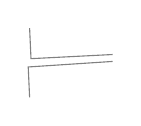
\begin{tikzpicture}[x=1em,y=1em]\draw[gray] (0,1.5)--(.05,.4)--(3,.55);\draw[gray] (0,-1)--(-.05,.1)--(3,.3);\end{tikzpicture}}}intervals being the obvious one).  No\var{\over{w}{w}}{\hand{w}}{writing over}{ps_134-4_023-v0017} here's the organigram:

\margin{(D)}
\diagram{
% Hand-drawn arrows are marked blue; typed objects remain plain.
\begin{tikzcd}[arrows=Rightarrow, column sep=huge, row sep=large]
\begin{array}{l}\text{1\hand{)} homotopy relation}\\ R_h\hand{\ensuremath{\subset}}\mathrm F\var{\over{l}{l}}{\hand{l}}{writing over}{ps_134-4_023-v0018}(M)\mathrm{x}\mathrm F\var{\over{l}{l}}{\hand{l}}{writing over}{ps_134-4_023-v0019}(M)\end{array}
  \ar[color=blue,r] \ar[color=blue,d] \&
\begin{array}{l}\text{2\hand{)} homotopisms}\\ W_h\hand{\ensuremath{\subset}}\mathrm F\var{\over{l}{l}}{\hand{l}}{writing over}{ps_134-4_023-v0020}(M)\end{array}
  \ar[color=blue,l, bend right=15, dashed, swap, "\hand{1}"] \ar[color=blue,d] \\
\begin{array}{l}\text{3\hand{)} homotopy intervals}\\ \hand{\ensuremath{\Sigma}}_h\hand{\ensuremath{\subset}}\mathrm{Int}(M)\end{array}
  \ar[color=blue,u, bend left=30, dashed, "\hand{2}"] \&
\begin{array}{l}\text{4\hand{)} contractible objects}\\ C_h\hand{\ensuremath{\subset}}\mathrm{Ob}(M)\end{array}
  \ar[color=blue,l, dashed, swap, "\hand{3}"]
\end{tikzcd}
}
\margin{\diagram{\begin{tikzpicture}[x=1em,y=1em]\node at (0,0) {$\ast$};\draw[line width=.6pt](-.2,-1.5)--(.2,-1.7);\end{tikzpicture}}}

\margin{23}

%% END SOURCE ps_134-4_023
\ifnum\EditionMode=1
\psapparatusstart
\psentry{ps_134-4_023-v0001}{1}{typewriter overwriting}{\over[typed]{n}{n}}{n}{The superposed typed reading replaces the underlying reading.}
\psentry{ps_134-4_023-v0002}{2}{typewriter overwriting}{\over[typed]{o}{o}}{o}{The superposed typed reading replaces the underlying reading.}
\psentry{ps_134-4_023-v0003}{3}{typewriter overwriting}{\over[typed]{\unsure{u}}{i}}{i}{The superposed typed reading replaces the underlying reading.}
\psentry{ps_134-4_023-v0004}{4}{typewriter overwriting}{\over[typed]{h}{h}}{h}{The superposed typed reading replaces the underlying reading.}
\psentry{ps_134-4_023-v0005}{5}{typewriter overwriting}{\over[typed]{h}{h}}{h}{The superposed typed reading replaces the underlying reading.}
\psentry{ps_134-4_023-v0006}{6}{typed insertion}{\inserted[typed]{homotopy}}{homotopy}{The typed insertion is incorporated at its indicated position; insertion brackets leave the running text.}
\psentry{ps_134-4_023-v0007}{7}{author join applied}{technic\hand{\ensuremath{\smile}}al}{technical}{The visible pen curve joins the two parts of technical.}
\psentry{ps_134-4_023-v0008}{8}{insertion}{\inserted{at will}}{\hand{at will}}{The handwritten insertion is incorporated at its indicated position; insertion brackets leave the running text.}
\psentry{ps_134-4_023-v0009}{9}{slip corrected}{relationsships}{relationships}{One-off extra s; relationships is correctly attested on reviewed ps\_134-3\_036.}
\psentry{ps_134-4_023-v0010}{10}{typewriter deletion}{\xout{expressed}}{}{The typewriter strikes out this material; it leaves the corrected running text.}
\psentry{ps_134-4_023-v0011}{11}{typewriter overwriting}{\over[typed]{\unsure{f}}{c}}{c}{The superposed typed reading replaces the underlying reading.}
\psentry{ps_134-4_023-v0012}{12}{deletion}{$\deleted{\unsure{M}}$}{}{The author cancels this material by hand; it leaves the corrected running text.}
\psentry{ps_134-4_023-v0013}{13}{typewriter overwriting}{\over[typed]{\unsure{j}}{t}}{t}{The superposed typed reading replaces the underlying reading.}
\psentry{ps_134-4_023-v0014}{14}{typewriter overwriting}{\over[typed]{m}{m}}{m}{The superposed typed reading replaces the underlying reading.}
\psentry{ps_134-4_023-v0015}{15}{writing over}{\over{e}{e}}{\hand{e}}{The superposed handwritten reading replaces the underlying reading.}
\psentry{ps_134-4_023-v0016}{16}{typewriter overwriting}{\over[typed]{N}{n}}{n}{The superposed typed reading replaces the underlying reading.}
\psentry{ps_134-4_023-v0017}{17}{writing over}{\over{w}{w}}{\hand{w}}{The superposed handwritten reading replaces the underlying reading.}
\psentry{ps_134-4_023-v0018}{18}{writing over}{$\over{l}{l}$}{$\hand{l}$}{The superposed handwritten reading replaces the underlying reading.}
\psentry{ps_134-4_023-v0019}{19}{writing over}{$\over{l}{l}$}{$\hand{l}$}{The superposed handwritten reading replaces the underlying reading.}
\psentry{ps_134-4_023-v0020}{20}{writing over}{$\over{l}{l}$}{$\hand{l}$}{The superposed handwritten reading replaces the underlying reading.}
\psapparatusend
\fi
\pssource{ps_134-4_024}{134-4/24}{https://grothendieck.umontpellier.fr/web/viewer.html?file=../134-4.pdf\#page=25}
\psnumber{ps_134-4_024-v0001}{1}
\psnumber{ps_134-4_024-v0002}{2}
\psnumber{ps_134-4_024-v0003}{3}
\psnumber{ps_134-4_024-v0004}{4}
\psnumber{ps_134-4_024-v0005}{5}
\psnumber{ps_134-4_024-v0006}{6}
\psnumber{ps_134-4_024-v0007}{7}
\psnumber{ps_134-4_024-v0008}{8}
\psnumber{ps_134-4_024-v0009}{9}
\psnumber{ps_134-4_024-v0010}{10}
\psnumber{ps_134-4_024-v0011}{11}
\psnumber{ps_134-4_024-v0012}{12}
\psnumber{ps_134-4_024-v0013}{13}
\psnumber{ps_134-4_024-v0014}{14}
\psnumber{ps_134-4_024-v0015}{15}
\psnumber{ps_134-4_024-v0016}{16}
\psnumber{ps_134-4_024-v0017}{17}
%% BEGIN SOURCE ps_134-4_024
% Pursuing Stacks (cotes 134-2 to 134-8): archive cote 134-4, site page 24 (PDF page 25), typescript page 112.
% typescript. Draft compared: ps3.tex:1177-1245.
% AI-transcribed by Claude Opus 5.5 (claude-opus-5-5, adaptive thinking, effort high), Message Batches API, batch ps2 (msgbatch_01NVwr1Yuo8qJf5rykeGBXPK), 2026-11-12; image review recorded in records/CHECK_DECISIONS_134_3_4.tsv.
\scanpage{134-4/24}
\mspage{112}

A) \uline{Homotopy relation between maps}. As a \uline{type of structure}, a
homotopy relation between maps in M is a subset
\[ R_h \hand{\subset} \mathrm F\var{\over{l}{l}}{\hand{l}}{writing over}{ps_134-4_024-v0001}(M)\mathrm{x}\mathrm F\var{\over{l}{l}}{\hand{l}}{writing over}{ps_134-4_024-v0002}(M) \]
namely a relation in the set $\mathrm F\var{\over{l}{l}}{\hand{l}}{writing over}{ps_134-4_024-v0003}(M)$ \var{or arrows of M}{of arrows of M}{slip corrected}{ps_134-4_024-v0004} , the \uline{basic assumption}
being that whenever f and g are \hand{``}homotopic\hand{''} arrows, then they have same
source, and same target. Thus the data $R_h$ is equivalent to giving a
``homotopy relation'' in any one of the sets Hom(X,Y), with X and Y objects
in M. T\var{\over{H}{h}}{\hand{h}}{writing over}{ps_134-4_024-v0005}e relevant \uline{saturation condition} is twofold:

a) \var{\over[typed]{T}{T}}{T}{typewriter overwriting}{ps_134-4_024-v0006}he relation $R_h$ is an equivalence relation, or equivalently, the
corresponding relations in the sets Hom(X,Y) are \var{equivalehce}{equivalence}{slip corrected}{ps_134-4_024-v0007} relations;

b) stability under composition: if f and g are homotopic, then so
are vf and vg , and so are fu and gu , for any arrow v or u such that
the relation makes sense.

When these conditions are satisfied, we'll say we got a \uline{homotopy}
\uline{relation} \var{\xout{on M}}{}{typewriter deletion}{ps_134-4_024-v0008} between maps of M. This relation \var{\inserted[typed]{between f and g}}{between f and g}{typed insertion}{ps_134-4_024-v0009} will be denoted by a sym-%
bol like
\[ f \underset{h}{\hand{\sim}} g \qquad . \]
If the basic assumption is satisfied, but not the saturation condition,
there is an evident way of ``saturating'' the given relation, getting
\var{\deleted{a saturated}}{}{deletion}{ps_134-4_024-v0010} one $\overset{\hand{\rule{0.65em}{0.4pt}}}{R}_h$ which is saturated i.e. a homotopy relation in M
(in fact, the smallest one containing $R_h$).

Given a homotopy relation $R_h$ , we denote by \var{\xout{Hom}}{}{typewriter deletion}{ps_134-4_024-v0011}
\[ \mathrm{Hom}(X,Y)_h \]
the corresponding quotient sets of the sets Hom(X,Y), they compose in an
evident way, so as to give rise to a \var{\xout{functor}}{}{typewriter deletion}{ps_134-4_024-v0012} category $M_h$ having same
objects as M, and to a canonical functor
\[ M \hand{\longrightarrow} M_h \]
which is the identity on objects, and surjective on arrows. We may
view thus $M_h$ as a \uline{quotient category} of M, having same objects as M.
Clearly, $R_h \hand{\longmapsto} M_h$ is a bijective correspondance between \var{\over[typed]{t}{t}}{t}{typewriter overwriting}{ps_134-4_024-v0013}he set of homo-%
topy relations in M, and the set of quotient categories of M satisfying
the aforesaid property. By abuse of language, we may even consider that
considering a homotopy relation in $\underset{\hand{\unsure{\cdot}}}{M}$, amounts to the same as giving a
functor $M \hand{\rightarrow} M_h$ \var{\inserted{from M}}{\hand{from M}}{insertion}{ps_134-4_024-v0014} which is bijective on objects and surjective on arrows.

When we got a homotopy relation $R_h$ in M, we deduce a notion of
\uline{homotopisms}
\[ W_h \hand{\subset} \mathrm F\var{\over{l}{l}}{\hand{l}}{writing over}{ps_134-4_024-v0015}(M) \ , \]
namely those arrows in M which \var{\deleted{\xout{\unsure{are}}}}{}{deletion}{ps_134-4_024-v0016} become isomorphisms in $M_{\var{\over{\illegible{1}}{h}}{\hand{h}}{writing over}{ps_134-4_024-v0017}}$ . Also we

\margin{24}

%% END SOURCE ps_134-4_024
\ifnum\EditionMode=1
\psapparatusstart
\psentry{ps_134-4_024-v0001}{1}{writing over}{$\over{l}{l}$}{$\hand{l}$}{The superposed handwritten reading replaces the underlying reading.}
\psentry{ps_134-4_024-v0002}{2}{writing over}{$\over{l}{l}$}{$\hand{l}$}{The superposed handwritten reading replaces the underlying reading.}
\psentry{ps_134-4_024-v0003}{3}{writing over}{$\over{l}{l}$}{$\hand{l}$}{The superposed handwritten reading replaces the underlying reading.}
\psentry{ps_134-4_024-v0004}{4}{slip corrected}{or arrows of M}{of arrows of M}{One-off r for f in the definition of the set of arrows; of is correctly attested on the same page.}
\psentry{ps_134-4_024-v0005}{5}{writing over}{\over{H}{h}}{\hand{h}}{The superposed handwritten reading replaces the underlying reading.}
\psentry{ps_134-4_024-v0006}{6}{typewriter overwriting}{\over[typed]{T}{T}}{T}{The superposed typed reading replaces the underlying reading.}
\psentry{ps_134-4_024-v0007}{7}{slip corrected}{equivalehce}{equivalence}{One-off h for n; equivalence is correctly typed in the preceding line.}
\psentry{ps_134-4_024-v0008}{8}{typewriter deletion}{\xout{on M}}{}{The typewriter strikes out this material; it leaves the corrected running text.}
\psentry{ps_134-4_024-v0009}{9}{typed insertion}{\inserted[typed]{between f and g}}{between f and g}{The typed insertion is incorporated at its indicated position; insertion brackets leave the running text.}
\psentry{ps_134-4_024-v0010}{10}{deletion}{\deleted{a saturated}}{}{The author cancels this material by hand; it leaves the corrected running text.}
\psentry{ps_134-4_024-v0011}{11}{typewriter deletion}{\xout{Hom}}{}{The typewriter strikes out this material; it leaves the corrected running text.}
\psentry{ps_134-4_024-v0012}{12}{typewriter deletion}{\xout{functor}}{}{The typewriter strikes out this material; it leaves the corrected running text.}
\psentry{ps_134-4_024-v0013}{13}{typewriter overwriting}{\over[typed]{t}{t}}{t}{The superposed typed reading replaces the underlying reading.}
\psentry{ps_134-4_024-v0014}{14}{insertion}{\inserted{from M}}{\hand{from M}}{The handwritten insertion is incorporated at its indicated position; insertion brackets leave the running text.}
\psentry{ps_134-4_024-v0015}{15}{writing over}{$\over{l}{l}$}{$\hand{l}$}{The superposed handwritten reading replaces the underlying reading.}
\psentry{ps_134-4_024-v0016}{16}{deletion}{\deleted{\xout{\unsure{are}}}}{}{The author cancels this material by hand; it leaves the corrected running text.}
\psentry{ps_134-4_024-v0017}{17}{writing over}{$\over{\illegible{1}}{h}$}{$\hand{h}$}{The superposed handwritten reading replaces the underlying reading.}
\psapparatusend
\fi
\pssource{ps_134-4_025}{134-4/25}{https://grothendieck.umontpellier.fr/web/viewer.html?file=../134-4.pdf\#page=26}
\psnumber{ps_134-4_025-v0001}{1}
\psnumber{ps_134-4_025-v0002}{2}
\psnumber{ps_134-4_025-v0003}{3}
\psnumber{ps_134-4_025-v0004}{4}
\psnumber{ps_134-4_025-v0005}{5}
\psnumber{ps_134-4_025-v0006}{6}
\psnumber{ps_134-4_025-v0007}{7}
\psnumber{ps_134-4_025-v0008}{8}
\psnumber{ps_134-4_025-v0009}{9}
\psnumber{ps_134-4_025-v0010}{10}
\psnumber{ps_134-4_025-v0011}{11}
\psnumber{ps_134-4_025-v0012}{12}
\psnumber{ps_134-4_025-v0013}{13}
\psnumber{ps_134-4_025-v0014}{14}
\psnumber{ps_134-4_025-v0015}{15}
\psnumber{ps_134-4_025-v0016}{16}
\psnumber{ps_134-4_025-v0017}{17}
\psnumber{ps_134-4_025-v0018}{18}
%% BEGIN SOURCE ps_134-4_025
% Pursuing Stacks (cotes 134-2 to 134-8): archive cote 134-4, site page 25 (PDF page 26), typescript page 113.
% typescript. Draft compared: ps3.tex:1229-1293.
% AI-transcribed by Claude Opus 5.5 (claude-opus-5-5, adaptive thinking, effort high), Message Batches API, batch ps2 (msgbatch_01NVwr1Yuo8qJf5rykeGBXPK), 2026-11-12; image review recorded in records/CHECK_DECISIONS_134_3_4.tsv.
\scanpage{134-4/25}
\mspage{113}
deduce a notion of \uline{homotopy interval}  i.e.
\[ \hand{\Sigma}_h \hand{\subset} \mathrm{Int}(M) \quad , \]
% NOTE: the right edge of the scan is cut; words at the end of some lines are incomplete (homoto..., ca..., commute...)
namely those intervals $\underline{I}$ in M such that the  two marked sections be homoto%
pic. (NB $\hand{\Sigma}_h$ is non empty if and only if M has a final element,  in this ca%
se $\var{\over{\illegible{1}}{\Sigma}}{\hand{\Sigma}}{writing over}{ps_134-4_025-v0001}_{\hand{h}}$ contains all intervals such that $\hand{\delta}_o=\hand{\delta}_1$  -  which we may call \uline{trivial}
intervals,  for instance the \uline{final interval} with I=\hand{e}...)  This notion of
a homotopy interval is considerably wider than the one we have worked with
so far,  however it is clearly the right one in the context of \var{\inserted[typed]{pure}}{pure}{typed insertion}{ps_134-4_025-v0002} homotopy
notions.  To avoid any confusion,  we better call this notion by the name
of \uline{weak} \uline{homotopy} \uline{intervals}  -  funnily there won't be any unqualified
\hand{``}homotopy intervals\hand{''} in our present set-up of ``pure'' homotopy notions !

T\var{\over[typed]{H}{h}}{h}{typewriter overwriting}{ps_134-4_025-v0003}e two prescriptions  above account for \var{twp  among}{two  among}{slip corrected}{ps_134-4_025-v0004} the plain arrows
in our organigram.

\var{\deleted{\illegible{1}}}{}{deletion}{ps_134-4_025-v0005}We'll often make use of an \uline{accessory assumption} on R$_h$ ,  which \var{\over[typed]{i}{c}}{c}{typewriter overwriting}{ps_134-4_025-v0006}\var{\over[typed]{a}{a}}{a}{typewriter overwriting}{ps_134-4_025-v0007}n
be expressed by demanding that \uline{the canonical functor} M$\hand{\to}$ M$_h$  \uline{commute} \uline{to}
\uline{binary products},  in case we assume already such products exist in M.
This can be expressed also by the property that for two maps
\[ f,g \ :\ X \hand{\rightrightarrows} Y_1 x Y_2 \quad , \]
f and g are homotopic iff  so are f$_i$ and g$_i$  ($i\hand{\in\{}1,2\hand{\}}$)  (where the ``only
if'' part is satisfied \var{\xout{anyhow}}{}{typewriter deletion}{ps_134-4_025-v0008} beforehand anyhow).  This implie\var{\over{s}{s}}{\hand{s}}{writing over}{ps_134-4_025-v0009} \var{\inserted[typed]{too}}{too}{typed insertion}{ps_134-4_025-v0010} that in
M$_h$ binary products exist\hand{,} \var{\inserted{and that $f\sim f', g\sim g'$ implies $f\times g\sim f'\times g'$.}}{\hand{and that $f\sim f', g\sim g'$ implies $f\times g\sim f'\times g'$.}}{insertion}{ps_134-4_025-v0011} \var{\deleted{and}}{}{deletion}{ps_134-4_025-v0012} \unsure{that} On the other hand,  it is trivial that
if M admits a final object,  this is equally a final object of M$_h$  (and
hence,  under the accessory assumption on R$_h$ ,  the functor M$\hand{\to}$M$_h$ commutes
to finite products).

B)  \uline{Homotopisms}.  As a type of structure on M, we got just a subset
\[ W_h \hand{\subset} \mathrm F\var{\over{l}{l}}{\hand{l}}{writing over}{ps_134-4_025-v0013}(M) \quad , \]
without any basic assumption to make.  T\unsure{\var{\over[typed]{H}{h}}{h}{typewriter overwriting}{ps_134-4_025-v0014}}e natural \uline{saturation condition}
is just the strong saturation for a subset of F\var{\over{l}{l}}{\hand{l}}{writing over}{ps_134-4_025-v0015}(M),  which can be expres-%
sed by stating that W$_h$ can be obtained as the set of arrows made invertib-%
le by some functor from M into a category M',  or equivalently,  by the
localisation functor
\[ \hand{M}\var{\over{M}{\to}}{\hand{\to}}{writing over}{ps_134-4_025-v0016} \var{\deleted{\illegible{1}}}{}{deletion}{ps_134-4_025-v0017} W_h^{-1}M \var{\deleted{\illegible{1}}}{}{deletion}{ps_134-4_025-v0018} \hand{.} \]
We may refer to a strongly saturated W$_h$ as a ``\uline{homotopism} \uline{structure}''
(or ``homotopy equivalence structure'') in M  -  but as in the case A),
we'll have soon enough to make pretty strong extra assumptions.  Maybe
we should, at the very least,  demand for the notion of homotopy structure
that the canonical functor above,  which is bijective on objects in any
case,  should be moreover \uline{surjective on arrows}  -  thus I'll take this

\margin{25}

%% END SOURCE ps_134-4_025
\ifnum\EditionMode=1
\psapparatusstart
\psentry{ps_134-4_025-v0001}{1}{writing over}{$\over{\illegible{1}}{\Sigma}$}{$\hand{\Sigma}$}{The superposed handwritten reading replaces the underlying reading.}
\psentry{ps_134-4_025-v0002}{2}{typed insertion}{\inserted[typed]{pure}}{pure}{The typed insertion is incorporated at its indicated position; insertion brackets leave the running text.}
\psentry{ps_134-4_025-v0003}{3}{typewriter overwriting}{\over[typed]{H}{h}}{h}{The superposed typed reading replaces the underlying reading.}
\psentry{ps_134-4_025-v0004}{4}{slip corrected}{twp  among}{two  among}{One-off p for o, with two correctly typed at the beginning of the same sentence.}
\psentry{ps_134-4_025-v0005}{5}{deletion}{\deleted{\illegible{1}}}{}{The author cancels this material by hand; it leaves the corrected running text.}
\psentry{ps_134-4_025-v0006}{6}{typewriter overwriting}{\over[typed]{i}{c}}{c}{The superposed typed reading replaces the underlying reading.}
\psentry{ps_134-4_025-v0007}{7}{typewriter overwriting}{\over[typed]{a}{a}}{a}{The superposed typed reading replaces the underlying reading.}
\psentry{ps_134-4_025-v0008}{8}{typewriter deletion}{\xout{anyhow}}{}{The typewriter strikes out this material; it leaves the corrected running text.}
\psentry{ps_134-4_025-v0009}{9}{writing over}{\over{s}{s}}{\hand{s}}{The superposed handwritten reading replaces the underlying reading.}
\psentry{ps_134-4_025-v0010}{10}{typed insertion}{\inserted[typed]{too}}{too}{The typed insertion is incorporated at its indicated position; insertion brackets leave the running text.}
\psentry{ps_134-4_025-v0011}{11}{insertion}{\inserted{and that $f\sim f', g\sim g'$ implies $f\times g\sim f'\times g'$.}}{\hand{and that $f\sim f', g\sim g'$ implies $f\times g\sim f'\times g'$.}}{The handwritten insertion is incorporated at its indicated position; insertion brackets leave the running text.}
\psentry{ps_134-4_025-v0012}{12}{deletion}{\deleted{and}}{}{The author cancels this material by hand; it leaves the corrected running text.}
\psentry{ps_134-4_025-v0013}{13}{writing over}{$\over{l}{l}$}{$\hand{l}$}{The superposed handwritten reading replaces the underlying reading.}
\psentry{ps_134-4_025-v0014}{14}{typewriter overwriting}{\over[typed]{H}{h}}{h}{The superposed typed reading replaces the underlying reading.}
\psentry{ps_134-4_025-v0015}{15}{writing over}{\over{l}{l}}{\hand{l}}{The superposed handwritten reading replaces the underlying reading.}
\psentry{ps_134-4_025-v0016}{16}{writing over}{$\over{M}{\to}$}{$\hand{\to}$}{The superposed handwritten reading replaces the underlying reading.}
\psentry{ps_134-4_025-v0017}{17}{deletion}{$\deleted{\illegible{1}}$}{}{The author cancels this material by hand; it leaves the corrected running text.}
\psentry{ps_134-4_025-v0018}{18}{deletion}{$\deleted{\illegible{1}}$}{}{The author cancels this material by hand; it leaves the corrected running text.}
\psapparatusend
\fi
\pssource{ps_134-4_026}{134-4/26}{https://grothendieck.umontpellier.fr/web/viewer.html?file=../134-4.pdf\#page=27}
\psnumber{ps_134-4_026-v0001}{1}
\psnumber{ps_134-4_026-v0002}{2}
\psnumber{ps_134-4_026-v0003}{3}
\psnumber{ps_134-4_026-v0004}{4}
\psnumber{ps_134-4_026-v0005}{5}
\psnumber{ps_134-4_026-v0006}{6}
\psnumber{ps_134-4_026-v0007}{7}
\psnumber{ps_134-4_026-v0008}{8}
\psnumber{ps_134-4_026-v0009}{9}
\psnumber{ps_134-4_026-v0010}{10}
\psnumber{ps_134-4_026-v0011}{11}
\psnumber{ps_134-4_026-v0012}{12}
\psnumber{ps_134-4_026-v0013}{13}
\psnumber{ps_134-4_026-v0014}{14}
\psnumber{ps_134-4_026-v0015}{15}
\psnumber{ps_134-4_026-v0016}{16}
\psnumber{ps_134-4_026-v0017}{17}
\psnumber{ps_134-4_026-v0018}{18}
\psnumber{ps_134-4_026-v0019}{19}
\psnumber{ps_134-4_026-v0020}{20}
\psnumber{ps_134-4_026-v0021}{21}
\psnumber{ps_134-4_026-v0022}{22}
\psnumber{ps_134-4_026-v0023}{23}
\psnumber{ps_134-4_026-v0024}{24}
\psnumber{ps_134-4_026-v0025}{25}
\psnumber{ps_134-4_026-v0026}{26}
\psnumber{ps_134-4_026-v0027}{27}
\psnumber{ps_134-4_026-v0028}{28}
\psnumber{ps_134-4_026-v0029}{29}
\psnumber{ps_134-4_026-v0030}{30}
\psnumber{ps_134-4_026-v0031}{31}
%% BEGIN SOURCE ps_134-4_026
% Pursuing Stacks (cotes 134-2 to 134-8): archive cote 134-4, site page 26 (PDF page 27), typescript page 114.
% typescript. Draft compared: ps3.tex:1281-1345.
% AI-transcribed by Claude Opus 5.5 (claude-opus-5-5, adaptive thinking, effort high), Message Batches API, batch ps2 (msgbatch_01NVwr1Yuo8qJf5rykeGBXPK), 2026-11-12; image review recorded in records/CHECK_DECISIONS_134_3_4.tsv.
\scanpage{134-4/26}
\mspage{114}

as a \uline{basic assumption} after all.  This assumption makes sense of course
independently of any saturation condition.  If $W_h$ is not \var{\xout{\unsure{satura}}}{}{typewriter deletion}{ps_134-4_026-v0001} strongly
saturated,  then denoting by $\overset{\hand{\rule{0.6em}{0.4pt}}}{W}_h$ the subset of $F\var{\over{l}{l}}{\hand{l}}{writing over}{ps_134-4_026-v0002}(M)$ of all arrows made
invertible by the canonical functor,  this will now be a strongly satura-%
ted set of arrows (in fact the smallest one containing $\var{\over{W}{W}}{\hand{W}}{writing over}{ps_134-4_026-v0003}_h$\var{\deleted{)}}{}{deletion}{ps_134-4_026-v0004},  and giving
rise to the same localise\var{\over[typed]{\illegible{1}}{d}}{d}{typewriter overwriting}{ps_134-4_026-v0005} category,  and hence satisfying the basic \var{\xout{\unsure{assum}}}{}{typewriter deletion}{ps_134-4_026-v0006}
\var{assuption too}{assumption too}{slip corrected}{ps_134-4_026-v0007}\hand{)} -  thus $\overset{\hand{\rule{0.6em}{0.4pt}}}{W}_h$ is indeed a homotopism structure on M.

When M admits a final object,  this will equally be a final object of
$W_h^{-1}M$ . We may now define in terms of $W_h$  the notion of contractible
\var{\xout{elements}}{}{typewriter deletion}{ps_134-4_026-v0008} objects in M , \var{\over{\illegible{1}}{forming}}{\hand{forming}}{writing over}{ps_134-4_026-v0009} a subset
\[ C_h \hand{\subset} Ob(M) \quad , \]
as those objects X in M such that  the projection $p_X : X \hand{\ensuremath{\to}} e$ is in $W_h$ ,
or , equivalently,  such that X is \var{\xout{isomorphic}}{}{typewriter deletion}{ps_134-4_026-v0010} a final object in the loca-%
lized category $W_h^{-1}M$ .  This accounts for the th\var{\over{\unsure{ri}}{ir}}{\hand{ir}}{writing over}{ps_134-4_026-v0011}d plain arrow of the
\var{\uline{organigram.}\diagram{\begin{tikzpicture}[baseline=-0.4ex,x=1em,y=1ex]\draw (0,0)--(0.4,0)--(0.4,1.6)--(1.8,1.6);\end{tikzpicture}}}{\uline{organigram.}\par}{author paragraph instruction}{ps_134-4_026-v0012} We'll now \var{\xout{\illegible{1}}}{}{typewriter deletion}{ps_134-4_026-v0013}\var{\inserted{dwell}}{\hand{dwell}}{insertion}{ps_134-4_026-v0014} a little more on the first dotted arrow,
namely the description of a homotopy relation
\[ R_h \hand{\subset} F\var{\over{l}{l}}{\hand{l}}{writing over}{ps_134-4_026-v0015}(M)\mathrm{x}F\var{\over{l}{l}}{\hand{l}}{writing over}{ps_134-4_026-v0016}(M) \]
in terms of $W_h$ :  \var{\over{T}{t}}{\hand{t}}{writing over}{ps_134-4_026-v0017}\var{\over[typed]{H}{h}}{h}{typewriter overwriting}{ps_134-4_026-v0018}e natural choice here is to define  f,g\hand{$\in$} \var{\xout{xxxxx}}{}{typewriter deletion}{ps_134-4_026-v0019}\var{\inserted[typed]{$F\over{l}{l}(M)$}}{$F\hand{l}(M)$}{typed insertion}{ps_134-4_026-v0020} to
be \uline{homotopic} (\uline{or $W_h$}-homotopic, if ambiguity may arise)  iff their images
in the category $W_h^{-1}M$  are equa\var{\over{\illegible{1}}{l}}{\hand{l}}{writing over}{ps_134-4_026-v0021}.  This \var{\xout{homotopy notion}}{}{typewriter deletion}{ps_134-4_026-v0022}\var{\inserted[typed]{relation}}{relation}{typed insertion}{ps_134-4_026-v0023} between maps
in M clearly satisfies the basic assumption on source and target,  as well
as the saturation condition  -  it is  therefore a``homotopy \var{\over{\illegible{1}}{rela}}{\hand{rela}}{writing over}{ps_134-4_026-v0024}tion'' in M,
\var{\xout{and}}{}{typewriter deletion}{ps_134-4_026-v0025} namely the one associated to $\var{\over{W}{W}}{\hand{W}}{writing over}{ps_134-4_026-v0026}_h$\hand{$^{-1}M$,} viewed as a quotient category of M.
It is clear that we recover $W_h$ from $R_h$ ,  consequently,  by the process
described in A),  \var{\xout{of taking}}{}{typewriter deletion}{ps_134-4_026-v0027}

To make the relationship between the notions 1\hand{)} and 2\hand{)} still clearer,
let\hand{'}s denote respectively by
\[ Ho\var{\over[typed]{M}{m}}{m}{typewriter overwriting}{ps_134-4_026-v0028}_1(M),\ Hom_2(M) \]
the set of all homotopy \var{\xout{\unsure{notions resp.}}}{}{typewriter deletion}{ps_134-4_026-v0029} relations,  resp. of all homotopism
notions,  in M.  We got maps\hand{*}
% Hand-drawn arrows are marked blue; typed objects remain plain.
\diagram{\begin{tikzcd} Hom_1(M) \arrow[r, shift left, color=blue, "\hand{r_{21}}"] \& Hom_2(M) \arrow[l, shift left, color=blue, "\hand{r_{12}}"] \end{tikzcd} \quad ,}
\margin{* 3.4. There \uline{is no} \uline{map} $r_{21}$, only $r_{12}$, see correction in \S\ 51!}
and the relevant fact here is that
\[ r_{12}: Hom_2 \hand{\ensuremath{\longrightarrow}} Hom_1 \]
\uline{is injective},  \uline{and admits} $r_{21}$ \uline{as a left inverse}.  Thus we may view
$Hom_2$ as a subset of $Hom_1$ ,  i.e. the structure of a ``homotopism notion'' on
M as a particular case of the structure of a ``homotopy relation'' on M.
Namely,  a structure of the latter type can be described in terms of a
notion of homotopism in M,  iff the canonical functor $M \hand{\ensuremath{\to}} M_h$ i\var{\over{s}{t}}{\hand{t}}{writing over}{ps_134-4_026-v0030} gives rise
\var{\xout{to}}{}{typewriter deletion}{ps_134-4_026-v0031}

\margin{26}

%% END SOURCE ps_134-4_026
\ifnum\EditionMode=1
\psapparatusstart
\psentry{ps_134-4_026-v0001}{1}{typewriter deletion}{\xout{\unsure{satura}}}{}{The typewriter strikes out this material; it leaves the corrected running text.}
\psentry{ps_134-4_026-v0002}{2}{writing over}{$\over{l}{l}$}{$\hand{l}$}{The superposed handwritten reading replaces the underlying reading.}
\psentry{ps_134-4_026-v0003}{3}{writing over}{$\over{W}{W}$}{$\hand{W}$}{The superposed handwritten reading replaces the underlying reading.}
\psentry{ps_134-4_026-v0004}{4}{deletion}{\deleted{)}}{}{The author cancels this material by hand; it leaves the corrected running text.}
\psentry{ps_134-4_026-v0005}{5}{typewriter overwriting}{\over[typed]{\illegible{1}}{d}}{d}{The superposed typed reading replaces the underlying reading.}
\psentry{ps_134-4_026-v0006}{6}{typewriter deletion}{\xout{\unsure{assum}}}{}{The typewriter strikes out this material; it leaves the corrected running text.}
\psentry{ps_134-4_026-v0007}{7}{slip corrected}{assuption too}{assumption too}{An isolated missing m, settled by correctly typed assumption twice on the same page.}
\psentry{ps_134-4_026-v0008}{8}{typewriter deletion}{\xout{elements}}{}{The typewriter strikes out this material; it leaves the corrected running text.}
\psentry{ps_134-4_026-v0009}{9}{writing over}{\over{\illegible{1}}{forming}}{\hand{forming}}{The superposed handwritten reading replaces the underlying reading.}
\psentry{ps_134-4_026-v0010}{10}{typewriter deletion}{\xout{isomorphic}}{}{The typewriter strikes out this material; it leaves the corrected running text.}
\psentry{ps_134-4_026-v0011}{11}{writing over}{\over{\unsure{ri}}{ir}}{\hand{ir}}{The superposed handwritten reading replaces the underlying reading.}
\psentry{ps_134-4_026-v0012}{12}{author paragraph instruction}{\uline{organigram.}\diagram{\begin{tikzpicture}[baseline=-0.4ex,x=1em,y=1ex]\draw (0,0)--(0.4,0)--(0.4,1.6)--(1.8,1.6);\end{tikzpicture}}}{\uline{organigram.}\par}{The author draws a step between organigram and We'll now to begin a new paragraph.}
\psentry{ps_134-4_026-v0013}{13}{typewriter deletion}{\xout{\illegible{1}}}{}{The typewriter strikes out this material; it leaves the corrected running text.}
\psentry{ps_134-4_026-v0014}{14}{insertion}{\inserted{dwell}}{\hand{dwell}}{The handwritten insertion is incorporated at its indicated position; insertion brackets leave the running text.}
\psentry{ps_134-4_026-v0015}{15}{writing over}{$\over{l}{l}$}{$\hand{l}$}{The superposed handwritten reading replaces the underlying reading.}
\psentry{ps_134-4_026-v0016}{16}{writing over}{$\over{l}{l}$}{$\hand{l}$}{The superposed handwritten reading replaces the underlying reading.}
\psentry{ps_134-4_026-v0017}{17}{writing over}{\over{T}{t}}{\hand{t}}{The superposed handwritten reading replaces the underlying reading.}
\psentry{ps_134-4_026-v0018}{18}{typewriter overwriting}{\over[typed]{H}{h}}{h}{The superposed typed reading replaces the underlying reading.}
\psentry{ps_134-4_026-v0019}{19}{typewriter deletion}{\xout{xxxxx}}{}{The typewriter strikes out this material; it leaves the corrected running text.}
\psentry{ps_134-4_026-v0020}{20}{typed insertion}{\inserted[typed]{$F\over{l}{l}(M)$}}{$F\hand{l}(M)$}{The typed insertion is incorporated at its indicated position; insertion brackets leave the running text.}
\psentry{ps_134-4_026-v0021}{21}{writing over}{\over{\illegible{1}}{l}}{\hand{l}}{The superposed handwritten reading replaces the underlying reading.}
\psentry{ps_134-4_026-v0022}{22}{typewriter deletion}{\xout{homotopy notion}}{}{The typewriter strikes out this material; it leaves the corrected running text.}
\psentry{ps_134-4_026-v0023}{23}{typed insertion}{\inserted[typed]{relation}}{relation}{The typed insertion is incorporated at its indicated position; insertion brackets leave the running text.}
\psentry{ps_134-4_026-v0024}{24}{writing over}{\over{\illegible{1}}{rela}}{\hand{rela}}{The superposed handwritten reading replaces the underlying reading.}
\psentry{ps_134-4_026-v0025}{25}{typewriter deletion}{\xout{and}}{}{The typewriter strikes out this material; it leaves the corrected running text.}
\psentry{ps_134-4_026-v0026}{26}{writing over}{$\over{W}{W}$}{$\hand{W}$}{The superposed handwritten reading replaces the underlying reading.}
\psentry{ps_134-4_026-v0027}{27}{typewriter deletion}{\xout{of taking}}{}{The typewriter strikes out this material; it leaves the corrected running text.}
\psentry{ps_134-4_026-v0028}{28}{typewriter overwriting}{$\over[typed]{M}{m}$}{$m$}{The superposed typed reading replaces the underlying reading.}
\psentry{ps_134-4_026-v0029}{29}{typewriter deletion}{\xout{\unsure{notions resp.}}}{}{The typewriter strikes out this material; it leaves the corrected running text.}
\psentry{ps_134-4_026-v0030}{30}{writing over}{\over{s}{t}}{\hand{t}}{The superposed handwritten reading replaces the underlying reading.}
\psentry{ps_134-4_026-v0031}{31}{typewriter deletion}{\xout{to}}{}{The typewriter strikes out this material; it leaves the corrected running text.}
\psapparatusend
\fi
\pssource{ps_134-4_027}{134-4/27}{https://grothendieck.umontpellier.fr/web/viewer.html?file=../134-4.pdf\#page=28}
\psnumber{ps_134-4_027-v0001}{1}
\psnumber{ps_134-4_027-v0002}{2}
\psnumber{ps_134-4_027-v0003}{3}
\psnumber{ps_134-4_027-v0004}{4}
\psnumber{ps_134-4_027-v0005}{5}
\psnumber{ps_134-4_027-v0006}{6}
\psnumber{ps_134-4_027-v0007}{7}
\psnumber{ps_134-4_027-v0008}{8}
\psnumber{ps_134-4_027-v0009}{9}
\psnumber{ps_134-4_027-v0010}{10}
\psnumber{ps_134-4_027-v0011}{11}
\psnumber{ps_134-4_027-v0012}{12}
\psnumber{ps_134-4_027-v0013}{13}
\psnumber{ps_134-4_027-v0014}{14}
\psnumber{ps_134-4_027-v0015}{15}
\psnumber{ps_134-4_027-v0016}{16}
\psnumber{ps_134-4_027-v0017}{17}
\psnumber{ps_134-4_027-v0018}{18}
%% BEGIN SOURCE ps_134-4_027
% Pursuing Stacks (cotes 134-2 to 134-8): archive cote 134-4, site page 27 (PDF page 28), typescript page 115.
% typescript. Draft compared: ps3.tex:1329-1392.
% AI-transcribed by Claude Opus 5.5 (claude-opus-5-5, adaptive thinking, effort high), Message Batches API, batch ps2 (msgbatch_01NVwr1Yuo8qJf5rykeGBXPK), 2026-11-12; image review recorded in records/CHECK_DECISIONS_134_3_4.tsv.
\scanpage{134-4/27}
\mspage{115}

\var{\inserted{to,}}{\hand{to,}}{insertion}{ps_134-4_027-v0001} is a localization functor.

\var{\xout{Here is a \uline{sufficient} condition on $R_h$ for an element $R_h$ of $\mathrm{Hom}_1$ to be}}{}{typewriter deletion}{ps_134-4_027-v0002}
\var{\xout{in the image of $\mathrm{Hom}_2$ , namely to be the}}{}{typewriter deletion}{ps_134-4_027-v0003}
For a general $R_h \hand{\in} \mathrm{Hom}_1(M)$ , if we consider the co\unsure{\var{\over[typed]{m}{r}}{r}{typewriter overwriting}{ps_134-4_027-v0004}}responding $W_h$
$( = r_{21}(R_h))$ in $\mathrm{Hom}_2(M)$, it is clear that the canonical functor $M \hand{\to} M_h$
of A factors into
\[ M \hand{\to} W_h^{-1}M \hand{\to} M_h \ , \]
and $R_h$ ``is in $\mathrm{Hom}_2(M)$'' i.e. $R_h = r_{12}(W_h)$, iff the second functor
\[ W_h^{-1}M \hand{\to} M_h \]
(which is anyhow bijective on objects and surjective on arrows) is an iso-%
morphism, or, equiv\var{\over{\unsure{alent}}{alent}}{\hand{alent}}{writing over}{ps_134-4_027-v0005}ly, faithful. Here is a rather evident \var{\deleted{\xout{\unsure{and}}}}{}{deletion}{ps_134-4_027-v0006}
\uline{sufficient} condition on $R_h$ for this to be so,\hand{$^*$} namely\hand{:}
\margin{* 3.4. See \S 52 for a \unsure{proof} of this rash statement!}
\var{\deleted{\xout{\unsure{(C}}}}{}{deletion}{ps_134-4_027-v0007} C$_{12}$) If $f,\var{\over{g}{g}}{\hand{g}}{writing over}{ps_134-4_027-v0008} : X \hand{\to} Y$ are homotopic, there exists a homotopism
$X' \hand{\to} X$ , \var{\deleted{and}}{}{deletion}{ps_134-4_027-v0009} two sections $s_o,s_1$ of $X'$ over $X$, and a map $h \colon X' \hand{\to} Y$ ,
such that
\[ f_o = hs_o \ , \ f_1 = hs_1 \ . \]
\uline{Remark.}Intuitively, we are thinking of course of $X'$ as a product $X\mathrm{x}I$ , where
$\underline{I} = (I,e_o,e_1)$ is a \var{\inserted{weak}}{\hand{weak}}{insertion}{ps_134-4_027-v0010} homotopy interval, and $s_o,s_1$ are defined in terms of
$e_o,e_1$ . In Quillen's somewhat different set-up, $X'$ is referred to as a
``cylinder object for $X$'' , suitable for defining the ``left homotopy rela-%
tion'' associated to a given $W_h$ . T\var{\over[typed]{H}{h}}{h}{typewriter overwriting}{ps_134-4_027-v0011}e condition C$_{12}$ is not autodual,
we could state a dual sufficient condition in terms of a ``path object for
$Y$ '', namely a homotopism $Y \hand{\to} Y'$ endowed with two retractions $t_o,t_1$ upon
$Y$ - but we won't have any use for this \var{\xout{xxx}}{}{typewriter deletion}{ps_134-4_027-v0012}\var{\inserted[typed]{in}}{in}{typed insertion}{ps_134-4_027-v0013} the present set up, which
(as far as the main emphasis is concerned) is by no means autodual, as
is Quillen's.

\margin{\unsure{$\cdot$}} T\var{\over[typed]{H}{h}}{h}{typewriter overwriting}{ps_134-4_027-v0014}e condition C$_{12}$ above can be viewed equally as a condition on
a $W_h \hand{\in} \mathrm{Hom}_2(M)$.

We may interprete the set $\mathrm{Hom}_2(M)$ of homotopism notions in $M$ as the
set of all quotient categories $M_h$ of $M$, having same \var{\xout{arrows}}{}{typewriter deletion}{ps_134-4_027-v0015} objects as $M$,
and such that moreover the canonical functor $M \hand{\to} M_h$ be a localizing func-%
tor . As in A), the relevant ``\uline{accessory assumption}'' on $W_h$ (a particular
case indeed of the corresponding one for $R_h$) is that th\var{\over[typed]{\illegible{1}}{i}}{i}{typewriter overwriting}{ps_134-4_027-v0016}s functor commute
to products. I dont see any \var{\xout{handy}}{}{typewriter deletion}{ps_134-4_027-v0017} simple computational way though to \var{\xout{expr}}{}{typewriter deletion}{ps_134-4_027-v0018}
express this condition directly in terms of $W_h$ , as previously in terms of
$R_h$. I would only like to notice here a consequence of this assumption
(I doubt it is equivalent to it), namely that \uline{the cartesian product of
two homotopisms is again a homotopism} - which implies, for instance,

\margin{27}

%% END SOURCE ps_134-4_027
\ifnum\EditionMode=1
\psapparatusstart
\psentry{ps_134-4_027-v0001}{1}{insertion}{\inserted{to,}}{\hand{to,}}{The handwritten insertion is incorporated at its indicated position; insertion brackets leave the running text.}
\psentry{ps_134-4_027-v0002}{2}{typewriter deletion}{\xout{Here is a \uline{sufficient} condition on $R_h$ for an element $R_h$ of $\mathrm{Hom}_1$ to be}}{}{The typewriter strikes out this material; it leaves the corrected running text.}
\psentry{ps_134-4_027-v0003}{3}{typewriter deletion}{\xout{in the image of $\mathrm{Hom}_2$ , namely to be the}}{}{The typewriter strikes out this material; it leaves the corrected running text.}
\psentry{ps_134-4_027-v0004}{4}{typewriter overwriting}{\over[typed]{m}{r}}{r}{The superposed typed reading replaces the underlying reading.}
\psentry{ps_134-4_027-v0005}{5}{writing over}{\over{\unsure{alent}}{alent}}{\hand{alent}}{The superposed handwritten reading replaces the underlying reading.}
\psentry{ps_134-4_027-v0006}{6}{deletion}{\deleted{\xout{\unsure{and}}}}{}{The author cancels this material by hand; it leaves the corrected running text.}
\psentry{ps_134-4_027-v0007}{7}{deletion}{\deleted{\xout{\unsure{(C}}}}{}{The author cancels this material by hand; it leaves the corrected running text.}
\psentry{ps_134-4_027-v0008}{8}{writing over}{$\over{g}{g}$}{$\hand{g}$}{The superposed handwritten reading replaces the underlying reading.}
\psentry{ps_134-4_027-v0009}{9}{deletion}{\deleted{and}}{}{The author cancels this material by hand; it leaves the corrected running text.}
\psentry{ps_134-4_027-v0010}{10}{insertion}{\inserted{weak}}{\hand{weak}}{The handwritten insertion is incorporated at its indicated position; insertion brackets leave the running text.}
\psentry{ps_134-4_027-v0011}{11}{typewriter overwriting}{\over[typed]{H}{h}}{h}{The superposed typed reading replaces the underlying reading.}
\psentry{ps_134-4_027-v0012}{12}{typewriter deletion}{\xout{xxx}}{}{The typewriter strikes out this material; it leaves the corrected running text.}
\psentry{ps_134-4_027-v0013}{13}{typed insertion}{\inserted[typed]{in}}{in}{The typed insertion is incorporated at its indicated position; insertion brackets leave the running text.}
\psentry{ps_134-4_027-v0014}{14}{typewriter overwriting}{\over[typed]{H}{h}}{h}{The superposed typed reading replaces the underlying reading.}
\psentry{ps_134-4_027-v0015}{15}{typewriter deletion}{\xout{arrows}}{}{The typewriter strikes out this material; it leaves the corrected running text.}
\psentry{ps_134-4_027-v0016}{16}{typewriter overwriting}{\over[typed]{\illegible{1}}{i}}{i}{The superposed typed reading replaces the underlying reading.}
\psentry{ps_134-4_027-v0017}{17}{typewriter deletion}{\xout{handy}}{}{The typewriter strikes out this material; it leaves the corrected running text.}
\psentry{ps_134-4_027-v0018}{18}{typewriter deletion}{\xout{expr}}{}{The typewriter strikes out this material; it leaves the corrected running text.}
\psapparatusend
\fi
\pssource{ps_134-4_028}{134-4/28}{https://grothendieck.umontpellier.fr/web/viewer.html?file=../134-4.pdf\#page=29}
\psnumber{ps_134-4_028-v0001}{1}
\psnumber{ps_134-4_028-v0002}{2}
\psnumber{ps_134-4_028-v0003}{3}
\psnumber{ps_134-4_028-v0004}{4}
\psnumber{ps_134-4_028-v0005}{5}
\psnumber{ps_134-4_028-v0006}{6}
\psnumber{ps_134-4_028-v0007}{7}
\psnumber{ps_134-4_028-v0008}{8}
\psnumber{ps_134-4_028-v0009}{9}
\psnumber{ps_134-4_028-v0010}{10}
\psnumber{ps_134-4_028-v0011}{11}
\psnumber{ps_134-4_028-v0012}{12}
\psnumber{ps_134-4_028-v0013}{13}
\psnumber{ps_134-4_028-v0014}{14}
\psnumber{ps_134-4_028-v0015}{15}
\psnumber{ps_134-4_028-v0016}{16}
\psnumber{ps_134-4_028-v0017}{17}
\psnumber{ps_134-4_028-v0018}{18}
\psnumber{ps_134-4_028-v0019}{19}
\psnumber{ps_134-4_028-v0020}{20}
\psnumber{ps_134-4_028-v0021}{21}
\psnumber{ps_134-4_028-v0022}{22}
\psnumber{ps_134-4_028-v0023}{23}
\psnumber{ps_134-4_028-v0024}{24}
\psnumber{ps_134-4_028-v0025}{25}
\psnumber{ps_134-4_028-v0026}{26}
\psnumber{ps_134-4_028-v0027}{27}
\psnumber{ps_134-4_028-v0028}{28}
\psnumber{ps_134-4_028-v0029}{29}
\psnumber{ps_134-4_028-v0030}{30}
\psnumber{ps_134-4_028-v0031}{31}
\psnumber{ps_134-4_028-v0032}{32}
\psnumber{ps_134-4_028-v0033}{33}
\psnumber{ps_134-4_028-v0034}{34}
\psnumber{ps_134-4_028-v0035}{35}
\psnumber{ps_134-4_028-v0036}{36}
%% BEGIN SOURCE ps_134-4_028
% Pursuing Stacks (cotes 134-2 to 134-8): archive cote 134-4, site page 28 (PDF page 29), typescript page 116.
% typescript. Draft compared: ps3.tex:1377-1443.
% AI-transcribed by Claude Opus 5.5 (claude-opus-5-5, adaptive thinking, effort high), Message Batches API, batch ps2 (msgbatch_01NVwr1Yuo8qJf5rykeGBXPK), 2026-11-12; image review recorded in records/CHECK_DECISIONS_134_3_4.tsv.
\scanpage{134-4/28}
\mspage{116}
that the product of a finite family of contractible objects of M is again
contractible.
\margin{X} C) \var{\inserted[typed]{\uline{Weak}}}{\uline{Weak}}{typed insertion}{ps_134-4_028-v0001} \uline{Homotopy intervals}. \var{\inserted{We assume M stable under finite products.}}{\hand{We assume M stable under finite products.}}{insertion}{ps_134-4_028-v0002} The type  of structure we've in view is a
\var{\xout{sub}}{}{typewriter deletion}{ps_134-4_028-v0003}set  of intervals in M
\[ \hand{\Sigma}_h \hand{\subset} \mathrm{Int}(M), \]
called the "weak homotopy intervals". No basic assumption on this set,
it seems;  th\var{\over{e}{e}}{\hand{e}}{writing over}{ps_134-4_028-v0004} natural ``\uline{saturation} \uline{condition}'' is the following:
(Sat 3)  $\overset{\hand{\smile}}{\underset{\hand{\frown}}{\text{\var{\deleted{\xout{\unsure{Any}}}}{}{deletion}{ps_134-4_028-v0005}}}}$ Any interval \var{\inserted[typed]{$\underline{I}$ =}}{$\underline{I}$ =}{typed insertion}{ps_134-4_028-v0006} $(I,\hand{\delta}_0,\hand{\delta}_1)$ in M,  such that the sections $\hand{\delta}_0,\hand{\delta}_1$
of I be $\hand{\Sigma}_h$-homotopic (see below),  \var{\over[typed]{\illegible{1}}{i}}{i}{typewriter overwriting}{ps_134-4_028-v0007}s in $\hand{\Sigma}_h$ .

\var{\over{T}{T}}{\hand{T}}{writing over}{ps_134-4_028-v0008}He assumption on $\underline{I}$ means,  explicitly,  that there exists a finite
chain of sections of I
\[ s_0=\hand{\delta}_0, s_1, \ldots , s_N=\hand{\delta}_1 , \]
joining $\hand{\delta}_0$ to $\hand{\delta}_1$ ,  and for two consecutive  $s_i, s_{i+1}$  an interval
$\underline{J}$ in $\hand{\Sigma}_h$ ,  and a \var{\xout{map}}{}{typewriter deletion}{ps_134-4_028-v0009} map of intervals \var{\inserted[typed]{from J or}}{from J or}{typed insertion}{ps_134-4_028-v0010} $\check{\underline{J}}$ to $(I,s_i,s_{i+1})$  i.e. a map
$J \hand{\to} I$ ,  mapping the\ensuremath{{}_{\mathrm o}} two \var{\xout{\unsure{fixed}}}{}{typewriter deletion}{ps_134-4_028-v0011} \var{\inserted[typed]{given}}{given}{typed insertion}{ps_134-4_028-v0012} sections of J  one into $s_i$ , the other
into $s_{i+1}$ (without specification which is mapped into which).

THe significance of this saturation condition becomes clear in terms
of the second dotted arrow of the organigram.  Namely,  in terms of any
subset $\hand{\Sigma}_h$ of \var{\xout{the}}{}{typewriter deletion}{ps_134-4_028-v0013} Int(M),  we get a corresponding homotopy relation bet-%
ween maps,  say $R_h$ ,  which is the \var{\xout{\unsure{one}}}{}{typewriter deletion}{ps_134-4_028-v0014} equivalence relation \var{\xout{\unsure{given}}}{}{typewriter deletion}{ps_134-4_028-v0015} in
F\var{\over{l}{l}}{\hand{l}}{writing over}{ps_134-4_028-v0016}(M)  generated by the"elementary" homotopy relation \var{\xout{\unsure{between arr}}}{}{typewriter deletion}{ps_134-4_028-v0017} (with
re\unsure{\var{\over[typed]{d}{s}}{s}{typewriter overwriting}{ps_134-4_028-v0018}}pect to $\hand{\Sigma}_h$) between maps f,g in M,  namely th\var{\over{e}{e}}{\hand{e}}{writing over}{ps_134-4_028-v0019}\var{\deleted{\xout{t}}}{}{deletion}{ps_134-4_028-v0020} relation  $R_0$
\[ f \underset{R_0}{\hand{\sim}} g \overset{\mathrm{def}}{\hand{\Longleftrightarrow}} \text{there exists $\underline{I}$ in $\hand{\Sigma}_h$ ,  and an $\underline{I}$-homotopy} \]
\[ \text{from f to g .} \]
T\var{\over{H}{h}}{\hand{h}}{writing over}{ps_134-4_028-v0021}e corresponding equivalence relation $R_h$ in F\var{\over{l}{l}}{\hand{l}}{writing over}{ps_134-4_028-v0022}(M) is already saturated
namely stable under compositions,  moreover it satisfies condition $C_{12}$
above  -  thus we may view this homotopy relation as defined in terms of
a homotopism\unsure{\var{\over{s}{s}}{\hand{s}}{writing over}{ps_134-4_028-v0023}} notion  -  thus in fact the second dotted arrow should go
from  3)  to 2)  rather than from 3) to 1) !  Now,  i$\overset{\hand{\frown}}{\text{\var{\over{f}{f}}{\hand{f}}{writing over}{ps_134-4_028-v0024}}}$ \var{\xout{it is clear that}}{}{typewriter deletion}{ps_134-4_028-v0025}\var{we
we}{we}{slip corrected}{ps_134-4_028-v0026} \var{\xout{l}}{}{typewriter deletion}{ps_134-4_028-v0027}look at the subset $\overline{\hand{\Sigma}}_h$  of Int(M)  defined in terms of $\var{\over{\illegible{1}}{R}}{\hand{R}}{writing over}{ps_134-4_028-v0028}_h$  as in A)
(namely the set of ``\var{\inserted[typed]{weak}}{weak}{typed insertion}{ps_134-4_028-v0029} \var{\over{H}{h}}{\hand{h}}{writing over}{ps_134-4_028-v0030}omotopy intervals  with respect to $R_h$''),  we get \var{\xout{x}}{}{typewriter deletion}{ps_134-4_028-v0031}
\[ R_h \hand{\subset} \overline{R}_h \quad , \]
and the equality holds iff $R_h$ satisfies (Sat 3)?  At the same time,  in
case of arbitrary $R_h$ ,  we get the construction of it's saturation, \var{\inserted{$\overline{R_h}$}}{\hand{$\overline{R_h}$}}{insertion}{ps_134-4_028-v0032} which
\unsure{\var{\over[typed]{\illegible{1}}{may}}{may}{typewriter overwriting}{ps_134-4_028-v0033}} of course  be described alternatively as the smallest \var{\xout{subset}}{}{typewriter deletion}{ps_134-4_028-v0034} saturated
subset of Int(M) containing $R_h$ .

We'll call \uline{weak homotopy interval structure} on M,  \var{\xout{the}}{}{typewriter deletion}{ps_134-4_028-v0035} any \var{\deleted{\unsure{sub}}}{}{deletion}{ps_134-4_028-v0036}set
\margin{28}

%% END SOURCE ps_134-4_028
\ifnum\EditionMode=1
\psapparatusstart
\psentry{ps_134-4_028-v0001}{1}{typed insertion}{\inserted[typed]{\uline{Weak}}}{\uline{Weak}}{The typed insertion is incorporated at its indicated position; insertion brackets leave the running text.}
\psentry{ps_134-4_028-v0002}{2}{insertion}{\inserted{We assume M stable under finite products.}}{\hand{We assume M stable under finite products.}}{The handwritten insertion is incorporated at its indicated position; insertion brackets leave the running text.}
\psentry{ps_134-4_028-v0003}{3}{typewriter deletion}{\xout{sub}}{}{The typewriter strikes out this material; it leaves the corrected running text.}
\psentry{ps_134-4_028-v0004}{4}{writing over}{\over{e}{e}}{\hand{e}}{The superposed handwritten reading replaces the underlying reading.}
\psentry{ps_134-4_028-v0005}{5}{deletion}{\deleted{\xout{\unsure{Any}}}}{}{The author cancels this material by hand; it leaves the corrected running text.}
\psentry{ps_134-4_028-v0006}{6}{typed insertion}{\inserted[typed]{$\underline{I}$ =}}{$\underline{I}$ =}{The typed insertion is incorporated at its indicated position; insertion brackets leave the running text.}
\psentry{ps_134-4_028-v0007}{7}{typewriter overwriting}{\over[typed]{\illegible{1}}{i}}{i}{The superposed typed reading replaces the underlying reading.}
\psentry{ps_134-4_028-v0008}{8}{writing over}{\over{T}{T}}{\hand{T}}{The superposed handwritten reading replaces the underlying reading.}
\psentry{ps_134-4_028-v0009}{9}{typewriter deletion}{\xout{map}}{}{The typewriter strikes out this material; it leaves the corrected running text.}
\psentry{ps_134-4_028-v0010}{10}{typed insertion}{\inserted[typed]{from J or}}{from J or}{The typed insertion is incorporated at its indicated position; insertion brackets leave the running text.}
\psentry{ps_134-4_028-v0011}{11}{typewriter deletion}{\xout{\unsure{fixed}}}{}{The typewriter strikes out this material; it leaves the corrected running text.}
\psentry{ps_134-4_028-v0012}{12}{typed insertion}{\inserted[typed]{given}}{given}{The typed insertion is incorporated at its indicated position; insertion brackets leave the running text.}
\psentry{ps_134-4_028-v0013}{13}{typewriter deletion}{\xout{the}}{}{The typewriter strikes out this material; it leaves the corrected running text.}
\psentry{ps_134-4_028-v0014}{14}{typewriter deletion}{\xout{\unsure{one}}}{}{The typewriter strikes out this material; it leaves the corrected running text.}
\psentry{ps_134-4_028-v0015}{15}{typewriter deletion}{\xout{\unsure{given}}}{}{The typewriter strikes out this material; it leaves the corrected running text.}
\psentry{ps_134-4_028-v0016}{16}{writing over}{\over{l}{l}}{\hand{l}}{The superposed handwritten reading replaces the underlying reading.}
\psentry{ps_134-4_028-v0017}{17}{typewriter deletion}{\xout{\unsure{between arr}}}{}{The typewriter strikes out this material; it leaves the corrected running text.}
\psentry{ps_134-4_028-v0018}{18}{typewriter overwriting}{\over[typed]{d}{s}}{s}{The superposed typed reading replaces the underlying reading.}
\psentry{ps_134-4_028-v0019}{19}{writing over}{\over{e}{e}}{\hand{e}}{The superposed handwritten reading replaces the underlying reading.}
\psentry{ps_134-4_028-v0020}{20}{deletion}{\deleted{\xout{t}}}{}{The author cancels this material by hand; it leaves the corrected running text.}
\psentry{ps_134-4_028-v0021}{21}{writing over}{\over{H}{h}}{\hand{h}}{The superposed handwritten reading replaces the underlying reading.}
\psentry{ps_134-4_028-v0022}{22}{writing over}{\over{l}{l}}{\hand{l}}{The superposed handwritten reading replaces the underlying reading.}
\psentry{ps_134-4_028-v0023}{23}{writing over}{\over{s}{s}}{\hand{s}}{The superposed handwritten reading replaces the underlying reading.}
\psentry{ps_134-4_028-v0024}{24}{writing over}{\over{f}{f}}{\hand{f}}{The superposed handwritten reading replaces the underlying reading.}
\psentry{ps_134-4_028-v0025}{25}{typewriter deletion}{\xout{it is clear that}}{}{The typewriter strikes out this material; it leaves the corrected running text.}
\psentry{ps_134-4_028-v0026}{26}{slip corrected}{we
we}{we}{The same live word is duplicated on consecutive physical lines after a cancelled clause.}
\psentry{ps_134-4_028-v0027}{27}{typewriter deletion}{\xout{l}}{}{The typewriter strikes out this material; it leaves the corrected running text.}
\psentry{ps_134-4_028-v0028}{28}{writing over}{$\over{\illegible{1}}{R}$}{$\hand{R}$}{The superposed handwritten reading replaces the underlying reading.}
\psentry{ps_134-4_028-v0029}{29}{typed insertion}{\inserted[typed]{weak}}{weak}{The typed insertion is incorporated at its indicated position; insertion brackets leave the running text.}
\psentry{ps_134-4_028-v0030}{30}{writing over}{\over{H}{h}}{\hand{h}}{The superposed handwritten reading replaces the underlying reading.}
\psentry{ps_134-4_028-v0031}{31}{typewriter deletion}{\xout{x}}{}{The typewriter strikes out this material; it leaves the corrected running text.}
\psentry{ps_134-4_028-v0032}{32}{insertion}{\inserted{$\overline{R_h}$}}{\hand{$\overline{R_h}$}}{The handwritten insertion is incorporated at its indicated position; insertion brackets leave the running text.}
\psentry{ps_134-4_028-v0033}{33}{typewriter overwriting}{\over[typed]{\illegible{1}}{may}}{may}{The superposed typed reading replaces the underlying reading.}
\psentry{ps_134-4_028-v0034}{34}{typewriter deletion}{\xout{subset}}{}{The typewriter strikes out this material; it leaves the corrected running text.}
\psentry{ps_134-4_028-v0035}{35}{typewriter deletion}{\xout{the}}{}{The typewriter strikes out this material; it leaves the corrected running text.}
\psentry{ps_134-4_028-v0036}{36}{deletion}{\deleted{\unsure{sub}}}{}{The author cancels this material by hand; it leaves the corrected running text.}
\psapparatusend
\fi
\pssource{ps_134-4_029}{134-4/29}{https://grothendieck.umontpellier.fr/web/viewer.html?file=../134-4.pdf\#page=30}
\psnumber{ps_134-4_029-v0001}{1}
\psnumber{ps_134-4_029-v0002}{2}
\psnumber{ps_134-4_029-v0003}{3}
\psnumber{ps_134-4_029-v0004}{4}
\psnumber{ps_134-4_029-v0005}{5}
\psnumber{ps_134-4_029-v0006}{6}
\psnumber{ps_134-4_029-v0007}{7}
\psnumber{ps_134-4_029-v0008}{8}
\psnumber{ps_134-4_029-v0009}{9}
\psnumber{ps_134-4_029-v0010}{10}
\psnumber{ps_134-4_029-v0011}{11}
\psnumber{ps_134-4_029-v0012}{12}
\psnumber{ps_134-4_029-v0013}{13}
\psnumber{ps_134-4_029-v0014}{14}
\psnumber{ps_134-4_029-v0015}{15}
\psnumber{ps_134-4_029-v0016}{16}
\psnumber{ps_134-4_029-v0017}{17}
\psnumber{ps_134-4_029-v0018}{18}
%% BEGIN SOURCE ps_134-4_029
% Pursuing Stacks (cotes 134-2 to 134-8): archive cote 134-4, site page 29 (PDF page 30), typescript page 117.
% typescript. Draft compared: ps3.tex:1428-1492.
% AI-transcribed by Claude Opus 5.5 (claude-opus-5-5, adaptive thinking, effort high), Message Batches API, batch ps2 (msgbatch_01NVwr1Yuo8qJf5rykeGBXPK), 2026-11-12; image review recorded in records/CHECK_DECISIONS_134_3_4.tsv.
\scanpage{134-4/29}
\mspage{117}
\hand{$\Sigma_h$}\var{\deleted{\xout{\illegible{1}}}}{}{deletion}{ps_134-4_029-v0001}\unsure{f} of intervals in M, satisfying the saturation condition above. Th\var{\over{e}{e}}{\hand{e}}{writing over}{ps_134-4_029-v0002}\var{\deleted{\xout{\illegible{1}}}}{}{deletion}{ps_134-4_029-v0003}
\var{\xout{\unsure{we get}}}{}{typewriter deletion}{ps_134-4_029-v0004} set of all such structures on M will be denoted by $\mathrm{Hom}_3(M)$ , thus
we get two embeddings
\[ \mathrm{Hom}_3(M)\hand{\ensuremath{\hookrightarrow}}\mathrm{Hom}_2(M)\hand{\ensuremath{\hookrightarrow}}\mathrm{Hom}_1(M), \]
in such a way that a weak homotopy interval structure on M may be viewed
also as a particular case of a homotopism structure on M, and a fortiori,
as a particular case of a homotopy relation \var{\over[typed]{o}{i}}{i}{typewriter overwriting}{ps_134-4_029-v0005}n M. Of course, the homoto-%
py relations or homotopism structures on M we'll ultimately be interested
in, are those stemming from weak homotopy interval structures on M. \hand{Recall}
\var{\over{\illegible{1}}{that}}{\hand{that}}{writing over}{ps_134-4_029-v0006} M admits finite products, \var{\inserted{and}}{\hand{and}}{insertion}{ps_134-4_029-v0007} these structures satisfy au\var{\over{to}{to}}{\hand{to}}{writing over}{ps_134-4_029-v0008}matically the
accessory assumption, namely commutation of the canonical functor $M\hand{\ensuremath{\to}}M_h$
to finite products.

It is immediate that if we start with a homotopy relation $R_h$ , \var{\over{\illegible{1}}{the}}{\hand{the}}{writing over}{ps_134-4_029-v0009}
corresponding \hand{$\Sigma$}$_h$ as defined in A) is saturated. Thus, the canonical
embedding $r_{23}$ of $\mathrm{Hom}_3$ into $\mathrm{Hom}_1$ admits a canonical left inverse $r_{31}$ ,
the restriction of which to $\mathrm{Hom}_2$ is a canonical left inverse $r_{32}$ of the
natural embedding $r_{23}$ of $\mathrm{Hom}_3$ into $\mathrm{Hom}_2$ .

D) \uline{Contractibility structure}. \var{\inserted{(We still assume M admits finite products.)}}{\hand{(We still assume M admits finite products.)}}{insertion}{ps_134-4_029-v0010} As a type of structure, it is a
\var{\xout{sub}}{}{typewriter deletion}{ps_134-4_029-v0011}set of objects of M
\[ C_h\hand{\ensuremath{\subset}}\mathrm{Ob}(M) , \]
without any ``basic assumption'' on $C_h$ it seems. T\var{\over{h}{h}}{\hand{h}}{writing over}{ps_134-4_029-v0012}ese objects will be
called the \uline{contractible} objects. Sorry, there \uline{is} a basic assumption
here I \var{\inserted[typed]{just}}{just}{typed insertion}{ps_134-4_029-v0013} overlooked, \var{\xout{first}}{}{typewriter deletion}{ps_134-4_029-v0014} namely every X in $C_h$ should have at least one sec-%
tion (thus I better assume beforehand , as in C), that M has a final
object e). To get the natural saturation condition on $C_h$ , \var{\xout{which will}}{}{typewriter deletion}{ps_134-4_029-v0015}
\var{\over{I'll}{we'll}}{\hand{we'll}}{writing over}{ps_134-4_029-v0016} make use of the third dotted arrow in the organigram, by associa-%
ting to $C_h$ the set \hand{$\Sigma$}$_h$ of ``contractible intervals'', namely intervals
$\underline{I} = (I, \hand{\delta}_o,\hand{\delta}_1)$ such that I is in $C_h$ . Of course in general there is no
reason that \hand{$\Sigma$}$_h$ should be saturated, never mind - it defines anyhow \var{\inserted[typed]{(as seen in C)}}{(as seen in C)}{typed insertion}{ps_134-4_029-v0017}
a homotopism notion in M, and hence (as seen in B) a notion of contrac-%
tible objects, i.e. another subset $\overline{C}_h$ of Ob(M). N$\overset{\hand{\smile}}{\underset{\hand{\frown}}{\mathrm o}}$w it occurs to \var{\deleted{\illegible{1}}}{}{deletion}{ps_134-4_029-v0018} me
that it is by no means clear that the latter contains $\overline{C}_h$ , which
brings near the necessity of a more stringent \uline{basic assumption} on $C_h$ ,
namely for the very least
\[ C_h\hand{\ensuremath{\subset}}\overline{C}_h \]
(this will imply that any X in $C_h$ has indeed a section over e, as this
is automatically the case for $W_h$-contractible objects). THe saturation
condition (Sat 4) will of course be equality
\[ C_h = \overline{C}_h \qquad , \]
\margin{29}

%% END SOURCE ps_134-4_029
\ifnum\EditionMode=1
\psapparatusstart
\psentry{ps_134-4_029-v0001}{1}{deletion}{\deleted{\xout{\illegible{1}}}}{}{The author cancels this material by hand; it leaves the corrected running text.}
\psentry{ps_134-4_029-v0002}{2}{writing over}{\over{e}{e}}{\hand{e}}{The superposed handwritten reading replaces the underlying reading.}
\psentry{ps_134-4_029-v0003}{3}{deletion}{\deleted{\xout{\illegible{1}}}}{}{The author cancels this material by hand; it leaves the corrected running text.}
\psentry{ps_134-4_029-v0004}{4}{typewriter deletion}{\xout{\unsure{we get}}}{}{The typewriter strikes out this material; it leaves the corrected running text.}
\psentry{ps_134-4_029-v0005}{5}{typewriter overwriting}{\over[typed]{o}{i}}{i}{The superposed typed reading replaces the underlying reading.}
\psentry{ps_134-4_029-v0006}{6}{writing over}{\over{\illegible{1}}{that}}{\hand{that}}{The superposed handwritten reading replaces the underlying reading.}
\psentry{ps_134-4_029-v0007}{7}{insertion}{\inserted{and}}{\hand{and}}{The handwritten insertion is incorporated at its indicated position; insertion brackets leave the running text.}
\psentry{ps_134-4_029-v0008}{8}{writing over}{\over{to}{to}}{\hand{to}}{The superposed handwritten reading replaces the underlying reading.}
\psentry{ps_134-4_029-v0009}{9}{writing over}{\over{\illegible{1}}{the}}{\hand{the}}{The superposed handwritten reading replaces the underlying reading.}
\psentry{ps_134-4_029-v0010}{10}{insertion}{\inserted{(We still assume M admits finite products.)}}{\hand{(We still assume M admits finite products.)}}{The handwritten insertion is incorporated at its indicated position; insertion brackets leave the running text.}
\psentry{ps_134-4_029-v0011}{11}{typewriter deletion}{\xout{sub}}{}{The typewriter strikes out this material; it leaves the corrected running text.}
\psentry{ps_134-4_029-v0012}{12}{writing over}{\over{h}{h}}{\hand{h}}{The superposed handwritten reading replaces the underlying reading.}
\psentry{ps_134-4_029-v0013}{13}{typed insertion}{\inserted[typed]{just}}{just}{The typed insertion is incorporated at its indicated position; insertion brackets leave the running text.}
\psentry{ps_134-4_029-v0014}{14}{typewriter deletion}{\xout{first}}{}{The typewriter strikes out this material; it leaves the corrected running text.}
\psentry{ps_134-4_029-v0015}{15}{typewriter deletion}{\xout{which will}}{}{The typewriter strikes out this material; it leaves the corrected running text.}
\psentry{ps_134-4_029-v0016}{16}{writing over}{\over{I'll}{we'll}}{\hand{we'll}}{The superposed handwritten reading replaces the underlying reading.}
\psentry{ps_134-4_029-v0017}{17}{typed insertion}{\inserted[typed]{(as seen in C)}}{(as seen in C)}{The typed insertion is incorporated at its indicated position; insertion brackets leave the running text.}
\psentry{ps_134-4_029-v0018}{18}{deletion}{\deleted{\illegible{1}}}{}{The author cancels this material by hand; it leaves the corrected running text.}
\psapparatusend
\fi
\pssource{ps_134-4_030}{134-4/30}{https://grothendieck.umontpellier.fr/web/viewer.html?file=../134-4.pdf\#page=31}
\psnumber{ps_134-4_030-v0001}{1}
\psnumber{ps_134-4_030-v0002}{2}
\psnumber{ps_134-4_030-v0003}{3}
\psnumber{ps_134-4_030-v0004}{4}
\psnumber{ps_134-4_030-v0005}{5}
\psnumber{ps_134-4_030-v0006}{6}
\psnumber{ps_134-4_030-v0007}{7}
\psnumber{ps_134-4_030-v0008}{8}
\psnumber{ps_134-4_030-v0009}{9}
\psnumber{ps_134-4_030-v0010}{10}
\psnumber{ps_134-4_030-v0011}{11}
\psnumber{ps_134-4_030-v0012}{12}
\psnumber{ps_134-4_030-v0013}{13}
\psnumber{ps_134-4_030-v0014}{14}
\psnumber{ps_134-4_030-v0015}{15}
\psnumber{ps_134-4_030-v0016}{16}
\psnumber{ps_134-4_030-v0017}{17}
\psnumber{ps_134-4_030-v0018}{18}
\psnumber{ps_134-4_030-v0019}{19}
\psnumber{ps_134-4_030-v0020}{20}
\psnumber{ps_134-4_030-v0021}{21}
%% BEGIN SOURCE ps_134-4_030
% Pursuing Stacks (cotes 134-2 to 134-8): archive cote 134-4, site page 30 (PDF page 31), typescript page 118.
% typescript. Draft compared: ps3.tex:1477-1544.
% AI-transcribed by Claude Opus 5.5 (claude-opus-5-5, adaptive thinking, effort high), Message Batches API, batch ps2 (msgbatch_01NVwr1Yuo8qJf5rykeGBXPK), 2026-11-12; image review recorded in records/CHECK_DECISIONS_134_3_4.tsv.
\scanpage{134-4/30}
\mspage{118}
and for general $C_h$ (satisfying the basic assumption $\var{\over[typed]{\illegible{1}}{C}}{C}{typewriter overwriting}{ps_134-4_030-v0001}_h \hand{\subset} \overline{C}_h$), $\overline{C}_h$ can be
viewed as the ``saturation'' of $C_h$ , namely the smallest saturated subset
of Ob(M) satisfying the basic assumption, or in other words, the
smallest \uline{contractibility} \uline{structure} on M\hand{,} \var{\xout{containing R}}{}{typewriter deletion}{ps_134-4_030-v0002} such that the objects
in $C_h$ are contractible.

It may be wor\var{\over[typed]{\illegible{1}}{th}}{th}{typewriter overwriting}{ps_134-4_030-v0003} while to state more explicitly the basic assumption
here\hand{,} and the saturation condition on $C_h$ .

(Bas 4) For any X in $C_h$ , we can find a finite sequ\unsure{\var{\over[typed]{q}{e}}{e}{typewriter overwriting}{ps_134-4_030-v0004}}nc\var{\over[typed]{e}{e}}{e}{typewriter overwriting}{ps_134-4_030-v0005}\var{\xout{\unsure{s}}}{}{typewriter deletion}{ps_134-4_030-v0006} of maps
from X to X :
\[ f_o=id_X, f_1, \ldots, f_N=c_s \quad , \]
joining the identity map of X to a constant map $c_s$ (defined by some secti-%
on s of X ), in such a way that two consecutive maps $f_i,f_{i+1}$ are $C_h$-homo-%
topic\var{\xout{x}}{}{typewriter deletion}{ps_134-4_030-v0007} in the strict sense\hand{\unsure{*}}, namely we can find $Y_i$ in $C_{\hand{h}}$ and two sections
$\hand{\delta}^i_o$ and $\hand{\delta}^i_1$ of $Y_i$ over e, and a map
\[ h_i : Y_i x X \hand{\longrightarrow} X , \]
such that
\[ h_i\hand{\circ}(\hand{\delta}^i_o x id_X) = f_i \ , \quad h_i\hand{\circ}(\hand{\delta}^i_1 x id_X) = f_{i+1} \quad . \]
(Sat 4) \var{\deleted{\xout{For}}}{}{deletion}{ps_134-4_030-v0008} \uline{Any} object X in M satisfying the condition just stated is
in $C_h$ .

The third dotted arrow can be viewed as \var{\inserted[typed]{denoting}}{denoting}{typed insertion}{ps_134-4_030-v0009} an embedding of $Hom_4(M)$
(the set of all contractibility structures on M) into $Hom_3(M)$ , we finally
get a cascade of three inclusions
\[ Hom_4(M) \hand{\hookrightarrow} Hom_3(M) \hand{\hookrightarrow} Hom_2(M) \hand{\hookrightarrow} Hom_1(M) \quad , \]
in terms of which a contractibility structure \var{\inserted[typed]{on M}}{on M}{typed insertion}{ps_134-4_030-v0010} can be viewed as a particu-%
lar case of \var{\inserted{any of}}{\hand{any of}}{insertion}{ps_134-4_030-v0011} the three types of homotopy structures on M considered before.

If we start with a homotop\unsure{\var{\over[typed]{j}{i}}{i}{typewriter overwriting}{ps_134-4_030-v0012}}sm\var{\xout{notion}}{}{typewriter deletion}{ps_134-4_030-v0013} \var{\inserted[typed]{structure}}{structure}{typed insertion}{ps_134-4_030-v0014} \var{\inserted[typed]{$\over[typed]{\illegible{1}}{W}_h$}}{$W_h$}{typed insertion}{ps_134-4_030-v0015} on M , and consider the corres-%
ponding set $C_h$ of contractible \var{\xout{elements}}{}{typewriter deletion}{ps_134-4_030-v0016} objects of M (namely objects X
such that $X \hand{\to} e$ is in $W_h$), it is pretty clear that $C_h$ satisfies the satu-%
ration condition (Sat 4), but by no means clear that it satisfies the
basic assumption (Bas 4), even in the special case when we assume more\var{\xout{ax}}{}{typewriter deletion}{ps_134-4_030-v0017}%
over that $W_h$ comes from a weak homotopy interval structure $\hand{\Sigma}_h$ on M .
The trouble comes from the circumstance that there is no reason in general
that the contractibility of an object X of M can be described in terms of
\var{\xout{homotopies}}{}{typewriter deletion}{ps_134-4_030-v0018} a sequence of elementary homotopies between maps $f_i : M \hand{\to} M$
(joining $id_M$ to a constant map ) involving weak homotopy intervals $\underline{I}_i$
\var{\uline{which are moeover contractib\over[typed]{\illegible{1}}{le}}}{\uline{which are moreover contractible}}{slip corrected}{ps_134-4_030-v0019}. \var{\xout{There is}}{}{typewriter deletion}{ps_134-4_030-v0020} I doubt this is always so, and
there does'nt come either any plausible extra condition on $\hand{\Sigma}_h$ which may
insure this, except \var{\inserted[typed]{precisely}}{precisely}{typed insertion}{ps_134-4_030-v0021} that $\hand{\Sigma}_h$ can be generated (through saturation)

\margin{30}

%% END SOURCE ps_134-4_030
\ifnum\EditionMode=1
\psapparatusstart
\psentry{ps_134-4_030-v0001}{1}{typewriter overwriting}{$\over[typed]{\illegible{1}}{C}$}{$C$}{The superposed typed reading replaces the underlying reading.}
\psentry{ps_134-4_030-v0002}{2}{typewriter deletion}{\xout{containing R}}{}{The typewriter strikes out this material; it leaves the corrected running text.}
\psentry{ps_134-4_030-v0003}{3}{typewriter overwriting}{\over[typed]{\illegible{1}}{th}}{th}{The superposed typed reading replaces the underlying reading.}
\psentry{ps_134-4_030-v0004}{4}{typewriter overwriting}{\over[typed]{q}{e}}{e}{The superposed typed reading replaces the underlying reading.}
\psentry{ps_134-4_030-v0005}{5}{typewriter overwriting}{\over[typed]{e}{e}}{e}{The superposed typed reading replaces the underlying reading.}
\psentry{ps_134-4_030-v0006}{6}{typewriter deletion}{\xout{\unsure{s}}}{}{The typewriter strikes out this material; it leaves the corrected running text.}
\psentry{ps_134-4_030-v0007}{7}{typewriter deletion}{\xout{x}}{}{The typewriter strikes out this material; it leaves the corrected running text.}
\psentry{ps_134-4_030-v0008}{8}{deletion}{\deleted{\xout{For}}}{}{The author cancels this material by hand; it leaves the corrected running text.}
\psentry{ps_134-4_030-v0009}{9}{typed insertion}{\inserted[typed]{denoting}}{denoting}{The typed insertion is incorporated at its indicated position; insertion brackets leave the running text.}
\psentry{ps_134-4_030-v0010}{10}{typed insertion}{\inserted[typed]{on M}}{on M}{The typed insertion is incorporated at its indicated position; insertion brackets leave the running text.}
\psentry{ps_134-4_030-v0011}{11}{insertion}{\inserted{any of}}{\hand{any of}}{The handwritten insertion is incorporated at its indicated position; insertion brackets leave the running text.}
\psentry{ps_134-4_030-v0012}{12}{typewriter overwriting}{\over[typed]{j}{i}}{i}{The superposed typed reading replaces the underlying reading.}
\psentry{ps_134-4_030-v0013}{13}{typewriter deletion}{\xout{notion}}{}{The typewriter strikes out this material; it leaves the corrected running text.}
\psentry{ps_134-4_030-v0014}{14}{typed insertion}{\inserted[typed]{structure}}{structure}{The typed insertion is incorporated at its indicated position; insertion brackets leave the running text.}
\psentry{ps_134-4_030-v0015}{15}{typed insertion}{\inserted[typed]{$\over[typed]{\illegible{1}}{W}_h$}}{$W_h$}{The typed insertion is incorporated at its indicated position; insertion brackets leave the running text.}
\psentry{ps_134-4_030-v0016}{16}{typewriter deletion}{\xout{elements}}{}{The typewriter strikes out this material; it leaves the corrected running text.}
\psentry{ps_134-4_030-v0017}{17}{typewriter deletion}{\xout{ax}}{}{The typewriter strikes out this material; it leaves the corrected running text.}
\psentry{ps_134-4_030-v0018}{18}{typewriter deletion}{\xout{homotopies}}{}{The typewriter strikes out this material; it leaves the corrected running text.}
\psentry{ps_134-4_030-v0019}{19}{slip corrected}{\uline{which are moeover contractib\over[typed]{\illegible{1}}{le}}}{\uline{which are moreover contractible}}{The missing r is isolated; the correctly spelled moreover occurs earlier on the same page.}
\psentry{ps_134-4_030-v0020}{20}{typewriter deletion}{\xout{There is}}{}{The typewriter strikes out this material; it leaves the corrected running text.}
\psentry{ps_134-4_030-v0021}{21}{typed insertion}{\inserted[typed]{precisely}}{precisely}{The typed insertion is incorporated at its indicated position; insertion brackets leave the running text.}
\psapparatusend
\fi
\pssource{ps_134-4_031}{134-4/31}{https://grothendieck.umontpellier.fr/web/viewer.html?file=../134-4.pdf\#page=32}
\psnumber{ps_134-4_031-v0001}{1}
\psnumber{ps_134-4_031-v0002}{2}
\psnumber{ps_134-4_031-v0003}{3}
\psnumber{ps_134-4_031-v0004}{4}
\psnumber{ps_134-4_031-v0005}{5}
\psnumber{ps_134-4_031-v0006}{6}
\psnumber{ps_134-4_031-v0007}{7}
\psnumber{ps_134-4_031-v0008}{8}
\psnumber{ps_134-4_031-v0009}{9}
\psnumber{ps_134-4_031-v0010}{10}
\psnumber{ps_134-4_031-v0011}{11}
\psnumber{ps_134-4_031-v0012}{12}
\psnumber{ps_134-4_031-v0013}{13}
\psnumber{ps_134-4_031-v0014}{14}
\psnumber{ps_134-4_031-v0015}{15}
\psnumber{ps_134-4_031-v0016}{16}
\psnumber{ps_134-4_031-v0017}{17}
\psnumber{ps_134-4_031-v0018}{18}
\psnumber{ps_134-4_031-v0019}{19}
\psnumber{ps_134-4_031-v0020}{20}
\psnumber{ps_134-4_031-v0021}{21}
\psnumber{ps_134-4_031-v0022}{22}
\psnumber{ps_134-4_031-v0023}{23}
\psnumber{ps_134-4_031-v0024}{24}
\psnumber{ps_134-4_031-v0025}{25}
%% BEGIN SOURCE ps_134-4_031
% Pursuing Stacks (cotes 134-2 to 134-8): archive cote 134-4, site page 31 (PDF page 32), typescript page 119.
% typescript. Draft compared: ps3.tex:1532-1597.
% AI-transcribed by Claude Opus 5.5 (claude-opus-5-5, adaptive thinking, effort high), Message Batches API, batch ps2 (msgbatch_01NVwr1Yuo8qJf5rykeGBXPK), 2026-11-12; image review recorded in records/CHECK_DECISIONS_134_3_4.tsv.
\scanpage{134-4/31}
\mspage{119}

by the subset $\hand{\Sigma}_{hc}$ of it's contractible elements, which is just another
way of saying that this $\hand{\Sigma}_h \hand{\in} \mathrm{Hom}_3(M)$ comes already from a contractibility
structure $C_h \hand{\in} \mathrm{Hom}_4(M)$ ! Thus definitely the uniformity of \var{\inserted[typed]{formal}}{formal}{typed insertion}{ps_134-4_031-v0001} relationships
between successively occuring notions seems broken here, namely there
does not seem to be any natural retraction $r_{43}$ of $\mathrm{Hom}_3(M)$ unto the subset
$\mathrm{Hom}_4(M)$ . For the least, if there is such a retraction, it's definition
should be presumably a somewhat more delicate one than the first that \var{\xout{\unsure{comes}}}{}{typewriter deletion}{ps_134-4_031-v0002}
comes to mind. I will not pursue th\var{\over[typed]{\illegible{1}}{i}}{i}{typewriter overwriting}{ps_134-4_031-v0003}s matter any further now, as it is
not clear if we'll need it later.

\var{\deleted{In case M admits finite products,}}{}{deletion}{ps_134-4_031-v0004} \var{\over{i}{I}}{\hand{I}}{writing over}{ps_134-4_031-v0005}t is clear that \var{\xout{any}}{}{typewriter deletion}{ps_134-4_031-v0006} for any
weak homotopy interval structure $\hand{\Sigma}_h$ on M, $\hand{\Sigma}_h$ is stable under the natu-%
ral notion of \var{\inserted[typed]{finite}}{finite}{typed insertion}{ps_134-4_031-v0007} product\unsure{\var{\over[typed]{x}{s}}{s}{typewriter overwriting}{ps_134-4_031-v0008}} of intervals (in the sense of the category \var{structu-%
te}{structu-%
re}{slip corrected}{ps_134-4_031-v0009} \var{\deleted{of}}{}{deletion}{ps_134-4_031-v0010} \uline{Int}(M)). \var{\over{w}{W}}{\hand{W}}{writing over}{ps_134-4_031-v0011}e saw already that this is handy, as the consideration
of products of intervals allow\hand{s} to show that the family of homotopy
relations $\underset{\underline{I}}{\hand{\sim}}$ in F\var{\over{l}{l}}{\hand{l}}{writing over}{ps_134-4_031-v0012}(M), for variable $\underline{I}$ in $\hand{\Sigma}_h$ , is ``filtrant décrois-%
sant'' , so we get the relation $\underset{h}{\hand{\sim}}$ as the filt\var{\over{x}{e}}{\hand{e}}{writing over}{ps_134-4_031-v0013}ring direct limit or
union of the more elementary relations $\underset{\underline{I}}{\hand{\sim}}$ . Similarly, if $C_h$ \var{\inserted[typed]{$\hand{\subset}$ Ob(M)}}{$\hand{\subset}$ Ob(M)}{typed insertion}{ps_134-4_031-v0014} is a
contractibility structure on M, $C_h$ is stable under finite products.

\uline{Remark} From the way we've been working so far with homotopy notions, it
would seem that we're only interested \var{\inserted{here}}{\hand{here}}{insertion}{ps_134-4_031-v0015} in homotopy notions which stem
from a structure in $\mathrm{Hom}_3(M)$, namely which can be described in terms of a
notion of weak homotopy intervals. The focus on contractibility has set
in only lately, and it is too soon to be sure whether we'll be working
only with homotopy structures on M which can be described in terms of a
contractibility notion, namely which are in $\mathrm{Hom}_4(M)$. In the cases I've
had in mind so far, it turns out \var{\xout{that}}{}{typewriter deletion}{ps_134-4_031-v0016} it seems that the homotopy notions
dealt with do come from a structure in $\mathrm{Hom}_4(M)$, \var{\inserted{i.e. from}}{\hand{i.e. from}}{insertion}{ps_134-4_031-v0017} a contractibility struc-%
ture.

E) \uline{Generating sets of \var{\xout{inter}}{}{typewriter deletion}{ps_134-4_031-v0018} weak homotopy intervals}. \var{\inserted{\uline{Contractors}.}}{\hand{\uline{Contractors}.}}{insertion}{ps_134-4_031-v0019} Let $\hand{\Sigma}_h$ be a
weak homotopy interval structure on M. \margin{(This implies we assume M stable under finite products.)} A subset $\hand{\Sigma}^{\hand{\circ}}_{\hand{\unsure{\circ}}h}$ is called \var{\uline{generat} -%
\uline{ting}}{\uline{genera} -%
\uline{ting}}{slip corrected}{ps_134-4_031-v0020} , if $\hand{\Sigma}_{\unsure{\var{\over{h}{h}}{\hand{h}}{writing over}{ps_134-4_031-v0021}}}$ is just it's saturation (cf. C) above) i.e. for any $\underline{I}$ in
$\hand{\Sigma}_h$ , the two endpoints can be joined by a chain\var{\unsure{\xout{,}}}{}{typewriter deletion}{ps_134-4_031-v0022} as in (Sat 3), invol-%
ving only intervals in $\hand{\Sigma}^{\hand{\circ}}_{\hand{\unsure{\circ}}h}$ . This implies that all homotopy notions
dealt with \var{\xout{\unsure{can}}}{}{typewriter deletion}{ps_134-4_031-v0023} so far can be checked directly in terms of intervals in
$\hand{\Sigma}^{\hand{\circ}}_{\hand{\unsure{\circ}}h}$ . We've met a particular case of this before, when $\hand{\Sigma}^{\hand{\circ}}_{\hand{\unsure{\circ}}h}$ is reduced
to just one element $\underline{I}$ - we then called $\underline{I}$ ``characteristic\var{\xout{g}}{}{typewriter deletion}{ps_134-4_031-v0024}'' , but
``\uline{generating} \var{\inserted[typed]{\uline{\over{w}{w}eak homotopy interval}''}}{\uline{\hand{w}eak homotopy interval}''}{typed insertion}{ps_134-4_031-v0025} now would seem the more appropriate expression. Even when

\margin{31}

%% END SOURCE ps_134-4_031
\ifnum\EditionMode=1
\psapparatusstart
\psentry{ps_134-4_031-v0001}{1}{typed insertion}{\inserted[typed]{formal}}{formal}{The typed insertion is incorporated at its indicated position; insertion brackets leave the running text.}
\psentry{ps_134-4_031-v0002}{2}{typewriter deletion}{\xout{\unsure{comes}}}{}{The typewriter strikes out this material; it leaves the corrected running text.}
\psentry{ps_134-4_031-v0003}{3}{typewriter overwriting}{\over[typed]{\illegible{1}}{i}}{i}{The superposed typed reading replaces the underlying reading.}
\psentry{ps_134-4_031-v0004}{4}{deletion}{\deleted{In case M admits finite products,}}{}{The author cancels this material by hand; it leaves the corrected running text.}
\psentry{ps_134-4_031-v0005}{5}{writing over}{\over{i}{I}}{\hand{I}}{The superposed handwritten reading replaces the underlying reading.}
\psentry{ps_134-4_031-v0006}{6}{typewriter deletion}{\xout{any}}{}{The typewriter strikes out this material; it leaves the corrected running text.}
\psentry{ps_134-4_031-v0007}{7}{typed insertion}{\inserted[typed]{finite}}{finite}{The typed insertion is incorporated at its indicated position; insertion brackets leave the running text.}
\psentry{ps_134-4_031-v0008}{8}{typewriter overwriting}{\over[typed]{x}{s}}{s}{The superposed typed reading replaces the underlying reading.}
\psentry{ps_134-4_031-v0009}{9}{slip corrected}{structu-%
te}{structu-%
re}{Isolated t for r; structure is correctly typed elsewhere on the page.}
\psentry{ps_134-4_031-v0010}{10}{deletion}{\deleted{of}}{}{The author cancels this material by hand; it leaves the corrected running text.}
\psentry{ps_134-4_031-v0011}{11}{writing over}{\over{w}{W}}{\hand{W}}{The superposed handwritten reading replaces the underlying reading.}
\psentry{ps_134-4_031-v0012}{12}{writing over}{\over{l}{l}}{\hand{l}}{The superposed handwritten reading replaces the underlying reading.}
\psentry{ps_134-4_031-v0013}{13}{writing over}{\over{x}{e}}{\hand{e}}{The superposed handwritten reading replaces the underlying reading.}
\psentry{ps_134-4_031-v0014}{14}{typed insertion}{\inserted[typed]{$\hand{\subset}$ Ob(M)}}{$\hand{\subset}$ Ob(M)}{The typed insertion is incorporated at its indicated position; insertion brackets leave the running text.}
\psentry{ps_134-4_031-v0015}{15}{insertion}{\inserted{here}}{\hand{here}}{The handwritten insertion is incorporated at its indicated position; insertion brackets leave the running text.}
\psentry{ps_134-4_031-v0016}{16}{typewriter deletion}{\xout{that}}{}{The typewriter strikes out this material; it leaves the corrected running text.}
\psentry{ps_134-4_031-v0017}{17}{insertion}{\inserted{i.e. from}}{\hand{i.e. from}}{The handwritten insertion is incorporated at its indicated position; insertion brackets leave the running text.}
\psentry{ps_134-4_031-v0018}{18}{typewriter deletion}{\xout{inter}}{}{The typewriter strikes out this material; it leaves the corrected running text.}
\psentry{ps_134-4_031-v0019}{19}{insertion}{\inserted{\uline{Contractors}.}}{\hand{\uline{Contractors}.}}{The handwritten insertion is incorporated at its indicated position; insertion brackets leave the running text.}
\psentry{ps_134-4_031-v0020}{20}{slip corrected}{\uline{generat} -%
\uline{ting}}{\uline{genera} -%
\uline{ting}}{Isolated duplicated t; generating is correctly typed in the heading and last line.}
\psentry{ps_134-4_031-v0021}{21}{writing over}{$\over{h}{h}$}{$\hand{h}$}{The superposed handwritten reading replaces the underlying reading.}
\psentry{ps_134-4_031-v0022}{22}{typewriter deletion}{\unsure{\xout{,}}}{}{All material inside this wrapper is cancelled. Its original doubt and presentation remain in the diplomatic text and apparatus; no empty doubt mark or page label is inserted into the corrected running text.}
\psentry{ps_134-4_031-v0023}{23}{typewriter deletion}{\xout{\unsure{can}}}{}{The typewriter strikes out this material; it leaves the corrected running text.}
\psentry{ps_134-4_031-v0024}{24}{typewriter deletion}{\xout{g}}{}{The typewriter strikes out this material; it leaves the corrected running text.}
\psentry{ps_134-4_031-v0025}{25}{typed insertion}{\inserted[typed]{\uline{\over{w}{w}eak homotopy interval}''}}{\uline{\hand{w}eak homotopy interval}''}{The typed insertion is incorporated at its indicated position; insertion brackets leave the running text.}
\psapparatusend
\fi
\pssource{ps_134-4_032}{134-4/32}{https://grothendieck.umontpellier.fr/web/viewer.html?file=../134-4.pdf\#page=33}
\psnumber{ps_134-4_032-v0001}{1}
\psnumber{ps_134-4_032-v0002}{2}
\psnumber{ps_134-4_032-v0003}{3}
\psnumber{ps_134-4_032-v0004}{4}
\psnumber{ps_134-4_032-v0005}{5}
\psnumber{ps_134-4_032-v0006}{6}
\psnumber{ps_134-4_032-v0007}{7}
\psnumber{ps_134-4_032-v0008}{8}
\psnumber{ps_134-4_032-v0009}{9}
\psnumber{ps_134-4_032-v0010}{10}
\psnumber{ps_134-4_032-v0011}{11}
\psnumber{ps_134-4_032-v0012}{12}
\psnumber{ps_134-4_032-v0013}{13}
\psnumber{ps_134-4_032-v0014}{14}
\psnumber{ps_134-4_032-v0015}{15}
\psnumber{ps_134-4_032-v0016}{16}
\psnumber{ps_134-4_032-v0017}{17}
\psnumber{ps_134-4_032-v0018}{18}
\psnumber{ps_134-4_032-v0019}{19}
\psnumber{ps_134-4_032-v0020}{20}
\psnumber{ps_134-4_032-v0021}{21}
\psnumber{ps_134-4_032-v0022}{22}
\psnumber{ps_134-4_032-v0023}{23}
\psnumber{ps_134-4_032-v0024}{24}
\psnumber{ps_134-4_032-v0025}{25}
\psnumber{ps_134-4_032-v0026}{26}
\psnumber{ps_134-4_032-v0027}{27}
\psnumber{ps_134-4_032-v0028}{28}
%% BEGIN SOURCE ps_134-4_032
% Pursuing Stacks (cotes 134-2 to 134-8): archive cote 134-4, site page 32 (PDF page 33), typescript page 120.
% typescript. Draft compared: ps3.tex:1584-1642.
% AI-transcribed by Claude Opus 5.5 (claude-opus-5-5, adaptive thinking, effort high), Message Batches API, batch ps2 (msgbatch_01NVwr1Yuo8qJf5rykeGBXPK), 2026-11-12; image review recorded in records/CHECK_DECISIONS_134_3_4.tsv.
\scanpage{134-4/32}
\mspage{120}
there should not exist such a generating interval,  the natural next best
assumption to make is the existence of a generating set $\hand{\Sigma}_{\hand{\unsure{\circ}}h}^{\hand{\circ}}$ which is
``small''  (namely \var{\inserted[typed]{an}}{an}{typed insertion}{ps_134-4_032-v0001} element of the``universe''we are working \var{\xout{with}}{}{typewriter deletion}{ps_134-4_032-v0002} in ).  The
case of a finite generating set of intervals reduces to the case of a
single one though, \var{\deleted{at least when M is stable under products,}}{}{deletion}{ps_134-4_032-v0003} by just
taking the product of those intervals.

An interesting case is when the generating set $\hand{\Sigma}_{\hand{\unsure{\circ}}h}^{\hand{\circ}}$ consists of
contractible objects of M.  Such a generating set exists iff the structure
considered $\hand{\Sigma}_h$ comes from a contractibility structure.  About the best we
could hope for is the existence of a \var{\inserted{single}}{\hand{single}}{insertion}{ps_134-4_032-v0004} \uline{generating} \uline{contractible} \var{\xout{element in}}{}{typewriter deletion}{ps_134-4_032-v0005}
\uline{weak homotopy interval} $\underline{I}$ .  If we got any interval $\underline{I}$ in M,  this can be
viewed as a generating contractible weak homotopy \var{\xout{structure on}}{}{typewriter deletion}{ps_134-4_032-v0006} interval
for a suitable homotopy structure on M (then necessarily unique) iff
\var{\xout{\unsure{I satisfies th}}}{}{typewriter deletion}{ps_134-4_032-v0007} the identity \var{\inserted[typed]{map}}{map}{typed insertion}{ps_134-4_032-v0008} \var{\xout{functor}}{}{typewriter deletion}{ps_134-4_032-v0009} of I can be joined to a constant
one by a chain of maps, such that two consecutive ones are \var{\inserted[typed]{tied by a}}{tied by a}{typed insertion}{ps_134-4_032-v0010} $\underline{I}$-homotopy\var{\xout{\illegible{1}}}{}{typewriter deletion}{ps_134-4_032-v0011} \var{\inserted{or by a $\check{\underline{I}}$-homotopy.}}{\hand{or by a $\check{\underline{I}}$-homotopy.}}{insertion}{ps_134-4_032-v0012}
The most evident way to meet this condition is by a \uline{one-step} \uline{chain} from
$\mathrm{id}_I$ to the constant map defined by one of the endpoints, $\hand{\delta}_1$ say.  This
brings us back to the structure of a composition law
\[ IxI \hand{\longrightarrow} I \]
in I,  having $e_o$ as a left unit and $e_1$ as a left zero\var{\xout{\illegible{1}}}{}{typewriter deletion}{ps_134-4_032-v0013} element.  Let's
\margin{X} call an interval,  endowed with such a composition law,  a\var{\deleted{n}}{}{deletion}{ps_134-4_032-v0014} \uline{\var{\over{\unsure{interactor}}{contractor}}{\hand{contractor}}{writing over}{ps_134-4_032-v0015}}
in M.  Thus starting from a\var{\deleted{n}}{}{deletion}{ps_134-4_032-v0016} \var{\over{\unsure{interactor}}{contractor}}{\hand{contractor}}{writing over}{ps_134-4_032-v0017} in M is about the nicest way to
define a homotopy structure in M,  as a matter of fact the strongest type
of such a structure  - namely a contractibility structure,  admitting a
\uuline{generating} \uuline{contractible} \uuline{weak homotopy interval}  (and better still, admit-%
ting a \uline{generating} \uline{contractor}). \var{\diagram{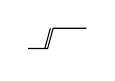
\begin{tikzpicture}[baseline=-0.4ex,x=1em,y=1ex]\draw (0,0)--(0.7,0)--(0.9,1.7)--(2.1,1.7);\draw (0.6,0)--(0.8,1.7);\end{tikzpicture}}}{\par}{author paragraph instruction}{ps_134-4_032-v0018} Of course,  starting with the weakest
kind of homotopy structure on M,  namely just a homotopy relation
$R_h \hand{\in} \mathrm{Hom}_1(M)$,  if $\underline{I}$ is a homotopy interval which is moreover endowed with
\var{\xout{the}}{}{typewriter deletion}{ps_134-4_032-v0019} a structure of a contractor,  \var{\xout{the}}{}{typewriter deletion}{ps_134-4_032-v0020} i.e. \var{\inserted{if $\underline{I}$ is}}{\hand{if $\underline{I}$ is}}{insertion}{ps_134-4_032-v0021} a \var{contradtor}{contractor}{slip corrected}{ps_134-4_032-v0022} such that the
\var{\inserted[typed]{end-point}}{end-point}{typed insertion}{ps_134-4_032-v0023} sections $\hand{\delta}_o\ ,\hand{\delta}_1$  are homotopic,  then I is automatically contractible
(never mind if it is generating or not).  \var{\xout{I get the imp}}{}{typewriter deletion}{ps_134-4_032-v0024}

It seems to me that the homotopy structures I've looked at so far
(such as (Cat) and various standart elementary modelizers $A^{\hand{\wedge}}$) are not only
contractibility structures,  but they \var{\xout{can}}{}{typewriter deletion}{ps_134-4_032-v0025} all can be defined by a single
contractor each.

Besides the \hand{``}\uline{basic} \uline{contractor}\hand{''} $\hand{\Delta}_1$ in (Cat),  there are two general ways
I've met so far for getting contractors.  $\overset{\hand{\unsure{\scriptscriptstyle\perp\perp}}}{\underset{\hand{\unsure{\scriptscriptstyle,\frown}}}{\text{\var{\over[typed]{\illegible{1}}{O}}{O}{typewriter overwriting}{ps_134-4_032-v0026}ne}}}$ \var{\xout{is}}{}{typewriter deletion}{ps_134-4_032-v0027} has been made explicit in
these notes a number of times,  namely the \uline{Lawvere element} \var{\xout{in}}{}{typewriter deletion}{ps_134-4_032-v0028} $L_M$  in M

\margin{32}

%% END SOURCE ps_134-4_032
\ifnum\EditionMode=1
\psapparatusstart
\psentry{ps_134-4_032-v0001}{1}{typed insertion}{\inserted[typed]{an}}{an}{The typed insertion is incorporated at its indicated position; insertion brackets leave the running text.}
\psentry{ps_134-4_032-v0002}{2}{typewriter deletion}{\xout{with}}{}{The typewriter strikes out this material; it leaves the corrected running text.}
\psentry{ps_134-4_032-v0003}{3}{deletion}{\deleted{at least when M is stable under products,}}{}{The author cancels this material by hand; it leaves the corrected running text.}
\psentry{ps_134-4_032-v0004}{4}{insertion}{\inserted{single}}{\hand{single}}{The handwritten insertion is incorporated at its indicated position; insertion brackets leave the running text.}
\psentry{ps_134-4_032-v0005}{5}{typewriter deletion}{\xout{element in}}{}{The typewriter strikes out this material; it leaves the corrected running text.}
\psentry{ps_134-4_032-v0006}{6}{typewriter deletion}{\xout{structure on}}{}{The typewriter strikes out this material; it leaves the corrected running text.}
\psentry{ps_134-4_032-v0007}{7}{typewriter deletion}{\xout{\unsure{I satisfies th}}}{}{The typewriter strikes out this material; it leaves the corrected running text.}
\psentry{ps_134-4_032-v0008}{8}{typed insertion}{\inserted[typed]{map}}{map}{The typed insertion is incorporated at its indicated position; insertion brackets leave the running text.}
\psentry{ps_134-4_032-v0009}{9}{typewriter deletion}{\xout{functor}}{}{The typewriter strikes out this material; it leaves the corrected running text.}
\psentry{ps_134-4_032-v0010}{10}{typed insertion}{\inserted[typed]{tied by a}}{tied by a}{The typed insertion is incorporated at its indicated position; insertion brackets leave the running text.}
\psentry{ps_134-4_032-v0011}{11}{typewriter deletion}{\xout{\illegible{1}}}{}{The typewriter strikes out this material; it leaves the corrected running text.}
\psentry{ps_134-4_032-v0012}{12}{insertion}{\inserted{or by a $\check{\underline{I}}$-homotopy.}}{\hand{or by a $\check{\underline{I}}$-homotopy.}}{The handwritten insertion is incorporated at its indicated position; insertion brackets leave the running text.}
\psentry{ps_134-4_032-v0013}{13}{typewriter deletion}{\xout{\illegible{1}}}{}{The typewriter strikes out this material; it leaves the corrected running text.}
\psentry{ps_134-4_032-v0014}{14}{deletion}{\deleted{n}}{}{The author cancels this material by hand; it leaves the corrected running text.}
\psentry{ps_134-4_032-v0015}{15}{writing over}{\over{\unsure{interactor}}{contractor}}{\hand{contractor}}{The superposed handwritten reading replaces the underlying reading.}
\psentry{ps_134-4_032-v0016}{16}{deletion}{\deleted{n}}{}{The author cancels this material by hand; it leaves the corrected running text.}
\psentry{ps_134-4_032-v0017}{17}{writing over}{\over{\unsure{interactor}}{contractor}}{\hand{contractor}}{The superposed handwritten reading replaces the underlying reading.}
\psentry{ps_134-4_032-v0018}{18}{author paragraph instruction}{\diagram{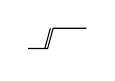
\begin{tikzpicture}[baseline=-0.4ex,x=1em,y=1ex]\draw (0,0)--(0.7,0)--(0.9,1.7)--(2.1,1.7);\draw (0.6,0)--(0.8,1.7);\end{tikzpicture}}}{\par}{The doubled stepped mark instructs a paragraph before Of course.}
\psentry{ps_134-4_032-v0019}{19}{typewriter deletion}{\xout{the}}{}{The typewriter strikes out this material; it leaves the corrected running text.}
\psentry{ps_134-4_032-v0020}{20}{typewriter deletion}{\xout{the}}{}{The typewriter strikes out this material; it leaves the corrected running text.}
\psentry{ps_134-4_032-v0021}{21}{insertion}{\inserted{if $\underline{I}$ is}}{\hand{if $\underline{I}$ is}}{The handwritten insertion is incorporated at its indicated position; insertion brackets leave the running text.}
\psentry{ps_134-4_032-v0022}{22}{slip corrected}{contradtor}{contractor}{Isolated d for c, settled by correctly typed contractor on the same page.}
\psentry{ps_134-4_032-v0023}{23}{typed insertion}{\inserted[typed]{end-point}}{end-point}{The typed insertion is incorporated at its indicated position; insertion brackets leave the running text.}
\psentry{ps_134-4_032-v0024}{24}{typewriter deletion}{\xout{I get the imp}}{}{The typewriter strikes out this material; it leaves the corrected running text.}
\psentry{ps_134-4_032-v0025}{25}{typewriter deletion}{\xout{can}}{}{The typewriter strikes out this material; it leaves the corrected running text.}
\psentry{ps_134-4_032-v0026}{26}{typewriter overwriting}{\over[typed]{\illegible{1}}{O}}{O}{The superposed typed reading replaces the underlying reading.}
\psentry{ps_134-4_032-v0027}{27}{typewriter deletion}{\xout{is}}{}{The typewriter strikes out this material; it leaves the corrected running text.}
\psentry{ps_134-4_032-v0028}{28}{typewriter deletion}{\xout{in}}{}{The typewriter strikes out this material; it leaves the corrected running text.}
\psapparatusend
\fi
\pssource{ps_134-4_033}{134-4/33}{https://grothendieck.umontpellier.fr/web/viewer.html?file=../134-4.pdf\#page=34}
\psnumber{ps_134-4_033-v0001}{1}
\psnumber{ps_134-4_033-v0002}{2}
\psnumber{ps_134-4_033-v0003}{3}
\psnumber{ps_134-4_033-v0004}{4}
\psnumber{ps_134-4_033-v0005}{5}
\psnumber{ps_134-4_033-v0006}{6}
\psnumber{ps_134-4_033-v0007}{7}
\psnumber{ps_134-4_033-v0008}{8}
\psnumber{ps_134-4_033-v0009}{9}
\psnumber{ps_134-4_033-v0010}{10}
\psnumber{ps_134-4_033-v0011}{11}
\psnumber{ps_134-4_033-v0012}{12}
\psnumber{ps_134-4_033-v0013}{13}
\psnumber{ps_134-4_033-v0014}{14}
\psnumber{ps_134-4_033-v0015}{15}
\psnumber{ps_134-4_033-v0016}{16}
\psnumber{ps_134-4_033-v0017}{17}
\psnumber{ps_134-4_033-v0018}{18}
\psnumber{ps_134-4_033-v0019}{19}
\psnumber{ps_134-4_033-v0020}{20}
\psnumber{ps_134-4_033-v0021}{21}
\psnumber{ps_134-4_033-v0022}{22}
%% BEGIN SOURCE ps_134-4_033
% Pursuing Stacks (cotes 134-2 to 134-8): archive cote 134-4, site page 33 (PDF page 34), typescript page 121.
% typescript. Draft compared: ps3.tex:1628-1694.
% AI-transcribed by Claude Opus 5.5 (claude-opus-5-5, adaptive thinking, effort high), Message Batches API, batch ps2 (msgbatch_01NVwr1Yuo8qJf5rykeGBXPK), 2026-11-12; image review recorded in records/CHECK_DECISIONS_134_3_4.tsv.
\scanpage{134-4/33}
\mspage{121}
if it exists,  and if moreover M has a \uline{strict} initia\var{\over[typed]{h}{l}}{l}{typewriter overwriting}{ps_134-4_033-v0001} element, $\hand{\varnothing}_{M}$ .  Re-%
call that $L_{M}$  represents the contravariant functor on M
\[ X \hand{\ensuremath{\longmapsto}} \text{ set of all subobjects of } X \text{ ,} \]
and that the``full'' and ``empty'' subobjects of X,  for variable X,  define
two sections $\hand{\ensuremath{\delta}}_{o}$ and $\hand{\ensuremath{\delta}}_{1}$ of $L_{M}$ .  \var{\over[typed]{E}{I}}{I}{typewriter overwriting}{ps_134-4_033-v0002} forgot to state the extra condition that
% NOTE: the right edge of the scan cuts off the ends of several lines (here "tha[t]")
in M fibered products exist (intersection of two subobjects would be
\var{\xout{associative (commutative)}}{}{typewriter deletion}{ps_134-4_033-v0003}
enough);  then the intersection law endows $L_{M}$ with a structure of a contra\unsure{c}%
% NOTE: line cut off at the right edge after "contra"
tor \var{\inserted[typed]{$\underline{L}_{M}$}}{$\underline{L}_{M}$}{typed insertion}{ps_134-4_033-v0004}, admitting $\hand{\ensuremath{\delta}}_{o}$ as a unit and $\hand{\ensuremath{\delta}}_{1}$ as a zero element.  Moreover,  it is
clear that $L_{M}$ as an interval is separated,  i.e\hand{,} Ker$(\hand{\ensuremath{\delta}}_{o},\hand{\ensuremath{\delta}}_{1}) = \hand{\varnothing}_{M}$ .  M\unsure{\var{\over{e}{o}}{\hand{o}}{writing over}{ps_134-4_033-v0005}}re
precisely still,  $L_{M}$ can be viewed as a \uline{final object} \var{\over[typed]{in}{of}}{of}{typewriter overwriting}{ps_134-4_033-v0006} \uline{the  category}
\uline{of all} \uline{separated} \uline{intervals in} M,  namely for any such interval,  there is
a \uline{unique} map of intervals
\[ \underline{I} \hand{\ensuremath{\longrightarrow}} L_{M} \text{ .} \]
This implies that if M is endowed with a homotopy structure,  such that
there exists a weak homotopy interval which is separated,  then $\underline{L}_{M}$ is such
an interval,  and it is moreover contractible.\var{\deleted{\xout{and}}}{}{deletion}{ps_134-4_033-v0007}  It is doubtful though,
even if we can find a \var{\deleted{\xout{separ}}}{}{deletion}{ps_134-4_033-v0008} \uline{generating} contractor for the given homotopy
structure on M,  that the Law\unsure{\var{\over{e}{e}}{\hand{e}}{writing over}{ps_134-4_033-v0009}}vere contractor is generating too.

Here now is a second interesting way of getting contractors.  We
assume that M admits finite products (as usual).  Let X be an object,  and
assume the object \uline{Hom}(X,X),  representing the functor
\[ Y \hand{\ensuremath{\longmapsto}} \mathrm{Hom}(X\mathrm{x}Y,X) \ = \ \mathrm{Hom}_{Y}(X_{Y},X_{Y}) \text{ ,} \]
exists in M.  (NB  $X_{Y}$  denotes XxY, viewed as an object of $M_{/Y}$.)\hand{.}  Composi%
% NOTE: line cut off at the right edge after "Composi"
-tion of endomorphisms of $X_{Y}$ clearly endow this functor with an \var{\inserted[typed]{associative}}{associative}{typed insertion}{ps_134-4_033-v0010} composition
\var{las,}{law,}{slip corrected}{ps_134-4_033-v0011}  admitting a two-sided unit, which I call $\hand{\ensuremath{e}}_{o}$ .  \var{\xout{(NB}}{}{typewriter deletion}{ps_134-4_033-v0012} Notice that
sections of \var{\xout{\unsure{Hom $\underline{I}=$}}}{}{typewriter deletion}{ps_134-4_033-v0013}
\[ \underline{I} = \underline{\mathrm{Hom}}(X,X) \]
can be identified with maps X \hand{$\rightarrow$} X,  and the section corresponding to id$_{X}$
is of course the two-sided unit.  On the other hand,  if X admits sections
% NOTE: line cut off at the right edge after "sections"
i.e. admits ``constant'' endomorphisms,  it is clear that the corresponding
sections of \underline{I} are \var{\xout{right}}{}{typewriter deletion}{ps_134-4_033-v0014} left zero elements.  If we choose \var{\xout{such}}{}{typewriter deletion}{ps_134-4_033-v0015} a section\var{\xout{\unsure{,}}}{}{typewriter deletion}{ps_134-4_033-v0016}
of X,  \underline{I}  becomes a contractor.  It's interest lies in the following

\uline{Proposition}  Assume \var{\xout{xx}}{}{typewriter deletion}{ps_134-4_033-v0017} finite products exist in M,  and M endowed with
a homotopy structure  \var{\deleted{of type Hom\hand{$_{3}$}  (a weak homotopy interval structure)}}{of type Hom\hand{$_{3}$}  (a weak homotopy interval structure)}{author stet restoration}{ps_134-4_033-v0018}.
\margin{\diagram{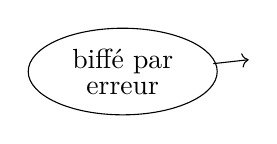
\begin{tikzpicture}[x=1cm,y=1cm,baseline]\draw (0,0) ellipse (1.2 and 0.55);\node at (0,0) {\shortstack{biffé par\\erreur}};\draw[->] (1.15,0.1)--(1.6,0.15);\end{tikzpicture}}} Let X be an object of M endowed with a section $o_{X}$ ,  and suppose \var{\over[typed]{t}{T}}{T}{typewriter overwriting}{ps_134-4_033-v0019}he
object \uline{Hom}(X,X) exists,  hence a contractor \underline{I} as seen above.  The follo\unsure{\var{\over{w}{w}}{\hand{w}}{writing over}{ps_134-4_033-v0020}}-%
wing \var{\inserted{two}}{\hand{two}}{insertion}{ps_134-4_033-v0021} conditions are equivalent:

a)  X is contractible

b)  \underline{I} is contractible (or,  equivalently as seen above\hand{,} \underline{I} is a we\var{\over{a}{a}}{\hand{a}}{writing over}{ps_134-4_033-v0022}k
homotopy interval, namely the two endpoints are homotopic).

\margin{33}

%% END SOURCE ps_134-4_033
\ifnum\EditionMode=1
\psapparatusstart
\psentry{ps_134-4_033-v0001}{1}{typewriter overwriting}{\over[typed]{h}{l}}{l}{The superposed typed reading replaces the underlying reading.}
\psentry{ps_134-4_033-v0002}{2}{typewriter overwriting}{\over[typed]{E}{I}}{I}{The superposed typed reading replaces the underlying reading.}
\psentry{ps_134-4_033-v0003}{3}{typewriter deletion}{\xout{associative (commutative)}}{}{The typewriter strikes out this material; it leaves the corrected running text.}
\psentry{ps_134-4_033-v0004}{4}{typed insertion}{\inserted[typed]{$\underline{L}_{M}$}}{$\underline{L}_{M}$}{The typed insertion is incorporated at its indicated position; insertion brackets leave the running text.}
\psentry{ps_134-4_033-v0005}{5}{writing over}{\over{e}{o}}{\hand{o}}{The superposed handwritten reading replaces the underlying reading.}
\psentry{ps_134-4_033-v0006}{6}{typewriter overwriting}{\over[typed]{in}{of}}{of}{The superposed typed reading replaces the underlying reading.}
\psentry{ps_134-4_033-v0007}{7}{deletion}{\deleted{\xout{and}}}{}{The author cancels this material by hand; it leaves the corrected running text.}
\psentry{ps_134-4_033-v0008}{8}{deletion}{\deleted{\xout{separ}}}{}{The author cancels this material by hand; it leaves the corrected running text.}
\psentry{ps_134-4_033-v0009}{9}{writing over}{\over{e}{e}}{\hand{e}}{The superposed handwritten reading replaces the underlying reading.}
\psentry{ps_134-4_033-v0010}{10}{typed insertion}{\inserted[typed]{associative}}{associative}{The typed insertion is incorporated at its indicated position; insertion brackets leave the running text.}
\psentry{ps_134-4_033-v0011}{11}{slip corrected}{las,}{law,}{Isolated s for w, settled by correctly typed law elsewhere in the checked section.}
\psentry{ps_134-4_033-v0012}{12}{typewriter deletion}{\xout{(NB}}{}{The typewriter strikes out this material; it leaves the corrected running text.}
\psentry{ps_134-4_033-v0013}{13}{typewriter deletion}{\xout{\unsure{Hom $\underline{I}=$}}}{}{The typewriter strikes out this material; it leaves the corrected running text.}
\psentry{ps_134-4_033-v0014}{14}{typewriter deletion}{\xout{right}}{}{The typewriter strikes out this material; it leaves the corrected running text.}
\psentry{ps_134-4_033-v0015}{15}{typewriter deletion}{\xout{such}}{}{The typewriter strikes out this material; it leaves the corrected running text.}
\psentry{ps_134-4_033-v0016}{16}{typewriter deletion}{\xout{\unsure{,}}}{}{The typewriter strikes out this material; it leaves the corrected running text.}
\psentry{ps_134-4_033-v0017}{17}{typewriter deletion}{\xout{xx}}{}{The typewriter strikes out this material; it leaves the corrected running text.}
\psentry{ps_134-4_033-v0018}{18}{author stet restoration}{\deleted{of type Hom\hand{$_{3}$}  (a weak homotopy interval structure)}}{of type Hom\hand{$_{3}$}  (a weak homotopy interval structure)}{The author marks the deletion as biffé par erreur and restores it with dashed stet marks.}
\psentry{ps_134-4_033-v0019}{19}{typewriter overwriting}{\over[typed]{t}{T}}{T}{The superposed typed reading replaces the underlying reading.}
\psentry{ps_134-4_033-v0020}{20}{writing over}{\over{w}{w}}{\hand{w}}{The superposed handwritten reading replaces the underlying reading.}
\psentry{ps_134-4_033-v0021}{21}{insertion}{\inserted{two}}{\hand{two}}{The handwritten insertion is incorporated at its indicated position; insertion brackets leave the running text.}
\psentry{ps_134-4_033-v0022}{22}{writing over}{\over{a}{a}}{\hand{a}}{The superposed handwritten reading replaces the underlying reading.}
\psapparatusend
\fi
\pssource{ps_134-4_034}{134-4/34}{https://grothendieck.umontpellier.fr/web/viewer.html?file=../134-4.pdf\#page=35}
\psnumber{ps_134-4_034-v0001}{1}
\psnumber{ps_134-4_034-v0002}{2}
\psnumber{ps_134-4_034-v0003}{3}
\psnumber{ps_134-4_034-v0004}{4}
\psnumber{ps_134-4_034-v0005}{5}
\psnumber{ps_134-4_034-v0006}{6}
\psnumber{ps_134-4_034-v0007}{7}
\psnumber{ps_134-4_034-v0008}{8}
\psnumber{ps_134-4_034-v0009}{9}
\psnumber{ps_134-4_034-v0010}{10}
\psnumber{ps_134-4_034-v0011}{11}
\psnumber{ps_134-4_034-v0012}{12}
\psnumber{ps_134-4_034-v0013}{13}
\psnumber{ps_134-4_034-v0014}{14}
\psnumber{ps_134-4_034-v0015}{15}
\psnumber{ps_134-4_034-v0016}{16}
\psnumber{ps_134-4_034-v0017}{17}
\psnumber{ps_134-4_034-v0018}{18}
\psnumber{ps_134-4_034-v0019}{19}
\psnumber{ps_134-4_034-v0020}{20}
\psnumber{ps_134-4_034-v0021}{21}
\psnumber{ps_134-4_034-v0022}{22}
\psnumber{ps_134-4_034-v0023}{23}
%% BEGIN SOURCE ps_134-4_034
% Pursuing Stacks (cotes 134-2 to 134-8): archive cote 134-4, site page 34 (PDF page 35), typescript page 122.
% typescript. Draft compared: ps3.tex:1677-1752.
% AI-transcribed by Claude Opus 5.5 (claude-opus-5-5, adaptive thinking, effort high), Message Batches API, batch ps2 (msgbatch_01NVwr1Yuo8qJf5rykeGBXPK), 2026-11-12; image review recorded in records/CHECK_DECISIONS_134_3_4.tsv.
\scanpage{134-4/34}
\mspage{122}
Moreover, \var{\xout{if}}{}{typewriter deletion}{ps_134-4_034-v0001} this condition \var{\xout{\unsure{is satisfied, we}}}{}{typewriter deletion}{ps_134-4_034-v0002}\var{\inserted[typed]{implies the}}{implies the}{typed insertion}{ps_134-4_034-v0003} following two:

c)\quad For any object Y in M, if \underline{Hom}(Y,X) exists, it is contractible.

d)\quad F$\overset{\hand{\smile}}{\underset{\hand{\frown}}{\mathrm o}}$r any Y in M, if Hom(X,Y) exists, the natural map
\[ Y \hand{\to} \underline{Hom}(X,Y) \]
(identifying Y to the ``subobject of constant maps from X to Y'') is a
homotopism.

T\var{\over[typed]{h}{h}}{h}{typewriter overwriting}{ps_134-4_034-v0004}e equivalence of a) and b) is just a tautological translation
of \var{\xout{the homotopy}}{}{typewriter deletion}{ps_134-4_034-v0005}\var{\inserted[typed]{contractibility}}{contractibility}{typed insertion}{ps_134-4_034-v0006} \var{\inserted{and homotopy relation}}{\hand{and homotopy relation}}{insertion}{ps_134-4_034-v0007} in terms of \var{\deleted{elementary}}{}{deletion}{ps_134-4_034-v0008} weak homotopy intervals $\underline{J}$ \var{\inserted{(cf. cor. 2 below)}}{\hand{(cf. cor. 2 below)}}{insertion}{ps_134-4_034-v0009}.
T\var{\over{H}{h}}{\hand{h}}{writing over}{ps_134-4_034-v0010}at c\hand{)} and d\hand{)} follow comes from the fact that the monoïd\var{\xout{\illegible{1}}}{}{typewriter deletion}{ps_134-4_034-v0011} object
$I = \underline{End}(X,X) = \underline{Hom}(X,X)$ operates on the left on \underline{Hom}(Y,X), on the right
on \underline{Hom}(X,Y), and the following :

\uline{Corollary}\hand{1}. Let $\underline{I}$ be a \var{\xout{contractible contractor}}{}{typewriter deletion}{ps_134-4_034-v0012}\var{\inserted[typed]{weak homotopy interval}}{weak homotopy interval}{typed insertion}{ps_134-4_034-v0013}, assume the underlying I
``operates'' on an object H , namely we are given a map
\[ h: I\mathrm{x}H \hand{\longrightarrow} H \qquad (\text{``operation'' of I on H}) \]
satisfying the relations (where h(u,f) is written simply u.f ):
\[ \var{\xout{xx}}{}{typewriter deletion}{ps_134-4_034-v0014}\ e_o.f = f \quad , \quad e_1\hand{(}e_1\var{\over{\illegible{1}}{\cdot}}{\hand{\cdot}}{writing over}{ps_134-4_034-v0015}f) = e_1.\ f \quad , \]
namely $e_o$ acts as the identity, and $\hand{e_1}$ acts as an idempotent \var{\inserted[typed]{p on H}}{p on H}{typed insertion}{ps_134-4_034-v0016} (a very
weak associativity assumption indeed \var{\inserted[typed]{if I is a contractor}}{if I is a contractor}{typed insertion}{ps_134-4_034-v0017}, as $e_1\hand{\circ}e_1 = e_1$). Assume the image
of p i.e. Ker($id_H$,p) exists, let $H_o$ be the corresponding subobject of
H, and \var{\deleted{p}}{}{deletion}{ps_134-4_034-v0018}
\[ p_o : H \hand{\longrightarrow} H_o \]
the map induced by p. T$\overset{\hand{\scriptscriptstyle\perp\perp}}{\underset{\hand{\scriptscriptstyle,\frown}}{\mathrm h}}$en $p_o$ is a homotopism (and hence the inclusion
\var{\inserted[typed]{i:}}{i:}{typed insertion}{ps_134-4_034-v0019}$H_o \hand{\longrightarrow} H$, which is a section of $p_o$ , is a homotopism too).

Because of the saturation \var{\xout{condition}}{}{typewriter deletion}{ps_134-4_034-v0020}\var{\inserted[typed]{property c')}}{property c')}{typed insertion}{ps_134-4_034-v0021} of homotopies, it is enough to
check that $p = ip_o$ is a homotopism (as $pi_o = id_{H_o}$ already is one), and
for this it is enough to see it is homotopic to the identity map of H.
But a homotopy between the two is realized by h, \var{\deleted{\unsure{hence}}}{}{deletion}{ps_134-4_034-v0022} qed.

T$\overset{\hand{\scriptscriptstyle\perp\perp}}{\underset{\hand{\scriptscriptstyle,\frown}}{\mathrm h}}$e argument for equivalence of a) and b) above can be generalized
as follows:

\uline{Corollary} 2 . Let M be as before, and X and Y objects such that
$H = \underline{Hom}(X,Y)$ exists in M. Let $f,g: X \hand{\rightrightarrows} Y$ be two maps, which we'll
identify to the corresponding sections of H. Then f and g are homotopic
maps iff they gi\var{\over{\illegible{1}}{v}}{\hand{v}}{writing over}{ps_134-4_034-v0023}e rise to homotopic sections of H.

F)\quad \uline{T$\overset{\hand{\scriptscriptstyle\perp\perp}}{\underset{\hand{\scriptscriptstyle,\frown}}{\mathrm h}}$e canonical homotopy structure} : \hand{\uline{preliminaries on} $\pi_o$ .}

In order to simplify life, I will in this section make the follo-%
wing assumptions on M (which presumably, except for the first, could be

\margin{34}

%% END SOURCE ps_134-4_034
\ifnum\EditionMode=1
\psapparatusstart
\psentry{ps_134-4_034-v0001}{1}{typewriter deletion}{\xout{if}}{}{The typewriter strikes out this material; it leaves the corrected running text.}
\psentry{ps_134-4_034-v0002}{2}{typewriter deletion}{\xout{\unsure{is satisfied, we}}}{}{The typewriter strikes out this material; it leaves the corrected running text.}
\psentry{ps_134-4_034-v0003}{3}{typed insertion}{\inserted[typed]{implies the}}{implies the}{The typed insertion is incorporated at its indicated position; insertion brackets leave the running text.}
\psentry{ps_134-4_034-v0004}{4}{typewriter overwriting}{\over[typed]{h}{h}}{h}{The superposed typed reading replaces the underlying reading.}
\psentry{ps_134-4_034-v0005}{5}{typewriter deletion}{\xout{the homotopy}}{}{The typewriter strikes out this material; it leaves the corrected running text.}
\psentry{ps_134-4_034-v0006}{6}{typed insertion}{\inserted[typed]{contractibility}}{contractibility}{The typed insertion is incorporated at its indicated position; insertion brackets leave the running text.}
\psentry{ps_134-4_034-v0007}{7}{insertion}{\inserted{and homotopy relation}}{\hand{and homotopy relation}}{The handwritten insertion is incorporated at its indicated position; insertion brackets leave the running text.}
\psentry{ps_134-4_034-v0008}{8}{deletion}{\deleted{elementary}}{}{The author cancels this material by hand; it leaves the corrected running text.}
\psentry{ps_134-4_034-v0009}{9}{insertion}{\inserted{(cf. cor. 2 below)}}{\hand{(cf. cor. 2 below)}}{The handwritten insertion is incorporated at its indicated position; insertion brackets leave the running text.}
\psentry{ps_134-4_034-v0010}{10}{writing over}{\over{H}{h}}{\hand{h}}{The superposed handwritten reading replaces the underlying reading.}
\psentry{ps_134-4_034-v0011}{11}{typewriter deletion}{\xout{\illegible{1}}}{}{The typewriter strikes out this material; it leaves the corrected running text.}
\psentry{ps_134-4_034-v0012}{12}{typewriter deletion}{\xout{contractible contractor}}{}{The typewriter strikes out this material; it leaves the corrected running text.}
\psentry{ps_134-4_034-v0013}{13}{typed insertion}{\inserted[typed]{weak homotopy interval}}{weak homotopy interval}{The typed insertion is incorporated at its indicated position; insertion brackets leave the running text.}
\psentry{ps_134-4_034-v0014}{14}{typewriter deletion}{$\xout{xx}$}{}{The typewriter strikes out this material; it leaves the corrected running text.}
\psentry{ps_134-4_034-v0015}{15}{writing over}{$\over{\illegible{1}}{\cdot}$}{$\hand{\cdot}$}{The superposed handwritten reading replaces the underlying reading.}
\psentry{ps_134-4_034-v0016}{16}{typed insertion}{\inserted[typed]{p on H}}{p on H}{The typed insertion is incorporated at its indicated position; insertion brackets leave the running text.}
\psentry{ps_134-4_034-v0017}{17}{typed insertion}{\inserted[typed]{if I is a contractor}}{if I is a contractor}{The typed insertion is incorporated at its indicated position; insertion brackets leave the running text.}
\psentry{ps_134-4_034-v0018}{18}{deletion}{\deleted{p}}{}{The author cancels this material by hand; it leaves the corrected running text.}
\psentry{ps_134-4_034-v0019}{19}{typed insertion}{\inserted[typed]{i:}}{i:}{The typed insertion is incorporated at its indicated position; insertion brackets leave the running text.}
\psentry{ps_134-4_034-v0020}{20}{typewriter deletion}{\xout{condition}}{}{The typewriter strikes out this material; it leaves the corrected running text.}
\psentry{ps_134-4_034-v0021}{21}{typed insertion}{\inserted[typed]{property c')}}{property c')}{The typed insertion is incorporated at its indicated position; insertion brackets leave the running text.}
\psentry{ps_134-4_034-v0022}{22}{deletion}{\deleted{\unsure{hence}}}{}{The author cancels this material by hand; it leaves the corrected running text.}
\psentry{ps_134-4_034-v0023}{23}{writing over}{\over{\illegible{1}}{v}}{\hand{v}}{The superposed handwritten reading replaces the underlying reading.}
\psapparatusend
\fi
\pssource{ps_134-4_035}{134-4/35}{https://grothendieck.umontpellier.fr/web/viewer.html?file=../134-4.pdf\#page=36}
\psnumber{ps_134-4_035-v0001}{1}
\psnumber{ps_134-4_035-v0002}{2}
\psnumber{ps_134-4_035-v0003}{3}
\psnumber{ps_134-4_035-v0004}{4}
\psnumber{ps_134-4_035-v0005}{5}
\psnumber{ps_134-4_035-v0006}{6}
\psnumber{ps_134-4_035-v0007}{7}
\psnumber{ps_134-4_035-v0008}{8}
\psnumber{ps_134-4_035-v0009}{9}
\psnumber{ps_134-4_035-v0010}{10}
\psnumber{ps_134-4_035-v0011}{11}
\psnumber{ps_134-4_035-v0012}{12}
\psnumber{ps_134-4_035-v0013}{13}
\psnumber{ps_134-4_035-v0014}{14}
\psnumber{ps_134-4_035-v0015}{15}
\psnumber{ps_134-4_035-v0016}{16}
\psnumber{ps_134-4_035-v0017}{17}
\psnumber{ps_134-4_035-v0018}{18}
\psnumber{ps_134-4_035-v0019}{19}
\psnumber{ps_134-4_035-v0020}{20}
\psnumber{ps_134-4_035-v0021}{21}
\psnumber{ps_134-4_035-v0022}{22}
\psnumber{ps_134-4_035-v0023}{23}
\psnumber{ps_134-4_035-v0024}{24}
%% BEGIN SOURCE ps_134-4_035
% Pursuing Stacks (cotes 134-2 to 134-8): archive cote 134-4, site page 35 (PDF page 36), typescript page 123.
% typescript. Draft compared: ps3.tex:1734-1810.
% AI-transcribed by Claude Opus 5.5 (claude-opus-5-5, adaptive thinking, effort high), Message Batches API, batch ps2 (msgbatch_01NVwr1Yuo8qJf5rykeGBXPK), 2026-11-12; image review recorded in records/CHECK_DECISIONS_134_3_4.tsv.
\scanpage{134-4/35}
\mspage{\hand{123}}
considerably weakened,  but these will be sufficient):

a)  Finite products exist in M\hand{. (``pour mémoire'').}

b)  Arbitrary sums exist in M,  they are ``disjoint'' and ``universal''
(which implies that M has a \uline{strict} initial o\var{\over{\unsure{b}}{b}}{\hand{b}}{writing over}{ps_134-4_035-v0001}\var{\over{j}{j}}{\hand{j}}{writing over}{ps_134-4_035-v0002}ect).

c)  E\var{\over[typed]{v}{v}}{v}{typewriter overwriting}{ps_134-4_035-v0003}ery object in M is isomorphic to a direct sum of O-connected one\hand{s.}

I recall an object is called \uline{O-connected} if it is  a)``non empty'' i.e.
non isomorphic to $\emptyset_M$ ,  and b) connected,  i.e. any decomposition of it
into a sum of two \var{\inserted[typed]{sub}}{sub}{typed insertion}{ps_134-4_035-v0004}objects  is trivial (namely, one is ``empty'',  the other
is ``full''). Also,  under the assumption b),  well known standart argu-%
ments show that for any object \var{\inserted[typed]{X}}{X}{typed insertion}{ps_134-4_035-v0005}, a decomposition of X into a direct sum
of \var{\over{O}{\unsure{\O}}}{\hand{\unsure{\O}}}{writing over}{ps_134-4_035-v0006}-connected subobjects is essentially \var{uniqqe}{unique}{slip corrected}{ps_134-4_035-v0007} (namely the \var{\inserted[typed]{corresponding}}{corresponding}{typed insertion}{ps_134-4_035-v0008} set of subob-%
jects of X \var{\inserted{is unique}}{\hand{is unique}}{insertion}{ps_134-4_035-v0009}), if it exists\var{\over{,}{.}}{\hand{.}}{writing over}{ps_134-4_035-v0010} \var{\deleted{is necessarily unique.}}{}{deletion}{ps_134-4_035-v0011} T$\overset{\hand{\scriptscriptstyle\perp\perp}}{\underset{\hand{\scriptscriptstyle,\frown}}{\mathrm h}}$e  subobjects \var{\deleted{that}}{}{deletion}{ps_134-4_035-v0012}
occuring in the sum are called the \uline{connected components} of X ,  and the
set of connected components of X is denoted as usual by $\hand{\pi}_o$(X).  We thus
get a natural functor
\[ X \hand{\mapsto} \var{\xout{\illegible{1}(X)}}{}{typewriter deletion}{ps_134-4_035-v0013}\,\hand{\pi}_o(X) \quad , \qquad M \hand{\to} (Sets) \quad \hand{.} \]
\var{\xout{Which}}{}{typewriter deletion}{ps_134-4_035-v0014}\var{\inserted[typed]{This}}{This}{typed insertion}{ps_134-4_035-v0015} can be equally described as a \uline{left} \uline{adjoint} to the functor
\[ E \hand{\longmapsto} E_M \quad , \qquad (Sets) \hand{\longrightarrow} M \quad , \]
associating to a set E the corresponding ``\uline{constant} \uline{object}'' E$_M$ of M,  some-%
times also denoted by the product symbol Exe$_M$ = Exe  (e the final object
of M ),  namely the direct sum \var{\inserted[typed]{in \over{M}{M}}}{in \hand{M}}{typed insertion}{ps_134-4_035-v0016} of E copies of e.  The adjunction formula
is
\[ \mathrm{Hom}_M(X,E_M) \hand{\simeq} \mathrm{Hom}_{(Sets)}(\hand{\pi}_o(X),E\ ) \quad . \]
The adjunction \var{\xout{formula}}{}{typewriter deletion}{ps_134-4_035-v0017} relation implies that  the functor $\hand{\pi}_o$  commutes
with \var{\inserted[typed]{all}}{all}{typed insertion}{ps_134-4_035-v0018} direct limits  which exist in M,  and in particular (and trivially so)
to direct sums.

I'll finally assume also,  to fix the ideas :

d)  T\var{\over[typed]{H}{h}}{h}{typewriter overwriting}{ps_134-4_035-v0019}e final object of M is O-connected i.e. $\hand{\pi}_o$(e) = one point set.

Empty objects of M,\var{\xout{xxx}}{}{typewriter deletion}{ps_134-4_035-v0020} on the other hand,  are of course characterized
by the condition
\[ \hand{\pi}_o(\emptyset_M) = \emptyset \quad . \]

Finally,  I'll make in the end a very strong assumption on M , which
ho\var{\over{wever}{wever}}{\hand{wever}}{writing over}{ps_134-4_035-v0021} is satisfied more or less trivially in the cases we are interested
in,  when M is a would-be modelizer:

e)  (Total O-asphericity of M):  the product of tw\var{\over[typed]{p}{o}}{o}{typewriter overwriting}{ps_134-4_035-v0022} O-connected ob-%
ject\var{\over{s}{s}}{\hand{s}}{writing over}{ps_134-4_035-v0023} of M is again O-connected.

This is clearly equiv\var{\over{\unsure{alen}}{alen}}{\hand{alen}}{writing over}{ps_134-4_035-v0024}t to the condition

e')  T$\overset{\hand{\scriptscriptstyle\perp\perp}}{\underset{\hand{\scriptscriptstyle,\frown}}{\mathrm h}}$e functor $\hand{\pi}_o$ : M $\hand{\to}$(Sets)  commutes to finite products.

\margin{35}

%% END SOURCE ps_134-4_035
\ifnum\EditionMode=1
\psapparatusstart
\psentry{ps_134-4_035-v0001}{1}{writing over}{\over{\unsure{b}}{b}}{\hand{b}}{The superposed handwritten reading replaces the underlying reading.}
\psentry{ps_134-4_035-v0002}{2}{writing over}{\over{j}{j}}{\hand{j}}{The superposed handwritten reading replaces the underlying reading.}
\psentry{ps_134-4_035-v0003}{3}{typewriter overwriting}{\over[typed]{v}{v}}{v}{The superposed typed reading replaces the underlying reading.}
\psentry{ps_134-4_035-v0004}{4}{typed insertion}{\inserted[typed]{sub}}{sub}{The typed insertion is incorporated at its indicated position; insertion brackets leave the running text.}
\psentry{ps_134-4_035-v0005}{5}{typed insertion}{\inserted[typed]{X}}{X}{The typed insertion is incorporated at its indicated position; insertion brackets leave the running text.}
\psentry{ps_134-4_035-v0006}{6}{writing over}{\over{O}{\unsure{\O}}}{\hand{\unsure{\O}}}{The superposed handwritten reading replaces the underlying reading.}
\psentry{ps_134-4_035-v0007}{7}{slip corrected}{uniqqe}{unique}{Isolated q for u, with unique correctly typed later on the same page and elsewhere in the checked section.}
\psentry{ps_134-4_035-v0008}{8}{typed insertion}{\inserted[typed]{corresponding}}{corresponding}{The typed insertion is incorporated at its indicated position; insertion brackets leave the running text.}
\psentry{ps_134-4_035-v0009}{9}{insertion}{\inserted{is unique}}{\hand{is unique}}{The handwritten insertion is incorporated at its indicated position; insertion brackets leave the running text.}
\psentry{ps_134-4_035-v0010}{10}{writing over}{\over{,}{.}}{\hand{.}}{The superposed handwritten reading replaces the underlying reading.}
\psentry{ps_134-4_035-v0011}{11}{deletion}{\deleted{is necessarily unique.}}{}{The author cancels this material by hand; it leaves the corrected running text.}
\psentry{ps_134-4_035-v0012}{12}{deletion}{\deleted{that}}{}{The author cancels this material by hand; it leaves the corrected running text.}
\psentry{ps_134-4_035-v0013}{13}{typewriter deletion}{$\xout{\illegible{1}(X)}$}{}{The typewriter strikes out this material; it leaves the corrected running text.}
\psentry{ps_134-4_035-v0014}{14}{typewriter deletion}{\xout{Which}}{}{The typewriter strikes out this material; it leaves the corrected running text.}
\psentry{ps_134-4_035-v0015}{15}{typed insertion}{\inserted[typed]{This}}{This}{The typed insertion is incorporated at its indicated position; insertion brackets leave the running text.}
\psentry{ps_134-4_035-v0016}{16}{typed insertion}{\inserted[typed]{in \over{M}{M}}}{in \hand{M}}{The typed insertion is incorporated at its indicated position; insertion brackets leave the running text.}
\psentry{ps_134-4_035-v0017}{17}{typewriter deletion}{\xout{formula}}{}{The typewriter strikes out this material; it leaves the corrected running text.}
\psentry{ps_134-4_035-v0018}{18}{typed insertion}{\inserted[typed]{all}}{all}{The typed insertion is incorporated at its indicated position; insertion brackets leave the running text.}
\psentry{ps_134-4_035-v0019}{19}{typewriter overwriting}{\over[typed]{H}{h}}{h}{The superposed typed reading replaces the underlying reading.}
\psentry{ps_134-4_035-v0020}{20}{typewriter deletion}{\xout{xxx}}{}{The typewriter strikes out this material; it leaves the corrected running text.}
\psentry{ps_134-4_035-v0021}{21}{writing over}{\over{wever}{wever}}{\hand{wever}}{The superposed handwritten reading replaces the underlying reading.}
\psentry{ps_134-4_035-v0022}{22}{typewriter overwriting}{\over[typed]{p}{o}}{o}{The superposed typed reading replaces the underlying reading.}
\psentry{ps_134-4_035-v0023}{23}{writing over}{\over{s}{s}}{\hand{s}}{The superposed handwritten reading replaces the underlying reading.}
\psentry{ps_134-4_035-v0024}{24}{writing over}{\over{\unsure{alen}}{alen}}{\hand{alen}}{The superposed handwritten reading replaces the underlying reading.}
\psapparatusend
\fi
\pssource{ps_134-4_036}{134-4/36}{https://grothendieck.umontpellier.fr/web/viewer.html?file=../134-4.pdf\#page=37}
\psnumber{ps_134-4_036-v0001}{1}
\psnumber{ps_134-4_036-v0002}{2}
\psnumber{ps_134-4_036-v0003}{3}
\psnumber{ps_134-4_036-v0004}{4}
\psnumber{ps_134-4_036-v0005}{5}
\psnumber{ps_134-4_036-v0006}{6}
\psnumber{ps_134-4_036-v0007}{7}
\psnumber{ps_134-4_036-v0008}{8}
\psnumber{ps_134-4_036-v0009}{9}
\psnumber{ps_134-4_036-v0010}{10}
\psnumber{ps_134-4_036-v0011}{11}
\psnumber{ps_134-4_036-v0012}{12}
\psnumber{ps_134-4_036-v0013}{13}
\psnumber{ps_134-4_036-v0014}{14}
\psnumber{ps_134-4_036-v0015}{15}
\psnumber{ps_134-4_036-v0016}{16}
\psnumber{ps_134-4_036-v0017}{17}
\psnumber{ps_134-4_036-v0018}{18}
\psnumber{ps_134-4_036-v0019}{19}
\psnumber{ps_134-4_036-v0020}{20}
\psnumber{ps_134-4_036-v0021}{21}
\psnumber{ps_134-4_036-v0022}{22}
\psnumber{ps_134-4_036-v0023}{23}
\psnumber{ps_134-4_036-v0024}{24}
%% BEGIN SOURCE ps_134-4_036
% Pursuing Stacks (cotes 134-2 to 134-8): archive cote 134-4, site page 36 (PDF page 37), typescript page 124.
% typescript. Draft compared: ps3.tex:1792-1856.
% AI-transcribed by Claude Opus 5.5 (claude-opus-5-5, adaptive thinking, effort high), Message Batches API, batch ps2 (msgbatch_01NVwr1Yuo8qJf5rykeGBXPK), 2026-11-12; image review recorded in records/CHECK_DECISIONS_134_3_4.tsv.
\scanpage{134-4/36}
\mspage{124}

\uline{Remark s}. The crucial assumptions here seem to be b) (which allows \var{\deleted{to \xout{\unsure{defin}}}}{}{deletion}{ps_134-4_036-v0001}\var{\inserted{definition}}{\hand{definition}}{insertion}{ps_134-4_036-v0002}
\var{\deleted{define}}{}{deletion}{ps_134-4_036-v0003}\var{\inserted{of}}{\hand{of}}{insertion}{ps_134-4_036-v0004} a $\hand{\pi}_0$ functor, and topological intuition tied up with connectedness
to enter into play\hand{)}, and e), which implies that \var{\over{wi}{wi}}{\hand{wi}}{writing over}{ps_134-4_036-v0005}th respect to cartesi-%
an products, the usual intuitive background for connectedness, rooted in
the example of M = (topological spaces), is indeed valid. This condition
is clearly stronger than d), which is a mere condition for convenience
in itself (otherwise, a decomposition of e into connected components
would mean a corresponding decomposition of M \var{\over{a}{a}}{\hand{a}}{writing over}{ps_134-4_036-v0006}\var{\over{\unsure{s}}{s}}{\hand{s}}{writing over}{ps_134-4_036-v0007} a product \var{\inserted{category}}{\hand{category}}{insertion}{ps_134-4_036-v0008}, and every -%
thing could be looked at ``componentwise''\hand{)}. As for c), it could probably
be dispensed with, by \var{\xout{interpreting}}{}{typewriter deletion}{ps_134-4_036-v0009}\var{\inserted[typed]{still defining}}{still defining}{typed insertion}{ps_134-4_036-v0010} $\hand{\pi}_0$(X) as a strict pro-set. In the
case of modelizers anyhow, such generalization seems quite besides the
point.

The condition e), however innocent-looking in terms of topological
intuition, seems to me an extremely strong condition indeed. I suspect
that in case M is a topos, it is equivalent to total asphericity. In any
case, if M is the topos associated to a \var{\inserted[typed]{locally connected}}{locally connected}{typed insertion}{ps_134-4_036-v0011} topological space, we've seen
time ago \var{\xout{this is}}{}{typewriter deletion}{ps_134-4_036-v0012} that \var{\xout{the}}{}{typewriter deletion}{ps_134-4_036-v0013} the condition \var{\xout{implies}}{}{typewriter deletion}{ps_134-4_036-v0014} e) implies X is irredu-%
cible, and hence totally aspheric. In view of this exactingness of e),
I'll not use it unless specifically stated.

\hand{3.4.}

\hand{52.} Before pursuing the review of ``pure homotopy notions'' begun in yes-%
terday's notes, I would like first to correct some inaccuracies which
\var{\over{\illegible{1}}{flew}}{\hand{flew}}{writing over}{ps_134-4_036-v0015} in when l\var{\over{o}{o}}{\hand{o}}{writing over}{ps_134-4_036-v0016}oking at the relationship between the two first basic
homotopy notions, namely the notion of a homotopy relation, and the \var{\xout{xxx}}{}{typewriter deletion}{ps_134-4_036-v0017}
notion of a homotopism structure. \var{\inserted{As usual,}}{\hand{As usual,}}{insertion}{ps_134-4_036-v0018} \var{\deleted{The inaccuracies were caused by the}}{}{deletion}{ps_134-4_036-v0019}
\var{\deleted{fact that while starting on the notes,}}{}{deletion}{ps_134-4_036-v0020}\var{\inserted{\deleted{came from}}}{\hand{}}{insertion}{ps_134-4_036-v0021} \hand{the} provisional image I had in mind
\var{\deleted{being}}{}{deletion}{ps_134-4_036-v0022}\var{\inserted{was}}{\hand{was}}{insertion}{ps_134-4_036-v0023} still somewhat vague, \hand{while} the reasonable expectations came out more
clearly through the process of writing things down (including factual in-%
accuracies \hand{!}).

The two notions clearly correspond to two kind of ways of construc-%
ting new categories M' in terms of a given one, and a functor
\[ M \hand{\longrightarrow} M' \]
which is bijective o\var{\over{\unsure{f}}{n}}{\hand{n}}{writing over}{ps_134-4_036-v0024} objects, and has the property moreover that for
any category C, the corresponding functor
\[ \underline{Hom}(M',C) \hand{\longrightarrow} \underline{Hom}(M,C) \]
is a fully faithful embedding in the strict sense, namely injective on

\margin{36}

%% END SOURCE ps_134-4_036
\ifnum\EditionMode=1
\psapparatusstart
\psentry{ps_134-4_036-v0001}{1}{deletion}{\deleted{to \xout{\unsure{defin}}}}{}{The author cancels this material by hand; it leaves the corrected running text.}
\psentry{ps_134-4_036-v0002}{2}{insertion}{\inserted{definition}}{\hand{definition}}{The handwritten insertion is incorporated at its indicated position; insertion brackets leave the running text.}
\psentry{ps_134-4_036-v0003}{3}{deletion}{\deleted{define}}{}{The author cancels this material by hand; it leaves the corrected running text.}
\psentry{ps_134-4_036-v0004}{4}{insertion}{\inserted{of}}{\hand{of}}{The handwritten insertion is incorporated at its indicated position; insertion brackets leave the running text.}
\psentry{ps_134-4_036-v0005}{5}{writing over}{\over{wi}{wi}}{\hand{wi}}{The superposed handwritten reading replaces the underlying reading.}
\psentry{ps_134-4_036-v0006}{6}{writing over}{\over{a}{a}}{\hand{a}}{The superposed handwritten reading replaces the underlying reading.}
\psentry{ps_134-4_036-v0007}{7}{writing over}{\over{\unsure{s}}{s}}{\hand{s}}{The superposed handwritten reading replaces the underlying reading.}
\psentry{ps_134-4_036-v0008}{8}{insertion}{\inserted{category}}{\hand{category}}{The handwritten insertion is incorporated at its indicated position; insertion brackets leave the running text.}
\psentry{ps_134-4_036-v0009}{9}{typewriter deletion}{\xout{interpreting}}{}{The typewriter strikes out this material; it leaves the corrected running text.}
\psentry{ps_134-4_036-v0010}{10}{typed insertion}{\inserted[typed]{still defining}}{still defining}{The typed insertion is incorporated at its indicated position; insertion brackets leave the running text.}
\psentry{ps_134-4_036-v0011}{11}{typed insertion}{\inserted[typed]{locally connected}}{locally connected}{The typed insertion is incorporated at its indicated position; insertion brackets leave the running text.}
\psentry{ps_134-4_036-v0012}{12}{typewriter deletion}{\xout{this is}}{}{The typewriter strikes out this material; it leaves the corrected running text.}
\psentry{ps_134-4_036-v0013}{13}{typewriter deletion}{\xout{the}}{}{The typewriter strikes out this material; it leaves the corrected running text.}
\psentry{ps_134-4_036-v0014}{14}{typewriter deletion}{\xout{implies}}{}{The typewriter strikes out this material; it leaves the corrected running text.}
\psentry{ps_134-4_036-v0015}{15}{writing over}{\over{\illegible{1}}{flew}}{\hand{flew}}{The superposed handwritten reading replaces the underlying reading.}
\psentry{ps_134-4_036-v0016}{16}{writing over}{\over{o}{o}}{\hand{o}}{The superposed handwritten reading replaces the underlying reading.}
\psentry{ps_134-4_036-v0017}{17}{typewriter deletion}{\xout{xxx}}{}{The typewriter strikes out this material; it leaves the corrected running text.}
\psentry{ps_134-4_036-v0018}{18}{insertion}{\inserted{As usual,}}{\hand{As usual,}}{The handwritten insertion is incorporated at its indicated position; insertion brackets leave the running text.}
\psentry{ps_134-4_036-v0019}{19}{deletion}{\deleted{The inaccuracies were caused by the}}{}{The author cancels this material by hand; it leaves the corrected running text.}
\psentry{ps_134-4_036-v0020}{20}{deletion}{\deleted{fact that while starting on the notes,}}{}{The author cancels this material by hand; it leaves the corrected running text.}
\psentry{ps_134-4_036-v0021}{21}{insertion}{\inserted{\deleted{came from}}}{\hand{}}{The handwritten insertion is incorporated at its indicated position; insertion brackets leave the running text.}
\psentry{ps_134-4_036-v0022}{22}{deletion}{\deleted{being}}{}{The author cancels this material by hand; it leaves the corrected running text.}
\psentry{ps_134-4_036-v0023}{23}{insertion}{\inserted{was}}{\hand{was}}{The handwritten insertion is incorporated at its indicated position; insertion brackets leave the running text.}
\psentry{ps_134-4_036-v0024}{24}{writing over}{\over{\unsure{f}}{n}}{\hand{n}}{The superposed handwritten reading replaces the underlying reading.}
\psapparatusend
\fi
\pssource{ps_134-4_037}{134-4/37}{https://grothendieck.umontpellier.fr/web/viewer.html?file=../134-4.pdf\#page=38}
\psnumber{ps_134-4_037-v0001}{1}
\psnumber{ps_134-4_037-v0002}{2}
\psnumber{ps_134-4_037-v0003}{3}
\psnumber{ps_134-4_037-v0004}{4}
\psnumber{ps_134-4_037-v0005}{5}
\psnumber{ps_134-4_037-v0006}{6}
\psnumber{ps_134-4_037-v0007}{7}
\psnumber{ps_134-4_037-v0008}{8}
\psnumber{ps_134-4_037-v0009}{9}
\psnumber{ps_134-4_037-v0010}{10}
\psnumber{ps_134-4_037-v0011}{11}
\psnumber{ps_134-4_037-v0012}{12}
%% BEGIN SOURCE ps_134-4_037
% Pursuing Stacks (cotes 134-2 to 134-8): archive cote 134-4, site page 37 (PDF page 38), typescript page 125.
% typescript. Draft compared: ps3.tex:1841-1908.
% AI-transcribed by Claude Opus 5.5 (claude-opus-5-5, adaptive thinking, effort high), Message Batches API, batch ps2 (msgbatch_01NVwr1Yuo8qJf5rykeGBXPK), 2026-11-12; image review recorded in records/CHECK_DECISIONS_134_3_4.tsv.
\scanpage{134-4/37}
\mspage{125}
objects. O$\overset{\hand{\scriptscriptstyle\perp\perp}}{\mathrm n}$e way is to take for $M'$ any quotient category of $M$, by an
equivalence relation which is the discrete one on objects - thus $M'$ cor-%
responds just to an equivalence relation $R$ in $F\hand{\ell}(M)$, compatible with
\var{\xout{compositi}}{}{typewriter deletion}{ps_134-4_037-v0001} the source and target maps and with compositions. T$\overset{\hand{\scriptscriptstyle\perp\perp}}{\underset{\hand{\scriptscriptstyle,\frown}}{\mathrm h}}$e other is
to take as $M'$ a localization with respect to some $W\hand{\subset}F\hand{\ell}(M)$, and if we
take $W$ strongly saturated we get a bijective correspondance between those
$M'$ and the \var{\xout{corresponding}}{}{typewriter deletion}{ps_134-4_037-v0002} set of strongly saturated subsets $W$ of $F\hand{\ell}(M)$.

It would'nt be any more reasonable to call an arbitrary $R$ as above,
corresponding to an arbitrary quotient category $M'$ with same objects as
$M$, a ``homotopy relation'' o\var{\over{\unsure{f}}{n}}{\hand{n}}{writing over}{ps_134-4_037-v0003} $M$ (as I did though yesterday), as it would
be to call an arbitrary strongly saturated $W\hand{\subset}F\hand{\ell}(M)$ a ``homotopism struc-%
ture'' on $M$ (as I nearly did yesterday, but then rectified in the stride)\hand{.}
\uline{T$\overset{\hand{\scriptscriptstyle\perp\perp}}{\underset{\hand{\scriptscriptstyle,\frown}}{\mathrm h}}$e characteristic flavor of homotopy theory comes in}, \uline{when we got an}
$M'$ \uline{which is} \uline{both} \uline{a quotient category and a localization of} $M$. Thus \var{\xout{neithe}}{}{typewriter deletion}{ps_134-4_037-v0004}
neither approach, via $R$ or via $W$, is any more contained in the other\hand{,}
than \var{\xout{to}}{}{typewriter deletion}{ps_134-4_037-v0005} the converse. \var{\over{W}{W}}{\hand{W}}{writing over}{ps_134-4_037-v0006}e should regard the \uline{homotopy structure} on $M$ to
be embodied in the basic functor
\[ M \hand{\longrightarrow} M' \quad , \]
which is a description where no choice yet is made between the two possib-%
le descriptions of $M'$, either by an $R$, or by a $W$. If we describe $M'$ in
terms of $R$, the extra assumption to make on $R$ for calling it a ``\uline{homotopy}
\uline{relation}'', is \var{\xout{the\illegible{1}}}{}{typewriter deletion}{ps_134-4_037-v0007} that the \var{\inserted[typed]{canonical}}{canonical}{typed insertion}{ps_134-4_037-v0008} functor
\[ M \hand{\longrightarrow} M/R \]
should be localizing. Alternatively, describing $M'$ by $W$, the extra
assumption to make on $W$ (as we did yesterday) in order to call $W$ a \uline{homoto-}%
\uline{pism} \uline{structure} on $M$, is that the canonical \var{\inserted[typed]{localization}}{localization}{typed insertion}{ps_134-4_037-v0009} functor
\[ M \hand{\longrightarrow} W^{-1}M \]
be essentially a passage-to-quotient functor, namely \var{\inserted[typed]{sur}}{sur}{typed insertion}{ps_134-4_037-v0010}\var{\xout{bi}}{}{typewriter deletion}{ps_134-4_037-v0011}jective on arrows
(as we know already it is bijective on objects). Thus the set of all
homotopy relations on $M$ is in one to one correspondance with the set of
all homotopism structures on $M$, and if we denote these sets (in accordan-%
ce with yesterday's provisional notations) $\mathrm{Hom}_1(M)$ and $\mathrm{Hom}_2(M)$, we get
thus a \uline{bijective} correspondance
\[ \mathrm{Hom}_1(M) \hand{\longleftrightarrow} \mathrm{Hom}_2(M) \qquad . \]
T$\overset{\hand{\scriptscriptstyle\perp\perp}}{\underset{\hand{\scriptscriptstyle,\frown}}{\mathrm h}}$e set of homotopy structures $\mathrm{Hom}(M)$ on $M$ may be either defined as the
usual quotient set defined by the previous two-member system of transitive
bijections between sets, or more substantially, as a set of isomorphism
classes of \unsure{\diagram{\begin{tikzpicture}[baseline=(q.base)]\node[inner sep=0pt] (q) {``};\draw[color=blue,line width=.6pt] (q.west) ++(.015,.02) -- ++(-.02,.11) -- ++(.04,.09) -- ++(.02,.06);\end{tikzpicture}}}categories $M'$ ``under $M$'' i.e. endowed with a functor $M\hand{\to} M'$\,$\overset{\hand{-}}{,}$
\var{\inserted{and}}{\hand{and}}{insertion}{ps_134-4_037-v0012} subject to the following two extra conditions:

\margin{37}

%% END SOURCE ps_134-4_037
\ifnum\EditionMode=1
\psapparatusstart
\psentry{ps_134-4_037-v0001}{1}{typewriter deletion}{\xout{compositi}}{}{The typewriter strikes out this material; it leaves the corrected running text.}
\psentry{ps_134-4_037-v0002}{2}{typewriter deletion}{\xout{corresponding}}{}{The typewriter strikes out this material; it leaves the corrected running text.}
\psentry{ps_134-4_037-v0003}{3}{writing over}{\over{\unsure{f}}{n}}{\hand{n}}{The superposed handwritten reading replaces the underlying reading.}
\psentry{ps_134-4_037-v0004}{4}{typewriter deletion}{\xout{neithe}}{}{The typewriter strikes out this material; it leaves the corrected running text.}
\psentry{ps_134-4_037-v0005}{5}{typewriter deletion}{\xout{to}}{}{The typewriter strikes out this material; it leaves the corrected running text.}
\psentry{ps_134-4_037-v0006}{6}{writing over}{\over{W}{W}}{\hand{W}}{The superposed handwritten reading replaces the underlying reading.}
\psentry{ps_134-4_037-v0007}{7}{typewriter deletion}{\xout{the\illegible{1}}}{}{The typewriter strikes out this material; it leaves the corrected running text.}
\psentry{ps_134-4_037-v0008}{8}{typed insertion}{\inserted[typed]{canonical}}{canonical}{The typed insertion is incorporated at its indicated position; insertion brackets leave the running text.}
\psentry{ps_134-4_037-v0009}{9}{typed insertion}{\inserted[typed]{localization}}{localization}{The typed insertion is incorporated at its indicated position; insertion brackets leave the running text.}
\psentry{ps_134-4_037-v0010}{10}{typed insertion}{\inserted[typed]{sur}}{sur}{The typed insertion is incorporated at its indicated position; insertion brackets leave the running text.}
\psentry{ps_134-4_037-v0011}{11}{typewriter deletion}{\xout{bi}}{}{The typewriter strikes out this material; it leaves the corrected running text.}
\psentry{ps_134-4_037-v0012}{12}{insertion}{\inserted{and}}{\hand{and}}{The handwritten insertion is incorporated at its indicated position; insertion brackets leave the running text.}
\psapparatusend
\fi
\pssource{ps_134-4_038}{134-4/38}{https://grothendieck.umontpellier.fr/web/viewer.html?file=../134-4.pdf\#page=39}
\psnumber{ps_134-4_038-v0001}{1}
\psnumber{ps_134-4_038-v0002}{2}
\psnumber{ps_134-4_038-v0003}{3}
\psnumber{ps_134-4_038-v0004}{4}
\psnumber{ps_134-4_038-v0005}{5}
\psnumber{ps_134-4_038-v0006}{6}
\psnumber{ps_134-4_038-v0007}{7}
\psnumber{ps_134-4_038-v0008}{8}
\psnumber{ps_134-4_038-v0009}{9}
\psnumber{ps_134-4_038-v0010}{10}
\psnumber{ps_134-4_038-v0011}{11}
\psnumber{ps_134-4_038-v0012}{12}
\psnumber{ps_134-4_038-v0013}{13}
\psnumber{ps_134-4_038-v0014}{14}
\psnumber{ps_134-4_038-v0015}{15}
\psnumber{ps_134-4_038-v0016}{16}
\psnumber{ps_134-4_038-v0017}{17}
\psnumber{ps_134-4_038-v0018}{18}
\psnumber{ps_134-4_038-v0019}{19}
\psnumber{ps_134-4_038-v0020}{20}
\psnumber{ps_134-4_038-v0021}{21}
\psnumber{ps_134-4_038-v0022}{22}
\psnumber{ps_134-4_038-v0023}{23}
\psnumber{ps_134-4_038-v0024}{24}
\psnumber{ps_134-4_038-v0025}{25}
\psnumber{ps_134-4_038-v0026}{26}
\psnumber{ps_134-4_038-v0027}{27}
\psnumber{ps_134-4_038-v0028}{28}
%% BEGIN SOURCE ps_134-4_038
% Pursuing Stacks (cotes 134-2 to 134-8): archive cote 134-4, site page 38 (PDF page 39), typescript page 126.
% typescript. Draft compared: ps3.tex:1891-1967.
% AI-transcribed by Claude Opus 5.5 (claude-opus-5-5, adaptive thinking, effort high), Message Batches API, batch ps2 (msgbatch_01NVwr1Yuo8qJf5rykeGBXPK), 2026-11-12; image review recorded in records/CHECK_DECISIONS_134_3_4.tsv.
\scanpage{134-4/38}
\mspage{126}
a)\quad T\var{\over{H}{h}}{\hand{h}}{writing over}{ps_134-4_038-v0001}e functor M\hand{$\to$}M' is bijective on objects,  surjective on arrows.
b)\quad The functor M\hand{$\to$}M' is a localization functor \hand{(}i\var{\over{t}{t}}{\hand{t}}{writing over}{ps_134-4_038-v0002} w\var{\over{ill}{ill}}{\hand{ill}}{writing over}{ps_134-4_038-v0003} be so then,  in
view of a),  in the strict sense,  namely M' will be \var{\inserted[typed]{M-}}{M-}{typed insertion}{ps_134-4_038-v0004}isomorphic,  no\hand{t}
only \var{\inserted[typed]{M-}}{M-}{typed insertion}{ps_134-4_038-v0005}equivalent, to a localization $W^{-1}M$ ).

However,  the question arises w\var{\over{\unsure{h}}{h}}{\hand{h}}{writing over}{ps_134-4_038-v0006}\var{\over{e}{e}}{\hand{e}}{writing over}{ps_134-4_038-v0007}ther it is possible to define \var{\over{s}{s}}{\hand{s}}{writing over}{ps_134-4_038-v0008}uch
a homotopy structure on M,  in terms of an arbitrary R i.e. an arbitrary
quotient category having same objects  (let Q(M)=Q the set of all such R's)\hand{,}
or in terms of an arbitrary localization of M,  or what amounts to the sam
% NOTE: the right edge of the scan cuts the ends of some lines (``sam'', ``definin'', ``relatio'', ``clear'', ``injectiv'')
me,  in terms of an arbitrary strongly saturated W\hand{$\subset$}$F\var{\over{l}{\ell}}{\hand{\ell}}{writing over}{ps_134-4_038-v0009}$(M)  (let's call
L(M)=L  the set of all such W's).  T$\overset{\hand{\scriptscriptstyle\perp\perp}}{\underset{\hand{\scriptscriptstyle,\frown}}{\mathrm h}}$e first thing that comes to mind
here,  is that we got two natural maps
% Hand-drawn arrows are marked blue; typed objects remain plain.
\hand{(1)} \diagram{\begin{tikzcd} Q \arrow[r, bend left, "r", color=blue] \& L \arrow[l, bend left, "s", color=blue] \end{tikzcd}}
between Q and L,  which are defined by the observation that whenever we
have a functor \var{\inserted{i:}}{\hand{i:}}{insertion}{ps_134-4_038-v0010} M\hand{$\to$}M' , \var{\inserted[typed]{injective on ob\over{j}{j}ects\hand{,}}}{injective on ob\hand{j}ects\hand{,}}{typed insertion}{ps_134-4_038-v0011} it defines both an R\hand{$\in$}Q  (namely f\hand{$\sim$}$_{R}$g  iff
i(f)=i(g))  and a W\hand{$\in$}L (namely f\hand{$\in$}W  iff u(f) is invertible).  \var{\over{\unsure{f}}{F}}{\hand{F}}{writing over}{ps_134-4_038-v0012}or defining
r(R)  resp. s(\var{\over{\unsure{W}}{W}}{\hand{W}}{writing over}{ps_134-4_038-v0013}),  we apply this to the case when M' = M/R  resp. $W^{-1}$M.
Let's look a little at the two cases separately.

Start with R \var{\inserted[typed]{in Q}}{in Q}{typed insertion}{ps_134-4_038-v0014}, we get W=r(R),
\[ W = \hand{\{} f \hand{\in} F\var{\over{l}{\ell}}{\hand{\ell}}{writing over}{ps_134-4_038-v0015}(M) \hand{\mid} i(f) \text{ invertible}\hand{\}} \hand{,} \]
where
\[ i:\ M \hand{\to} M/R \]
is the canonical functor;  we thus get a canonical functor (compatible
with the structures ``under M'' )
\[ (\var{\over{*}{2}}{\hand{2}}{writing over}{ps_134-4_038-v0016}) \qquad \var{\deleted{\xout{\illegible{1}}}}{}{deletion}{ps_134-4_038-v0017}\hand{\ensuremath{\alpha=\alpha_{R}}}:\ M_W \hand{\to} M_R \hand{,} \]
where for simplicity I write
\[ M_R = M/R \ ,\ \ M_W = W^{-1}M \ . \]
We may define W as the largest element in L (for the natural order relatio\unsure{n}
in L namely inclusion of subsets of $F\var{\over{l}{\ell}}{\hand{\ell}}{writing over}{ps_134-4_038-v0018}$(M))  such that a functor (*)
exists (compatible with the functors from M into both sides)  -  such a
functor of course is unique (by the preliminaries on functors M\hand{$\to$}M' made
at the beginning).  \var{\xout{Now}}{}{typewriter deletion}{ps_134-4_038-v0019} In terms of (\var{\over{\unsure{*}}{2}}{\hand{2}}{writing over}{ps_134-4_038-v0020}),  we can say that R is \var{\inserted{actually}}{\hand{actually}}{insertion}{ps_134-4_038-v0021} a homotopy
relation  (let's call $Q_o$(M)=$Q_o$ the \var{\xout{corresponding}}{}{typewriter deletion}{ps_134-4_038-v0022} subset of Q\var{\deleted{\unsure{'s}}}{}{deletion}{ps_134-4_038-v0023} of all such
\var{\xout{Now start with}}{}{typewriter deletion}{ps_134-4_038-v0024}
relations)  iff \var{\deleted{(*}}{}{deletion}{ps_134-4_038-v0025} (\hand{2}) is an isomorphism, or equivalently (as it is clear
ly bijective on \var{\xout{arrows}}{}{typewriter deletion}{ps_134-4_038-v0026} objects,  surjective on arrows)  if\hand{f} it is \uline{injectiv\hand{e}
on arrows}\hand{,} i.e. \uline{faithful}.

Conversely,  start now with W in L ,  we get R=s(W) ,
\[ R = \hand{\{}(f,g)\hand{\in} F\var{\over{l}{\ell}}{\hand{\ell}}{writing over}{ps_134-4_038-v0027}(M)\mathrm{x}F\var{\over{l}{\ell}}{\hand{\ell}}{writing over}{ps_134-4_038-v0028}(M) \hand{\mid} i(f)=i(g)\hand{\}} \ , \]
\margin{38}

%% END SOURCE ps_134-4_038
\ifnum\EditionMode=1
\psapparatusstart
\psentry{ps_134-4_038-v0001}{1}{writing over}{\over{H}{h}}{\hand{h}}{The superposed handwritten reading replaces the underlying reading.}
\psentry{ps_134-4_038-v0002}{2}{writing over}{\over{t}{t}}{\hand{t}}{The superposed handwritten reading replaces the underlying reading.}
\psentry{ps_134-4_038-v0003}{3}{writing over}{\over{ill}{ill}}{\hand{ill}}{The superposed handwritten reading replaces the underlying reading.}
\psentry{ps_134-4_038-v0004}{4}{typed insertion}{\inserted[typed]{M-}}{M-}{The typed insertion is incorporated at its indicated position; insertion brackets leave the running text.}
\psentry{ps_134-4_038-v0005}{5}{typed insertion}{\inserted[typed]{M-}}{M-}{The typed insertion is incorporated at its indicated position; insertion brackets leave the running text.}
\psentry{ps_134-4_038-v0006}{6}{writing over}{\over{\unsure{h}}{h}}{\hand{h}}{The superposed handwritten reading replaces the underlying reading.}
\psentry{ps_134-4_038-v0007}{7}{writing over}{\over{e}{e}}{\hand{e}}{The superposed handwritten reading replaces the underlying reading.}
\psentry{ps_134-4_038-v0008}{8}{writing over}{\over{s}{s}}{\hand{s}}{The superposed handwritten reading replaces the underlying reading.}
\psentry{ps_134-4_038-v0009}{9}{writing over}{$\over{l}{\ell}$}{$\hand{\ell}$}{The superposed handwritten reading replaces the underlying reading.}
\psentry{ps_134-4_038-v0010}{10}{insertion}{\inserted{i:}}{\hand{i:}}{The handwritten insertion is incorporated at its indicated position; insertion brackets leave the running text.}
\psentry{ps_134-4_038-v0011}{11}{typed insertion}{\inserted[typed]{injective on ob\over{j}{j}ects\hand{,}}}{injective on ob\hand{j}ects\hand{,}}{The typed insertion is incorporated at its indicated position; insertion brackets leave the running text.}
\psentry{ps_134-4_038-v0012}{12}{writing over}{\over{\unsure{f}}{F}}{\hand{F}}{The superposed handwritten reading replaces the underlying reading.}
\psentry{ps_134-4_038-v0013}{13}{writing over}{\over{\unsure{W}}{W}}{\hand{W}}{The superposed handwritten reading replaces the underlying reading.}
\psentry{ps_134-4_038-v0014}{14}{typed insertion}{\inserted[typed]{in Q}}{in Q}{The typed insertion is incorporated at its indicated position; insertion brackets leave the running text.}
\psentry{ps_134-4_038-v0015}{15}{writing over}{$\over{l}{\ell}$}{$\hand{\ell}$}{The superposed handwritten reading replaces the underlying reading.}
\psentry{ps_134-4_038-v0016}{16}{writing over}{$\over{*}{2}$}{$\hand{2}$}{The superposed handwritten reading replaces the underlying reading.}
\psentry{ps_134-4_038-v0017}{17}{deletion}{$\deleted{\xout{\illegible{1}}}$}{}{The author cancels this material by hand; it leaves the corrected running text.}
\psentry{ps_134-4_038-v0018}{18}{writing over}{$\over{l}{\ell}$}{$\hand{\ell}$}{The superposed handwritten reading replaces the underlying reading.}
\psentry{ps_134-4_038-v0019}{19}{typewriter deletion}{\xout{Now}}{}{The typewriter strikes out this material; it leaves the corrected running text.}
\psentry{ps_134-4_038-v0020}{20}{writing over}{\over{\unsure{*}}{2}}{\hand{2}}{The superposed handwritten reading replaces the underlying reading.}
\psentry{ps_134-4_038-v0021}{21}{insertion}{\inserted{actually}}{\hand{actually}}{The handwritten insertion is incorporated at its indicated position; insertion brackets leave the running text.}
\psentry{ps_134-4_038-v0022}{22}{typewriter deletion}{\xout{corresponding}}{}{The typewriter strikes out this material; it leaves the corrected running text.}
\psentry{ps_134-4_038-v0023}{23}{deletion}{\deleted{\unsure{'s}}}{}{The author cancels this material by hand; it leaves the corrected running text.}
\psentry{ps_134-4_038-v0024}{24}{typewriter deletion}{\xout{Now start with}}{}{The typewriter strikes out this material; it leaves the corrected running text.}
\psentry{ps_134-4_038-v0025}{25}{deletion}{\deleted{(*}}{}{The author cancels this material by hand; it leaves the corrected running text.}
\psentry{ps_134-4_038-v0026}{26}{typewriter deletion}{\xout{arrows}}{}{The typewriter strikes out this material; it leaves the corrected running text.}
\psentry{ps_134-4_038-v0027}{27}{writing over}{$\over{l}{\ell}$}{$\hand{\ell}$}{The superposed handwritten reading replaces the underlying reading.}
\psentry{ps_134-4_038-v0028}{28}{writing over}{$\over{l}{\ell}$}{$\hand{\ell}$}{The superposed handwritten reading replaces the underlying reading.}
\psapparatusend
\fi
\pssource{ps_134-4_039}{134-4/39}{https://grothendieck.umontpellier.fr/web/viewer.html?file=../134-4.pdf\#page=40}
\psnumber{ps_134-4_039-v0001}{1}
\psnumber{ps_134-4_039-v0002}{2}
\psnumber{ps_134-4_039-v0003}{3}
\psnumber{ps_134-4_039-v0004}{4}
\psnumber{ps_134-4_039-v0005}{5}
\psnumber{ps_134-4_039-v0006}{6}
\psnumber{ps_134-4_039-v0007}{7}
\psnumber{ps_134-4_039-v0008}{8}
\psnumber{ps_134-4_039-v0009}{9}
\psnumber{ps_134-4_039-v0010}{10}
\psnumber{ps_134-4_039-v0011}{11}
\psnumber{ps_134-4_039-v0012}{12}
\psnumber{ps_134-4_039-v0013}{13}
\psnumber{ps_134-4_039-v0014}{14}
\psnumber{ps_134-4_039-v0015}{15}
\psnumber{ps_134-4_039-v0016}{16}
\psnumber{ps_134-4_039-v0017}{17}
\psnumber{ps_134-4_039-v0018}{18}
\psnumber{ps_134-4_039-v0019}{19}
\psnumber{ps_134-4_039-v0020}{20}
%% BEGIN SOURCE ps_134-4_039
% Pursuing Stacks (cotes 134-2 to 134-8): archive cote 134-4, site page 39 (PDF page 40), typescript page 127.
% typescript. Draft compared: ps3.tex:1948-2013.
% AI-transcribed by Claude Opus 5.5 (claude-opus-5-5, adaptive thinking, effort high), Message Batches API, batch ps2 (msgbatch_01NVwr1Yuo8qJf5rykeGBXPK), 2026-11-12; image review recorded in records/CHECK_DECISIONS_134_3_4.tsv.
\scanpage{134-4/39}
\mspage{127}
where now
\[ i\colon M \hand{\to} W^{\hand{-1}}M = M_W \]
is the canonical functor defined in terms of W;  we thus get a canonical \unsure{\var{\over{f}{f}}{\hand{f}}{writing over}{ps_134-4_039-v0001}}
functor of categories ``under M''
\[ (\var{\over{2}{3}}{\hand{3}}{writing over}{ps_134-4_039-v0002}) \qquad \hand{\beta=\beta_W}\colon M_R \hand{\to} M_W \quad , \]
as a matter of fact,  R is the largest element in Q (for the inclusion re-%
lation of subsets of $F\var{\over{l}{\ell}}{\hand{\ell}}{writing over}{ps_134-4_039-v0003}(M)\mathrm{x}F\var{\over{l}{\ell}}{\hand{\ell}}{writing over}{ps_134-4_039-v0004}(M)$) for which a functor (\var{\over{2}{3}}{\hand{3}}{writing over}{ps_134-4_039-v0005}) exists (then ne-%
cessarily unique,  as before).  We may say that W is a homotopism structu-%
re on M,  i.e.  $W\hand{\in}L_0$  (where $L_0$ is the subset of L of all homotopism
structures on M) iff the functor (\var{\over{2}{3}}{\hand{3}}{writing over}{ps_134-4_039-v0006}) is an isomorphism,  or equivalently
(as it is clearly bijective on objects,  \var{\over{\unsure{sur}}{inj}}{\hand{inj}}{writing over}{ps_134-4_039-v0007}ective on arrows)  iff it is
\uline{surjective on arrows} .

We may describe $\var{\over{Q}{Q}}{\hand{Q}}{writing over}{ps_134-4_039-v0008}_0$ and $\var{\over[typed]{L}{L}}{L}{typewriter overwriting}{ps_134-4_039-v0009}_0$ in a purely set theoretic way,  in terms
of the system (r,s) of maps in (1),  by the formula (which is just a
translation of the definitionsof $\var{\over{Q}{Q}}{\hand{Q}}{writing over}{ps_134-4_039-v0010}_0$ and $L_0$)
\[ Q_0 = \hand{\Big\{} q \hand{\in} Q \hand{\big|} sr(q) = q \hand{\Big\}} \]
\[ L_0 = \hand{\Big\{} \ell \hand{\in} L \hand{\big|} rs(\ell) = \ell \hand{\Big\}} \quad , \]

and we can describe formally the pair of subsets $(Q_0,L_0)$  of Q,L  as the
largest pair of subsets, such that r and s induce between $Q_0$ and $L_0$ bijec-%
tions inverse of each other.  In th\var{\over[typed]{\unsure{e}}{i}}{i}{typewriter overwriting}{ps_134-4_039-v0011}s general set-theoretic set up,  it is
by no means clear,  and false in general,  that r maps Q into $L_0$ or L\var{\deleted{$_0$}}{}{deletion}{ps_134-4_039-v0012} int\hand{\unsure{o}}
% NOTE: the line runs off the right edge of the scan after "int"
$Q_{\hand{0}}$ (thus both $Q_0$ and $L_0$ may well be empty,  whereas Q and L are not).  Thu\unsure{s}
it is not clear at all that starting with an arbitrary $R\hand{\in}Q$,  the correspon-%
ding W = r(R)  is a homotopism structure,  and it is easily seen that this
is \uline{not} so in general,\var{\deleted{f}}{}{deletion}{ps_134-4_039-v0013} contrarily to what I hastily stated in yesterday\hand{'}s
notes.  (Take M with just one object,  therefore defined by a monoïd G,
and $M_R$  corresponds to a quotient monoïd \var{\inserted{$G'$}}{\hand{$G'$}}{insertion}{ps_134-4_039-v0014}, we \uline{may} take \var{\over{\unsure{G}}{$G'$}}{\hand{$G'$}}{writing over}{ps_134-4_039-v0015}= unit monoïd,
thus W is G itself, and $M_W$ the enveloping group \var{\inserted{$\overline{G}$}}{\hand{$\overline{G}$}}{insertion}{ps_134-4_039-v0016} of G  -  the \var{\xout{canonical}}{}{typewriter deletion}{ps_134-4_039-v0017} map
$\overline{G} \hand{\to} \var{\over{\unsure{G}}{G'}}{\hand{G'}}{writing over}{ps_134-4_039-v0018}$  need not be \var{\over{\unsure{sur}}{in}}{\hand{in}}{writing over}{ps_134-4_039-v0019}jective ! )\hand{.}In the opposite direction,  starting with
an arbitrary W in L,  the corresponding R need not be a homotopy relation.
(If M is reduced to a point,  this amounts to saying that if we localize
a monoïd G with respect to a subset $W\hand{\subset}G$ ,  by making invertible the ele-%
ment in W,  the corresponding map $G \hand{\to} \overline{G}$ need not be surjective !)

What we may say,  though,  is that if we start with a pair
\[ (R,W) \hand{\in} Q\mathrm{x}L \]
such that the \uline{two} functors (2),(3)  exist,  i.e. such that
\[ W \hand{\leq} r(R) \quad\text{and}\quad R \hand{\leq} s(W) \quad , \]
then \var{\xout{\illegible{1}}}{}{typewriter deletion}{ps_134-4_039-v0020} $(R,W)\hand{\in} Q_0\mathrm{x}L_0$  i.e. R is a homotopy relation and W is a homotopism
\margin{39}

%% END SOURCE ps_134-4_039
\ifnum\EditionMode=1
\psapparatusstart
\psentry{ps_134-4_039-v0001}{1}{writing over}{\over{f}{f}}{\hand{f}}{The superposed handwritten reading replaces the underlying reading.}
\psentry{ps_134-4_039-v0002}{2}{writing over}{$\over{2}{3}$}{$\hand{3}$}{The superposed handwritten reading replaces the underlying reading.}
\psentry{ps_134-4_039-v0003}{3}{writing over}{$\over{l}{\ell}$}{$\hand{\ell}$}{The superposed handwritten reading replaces the underlying reading.}
\psentry{ps_134-4_039-v0004}{4}{writing over}{$\over{l}{\ell}$}{$\hand{\ell}$}{The superposed handwritten reading replaces the underlying reading.}
\psentry{ps_134-4_039-v0005}{5}{writing over}{\over{2}{3}}{\hand{3}}{The superposed handwritten reading replaces the underlying reading.}
\psentry{ps_134-4_039-v0006}{6}{writing over}{\over{2}{3}}{\hand{3}}{The superposed handwritten reading replaces the underlying reading.}
\psentry{ps_134-4_039-v0007}{7}{writing over}{\over{\unsure{sur}}{inj}}{\hand{inj}}{The superposed handwritten reading replaces the underlying reading.}
\psentry{ps_134-4_039-v0008}{8}{writing over}{$\over{Q}{Q}$}{$\hand{Q}$}{The superposed handwritten reading replaces the underlying reading.}
\psentry{ps_134-4_039-v0009}{9}{typewriter overwriting}{$\over[typed]{L}{L}$}{$L$}{The superposed typed reading replaces the underlying reading.}
\psentry{ps_134-4_039-v0010}{10}{writing over}{$\over{Q}{Q}$}{$\hand{Q}$}{The superposed handwritten reading replaces the underlying reading.}
\psentry{ps_134-4_039-v0011}{11}{typewriter overwriting}{\over[typed]{\unsure{e}}{i}}{i}{The superposed typed reading replaces the underlying reading.}
\psentry{ps_134-4_039-v0012}{12}{deletion}{\deleted{$_0$}}{}{The author cancels this material by hand; it leaves the corrected running text.}
\psentry{ps_134-4_039-v0013}{13}{deletion}{\deleted{f}}{}{The author cancels this material by hand; it leaves the corrected running text.}
\psentry{ps_134-4_039-v0014}{14}{insertion}{\inserted{$G'$}}{\hand{$G'$}}{The handwritten insertion is incorporated at its indicated position; insertion brackets leave the running text.}
\psentry{ps_134-4_039-v0015}{15}{writing over}{\over{\unsure{G}}{$G'$}}{\hand{$G'$}}{The superposed handwritten reading replaces the underlying reading.}
\psentry{ps_134-4_039-v0016}{16}{insertion}{\inserted{$\overline{G}$}}{\hand{$\overline{G}$}}{The handwritten insertion is incorporated at its indicated position; insertion brackets leave the running text.}
\psentry{ps_134-4_039-v0017}{17}{typewriter deletion}{\xout{canonical}}{}{The typewriter strikes out this material; it leaves the corrected running text.}
\psentry{ps_134-4_039-v0018}{18}{writing over}{$\over{\unsure{G}}{G'}$}{$\hand{G'}$}{The superposed handwritten reading replaces the underlying reading.}
\psentry{ps_134-4_039-v0019}{19}{writing over}{\over{\unsure{sur}}{in}}{\hand{in}}{The superposed handwritten reading replaces the underlying reading.}
\psentry{ps_134-4_039-v0020}{20}{typewriter deletion}{\xout{\illegible{1}}}{}{The typewriter strikes out this material; it leaves the corrected running text.}
\psapparatusend
\fi
\pssource{ps_134-4_040}{134-4/40}{https://grothendieck.umontpellier.fr/web/viewer.html?file=../134-4.pdf\#page=41}
\psnumber{ps_134-4_040-v0001}{1}
\psnumber{ps_134-4_040-v0002}{2}
\psnumber{ps_134-4_040-v0003}{3}
\psnumber{ps_134-4_040-v0004}{4}
\psnumber{ps_134-4_040-v0005}{5}
\psnumber{ps_134-4_040-v0006}{6}
\psnumber{ps_134-4_040-v0007}{7}
\psnumber{ps_134-4_040-v0008}{8}
\psnumber{ps_134-4_040-v0009}{9}
%% BEGIN SOURCE ps_134-4_040
% Pursuing Stacks (cotes 134-2 to 134-8): archive cote 134-4, site page 40 (PDF page 41), typescript page 128.
% typescript. Draft compared: ps3.tex:1998-2061.
% AI-transcribed by Claude Opus 5.5 (claude-opus-5-5, adaptive thinking, effort high), Message Batches API, batch ps2 (msgbatch_01NVwr1Yuo8qJf5rykeGBXPK), 2026-11-12; image review recorded in records/CHECK_DECISIONS_134_3_4.tsv.
\scanpage{134-4/40}
\mspage{128}

structure, and the two are associated. This comes from the fact that
both compositions of the functors (2),(3) must be the identity functors
(being compatible with the ``under M'' structure), hence \hand{\ensuremath{\alpha}} and \hand{\ensuremath{\beta}} are isomor%
phisms, which shows both R \hand{\ensuremath{\in}} Q$_{\rm o}$ and W \hand{\ensuremath{\in}} L$_{\rm o}$ , and that R and L are associa-%
ted. In terms of the set theoretic situation (1), this may be described
by using the order relations on Q and L, and the fact that r and s are
monotone maps, and satisfy moreover
(*) \qquad $sr(q)\hand{\ensuremath{\leq}} q$ \;,\; $rs(\hand{\ensuremath{\ell}})\hand{\ensuremath{\leq}}\hand{\ensuremath{\ell}}$ \quad (any $q\hand{\ensuremath{\in}}Q$, $\hand{\ensuremath{\ell}}\hand{\ensuremath{\in}}L$) \;,
which implies that the set C$_{\rm o}$ of pairs $(q\unsure{_{,}}\,, \hand{\ensuremath{\ell}})$ of associated elements
of Q$_{\rm o}$,L$_{\rm o}$ can be described also as
\[ C_{o} = \hand{\ensuremath{\{}}(q,\hand{\ensuremath{\ell}})\hand{\ensuremath{\in}} Q\text{x}L \hand{\ensuremath{\mid}} \hand{\ensuremath{\ell}}\hand{\ensuremath{\leq}}r(q),\quad q\hand{\ensuremath{\leq}} s(\hand{\ensuremath{\ell}})) \qquad . \]

Thus it does'nt seem evident to get a homotopy structure on M, just
starting with an\var{\deleted{y}}{}{deletion}{ps_134-4_040-v0001} R \hand{\ensuremath{\in}} Q or \var{\xout{any}}{}{typewriter deletion}{ps_134-4_040-v0002} a W \hand{\ensuremath{\in}} L, without assuming beforehand that
R is a homotopy relation, or W a homotopism structure. T$\overset{\hand{\scriptscriptstyle\perp\perp}}{\underset{\hand{-}}{\mathrm h}}$e condition
$C_{1,2}$ on page 115 may be viewed as a condition on a pair (R,W)\hand{\ensuremath{\in}} QxL,
and it clearly implies
\[ R \hand{\ensuremath{\leq}} s(W) \quad ; \]
if we assume moreover \quad W=r(R) \quad we get \quad R\hand{\ensuremath{\leq}} s(r(R)) \quad and hence, in view
of the first inequality (*) above ,
\[ R = sr(R) \quad \text{i.e.} \quad R \hand{\ensuremath{\in}} Q_{o} \quad , \]
i.e. R is a homotopy relation, as asserted somewhat quickly yesterday.

T$\overset{\hand{\scriptscriptstyle\perp\perp}}{\mathrm h}$e only standart way for getting homotopy structures in a general
category M which I \var{\xout{\illegible{1}}}{}{typewriter deletion}{ps_134-4_040-v0003} can see by now , is in terms of an arbitrary
set \hand{\ensuremath{\Sigma}}$_{h}$ of intervals in M (assuming only that M \var{\over{a}{a}}{\hand{a}}{writing over}{ps_134-4_040-v0004}dmits finite products).
As soon as the focus gets upon intervals for describing homotopy structu-%
res, the situation becomes typically non-autodual - in contrast to
Quillen's autodual treatment of homotopy relations (via``left'' and ``right''
homotopies, involving respectively ``cylinder'' and ``path'' - objects). \var{\xout{Thi}}{}{typewriter deletion}{ps_134-4_040-v0005}
This is in keeping with the \var{\inserted{\unsure{highly|highty} non auto-dual}}{\hand{\unsure{highly|highty} non auto-dual}}{insertion}{ps_134-4_040-v0006} axiom\unsure{\var{\over{s}{s}}{\hand{s}}{writing over}{ps_134-4_040-v0007}} on universal disjoint \var{\uline{sums in M,} which
we finally introduced by the end of yesterday's \uline{reflection.}\diagram{
\begin{tikzpicture}[baseline=-.3ex,x=1em,y=1ex]\draw[color=blue,line width=.5pt] (0,0)--(.12,2.5);\draw[color=blue,line width=.5pt] (.13,0)--(.25,2.5);\end{tikzpicture}}}{sums in M, which
we finally introduced by the end of yesterday's reflection.\par}{author paragraph instruction}{ps_134-4_040-v0008} To come
back however upon the relationships between the four basic ``homotopy
notions'' introduced in yesterday's notes, I would now rather symbolize
these relations in the following diagram of maps between sets

\var{\deleted{\illegible{1}}}{}{deletion}{ps_134-4_040-v0009}

\margin{40}

%% END SOURCE ps_134-4_040
\ifnum\EditionMode=1
\psapparatusstart
\psentry{ps_134-4_040-v0001}{1}{deletion}{\deleted{y}}{}{The author cancels this material by hand; it leaves the corrected running text.}
\psentry{ps_134-4_040-v0002}{2}{typewriter deletion}{\xout{any}}{}{The typewriter strikes out this material; it leaves the corrected running text.}
\psentry{ps_134-4_040-v0003}{3}{typewriter deletion}{\xout{\illegible{1}}}{}{The typewriter strikes out this material; it leaves the corrected running text.}
\psentry{ps_134-4_040-v0004}{4}{writing over}{\over{a}{a}}{\hand{a}}{The superposed handwritten reading replaces the underlying reading.}
\psentry{ps_134-4_040-v0005}{5}{typewriter deletion}{\xout{Thi}}{}{The typewriter strikes out this material; it leaves the corrected running text.}
\psentry{ps_134-4_040-v0006}{6}{insertion}{\inserted{\unsure{highly|highty} non auto-dual}}{\hand{\unsure{highly|highty} non auto-dual}}{The handwritten insertion is incorporated at its indicated position; insertion brackets leave the running text.}
\psentry{ps_134-4_040-v0007}{7}{writing over}{\over{s}{s}}{\hand{s}}{The superposed handwritten reading replaces the underlying reading.}
\psentry{ps_134-4_040-v0008}{8}{author paragraph instruction}{\uline{sums in M,} which
we finally introduced by the end of yesterday's \uline{reflection.}\diagram{
\begin{tikzpicture}[baseline=-.3ex,x=1em,y=1ex]\draw[color=blue,line width=.5pt] (0,0)--(.12,2.5);\draw[color=blue,line width=.5pt] (.13,0)--(.25,2.5);\end{tikzpicture}}}{sums in M, which
we finally introduced by the end of yesterday's reflection.\par}{Apply the paragraph break directed by the connected stepped pen rules before To come.}
\psentry{ps_134-4_040-v0009}{9}{deletion}{\deleted{\illegible{1}}}{}{The author cancels this material by hand; it leaves the corrected running text.}
\psapparatusend
\fi
\pssource{ps_134-4_041}{134-4/41}{https://grothendieck.umontpellier.fr/web/viewer.html?file=../134-4.pdf\#page=42}
\psnumber{ps_134-4_041-v0001}{1}
\psnumber{ps_134-4_041-v0002}{2}
\psnumber{ps_134-4_041-v0003}{3}
\psnumber{ps_134-4_041-v0004}{4}
\psnumber{ps_134-4_041-v0005}{5}
\psnumber{ps_134-4_041-v0006}{6}
\psnumber{ps_134-4_041-v0007}{7}
\psnumber{ps_134-4_041-v0008}{8}
\psnumber{ps_134-4_041-v0009}{9}
\psnumber{ps_134-4_041-v0010}{10}
%% BEGIN SOURCE ps_134-4_041
% Pursuing Stacks (cotes 134-2 to 134-8): archive cote 134-4, site page 41 (PDF page 42), typescript page 129.
% typescript. Draft compared: ps3.tex:2044-2124.
% AI-transcribed by Claude Opus 5.5 (claude-opus-5-5, adaptive thinking, effort high), Message Batches API, batch ps2 (msgbatch_01NVwr1Yuo8qJf5rykeGBXPK), 2026-11-12; image review recorded in records/CHECK_DECISIONS_134_3_4.tsv.
\scanpage{134-4/41}
\mspage{129}

% Hand-drawn arrows are marked blue; typed objects remain plain.
\diagram{\begin{tikzcd}[column sep=large]
Q(M) \arrow[color=blue, r, bend left=15, "\hand{r}"] \arrow[color=blue, dd, bend right=50, "\hand{}"'] \& L(M) \arrow[color=blue, l, bend left=15, "\hand{s}"] \\
\hand{Q_0=}\mathrm{Hom}_1(M) \arrow[color=blue, u, hook] \arrow[color=blue, r, leftrightarrow, "\hand{\sim}"] \& \mathrm{Hom}_2(M)\hand{=L_0} \arrow[color=blue, u, hook] \\
\mathrm{Hom}_3(M) \arrow[color=blue, u, hook] \& \mathrm{Hom}_4(M) \arrow[color=blue, u, hook] \arrow[color=blue, l, hook']
\end{tikzcd}}
\hand{\}} (``homotopy structures'' on M,
defined in terms of homotopy
\var{\deleted{\unsure{notions}}}{}{deletion}{ps_134-4_041-v0001} relations\hand{,} \var{\over{or}{or}}{\hand{or}}{writing over}{ps_134-4_041-v0002}\hand{\ensuremath{\circ}}\diagram{\begin{tikzpicture}[baseline=-.3ex,x=1em,y=1ex]\draw[color=blue,line width=.5pt] (0,-.6)--(0,2.8);\draw[color=blue,line width=.5pt] (-.13,-.1)--(.14,.05);\end{tikzpicture}} homotopism stru
% NOTE: the right edge of the scan cuts the end of the line "homotopism stru..."
tures )
\var{\margin{\deleted{\unsure{déployer}} déployer le diagramme, trop tassé dans les deux dimensions}}{\margin{ déployer le diagramme, trop tassé dans les deux dimensions}}{marginal note revised}{ps_134-4_041-v0003}

\begin{tabular}{@{}l@{\quad}c@{\quad}l@{}}\shortstack[l]{(weak homotopy\\interval struc-\\tures)} & \hand{\vrule width .4pt height 4ex depth 1.2ex} & \shortstack[l]{(contractibility\\structures)}\end{tabular}
,

which in terms of the preceding reflections, and yesterday's, is self-%
explanatory. The vertical\var{\xout{\unsure{l}}}{}{typewriter deletion}{ps_134-4_041-v0004} arrow from Q(M) to $\mathrm{Hom}_3(M)$ is the canonical
retraction - in terms of the latter, and it's composition with
$s\colon L(M)\hand{\to} Q(M)$, there \uline{are} ways after all to associate to any $R$ in $Q(M)$
or $W$ in $L(M)$ a homotopy structure on $M$, provided only $M$ admits finite
products, \var{\inserted{by}}{\hand{by}}{insertion}{ps_134-4_041-v0005} using weak homotopy intervals. If $h$ is the homotopy structure
thus defined, we get a priori a functor
\[ M_h \hand{\to} M_R = M/R \qquad \text{resp.} \quad M_h \hand{\to} M_W = W^{-1}M \quad , \]
\margin{$\times$} provided we assume $\var{\over[typed]{R}{R}}{R}{typewriter overwriting}{ps_134-4_041-v0006}$ resp. $W$ satisfy the ``accessory assumption'', namely
that the corresponding functor $M\hand{\to} M'$ (where $M'$ is either $M_R$ or $M_W$)
commute with finite products.

T\var{\over[typed]{h}{H}}{H}{typewriter overwriting}{ps_134-4_041-v0007}e main fact to remember from this whole discussion, it seems
to me, is that there are not really \uline{four}, but \uline{only} \uline{three} essentially
distinct types of structure \var{\inserted{(among yesterday's)}}{\hand{(among yesterday's)}}{insertion}{ps_134-4_041-v0008} we may \var{\xout{\unsure{puton}}}{}{typewriter deletion}{ps_134-4_041-v0009} consider upon M as \hand{``}homotopy-%
flavored\hand{''} structures, namely
\[
\begin{array}{ccccc}
\text{homotopy structures} & \hand{\Leftarrow} & \text{weak homotopy interval} & \hand{\Leftarrow} & \text{contractibility}\\
 & & \text{structures} & & \text{structures}\\
\mathrm{Hom}_1(M) \hand{\leftrightarrow} \mathrm{Hom}_2(M) & & \mathrm{Hom}_3(M) & & \mathrm{Hom}_4(M).
\end{array}
\]
It would seem at present that the homotopy structures \var{\over[typed]{t}{w}}{w}{typewriter overwriting}{ps_134-4_041-v0010}hich naturally
come up in our present ``modelizer story'' are all of the strictest type,
and even describable in terms of just one \uline{generating contractible weak
homotopy interval} (I would like to drop the qualification ``weak'' definit\hand{e-}%
ly, when a contractibility assumption comes in !), and even a \uline{generating
contractor}, with commutative idempotent composition law.

\margin{41}

%% END SOURCE ps_134-4_041
\ifnum\EditionMode=1
\psapparatusstart
\psentry{ps_134-4_041-v0001}{1}{deletion}{\deleted{\unsure{notions}}}{}{The author cancels this material by hand; it leaves the corrected running text.}
\psentry{ps_134-4_041-v0002}{2}{writing over}{\over{or}{or}}{\hand{or}}{The superposed handwritten reading replaces the underlying reading.}
\psentry{ps_134-4_041-v0003}{3}{marginal note revised}{\margin{\deleted{\unsure{déployer}} déployer le diagramme, trop tassé dans les deux dimensions}}{\margin{ déployer le diagramme, trop tassé dans les deux dimensions}}{The author's internal cancellations and replacements in this marginal note are applied at its source-line call.}
\psentry{ps_134-4_041-v0004}{4}{typewriter deletion}{\xout{\unsure{l}}}{}{The typewriter strikes out this material; it leaves the corrected running text.}
\psentry{ps_134-4_041-v0005}{5}{insertion}{\inserted{by}}{\hand{by}}{The handwritten insertion is incorporated at its indicated position; insertion brackets leave the running text.}
\psentry{ps_134-4_041-v0006}{6}{typewriter overwriting}{$\over[typed]{R}{R}$}{$R$}{The superposed typed reading replaces the underlying reading.}
\psentry{ps_134-4_041-v0007}{7}{typewriter overwriting}{\over[typed]{h}{H}}{H}{The superposed typed reading replaces the underlying reading.}
\psentry{ps_134-4_041-v0008}{8}{insertion}{\inserted{(among yesterday's)}}{\hand{(among yesterday's)}}{The handwritten insertion is incorporated at its indicated position; insertion brackets leave the running text.}
\psentry{ps_134-4_041-v0009}{9}{typewriter deletion}{\xout{\unsure{puton}}}{}{The typewriter strikes out this material; it leaves the corrected running text.}
\psentry{ps_134-4_041-v0010}{10}{typewriter overwriting}{\over[typed]{t}{w}}{w}{The superposed typed reading replaces the underlying reading.}
\psapparatusend
\fi
\pssource{ps_134-4_042}{134-4/42}{https://grothendieck.umontpellier.fr/web/viewer.html?file=../134-4.pdf\#page=43}
\psnumber{ps_134-4_042-v0001}{1}
\psnumber{ps_134-4_042-v0002}{2}
\psnumber{ps_134-4_042-v0003}{3}
\psnumber{ps_134-4_042-v0004}{4}
\psnumber{ps_134-4_042-v0005}{5}
\psnumber{ps_134-4_042-v0006}{6}
\psnumber{ps_134-4_042-v0007}{7}
\psnumber{ps_134-4_042-v0008}{8}
\psnumber{ps_134-4_042-v0009}{9}
\psnumber{ps_134-4_042-v0010}{10}
\psnumber{ps_134-4_042-v0011}{11}
\psnumber{ps_134-4_042-v0012}{12}
\psnumber{ps_134-4_042-v0013}{13}
\psnumber{ps_134-4_042-v0014}{14}
\psnumber{ps_134-4_042-v0015}{15}
%% BEGIN SOURCE ps_134-4_042
% Pursuing Stacks (cotes 134-2 to 134-8): archive cote 134-4, site page 42 (PDF page 43), typescript page 130.
% typescript. Draft compared: ps3.tex:2109-2183.
% AI-transcribed by Claude Opus 5.5 (claude-opus-5-5, adaptive thinking, effort high), Message Batches API, batch ps2 (msgbatch_01NVwr1Yuo8qJf5rykeGBXPK), 2026-11-12; image review recorded in records/CHECK_DECISIONS_134_3_4.tsv.
\scanpage{134-4/42}
\mspage{130}

\hand{53.}\quad Before pursuing yesterday's reflection about the $\hand{\pi}_o$-functor and
it's relation to homotopy structures on M, \ it seems more convenient to
interpolate \var{\xout{a reflection}}{}{typewriter deletion}{ps_134-4_042-v0001} some more or less obvious ``functorialities'' on
the homotopy notions just developped. \ They all seem to turn around the
relationship of such notions in M with a more or less arbitrary functor
\[ u : M \hand{\longrightarrow} N , \]
for the time being I am not making any special assumption on \hand{$u$}. \ In terms
of the four ways we got for describing a homotopy structure in M, \ we get
four corresponding natural conditions of ``compatibility'' of \hand{$u$} with a
given homotopy structure h, \ namely :

(i) \ If \ $f \underset{h}{\hand{\sim}} g$ \ in M, \var{\inserted[typed]{i.e. $(f;g)\hand{\in} R_{\hand{h}}$}}{i.e. $(f;g)\hand{\in} R_{\hand{h}}$}{typed insertion}{ps_134-4_042-v0002} \ then \ u(f) = u(g) .

(i') \ If $\underline{I}$ =(I,$\hand{\delta}_o$,$\hand{\delta}_1$)$\hand{\in}\hand{\Sigma}_h$ is a weak homotopy interval, \var{\inserted{then}}{\hand{then}}{insertion}{ps_134-4_042-v0003} u($\hand{\delta}_o$) = u($\hand{\delta}_1$).

(ii) \ If f$\hand{\in}$ W$_h$ i.e. f is a homotopism, \ u(f) is an isomorphism.

(ii') If \ X$\hand{\in}$ C$_h$ is a contractible object, \ u(X) is a final object (NB
here we assume that u(e$_M$) \var{\over{is}{is}}{\hand{is}}{writing over}{ps_134-4_042-v0004}\var{\deleted{\illegible{1}}}{}{deletion}{ps_134-4_042-v0005} a final object in N).

\var{\inserted{(NB.}}{\hand{(NB.}}{insertion}{ps_134-4_042-v0006} It is understood implicitly, \ whenever dealing with intervals and with
contractible \var{\xout{elemen}}{}{typewriter deletion}{ps_134-4_042-v0007} objects, \ that M admits finite products.\hand{)}

The conditions (i) and (ii) are clearly equivalent, \ and equivalent
to the \var{requitement}{requirement}{slip corrected}{ps_134-4_042-v0008} that u factors into
\hand{(1)}
\[ M\hand{\longrightarrow} M_h \hand{\longrightarrow} N , \]
where M$\hand{\rightarrow}$M$_h$ is the canonical functor of M into the corresponding \uline{homotopy}
\uline{-types} category. \ We also have the tautological implications \ (i)$\hand{\Rightarrow}$(i')
and (ii)$\hand{\Rightarrow}$(ii'). \ Moreover we have \var{\inserted{(trivially)}}{\hand{(trivially)}}{insertion}{ps_134-4_042-v0009} (ii')$\hand{\Rightarrow}$(i') \ whenever the homotopy
structure on M is a contractibility structure, \ and (i\unsure{\var{\over{'}{'}}{\hand{'}}{writing over}{ps_134-4_042-v0010}})$\hand{\Longrightarrow}$(i) \ whenever
the homotopy structure on M is a weak homotopy interval structure, \ and
\uline{moreover}\textsuperscript{\hand{\unsure{*}}} \ the functor u commutes to \var{\xout{finite}}{}{typewriter deletion}{ps_134-4_042-v0011}\var{\inserted[typed]{finite}}{finite}{typed insertion}{ps_134-4_042-v0012} products. \ All these implica-%
tion are summarized in the diagram
\margin{$*$}
% Hand-drawn arrows are marked blue; typed objects remain plain.
\diagram{\begin{tikzcd}[arrows=Rightarrow]
(i) \ar[color=blue, r,Leftrightarrow] \ar[color=blue, d] \& (ii) \ar[color=blue, d] \\
(i') \ar[color=blue, u, bend left, "\hand{\ensuremath{\mathrm{Hom}_3}}" ', "\hand{\ensuremath{*}}"] \& (ii') \ar[color=blue, l, "\hand{\ensuremath{\mathrm{Hom}_4}}" '] 
\end{tikzcd}\ \hand{\unsure{\ensuremath{*|1}}}\hand{,}}

where the symbol Hom$_{\hand{3}}$ or Hom$_4$ \ indicates that the implication qualified by
it \var{\over[typed]{is}{is}}{is}{typewriter overwriting}{ps_134-4_042-v0013} valid provided we assume that the homotopy structure \var{\over[typed]{o}{i}}{i}{typewriter overwriting}{ps_134-4_042-v0014}\var{\over[typed]{n}{n}}{n}{typewriter overwriting}{ps_134-4_042-v0015} M is in
Hom$_{\hand{3}}$ \ (namely is defined in terms of weak homotopy intervals) \ resp. in
Hom$_4$ (namely is a contractibility structure), \ and where (*) denotes the
extra assumption of commutation of u with finite products.

\margin{42}

%% END SOURCE ps_134-4_042
\ifnum\EditionMode=1
\psapparatusstart
\psentry{ps_134-4_042-v0001}{1}{typewriter deletion}{\xout{a reflection}}{}{The typewriter strikes out this material; it leaves the corrected running text.}
\psentry{ps_134-4_042-v0002}{2}{typed insertion}{\inserted[typed]{i.e. $(f;g)\hand{\in} R_{\hand{h}}$}}{i.e. $(f;g)\hand{\in} R_{\hand{h}}$}{The typed insertion is incorporated at its indicated position; insertion brackets leave the running text.}
\psentry{ps_134-4_042-v0003}{3}{insertion}{\inserted{then}}{\hand{then}}{The handwritten insertion is incorporated at its indicated position; insertion brackets leave the running text.}
\psentry{ps_134-4_042-v0004}{4}{writing over}{\over{is}{is}}{\hand{is}}{The superposed handwritten reading replaces the underlying reading.}
\psentry{ps_134-4_042-v0005}{5}{deletion}{\deleted{\illegible{1}}}{}{The author cancels this material by hand; it leaves the corrected running text.}
\psentry{ps_134-4_042-v0006}{6}{insertion}{\inserted{(NB.}}{\hand{(NB.}}{The handwritten insertion is incorporated at its indicated position; insertion brackets leave the running text.}
\psentry{ps_134-4_042-v0007}{7}{typewriter deletion}{\xout{elemen}}{}{The typewriter strikes out this material; it leaves the corrected running text.}
\psentry{ps_134-4_042-v0008}{8}{slip corrected}{requitement}{requirement}{Isolated t for r, settled by correctly typed requirement in reviewed 134-4/007.}
\psentry{ps_134-4_042-v0009}{9}{insertion}{\inserted{(trivially)}}{\hand{(trivially)}}{The handwritten insertion is incorporated at its indicated position; insertion brackets leave the running text.}
\psentry{ps_134-4_042-v0010}{10}{writing over}{\over{'}{'}}{\hand{'}}{The superposed handwritten reading replaces the underlying reading.}
\psentry{ps_134-4_042-v0011}{11}{typewriter deletion}{\xout{finite}}{}{The typewriter strikes out this material; it leaves the corrected running text.}
\psentry{ps_134-4_042-v0012}{12}{typed insertion}{\inserted[typed]{finite}}{finite}{The typed insertion is incorporated at its indicated position; insertion brackets leave the running text.}
\psentry{ps_134-4_042-v0013}{13}{typewriter overwriting}{\over[typed]{is}{is}}{is}{The superposed typed reading replaces the underlying reading.}
\psentry{ps_134-4_042-v0014}{14}{typewriter overwriting}{\over[typed]{o}{i}}{i}{The superposed typed reading replaces the underlying reading.}
\psentry{ps_134-4_042-v0015}{15}{typewriter overwriting}{\over[typed]{n}{n}}{n}{The superposed typed reading replaces the underlying reading.}
\psapparatusend
\fi
\pssource{ps_134-4_043}{134-4/43}{https://grothendieck.umontpellier.fr/web/viewer.html?file=../134-4.pdf\#page=44}
\psnumber{ps_134-4_043-v0001}{1}
\psnumber{ps_134-4_043-v0002}{2}
\psnumber{ps_134-4_043-v0003}{3}
\psnumber{ps_134-4_043-v0004}{4}
\psnumber{ps_134-4_043-v0005}{5}
\psnumber{ps_134-4_043-v0006}{6}
\psnumber{ps_134-4_043-v0007}{7}
\psnumber{ps_134-4_043-v0008}{8}
\psnumber{ps_134-4_043-v0009}{9}
\psnumber{ps_134-4_043-v0010}{10}
\psnumber{ps_134-4_043-v0011}{11}
\psnumber{ps_134-4_043-v0012}{12}
\psnumber{ps_134-4_043-v0013}{13}
\psnumber{ps_134-4_043-v0014}{14}
\psnumber{ps_134-4_043-v0015}{15}
\psnumber{ps_134-4_043-v0016}{16}
\psnumber{ps_134-4_043-v0017}{17}
\psnumber{ps_134-4_043-v0018}{18}
\psnumber{ps_134-4_043-v0019}{19}
\psnumber{ps_134-4_043-v0020}{20}
\psnumber{ps_134-4_043-v0021}{21}
\psnumber{ps_134-4_043-v0022}{22}
\psnumber{ps_134-4_043-v0023}{23}
\psnumber{ps_134-4_043-v0024}{24}
\psnumber{ps_134-4_043-v0025}{25}
\psnumber{ps_134-4_043-v0026}{26}
\psnumber{ps_134-4_043-v0027}{27}
\psnumber{ps_134-4_043-v0028}{28}
\psnumber{ps_134-4_043-v0029}{29}
\psnumber{ps_134-4_043-v0030}{30}
\psnumber{ps_134-4_043-v0031}{31}
\psnumber{ps_134-4_043-v0032}{32}
\psnumber{ps_134-4_043-v0033}{33}
%% BEGIN SOURCE ps_134-4_043
% Pursuing Stacks (cotes 134-2 to 134-8): archive cote 134-4, site page 43 (PDF page 44), typescript page 131.
% typescript. Draft compared: ps3.tex:2168-2238.
% AI-transcribed by Claude Opus 5.5 (claude-opus-5-5, adaptive thinking, effort high), Message Batches API, batch ps2 (msgbatch_01NVwr1Yuo8qJf5rykeGBXPK), 2026-11-12; image review recorded in records/CHECK_DECISIONS_134_3_4.tsv.
\scanpage{134-4/43}
\mspage{131}

We'll say the functor u is \uline{compatible with the homotopy structure} h
on M, if it satisfies the equivalent conditions (i),(ii), i.e. if it
factors as in (1) above. In case u commutes with finite products, and
if either the homotopy structure h can be described in terms of weak homo-%
topy intervals, or in terms of contractible objects, the compatibility
of u with h can be checked correspondingly, either by (i'), or by (ii').

\margin{54.} An important particular case is the one when
\[ N = W^{-1}M \]
is a localisation of N by a \var{\xout{\unsure{sub}}}{}{typewriter deletion}{ps_134-4_043-v0001}set of arrows in M
\[ W \hand{\subset} F\var{\over{l}{\ell}}{\hand{\ell}}{writing over}{ps_134-4_043-v0002}(M) \ . \]
We'll say that the homotopy structure h on M is \uline{compatible with} W , if
\var{\inserted[typed]{it is with}}{it is with}{typed insertion}{ps_134-4_043-v0003} the canonical functor $M \hand{\to} W^{-1}M$ . If W is \uline{strongly saturated}, this
is most readily expressed by the condition that $W_h \hand{\subset} W$ i.e. any homotopi\hand{\unsure{sm}}
is in W ( i.e. \var{\xout{is}}{}{typewriter deletion}{ps_134-4_043-v0004} "any homotopism is a weak equivalence", if the elements
of W are named"weak equivalences"); in case M admits finite products and
the localization functor commutes to these (e.g. the case (M,W) is a
\uline{strict} modelizer), \var{\xout{this also means that the for}}{}{typewriter deletion}{ps_134-4_043-v0005} and if moreover \var{\over{\unsure{h}}{h}}{\hand{h}}{writing over}{ps_134-4_043-v0006} is a
contractibility structure, \var{\xout{this also}}{}{typewriter deletion}{ps_134-4_043-v0007} \var{is is sufficient}{it is sufficient}{slip corrected}{ps_134-4_043-v0008} to check that
for any contractible X, the projection $X \hand{\to} E$ is in W. \var{\diagram{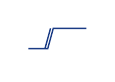
\begin{tikzpicture}[baseline=-.4ex,x=1em,y=1ex]\draw[color=blue,line width=.5pt] (0,0)--(.7,0)--(.9,1.7)--(2.1,1.7);\draw[color=blue,line width=.5pt] (.6,0)--(.8,1.7);\end{tikzpicture}}}{\par}{author paragraph instruction}{ps_134-4_043-v0009}If we dont assume
or know beforehand that W is strongly saturated, but just saturated say,
we may still introduce a more stringent compatibility condition, by
saying that \var{\xout{the}}{}{typewriter deletion}{ps_134-4_043-v0010} the homotopy structure h and W are \uline{strictly compatible}
if $W_h \hand{\subset} W$ . Using the \var{\xout{strict}}{}{typewriter deletion}{ps_134-4_043-v0011} saturation condition c') on W, it is easily
seen that in the case \var{\deleted{above}}{}{deletion}{ps_134-4_043-v0012} when h is a contractibility structure, \var{\deleted{and}}{}{deletion}{ps_134-4_043-v0013}
\var{\deleted{the functor $M \ W^{-1}M$ commutes to finite products,}}{}{deletion}{ps_134-4_043-v0014} then \var{\deleted{it is enough to}}{}{deletion}{ps_134-4_043-v0015} \var{\inserted{$W_h \subset W$ \deleted{\illegible{1}} (strict compa-%
tibility) is equivalent to: for}}{\hand{$W_h \subset W$  (strict compa-%
tibility) is equivalent to: for}}{insertion}{ps_134-4_043-v0016}
\var{\deleted{check that for}}{}{deletion}{ps_134-4_043-v0017} contractible X, the projection $X \hand{\to} e$ is \var{\xout{in W. \illegible{1}}}{}{typewriter deletion}{ps_134-4_043-v0018} \var{\inserted[typed]{"universally in W"}}{"universally in W"}{typed insertion}{ps_134-4_043-v0019}\hand{,}
\var{\inserted[typed]{or (as we'll say) W-\uline{aspheric}.}}{or (as we'll say) W-\uline{aspheric}.}{typed insertion}{ps_134-4_043-v0020}
Indeed, to deduce from this that any homotopism $f: X \hand{\to} Y$ is in W, we
are reduced to checking that any endomorphism of either X or Y which is
homotopic to the identity map, is in W. Now this will follow from the
assumption, and the following

\uline{Proposition} Assume the homotopy structure h on M can be defined by a
generating set $\hand{\Sigma}_h^o$ of weak homotopy intervals $\underline{I} =(I,\hand{\delta}_o,\hand{\delta}_1)$ which are
W-\uline{aspheric} (i.e. I W-aspheric over \var{\inserted{e}}{\hand{e}}{insertion}{ps_134-4_043-v0021}\var{\xout{\unsure{I}\illegible{1}}}{}{typewriter deletion}{ps_134-4_043-v0022} ), \var{\over{t}{w}}{\hand{w}}{writing over}{ps_134-4_043-v0023}\var{\over{h}{h}}{\hand{h}}{writing over}{ps_134-4_043-v0024}ere W \var{\xout{is}}{}{typewriter deletion}{ps_134-4_043-v0025}$\hand{\subset} F\var{\over{l}{\ell}}{\hand{\ell}}{writing over}{ps_134-4_043-v0026}(M)$ is \var{\inserted{any}}{\hand{any}}{insertion}{ps_134-4_043-v0027} saturated \var{\inserted{subset}}{\hand{subset}}{insertion}{ps_134-4_043-v0028}
(in fact, mildly saturated is enough). T$\overset{\hand{\scriptscriptstyle\perp\perp}}{\mathrm h}$en W is the inverse image \var{\xout{of}}{}{typewriter deletion}{ps_134-4_043-v0029}
by the canonical functor $M \hand{\to} M_h = \overline{M}$ of a \var{\xout{mildly}}{}{typewriter deletion}{ps_134-4_043-v0030} subset $\overline{W} \hand{\subset} F\var{\over{l}{\ell}}{\hand{\ell}}{writing over}{ps_134-4_043-v0031}(\overline{M})$, i.e.
\var{\xout{the relation}}{}{typewriter deletion}{ps_134-4_043-v0032} if f,g are homotopic arrows in M, if one is in W, so is the
other. Moreover (if W is saturated) $W_h \hand{\subset} W$ i.e. h and W are \var{\over{st}{st}}{\hand{st}}{writing over}{ps_134-4_043-v0033}rictly
compatible.

\margin{43}

%% END SOURCE ps_134-4_043
\ifnum\EditionMode=1
\psapparatusstart
\psentry{ps_134-4_043-v0001}{1}{typewriter deletion}{\xout{\unsure{sub}}}{}{The typewriter strikes out this material; it leaves the corrected running text.}
\psentry{ps_134-4_043-v0002}{2}{writing over}{$\over{l}{\ell}$}{$\hand{\ell}$}{The superposed handwritten reading replaces the underlying reading.}
\psentry{ps_134-4_043-v0003}{3}{typed insertion}{\inserted[typed]{it is with}}{it is with}{The typed insertion is incorporated at its indicated position; insertion brackets leave the running text.}
\psentry{ps_134-4_043-v0004}{4}{typewriter deletion}{\xout{is}}{}{The typewriter strikes out this material; it leaves the corrected running text.}
\psentry{ps_134-4_043-v0005}{5}{typewriter deletion}{\xout{this also means that the for}}{}{The typewriter strikes out this material; it leaves the corrected running text.}
\psentry{ps_134-4_043-v0006}{6}{writing over}{\over{\unsure{h}}{h}}{\hand{h}}{The superposed handwritten reading replaces the underlying reading.}
\psentry{ps_134-4_043-v0007}{7}{typewriter deletion}{\xout{this also}}{}{The typewriter strikes out this material; it leaves the corrected running text.}
\psentry{ps_134-4_043-v0008}{8}{slip corrected}{is is sufficient}{it is sufficient}{Isolated s for t in it is; the impersonal construction and correctly typed it is elsewhere in the reviewed discussion settle the slip.}
\psentry{ps_134-4_043-v0009}{9}{author paragraph instruction}{\diagram{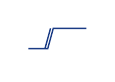
\begin{tikzpicture}[baseline=-.4ex,x=1em,y=1ex]\draw[color=blue,line width=.5pt] (0,0)--(.7,0)--(.9,1.7)--(2.1,1.7);\draw[color=blue,line width=.5pt] (.6,0)--(.8,1.7);\end{tikzpicture}}}{\par}{Apply the new paragraph before If we directed by the doubled stepped pen sign.}
\psentry{ps_134-4_043-v0010}{10}{typewriter deletion}{\xout{the}}{}{The typewriter strikes out this material; it leaves the corrected running text.}
\psentry{ps_134-4_043-v0011}{11}{typewriter deletion}{\xout{strict}}{}{The typewriter strikes out this material; it leaves the corrected running text.}
\psentry{ps_134-4_043-v0012}{12}{deletion}{\deleted{above}}{}{The author cancels this material by hand; it leaves the corrected running text.}
\psentry{ps_134-4_043-v0013}{13}{deletion}{\deleted{and}}{}{The author cancels this material by hand; it leaves the corrected running text.}
\psentry{ps_134-4_043-v0014}{14}{deletion}{\deleted{the functor $M \ W^{-1}M$ commutes to finite products,}}{}{The author cancels this material by hand; it leaves the corrected running text.}
\psentry{ps_134-4_043-v0015}{15}{deletion}{\deleted{it is enough to}}{}{The author cancels this material by hand; it leaves the corrected running text.}
\psentry{ps_134-4_043-v0016}{16}{insertion}{\inserted{$W_h \subset W$ \deleted{\illegible{1}} (strict compa-%
tibility) is equivalent to: for}}{\hand{$W_h \subset W$  (strict compa-%
tibility) is equivalent to: for}}{The handwritten insertion is incorporated at its indicated position; insertion brackets leave the running text.}
\psentry{ps_134-4_043-v0017}{17}{deletion}{\deleted{check that for}}{}{The author cancels this material by hand; it leaves the corrected running text.}
\psentry{ps_134-4_043-v0018}{18}{typewriter deletion}{\xout{in W. \illegible{1}}}{}{The typewriter strikes out this material; it leaves the corrected running text.}
\psentry{ps_134-4_043-v0019}{19}{typed insertion}{\inserted[typed]{"universally in W"}}{"universally in W"}{The typed insertion is incorporated at its indicated position; insertion brackets leave the running text.}
\psentry{ps_134-4_043-v0020}{20}{typed insertion}{\inserted[typed]{or (as we'll say) W-\uline{aspheric}.}}{or (as we'll say) W-\uline{aspheric}.}{The typed insertion is incorporated at its indicated position; insertion brackets leave the running text.}
\psentry{ps_134-4_043-v0021}{21}{insertion}{\inserted{e}}{\hand{e}}{The handwritten insertion is incorporated at its indicated position; insertion brackets leave the running text.}
\psentry{ps_134-4_043-v0022}{22}{typewriter deletion}{\xout{\unsure{I}\illegible{1}}}{}{The typewriter strikes out this material; it leaves the corrected running text.}
\psentry{ps_134-4_043-v0023}{23}{writing over}{\over{t}{w}}{\hand{w}}{The superposed handwritten reading replaces the underlying reading.}
\psentry{ps_134-4_043-v0024}{24}{writing over}{\over{h}{h}}{\hand{h}}{The superposed handwritten reading replaces the underlying reading.}
\psentry{ps_134-4_043-v0025}{25}{typewriter deletion}{\xout{is}}{}{The typewriter strikes out this material; it leaves the corrected running text.}
\psentry{ps_134-4_043-v0026}{26}{writing over}{$\over{l}{\ell}$}{$\hand{\ell}$}{The superposed handwritten reading replaces the underlying reading.}
\psentry{ps_134-4_043-v0027}{27}{insertion}{\inserted{any}}{\hand{any}}{The handwritten insertion is incorporated at its indicated position; insertion brackets leave the running text.}
\psentry{ps_134-4_043-v0028}{28}{insertion}{\inserted{subset}}{\hand{subset}}{The handwritten insertion is incorporated at its indicated position; insertion brackets leave the running text.}
\psentry{ps_134-4_043-v0029}{29}{typewriter deletion}{\xout{of}}{}{The typewriter strikes out this material; it leaves the corrected running text.}
\psentry{ps_134-4_043-v0030}{30}{typewriter deletion}{\xout{mildly}}{}{The typewriter strikes out this material; it leaves the corrected running text.}
\psentry{ps_134-4_043-v0031}{31}{writing over}{$\over{l}{\ell}$}{$\hand{\ell}$}{The superposed handwritten reading replaces the underlying reading.}
\psentry{ps_134-4_043-v0032}{32}{typewriter deletion}{\xout{the relation}}{}{The typewriter strikes out this material; it leaves the corrected running text.}
\psentry{ps_134-4_043-v0033}{33}{writing over}{\over{st}{st}}{\hand{st}}{The superposed handwritten reading replaces the underlying reading.}
\psapparatusend
\fi
\pssource{ps_134-4_061}{134-4/61}{https://grothendieck.umontpellier.fr/web/viewer.html?file=../134-4.pdf\#page=62}
\psnumber{ps_134-4_061-v0001}{1}
\psnumber{ps_134-4_061-v0002}{2}
\psnumber{ps_134-4_061-v0003}{3}
\psnumber{ps_134-4_061-v0004}{4}
\psnumber{ps_134-4_061-v0005}{5}
\psnumber{ps_134-4_061-v0006}{6}
\psnumber{ps_134-4_061-v0007}{7}
\psnumber{ps_134-4_061-v0008}{8}
\psnumber{ps_134-4_061-v0009}{9}
\psnumber{ps_134-4_061-v0010}{10}
\psnumber{ps_134-4_061-v0011}{11}
\psnumber{ps_134-4_061-v0012}{12}
%% BEGIN SOURCE ps_134-4_061
% Pursuing Stacks (cotes 134-2 to 134-8): archive cote 134-4, site page 61 (PDF page 62), typescript page 149.
% typescript. Draft compared: ps3.tex:3104-3168.
% AI-transcribed by Claude Opus 5.5 (claude-opus-5-5, adaptive thinking, effort high), Message Batches API, batch ps2 (msgbatch_01NVwr1Yuo8qJf5rykeGBXPK), 2026-11-12; reviewed against both supplied scan halves; see CHECK_DECISIONS.tsv.
\scanpage{134-4/61}
\mspage{149}

that the product of two elements in A be O-connected.  T\var{\over[typed]{h}{H}}{H}{typewriter overwriting}{ps_134-4_061-v0001}e topos is called
\uline{strictly} \uline{totally} O-\uline{con\var{\inserted{n}}{\hand{n}}{insertion}{ps_134-4_061-v0002}ected}  if it is locally connected,  and if moreover
every O-connected object admits a section  -  which (as we saw earlier to-%
day) implies \hand{$\mathcal{A}$} is totally O-connected,  as the wording suggests.  It
amounts to the same to demand that every ``non empty'' object have a section
-  and for this it is enough that the elements in A have a section.  This
latter condition is trivially checked for all standart test categories
I've met so far  (they all have a final object,  and there are maps of the
latter into any other object of A).  A noticeable counterexample here is
$(\hand{\Delta}^{\mathrm{f}})\hat{\ }$ (semisimplicial face complexes,  \uline{without} \uline{degeneracies}),  where \var{\xout{xx}}{}{typewriter deletion}{ps_134-4_061-v0003}
the \uline{weak} test category \hand{$\Delta$}$^{\mathrm{f}}$ hasnt got a final object  (\hand{$\Delta$}$_{\mathrm{o}}$ definitely
\margin{X} is'nt !)  and no \hand{$\Delta$}$_{\mathrm{n}}$ in \hand{$\Delta$}$^{\mathrm{f}}$ \var{\deleted{except \hand{$\Delta$}$_{\mathrm{o}}$ only}}{}{deletion}{ps_134-4_061-v0004} has got a section.

\uline{Remark}  I wonder,  when \var{\inserted{$\mathcal{A}$}}{\hand{$\mathcal{A}$}}{insertion}{ps_134-4_061-v0005} is totally O-connected, and moreover modelizing
i.e. the Lawvere element is aspheric over e ,  if this implies \hand{$\mathcal{A}$} is
totally aspheric,  and that every element  which is ``non empty'' has a
section (i.e. \uline{strict} total O-connectedness).  \var{\xout{At any rate, the}}{}{typewriter deletion}{ps_134-4_061-v0006}

Next thing is to look at
\[ W \subset \mathrm{F}\unsure{\mathrm{l}}(\hand{\mathcal{A}}) \]
the set of weak equivalences (as defined by non commutative cohomology
of topoi),  and see if it is ``geometric''(page 142).  Condition a') is \var{\xout{xxxx}}{}{typewriter deletion}{ps_134-4_061-v0007}
clearly satisfied,  there remains the condition b),  namely whether
O-connectedness of an object of \hand{$\mathcal{A}$} (\hand{$\mathcal{A}$} supposed totally O-connected) can
be tested,  using ``intervals'' which are \var{\xout{xx}}{}{typewriter deletion}{ps_134-4_061-v0008}\uline{aspheric over} e .  More specifi-%
cally,  we want to test that two sections of I belong to the same connec-%
ted component,  using for ``joining'' them intervals which are \var{\xout{xx}}{}{typewriter deletion}{ps_134-4_061-v0009}aspheric
over e .  The natural idea here is to assume the generating objects \hand{in $A$}
to be aspheric over e (which implies \hand{$\mathcal{A}$} is \uline{totally aspheric},  not only
totally O-connected),  and to use these objects (endowed with suitable
sections) as testing intervals.  This goes through smoothly indeed,  if
we assume  moreover strict total zero-connectedness.  Thus:

\uline{Proposition}  Let \hand{$\mathcal{A}$} be a topos which is strictly totally aspheric
(namely totally aspheric,  and every ``non empty'' object has a section)\hand{:}
\margin{\unsure{cf. lemme} p.268} Then the set W $\subset$ F\unsure{l}(\hand{$\mathcal{A}$})  of weak equivalences in \hand{$\mathcal{A}$} is ``geometric'' ,  and
accordingly,  the homotopy structure h$_{\mathrm{W}}$  defined in terms of aspheric
homotopy intervals,  is the same as the canonical homotopy structure h$_{\mathrm{M}}$
defined in terms of merely O-connected homotopy intervals.  \hand{Moreover, \var{\inserted{for}}{\hand{for}}{insertion}{ps_134-4_061-v0010} any
set $A \subset \mathrm{Ob}\,\mathcal{A}$ which is generating and whose objects are 0-connected,
the set of \var{\deleted{inter}}{}{deletion}{ps_134-4_061-v0011} 0-connected intervals \var{\deleted{in A}}{}{deletion}{ps_134-4_061-v0012} $\underline{I}=(I,\delta_0,\delta_1)$ with $I$
in $A$, generate the homotopy structure $h_W$.}

\margin{61}

%% END SOURCE ps_134-4_061
\ifnum\EditionMode=1
\psapparatusstart
\psentry{ps_134-4_061-v0001}{1}{typewriter overwriting}{\over[typed]{h}{H}}{H}{The superposed typed reading replaces the underlying reading.}
\psentry{ps_134-4_061-v0002}{2}{insertion}{\inserted{n}}{\hand{n}}{The handwritten insertion is incorporated at its indicated position; insertion brackets leave the running text.}
\psentry{ps_134-4_061-v0003}{3}{typewriter deletion}{\xout{xx}}{}{The typewriter strikes out this material; it leaves the corrected running text.}
\psentry{ps_134-4_061-v0004}{4}{deletion}{\deleted{except \hand{$\Delta$}$_{\mathrm{o}}$ only}}{}{The author cancels this material by hand; it leaves the corrected running text.}
\psentry{ps_134-4_061-v0005}{5}{insertion}{\inserted{$\mathcal{A}$}}{\hand{$\mathcal{A}$}}{The handwritten insertion is incorporated at its indicated position; insertion brackets leave the running text.}
\psentry{ps_134-4_061-v0006}{6}{typewriter deletion}{\xout{At any rate, the}}{}{The typewriter strikes out this material; it leaves the corrected running text.}
\psentry{ps_134-4_061-v0007}{7}{typewriter deletion}{\xout{xxxx}}{}{The typewriter strikes out this material; it leaves the corrected running text.}
\psentry{ps_134-4_061-v0008}{8}{typewriter deletion}{\xout{xx}}{}{The typewriter strikes out this material; it leaves the corrected running text.}
\psentry{ps_134-4_061-v0009}{9}{typewriter deletion}{\xout{xx}}{}{The typewriter strikes out this material; it leaves the corrected running text.}
\psentry{ps_134-4_061-v0010}{10}{insertion}{\inserted{for}}{\hand{for}}{The handwritten insertion is incorporated at its indicated position; insertion brackets leave the running text.}
\psentry{ps_134-4_061-v0011}{11}{deletion}{\deleted{inter}}{}{The author cancels this material by hand; it leaves the corrected running text.}
\psentry{ps_134-4_061-v0012}{12}{deletion}{\deleted{in A}}{}{The author cancels this material by hand; it leaves the corrected running text.}
\psapparatusend
\fi
\pssource{ps_134-4_062}{134-4/62}{https://grothendieck.umontpellier.fr/web/viewer.html?file=../134-4.pdf\#page=63}
\psnumber{ps_134-4_062-v0001}{1}
\psnumber{ps_134-4_062-v0002}{2}
\psnumber{ps_134-4_062-v0003}{3}
\psnumber{ps_134-4_062-v0004}{4}
\psnumber{ps_134-4_062-v0005}{5}
\psnumber{ps_134-4_062-v0006}{6}
\psnumber{ps_134-4_062-v0007}{7}
\psnumber{ps_134-4_062-v0008}{8}
\psnumber{ps_134-4_062-v0009}{9}
\psnumber{ps_134-4_062-v0010}{10}
\psnumber{ps_134-4_062-v0011}{11}
\psnumber{ps_134-4_062-v0012}{12}
%% BEGIN SOURCE ps_134-4_062
% Pursuing Stacks (cotes 134-2 to 134-8): archive cote 134-4, site page 62 (PDF page 63), typescript page 150.
% typescript. Draft compared: ps3.tex:3153-3218.
% AI-transcribed by Claude Opus 5.5 (claude-opus-5-5, adaptive thinking, effort high), Message Batches API, batch ps2 (msgbatch_01NVwr1Yuo8qJf5rykeGBXPK), 2026-11-12; reviewed against both supplied scan halves; see CHECK_DECISIONS.tsv.
\scanpage{134-4/62}
\mspage{150}

A topos \hand{$\mathcal{A}$} as in the proposition (namely strictly totally aspheric)
need not be \var{\deleted{a}}{}{deletion}{ps_134-4_062-v0001} modeliz\var{\over{er}{ing}}{\hand{ing}}{writing over}{ps_134-4_062-v0002}, i.e. \var{\xout{xxxxxxxx}}{}{typewriter deletion}{ps_134-4_062-v0003} the Lawvere element L need not
be aspheric, or what amounts to the same because of $h_W = h_M$ and L being
\margin{x} a \uwave{contrac}tor, L need not be connected: take \hand{$\mathcal{A}$} = (Sets) ! I suspect
\margin{X} though this to be the only counterexample (up to equivalence)\hand{(*)}.For \hand{$\mathcal{A}$} to
be a modelizer, we need only find an object in A which has got two
\uline{distinct} sections (because then \unsure{they|thay} must be disjoint i.e. $e_0 \wedge e_1 = \emptyset_{\hand{\mathcal{A}}}$ ,
because e has only the full and the ``empty'' subobject, as a consequence
of every ``non empty'' object of \hand{$\mathcal{A}$} having a section), thus getting a
``homotopy interval'' (more specifically, a \var{\inserted[typed]{separated and}}{separated and}{typed insertion}{ps_134-4_062-v0004} relatively aspheric \var{\xout{and}}{}{typewriter deletion}{ps_134-4_062-v0005} A one)
as requested for \hand{$\mathcal{A}$} to be a modelizer. Now for any \var{\inserted[typed]{would-be}}{would-be}{typed insertion}{ps_134-4_062-v0006} test category met
with so far (except precisely \hand{$\Delta$}$^f$ and the like, which are \var{\xout{xxxx}}{}{typewriter deletion}{ps_134-4_062-v0007} \uline{not}
test categories but only weak ones), this condition that there are objects
in A which have more than just one``point''\var{\xout{xx}}{}{typewriter deletion}{ps_134-4_062-v0008} \hand{(}\var{\xout{i.e.}}{}{typewriter deletion}{ps_134-4_062-v0009}= section\hand{)}, is trivially
verified.

In case of a topos of the type A\^{}, the notion of weak equivalence in
A\^{} can be described (independently of cohomological notions) in terms of
the notion of weak equivalence in (Cat), more precisely
\[ W_A \overset{\text{def}}{=} W_{A\hat{}} = i_A^{-1}(\underline{W}) , \]
where
\[ i_A :\ A\hat{} \hand{\to} (\mathrm{Cat}) , \quad F \hand{\mapsto} A_{/F} \]
is the canonical functor, and where
\[ \underline{W} = W_{(\mathrm{Cat})} \]
is the set of weak equivalences in (Cat). These of \unsure{course|dourse}, for the time
being, are defined in terms of \var{\xout{(non commutative)}}{}{typewriter deletion}{ps_134-4_062-v0010} cohomology (including
a bit of non commutative one in dimension\var{\xout{s}}{}{typewriter deletion}{ps_134-4_062-v0011} 1 ...). We may however start
with any $\underline{W} \subset Fl((\mathrm{Cat}))$ and look at which formal properties on $\underline{W}$ (satis-%
fied for usual weak equivalences) allow our arguments to go through, in
various circumstances. We may make a list of those which have been used
today, and go on this way a little longer, with the expectation we'll
finally wind up with an axiomatic characterization of weak equivalences
i.e. of $\underline{W}$,in terms of the category (Cat)\var{\xout{,}}{}{typewriter deletion}{ps_134-4_062-v0012} say.
a) (Pour mémoire !) $\underline{W}$ is saturated (cf. page 101).
b) $\underline{W}$ is 0-admissible , i.e. if f: C $\hand{\to}$ C' is in $\underline{W}$ , $\hand{\pi}_0$(f) is bijective

c) $\hand{\Delta}_1$ is $\underline{W}$-aspheric over e = $\hand{\Delta}_0$ , i.e. for every C in (Cat), the
projection C x$\hand{\Delta}_1 \hand{\longrightarrow}$ C is in $\underline{W}$ .
d) Any C in (Cat) which has a final element is $\underline{W}$-aspheric i.e.
C $\hand{\to}$ e is in $\underline{W}$ .

\margin{62}

%% END SOURCE ps_134-4_062
\ifnum\EditionMode=1
\psapparatusstart
\psentry{ps_134-4_062-v0001}{1}{deletion}{\deleted{a}}{}{The author cancels this material by hand; it leaves the corrected running text.}
\psentry{ps_134-4_062-v0002}{2}{writing over}{\over{er}{ing}}{\hand{ing}}{The superposed handwritten reading replaces the underlying reading.}
\psentry{ps_134-4_062-v0003}{3}{typewriter deletion}{\xout{xxxxxxxx}}{}{The typewriter strikes out this material; it leaves the corrected running text.}
\psentry{ps_134-4_062-v0004}{4}{typed insertion}{\inserted[typed]{separated and}}{separated and}{The typed insertion is incorporated at its indicated position; insertion brackets leave the running text.}
\psentry{ps_134-4_062-v0005}{5}{typewriter deletion}{\xout{and}}{}{The typewriter strikes out this material; it leaves the corrected running text.}
\psentry{ps_134-4_062-v0006}{6}{typed insertion}{\inserted[typed]{would-be}}{would-be}{The typed insertion is incorporated at its indicated position; insertion brackets leave the running text.}
\psentry{ps_134-4_062-v0007}{7}{typewriter deletion}{\xout{xxxx}}{}{The typewriter strikes out this material; it leaves the corrected running text.}
\psentry{ps_134-4_062-v0008}{8}{typewriter deletion}{\xout{xx}}{}{The typewriter strikes out this material; it leaves the corrected running text.}
\psentry{ps_134-4_062-v0009}{9}{typewriter deletion}{\xout{i.e.}}{}{The typewriter strikes out this material; it leaves the corrected running text.}
\psentry{ps_134-4_062-v0010}{10}{typewriter deletion}{\xout{(non commutative)}}{}{The typewriter strikes out this material; it leaves the corrected running text.}
\psentry{ps_134-4_062-v0011}{11}{typewriter deletion}{\xout{s}}{}{The typewriter strikes out this material; it leaves the corrected running text.}
\psentry{ps_134-4_062-v0012}{12}{typewriter deletion}{\xout{,}}{}{The typewriter strikes out this material; it leaves the corrected running text.}
\psapparatusend
\fi
\pssource{ps_134-4_063}{134-4/63}{https://grothendieck.umontpellier.fr/web/viewer.html?file=../134-4.pdf\#page=64}
\psnumber{ps_134-4_063-v0001}{1}
\psnumber{ps_134-4_063-v0002}{2}
\psnumber{ps_134-4_063-v0003}{3}
\psnumber{ps_134-4_063-v0004}{4}
\psnumber{ps_134-4_063-v0005}{5}
\psnumber{ps_134-4_063-v0006}{6}
\psnumber{ps_134-4_063-v0007}{7}
\psnumber{ps_134-4_063-v0008}{8}
\psnumber{ps_134-4_063-v0009}{9}
\psnumber{ps_134-4_063-v0010}{10}
\psnumber{ps_134-4_063-v0011}{11}
\psnumber{ps_134-4_063-v0012}{12}
\psnumber{ps_134-4_063-v0013}{13}
\psnumber{ps_134-4_063-v0014}{14}
\psnumber{ps_134-4_063-v0015}{15}
\psnumber{ps_134-4_063-v0016}{16}
%% BEGIN SOURCE ps_134-4_063
% Pursuing Stacks (cotes 134-2 to 134-8): archive cote 134-4, site page 63 (PDF page 64), typescript page 151.
% typescript. Draft compared: ps3.tex:3201-3278.
% AI-transcribed by Claude Opus 5.5 (claude-opus-5-5, adaptive thinking, effort high), Message Batches API, batch ps2 (msgbatch_01NVwr1Yuo8qJf5rykeGBXPK), 2026-11-12; reviewed against both supplied scan halves; see CHECK_DECISIONS.tsv.
\scanpage{134-4/63}
\mspage{151}

T\var{\over[typed]{h}{\unsure{H|h}}}{\unsure{H|h}}{typewriter overwriting}{ps_134-4_063-v0001}e condition a) will be tacitly understood throughout, when taking
a $\underline{W}$ to replace usual weak equivalences. Conditions b) and c) \var{\inserted{then}}{\hand{then}}{insertion}{ps_134-4_063-v0002} were seen to
be enough to imply that $h_{\underline{W}} = h_{(Cat)}$ . On the other hand, one sees at
once that for the proposition above for a \var{\xout{topos A}}{}{typewriter deletion}{ps_134-4_063-v0003} topos $A\hat{}$ \var{\xout{of the typ}}{}{typewriter deletion}{ps_134-4_063-v0004}\hand{wh}ich
is strictly totally aspheric, when we define now $\underline{W}_A \subset \mathrm{F}\var{\over{l}{\ell}}{\hand{\ell}}{writing over}{ps_134-4_063-v0005}(A\hand{\hat{}}\ )$ as just
$i_A^{-1}(\underline{W})$ , in order to conclude $h_{(\underline{W}_A)} = h_{A\hat{}}$ , all we made use of was
(besides saturation of $\underline{W}$ of course i.e. a)) b) and d).

O\var{\over[typed]{n}{\unsure{H|n}}}{\unsure{H|n}}{typewriter overwriting}{ps_134-4_063-v0006}e may object that d) is'nt expressed in terms of the category
structure of (Cat) only, but we could express it in terms of this struc-%
ture, by the remark that C has a final object iff there exists a\var{\xout{n}}{}{typewriter deletion}{ps_134-4_063-v0007}
$\hand{\Delta}^1$-homotopy of $id_C$ to a constant section of C (this ``section'' will indeed
be defined necessarily by a final object of C). As was to be expected,
in this formulation, as in c) too, the object $\hand{\Delta}_1$ of (Cat) is playing a
crucial role. But at this point i\var{\over{t}{t}}{\hand{t}}{writing over}{ps_134-4_063-v0008} occurs to me that c) implies d),
by the homotopy lemma - thus for the time being all we needed was
a)b)c).

\var{\over{6}{6}}{\hand{6}}{writing over}{ps_134-4_063-v0009}\var{\over{8}{1}}{\hand{1}}{writing over}{ps_134-4_063-v0010}. We now in the long last get back to the ``key result'' promised time
ago, and which we kept pushing off. To pay off the trouble of the long
digression in between, maybe it'll come out more smoothly. It shall be
concerned with a functor
\[ (1) \qquad i : A \hand{\longrightarrow} (Cat) \quad , \]
where in the end A will be (or turn out to be) a strict test category,
and we want to give characterizations for i to be a \var{\inserted{(weak)}}{\hand{(weak)}}{insertion}{ps_134-4_063-v0011} test functor, namely
the corresponding functor
\[ (2) \qquad i^{*} : (Cat) \hand{\longrightarrow} A\hat{} \]
to induce an equivalence between the localizations, with respect to
``weak equivalences''.\hand{*} We'll now be a little more demanding, and instead \margin{* Plus a little more, see below (8).}
of just assuming it is the usual notion of weak equivalence either in (Cat\hand{)}
or in $\var{\over{A}{A}}{\hand{A}}{writing over}{ps_134-4_063-v0012}\hat{}$, I'll assume that the set $\underline{W}_A \subset \mathrm{F1}(A\hat{})$ is defined in terms of
a saturated \var{\xout{sub}}{}{typewriter deletion}{ps_134-4_063-v0013}set $\underline{W} \subset \mathrm{F}\var{\over{l}{\ell}}{\hand{\ell}}{writing over}{ps_134-4_063-v0014}((Cat))$ of arrows in \hand{(}Cat) , by taking the invers
% NOTE: the right edge of the scan cuts the end of this line ("invers")
image by the functor
\[ (3) \qquad i_A : A\hat{} \hand{\rightarrow} (Cat) \]
as above, whereas in the target category (Cat) of (2), we'll work
with another saturated set $\underline{W}'$ - thus besides \var{\over{\unsure{(}}{(}}{\hand{(}}{writing over}{ps_134-4_063-v0015}1), the data are more-%
over
\[ (4) \qquad \underline{W} \ , \ \underline{W}' \subset \mathrm{F}\var{\over{l}{\ell}}{\hand{\ell}}{writing over}{ps_134-4_063-v0016}(Cat)) \qquad , \]

\margin{63}

%% END SOURCE ps_134-4_063
\ifnum\EditionMode=1
\psapparatusstart
\psentry{ps_134-4_063-v0001}{1}{typewriter overwriting}{\over[typed]{h}{\unsure{H|h}}}{\unsure{H|h}}{The superposed typed reading replaces the underlying reading.}
\psentry{ps_134-4_063-v0002}{2}{insertion}{\inserted{then}}{\hand{then}}{The handwritten insertion is incorporated at its indicated position; insertion brackets leave the running text.}
\psentry{ps_134-4_063-v0003}{3}{typewriter deletion}{\xout{topos A}}{}{The typewriter strikes out this material; it leaves the corrected running text.}
\psentry{ps_134-4_063-v0004}{4}{typewriter deletion}{\xout{of the typ}}{}{The typewriter strikes out this material; it leaves the corrected running text.}
\psentry{ps_134-4_063-v0005}{5}{writing over}{$\over{l}{\ell}$}{$\hand{\ell}$}{The superposed handwritten reading replaces the underlying reading.}
\psentry{ps_134-4_063-v0006}{6}{typewriter overwriting}{\over[typed]{n}{\unsure{H|n}}}{\unsure{H|n}}{The superposed typed reading replaces the underlying reading.}
\psentry{ps_134-4_063-v0007}{7}{typewriter deletion}{\xout{n}}{}{The typewriter strikes out this material; it leaves the corrected running text.}
\psentry{ps_134-4_063-v0008}{8}{writing over}{\over{t}{t}}{\hand{t}}{The superposed handwritten reading replaces the underlying reading.}
\psentry{ps_134-4_063-v0009}{9}{writing over}{\over{6}{6}}{\hand{6}}{The superposed handwritten reading replaces the underlying reading.}
\psentry{ps_134-4_063-v0010}{10}{writing over}{\over{8}{1}}{\hand{1}}{The superposed handwritten reading replaces the underlying reading.}
\psentry{ps_134-4_063-v0011}{11}{insertion}{\inserted{(weak)}}{\hand{(weak)}}{The handwritten insertion is incorporated at its indicated position; insertion brackets leave the running text.}
\psentry{ps_134-4_063-v0012}{12}{writing over}{$\over{A}{A}$}{$\hand{A}$}{The superposed handwritten reading replaces the underlying reading.}
\psentry{ps_134-4_063-v0013}{13}{typewriter deletion}{\xout{sub}}{}{The typewriter strikes out this material; it leaves the corrected running text.}
\psentry{ps_134-4_063-v0014}{14}{writing over}{$\over{l}{\ell}$}{$\hand{\ell}$}{The superposed handwritten reading replaces the underlying reading.}
\psentry{ps_134-4_063-v0015}{15}{writing over}{\over{\unsure{(}}{(}}{\hand{(}}{The superposed handwritten reading replaces the underlying reading.}
\psentry{ps_134-4_063-v0016}{16}{writing over}{$\over{l}{\ell}$}{$\hand{\ell}$}{The superposed handwritten reading replaces the underlying reading.}
\psapparatusend
\fi
\pssource{ps_134-4_064}{134-4/64}{https://grothendieck.umontpellier.fr/web/viewer.html?file=../134-4.pdf\#page=65}
\psnumber{ps_134-4_064-v0001}{1}
\psnumber{ps_134-4_064-v0002}{2}
\psnumber{ps_134-4_064-v0003}{3}
\psnumber{ps_134-4_064-v0004}{4}
\psnumber{ps_134-4_064-v0005}{5}
\psnumber{ps_134-4_064-v0006}{6}
\psnumber{ps_134-4_064-v0007}{7}
%% BEGIN SOURCE ps_134-4_064
% Pursuing Stacks (cotes 134-2 to 134-8): archive cote 134-4, site page 64 (PDF page 65), typescript page 152.
% typescript. Draft compared: ps3.tex:3258-3343.
% AI-transcribed by Claude Opus 5.5 (claude-opus-5-5, adaptive thinking, effort high), Message Batches API, batch ps2 (msgbatch_01NVwr1Yuo8qJf5rykeGBXPK), 2026-11-12; reviewed against both supplied scan halves; see CHECK_DECISIONS.tsv.
\scanpage{134-4/64}
\mspage{152}
two saturated sets of arrows in (Cat), with no special assumption other-%
wise for the time being. We will introduce the properties we need on
these, as well as on A and on i, stepwise as the situation will tell us.
We want to derive a set of conditions insuring that both (2) and (3)
induce equivalences for the respective localizations, namely
\[ (5) \qquad \overline{i}^{*} : \underline{W}\hand{'}^{-1}(\mathrm{Cat}) \hand{\xrightarrow{\approx}} \underline{W}_A^{-1}A\hat{} \quad\text{and}\quad \overline{i}_A : \underline{W}_A^{-1}A\hat{} \hand{\xrightarrow{\approx}} \underline{W}^{-1}(\mathrm{Cat}) \qquad . \]
We may assume beforehand that A is a weak test category (``with respect to
$\underline{W}$ '' ) and hence the second functor in (5) is already an equivalence,
in which case the condition that the first functor in (5) exist and be an
equivalence (existence just meaning the condition
\[ (*) \qquad \underline{W}' \subset i^{* -1}(W_A) \qquad \text{i.e.} \quad i^{*}(\underline{W}') \subset W_A \quad ) \]
is equivalent to the \var{\inserted[typed]{corresponding}}{corresponding}{typed insertion}{ps_134-4_064-v0001} requirement for the composition
\[ (6) \qquad f_{\hand{i}} : (\mathrm{Cat}) \mathrel{\overset{i^{*}}{\hand{\longrightarrow}}} \var{\over{\unsure{A}}{A}}{\hand{A}}{writing over}{ps_134-4_064-v0002}\hat{} \mathrel{\overset{i_A}{\hand{\longrightarrow}}} (\mathrm{Cat}) \qquad , \]
namely that this induce an equivalence
\[ (7) \qquad \underline{W}'^{-1}(\mathrm{Cat}) \hand{\xrightarrow{\approx}} \underline{W}^{-1}(\mathrm{Cat}) \qquad . \]
As a matter of fact, we are going to be slightly more demanding (in ac-%
cordance with the notion of a \var{\inserted{weak}}{\hand{weak}}{insertion}{ps_134-4_064-v0003} test functor as developped previously,
cf. page \hand{85} ), namely that the inclusion (*) be in fact an equality
\[ (8) \qquad \underline{W}' = i^{* -1}(\underline{W}_A) \quad , \]
the similar requirement for the functor $i_A$ (3) being satisfied by the
very definition of $\underline{W}_A$ in terms of $\underline{W}$ as
\[ (9) \qquad \underline{W}_A = i_A^{-1}(\underline{W}) \quad . \]
In view of this, the extra requirement (8) boils down to the equivalent
requirement in terms of the composition $f_{\hand{i}}$ (6) :
\[ (10) \qquad \underline{W}' = f_{\hand{i}}^{-1}(\underline{W}) \quad . \]

To sum up, we want at least develop sufficient conditions on the
data ($\underline{W}$,$\underline{W}'$,A,i) for (8) to hold (which allows to define the first
functor in (5) , whereas the second is always defined), and the functors
in (5) to be equivalences; or equivalently, for (10) to hold, hence
a functor (7), and for the latter to be an equivalence\hand{,} and \var{\xout{A to be a}}{}{typewriter deletion}{ps_134-4_064-v0004}
\var{\xout{weak test category with respect to}}{}{typewriter deletion}{ps_134-4_064-v0005} equally $i_A$ to induce an equivalence
for the localizations (i.e. the second functor (5) an\var{\deleted{d}}{}{deletion}{ps_134-4_064-v0006} equivalence).
It should be noted that the latter condition depends only on (A,$\underline{W}$), not
on i nor on $\underline{W}'$ - it will be satisfied automatically if we assume A to
be a \uline{weak} \uline{test category} relative to $\underline{W}$ (namely \var{\xout{\illegible{1}}}{}{typewriter deletion}{ps_134-4_064-v0007}

\margin{64}

%% END SOURCE ps_134-4_064
\ifnum\EditionMode=1
\psapparatusstart
\psentry{ps_134-4_064-v0001}{1}{typed insertion}{\inserted[typed]{corresponding}}{corresponding}{The typed insertion is incorporated at its indicated position; insertion brackets leave the running text.}
\psentry{ps_134-4_064-v0002}{2}{writing over}{$\over{\unsure{A}}{A}$}{$\hand{A}$}{The superposed handwritten reading replaces the underlying reading.}
\psentry{ps_134-4_064-v0003}{3}{insertion}{\inserted{weak}}{\hand{weak}}{The handwritten insertion is incorporated at its indicated position; insertion brackets leave the running text.}
\psentry{ps_134-4_064-v0004}{4}{typewriter deletion}{\xout{A to be a}}{}{The typewriter strikes out this material; it leaves the corrected running text.}
\psentry{ps_134-4_064-v0005}{5}{typewriter deletion}{\xout{weak test category with respect to}}{}{The typewriter strikes out this material; it leaves the corrected running text.}
\psentry{ps_134-4_064-v0006}{6}{deletion}{\deleted{d}}{}{The author cancels this material by hand; it leaves the corrected running text.}
\psentry{ps_134-4_064-v0007}{7}{typewriter deletion}{\xout{\illegible{1}}}{}{The typewriter strikes out this material; it leaves the corrected running text.}
\psapparatusend
\fi
\pssource{ps_134-4_065}{134-4/65}{https://grothendieck.umontpellier.fr/web/viewer.html?file=../134-4.pdf\#page=66}
\psnumber{ps_134-4_065-v0001}{1}
\psnumber{ps_134-4_065-v0002}{2}
\psnumber{ps_134-4_065-v0003}{3}
\psnumber{ps_134-4_065-v0004}{4}
\psnumber{ps_134-4_065-v0005}{5}
\psnumber{ps_134-4_065-v0006}{6}
\psnumber{ps_134-4_065-v0007}{7}
\psnumber{ps_134-4_065-v0008}{8}
\psnumber{ps_134-4_065-v0009}{9}
\psnumber{ps_134-4_065-v0010}{10}
\psnumber{ps_134-4_065-v0011}{11}
\psnumber{ps_134-4_065-v0012}{12}
\psnumber{ps_134-4_065-v0013}{13}
\psnumber{ps_134-4_065-v0014}{14}
\psnumber{ps_134-4_065-v0015}{15}
\psnumber{ps_134-4_065-v0016}{16}
\psnumber{ps_134-4_065-v0017}{17}
\psnumber{ps_134-4_065-v0018}{18}
\psnumber{ps_134-4_065-v0019}{19}
\psnumber{ps_134-4_065-v0020}{20}
\psnumber{ps_134-4_065-v0021}{21}
%% BEGIN SOURCE ps_134-4_065
% Pursuing Stacks (cotes 134-2 to 134-8): archive cote 134-4, site page 65 (PDF page 66), typescript page 153.
% typescript. Draft compared: ps3.tex:3331-3394.
% AI-transcribed by Claude Opus 5.5 (claude-opus-5-5, adaptive thinking, effort high), Message Batches API, batch ps2 (msgbatch_01NVwr1Yuo8qJf5rykeGBXPK), 2026-11-12; reviewed against both supplied scan halves; see CHECK_DECISIONS.tsv.
\scanpage{134-4/65}
\mspage{153}

$i_A$ and the \var{\xout{functor}}{}{typewriter deletion}{ps_134-4_065-v0001} right adjoint functor
\[ j_A : (\mathrm{Cat}) \hand{\longrightarrow} A\hat{} \]
to induce quasi-inverse \var{\xout{localiz}}{}{typewriter deletion}{ps_134-4_065-v0002} equivalences for the localizations
$W_A^{-1}A\hat{}$ and $\underline{W}^{-1}(\mathrm{Cat})$ ). We have already developped handy ns conditions
for this in case $\underline{W} = W_{(\mathrm{Cat})}$ - and it would be easy enough to look up
which \var{\over{f}{f}}{\hand{f}}{writing over}{ps_134-4_065-v0003}ormal properties exactly on $W_{(\mathrm{Cat})}$ have been used in the proof,
if need be. At any rate, we know beforehand that we can find $(A,\underline{W})$
such that A be a \var{\inserted[typed]{weak}}{weak}{typed insertion}{ps_134-4_065-v0004} \var{\deleted{\illegible{1}}}{}{deletion}{ps_134-4_065-v0005}test category (and even a strict test category !) rela-%
tive to $\underline{W}$ . When $(A,\underline{W})$ are chosen this way beforehand, the question
just amounts to find\var{\inserted[typed]{ing}}{ing}{typed insertion}{ps_134-4_065-v0006} conditions \var{\xout{for (10) to}}{}{typewriter deletion}{ps_134-4_065-v0007} on $(\underline{W}',i)$ for (10) to hold
and for (7) to be an equivalence of categories. If we find conditions
which actually can be met, than we get as a by\hand{-}product the formula (10)
precisely, which says that \var{\xout{\illegible{2}}}{}{typewriter deletion}{ps_134-4_065-v0008} \var{\inserted[typed]{there is just \uline{one} $\underline{W}'$}}{there is just \uline{one} $\underline{W}'$}{typed insertion}{ps_134-4_065-v0009} satisfying the conditions\var{\xout{,\illegible{1}}}{}{typewriter deletion}{ps_134-4_065-v0010} on
$\underline{W}'$ , namely $f_i^{-1}(\underline{W})$ ! Of course, taking $\underline{W}$ \var{\deleted{\xout{to be just $W_{(\mathrm{Cat})}$ and it is}}}{}{deletion}{ps_134-4_065-v0011}
\var{\deleted{\xout{be and $\underline{W}'$}}}{}{deletion}{ps_134-4_065-v0012} to be just $W_{(\mathrm{Cat})}$ , it will follow surely that $\underline{W}'$ is just
$W_{(\mathrm{Cat})}$ - i.e. we should get an axiomatic characterization of weak equiva-%
-lences.

Let's now go to work, following the idea described in par. \var{\over{4}{5}}{\hand{5}}{writing over}{ps_134-4_065-v0013}7
(pages 96 -98), and expressed mainly in the basic diagram of canonical
maps in (Cat) , associated to a given object \var{\inserted{C}}{\hand{C}}{insertion}{ps_134-4_065-v0014} in (Cat):
\diagram{
(11)\qquad
\begin{tikzcd}[every arrow/.append style={draw=blue!65!black}]
A_{/C} \arrow[r] \& A_{//C} \& \\
 \& A\mathrm{x}C \arrow[u] \arrow[r] \& A
\end{tikzcd} \quad ,
}
which will allow to compare $f_i(C) = A_{/C}$ with C. When $\underline{W}\var{\deleted{'}}{}{deletion}{ps_134-4_065-v0015} = W_{(\mathrm{Cat})}$, it
was seen in loc. cit. that the two latter among these three\var{\xout{x}}{}{typewriter deletion}{ps_134-4_065-v0016} arrows
are in $\underline{W}$ , \var{\xout{\unsure{and we were a}}}{}{typewriter deletion}{ps_134-4_065-v0017} provided (for the middle one) we assume that
i takes it's values in the subcategory of (Cat) of all contractible cate-%
gories. What remained to be done, for getting the conditions for $f_i$ to
be ``weakly equivalent'' to the identity functor (and hence induce an equi-%
valence for the localizations) was to write down conditions for the
first functor in (11), $A_{/C} \hand{\to} A_{//C}$ , to be in $\underline{W}$ . We have moreover to
be explicit on the conditions to put on a general $\underline{W}$ , in order for the
two la\var{\over{tter}{st}}{\hand{st}}{writing over}{ps_134-4_065-v0018} maps in (11) to be in $\underline{W}$ . For the last functor, this conditi-%
on as a matter of fact involves both A and $\underline{W}$ , it is clearly equivalent
to

W 1) A is $\underline{W}$ - aspheric over e \hand{\unsure{;}}

\var{\over{i}{I}}{\hand{I}}{writing over}{ps_134-4_065-v0019}f we assume that A has a final element, this condition is \var{\xout{the consequence}}{}{typewriter deletion}{ps_134-4_065-v0020}
satisfied provided $\underline{W}$ satisfies the \var{\deleted{following}}{}{deletion}{ps_134-4_065-v0021} condition (where there is

\margin{65}

%% END SOURCE ps_134-4_065
\ifnum\EditionMode=1
\psapparatusstart
\psentry{ps_134-4_065-v0001}{1}{typewriter deletion}{\xout{functor}}{}{The typewriter strikes out this material; it leaves the corrected running text.}
\psentry{ps_134-4_065-v0002}{2}{typewriter deletion}{\xout{localiz}}{}{The typewriter strikes out this material; it leaves the corrected running text.}
\psentry{ps_134-4_065-v0003}{3}{writing over}{\over{f}{f}}{\hand{f}}{The superposed handwritten reading replaces the underlying reading.}
\psentry{ps_134-4_065-v0004}{4}{typed insertion}{\inserted[typed]{weak}}{weak}{The typed insertion is incorporated at its indicated position; insertion brackets leave the running text.}
\psentry{ps_134-4_065-v0005}{5}{deletion}{\deleted{\illegible{1}}}{}{The author cancels this material by hand; it leaves the corrected running text.}
\psentry{ps_134-4_065-v0006}{6}{typed insertion}{\inserted[typed]{ing}}{ing}{The typed insertion is incorporated at its indicated position; insertion brackets leave the running text.}
\psentry{ps_134-4_065-v0007}{7}{typewriter deletion}{\xout{for (10) to}}{}{The typewriter strikes out this material; it leaves the corrected running text.}
\psentry{ps_134-4_065-v0008}{8}{typewriter deletion}{\xout{\illegible{2}}}{}{The typewriter strikes out this material; it leaves the corrected running text.}
\psentry{ps_134-4_065-v0009}{9}{typed insertion}{\inserted[typed]{there is just \uline{one} $\underline{W}'$}}{there is just \uline{one} $\underline{W}'$}{The typed insertion is incorporated at its indicated position; insertion brackets leave the running text.}
\psentry{ps_134-4_065-v0010}{10}{typewriter deletion}{\xout{,\illegible{1}}}{}{The typewriter strikes out this material; it leaves the corrected running text.}
\psentry{ps_134-4_065-v0011}{11}{deletion}{\deleted{\xout{to be just $W_{(\mathrm{Cat})}$ and it is}}}{}{The author cancels this material by hand; it leaves the corrected running text.}
\psentry{ps_134-4_065-v0012}{12}{deletion}{\deleted{\xout{be and $\underline{W}'$}}}{}{The author cancels this material by hand; it leaves the corrected running text.}
\psentry{ps_134-4_065-v0013}{13}{writing over}{\over{4}{5}}{\hand{5}}{The superposed handwritten reading replaces the underlying reading.}
\psentry{ps_134-4_065-v0014}{14}{insertion}{\inserted{C}}{\hand{C}}{The handwritten insertion is incorporated at its indicated position; insertion brackets leave the running text.}
\psentry{ps_134-4_065-v0015}{15}{deletion}{$\deleted{'}$}{}{The author cancels this material by hand; it leaves the corrected running text.}
\psentry{ps_134-4_065-v0016}{16}{typewriter deletion}{\xout{x}}{}{The typewriter strikes out this material; it leaves the corrected running text.}
\psentry{ps_134-4_065-v0017}{17}{typewriter deletion}{\xout{\unsure{and we were a}}}{}{The typewriter strikes out this material; it leaves the corrected running text.}
\psentry{ps_134-4_065-v0018}{18}{writing over}{\over{tter}{st}}{\hand{st}}{The superposed handwritten reading replaces the underlying reading.}
\psentry{ps_134-4_065-v0019}{19}{writing over}{\over{i}{I}}{\hand{I}}{The superposed handwritten reading replaces the underlying reading.}
\psentry{ps_134-4_065-v0020}{20}{typewriter deletion}{\xout{the consequence}}{}{The typewriter strikes out this material; it leaves the corrected running text.}
\psentry{ps_134-4_065-v0021}{21}{deletion}{\deleted{following}}{}{The author cancels this material by hand; it leaves the corrected running text.}
\psapparatusend
\fi
\pssource{ps_134-4_066}{134-4/66}{https://grothendieck.umontpellier.fr/web/viewer.html?file=../134-4.pdf\#page=67}
\psnumber{ps_134-4_066-v0001}{1}
\psnumber{ps_134-4_066-v0002}{2}
\psnumber{ps_134-4_066-v0003}{3}
\psnumber{ps_134-4_066-v0004}{4}
\psnumber{ps_134-4_066-v0005}{5}
\psnumber{ps_134-4_066-v0006}{6}
\psnumber{ps_134-4_066-v0007}{7}
\psnumber{ps_134-4_066-v0008}{8}
\psnumber{ps_134-4_066-v0009}{9}
\psnumber{ps_134-4_066-v0010}{10}
\psnumber{ps_134-4_066-v0011}{11}
\psnumber{ps_134-4_066-v0012}{12}
\psnumber{ps_134-4_066-v0013}{13}
\psnumber{ps_134-4_066-v0014}{14}
\psnumber{ps_134-4_066-v0015}{15}
\psnumber{ps_134-4_066-v0016}{16}
\psnumber{ps_134-4_066-v0017}{17}
\psnumber{ps_134-4_066-v0018}{18}
%% BEGIN SOURCE ps_134-4_066
% Pursuing Stacks (cotes 134-2 to 134-8): archive cote 134-4, site page 66 (PDF page 67), typescript page 154.
% typescript. Draft compared: ps3.tex:3380-3457.
% AI-transcribed by Claude Opus 5.5 (claude-opus-5-5, adaptive thinking, effort high), Message Batches API, batch ps2 (msgbatch_01NVwr1Yuo8qJf5rykeGBXPK), 2026-11-12; reviewed against both supplied scan halves; see CHECK_DECISIONS.tsv.
\scanpage{134-4/66}
\mspage{154}

no A any more !)  that \var{\deleted{for}}{}{deletion}{ps_134-4_066-v0001} any \var{\xout{X with}}{}{typewriter deletion}{ps_134-4_066-v0002} X in (Cat) with final element, \var{\deleted{\unsure{X|is}}}{}{deletion}{ps_134-4_066-v0003}
is \underline{W}-aspheric over e - a condition which is similar to  condition d)
\var{\xout{W 1') For every X in Cat), C with a final element,}}{}{typewriter deletion}{ps_134-4_066-v0004}
above (page 150),  but a little stronger still (as we want XxC $\hand{\to}$ \var{\over{C}{C}}{\hand{C}}{writing over}{ps_134-4_066-v0005} in $\underline{W}$
for any C),  it is a con\unsure{s}equence however of condition c),  as was seen
on page 151  using the remark that X is $\hand{\Delta}_1$-contractible.  Thus we get
the handy condition

W 1')  $\underline{W}$  satisfies condition c) of page 150 ,  i.e. $\hand{\Delta}_1$ is $\underline{W}$-aspheric
over e ,

which will allow \var{\inserted{even}}{\hand{even}}{insertion}{ps_134-4_066-v0006} to handle the case of an A which is contractible (for the
canonical homotopy structure of (Cat),  namely $\hand{\Delta}_1$-contractible),  and
not only when A has \var{\inserted[typed]{a}}{a}{typed insertion}{ps_134-4_066-v0007} final object.

\var{\xout{To \xout{insure} prove that AxC}}{}{typewriter deletion}{ps_134-4_066-v0008}  To insure that the canonical map
\[ \hand{(*)} \qquad AxC \hand{\to} A_{//C} \]
is in $\underline{W}$ , using the argument on page 97 , we'll \var{\xout{demand first of all}}{}{typewriter deletion}{ps_134-4_066-v0009} \var{\inserted[typed]{add one more condition to}}{add one more condition to}{typed insertion}{ps_134-4_066-v0010}
the provisional list on page 150,  namely :
\var{\xout{W 2) W satisfies the}}{}{typewriter deletion}{ps_134-4_066-v0011}
\hand{e})  For any cartesian functor u: F $\hand{\to}$ G of two fibered categories over
a third one B (everything in (Cat)),  such that the induced maps
on the fibers are in $\underline{W}$ ,  u is in $\underline{W}$ .

We are now ready to state the condition we need\var{\over{:}{(}}{\hand{(}}{writing over}{ps_134-4_066-v0012}stronger than W 1'):

W 2)  $\underline{W}$  satisfies conditions a) to c) (page 150) and e) above.

As a matter of fact,  a) to c) insure that $\underline{W}$ is ``geometric''  i.e.
essentially $h_{\underline{W}} = h_{(Cat)}$ ,  hence the proposition page 143 applies\hand{,} to \var{\deleted{impl}}{}{deletion}{ps_134-4_066-v0013}
imply that the maps
\[ C \hand{\to} \underline{Hom}(i(a),C) \]
are in $\underline{W}$  (they are even $h_{\underline{W}}$ - homotopisms ) and by condition e) this
implies that (*)  above is in $\underline{W}$ .  \var{\inserted[typed]{We do'nt even need b)  (0-admissibili-}}{We do'nt even need b)  (0-admissibili-}{typed insertion}{ps_134-4_066-v0014} \var{\xout{What the argument shows, more directly,}}{}{typewriter deletion}{ps_134-4_066-v0015}
\var{\inserted[typed]{ty for W)  as all we care about is}}{ty for W)  as all we care about is}{typed insertion}{ps_134-4_066-v0016} \var{\xout{ly, is that the category C is a}}{}{typewriter deletion}{ps_134-4_066-v0017}  $h_{(Cat)} \leq h_{\underline{W}}$  (not the reverse ine-
quality),  but surely we're going to need b) or something stronger soon
enough,  as $\underline{W}$ = F\var{\over{l}{$\ell$}}{\hand{$\ell$}}{writing over}{ps_134-4_066-v0018}((Cat)) say surely would'nt do !

Now to the last \hand{(}namely first\hand{)}map of our diagram (11) ,  namely
\[ (12) \qquad A_{/C} \hand{\to} A_{//C} \ . \]
To give sufficient conditions for this to be in $\underline{W}$ ,  we want to mimic
the standart asphericity criterion for a map in (Cat),  which we have
used constantly before.  This leads to the \hand{extra condition}

\margin{66}

%% END SOURCE ps_134-4_066
\ifnum\EditionMode=1
\psapparatusstart
\psentry{ps_134-4_066-v0001}{1}{deletion}{\deleted{for}}{}{The author cancels this material by hand; it leaves the corrected running text.}
\psentry{ps_134-4_066-v0002}{2}{typewriter deletion}{\xout{X with}}{}{The typewriter strikes out this material; it leaves the corrected running text.}
\psentry{ps_134-4_066-v0003}{3}{deletion}{\deleted{\unsure{X|is}}}{}{The author cancels this material by hand; it leaves the corrected running text.}
\psentry{ps_134-4_066-v0004}{4}{typewriter deletion}{\xout{W 1') For every X in Cat), C with a final element,}}{}{The typewriter strikes out this material; it leaves the corrected running text.}
\psentry{ps_134-4_066-v0005}{5}{writing over}{\over{C}{C}}{\hand{C}}{The superposed handwritten reading replaces the underlying reading.}
\psentry{ps_134-4_066-v0006}{6}{insertion}{\inserted{even}}{\hand{even}}{The handwritten insertion is incorporated at its indicated position; insertion brackets leave the running text.}
\psentry{ps_134-4_066-v0007}{7}{typed insertion}{\inserted[typed]{a}}{a}{The typed insertion is incorporated at its indicated position; insertion brackets leave the running text.}
\psentry{ps_134-4_066-v0008}{8}{typewriter deletion}{\xout{To \xout{insure} prove that AxC}}{}{The typewriter strikes out this material; it leaves the corrected running text.}
\psentry{ps_134-4_066-v0009}{9}{typewriter deletion}{\xout{demand first of all}}{}{The typewriter strikes out this material; it leaves the corrected running text.}
\psentry{ps_134-4_066-v0010}{10}{typed insertion}{\inserted[typed]{add one more condition to}}{add one more condition to}{The typed insertion is incorporated at its indicated position; insertion brackets leave the running text.}
\psentry{ps_134-4_066-v0011}{11}{typewriter deletion}{\xout{W 2) W satisfies the}}{}{The typewriter strikes out this material; it leaves the corrected running text.}
\psentry{ps_134-4_066-v0012}{12}{writing over}{\over{:}{(}}{\hand{(}}{The superposed handwritten reading replaces the underlying reading.}
\psentry{ps_134-4_066-v0013}{13}{deletion}{\deleted{impl}}{}{The author cancels this material by hand; it leaves the corrected running text.}
\psentry{ps_134-4_066-v0014}{14}{typed insertion}{\inserted[typed]{We do'nt even need b)  (0-admissibili-}}{We do'nt even need b)  (0-admissibili-}{The typed insertion is incorporated at its indicated position; insertion brackets leave the running text.}
\psentry{ps_134-4_066-v0015}{15}{typewriter deletion}{\xout{What the argument shows, more directly,}}{}{The typewriter strikes out this material; it leaves the corrected running text.}
\psentry{ps_134-4_066-v0016}{16}{typed insertion}{\inserted[typed]{ty for W)  as all we care about is}}{ty for W)  as all we care about is}{The typed insertion is incorporated at its indicated position; insertion brackets leave the running text.}
\psentry{ps_134-4_066-v0017}{17}{typewriter deletion}{\xout{ly, is that the category C is a}}{}{The typewriter strikes out this material; it leaves the corrected running text.}
\psentry{ps_134-4_066-v0018}{18}{writing over}{\over{l}{$\ell$}}{\hand{$\ell$}}{The superposed handwritten reading replaces the underlying reading.}
\psapparatusend
\fi
\pssource{ps_134-4_067}{134-4/67}{https://grothendieck.umontpellier.fr/web/viewer.html?file=../134-4.pdf\#page=68}
\psnumber{ps_134-4_067-v0001}{1}
\psnumber{ps_134-4_067-v0002}{2}
\psnumber{ps_134-4_067-v0003}{3}
\psnumber{ps_134-4_067-v0004}{4}
\psnumber{ps_134-4_067-v0005}{5}
\psnumber{ps_134-4_067-v0006}{6}
\psnumber{ps_134-4_067-v0007}{7}
\psnumber{ps_134-4_067-v0008}{8}
\psnumber{ps_134-4_067-v0009}{9}
\psnumber{ps_134-4_067-v0010}{10}
\psnumber{ps_134-4_067-v0011}{11}
\psnumber{ps_134-4_067-v0012}{12}
\psnumber{ps_134-4_067-v0013}{13}
\psnumber{ps_134-4_067-v0014}{14}
\psnumber{ps_134-4_067-v0015}{15}
%% BEGIN SOURCE ps_134-4_067
% Pursuing Stacks (cotes 134-2 to 134-8): archive cote 134-4, site page 67 (PDF page 68), typescript page 155.
% typescript. Draft compared: ps3.tex:3437-3520.
% AI-transcribed by Claude Opus 5.5 (claude-opus-5-5, adaptive thinking, effort high), Message Batches API, batch ps2 (msgbatch_01NVwr1Yuo8qJf5rykeGBXPK), 2026-11-12; reviewed against both supplied scan halves; see CHECK_DECISIONS.tsv.
\scanpage{134-4/67}
\mspage{155}

f) Let \hand{u}: X'$\hand{\to}$ X be a map in(Cat)such that for any a in X, the
induced category $X'_{/a}$ be $\underline{W}$-aspheric i.e. $X'_{/a}\hand{\to} e$ is in $\underline{W}$
(or what amounts to the same if we assume d) e.g. if we assume
the stronger condition c)\var{\deleted{\illegible{1}}}{}{deletion}{ps_134-4_067-v0001}\hand{,} the induced map $X'_{/a}\hand{\to} X_{/a}$ is in $\underline{W}$).
Then \hand{u} is in $\underline{W}$ .

If \hand{u}\var{\inserted[typed]{: $X'\hand{\to} X$}}{: $X'\hand{\to} X$}{typed insertion}{ps_134-4_067-v0002} satifies the condition stated above, namely that after any base
change $X_{/a}\hand{\to} X$ , the corresponding map $\hand{u}_{/a}$ is in $\underline{W}$ , we'll say that \hand{u}
is \uline{weakly} $\underline{W}$-aspheric (whereas \var{\xout{\unsure{"asph}}}{}{typewriter deletion}{ps_134-4_067-v0003} $\underline{W}$-aspheric" means that after \uline{any}
base change $Y_{\unsure{\hand{x}}}\to X$, the corresponding \var{\xout{\illegible{1}}}{}{typewriter deletion}{ps_134-4_067-v0004}\var{\inserted[typed]{\unsure{I}}}{\unsure{I}}{typed insertion}{ps_134-4_067-v0005} $f_Y$ is in $\underline{W}$ ). Thus con-%
dition f) can be stated, saying that \uline{a weakly} $\underline{W}$-\uline{aspheric} \uline{map} \uline{in} (Cat)
\uline{is in} $\underline{W}$ .

For \var{\xout{usin}}{}{typewriter deletion}{ps_134-4_067-v0006} making use of this latter assumption on $\underline{W}$ , we have to
look at how the induced categories for the functor (12) look like, which
functor (I recall) induced a bijection on objects. \var{\deleted{which}}{}{deletion}{ps_134-4_067-v0007}\var{\inserted{These}}{\hand{These}}{insertion}{ps_134-4_067-v0008} can be describ\hand{ed}
as pairs (a,p) , with a in A and p a map in (Cat)
\[ p:\ i(a)\hand{\to} C \quad . \]
An easy computation shows the

\uline{Lemma} \var{\over{Det}{Let}}{\hand{Let}}{writing over}{ps_134-4_067-v0009} (a,p) as above. THe induced category $({A}_{/C})_{/(a,p)}$ (for
the functor (12)) is canonically isomorphic to the induced category
$A_{/G}$ , where G is the fibered product in A\^{} displayed in the diagram
\diagram{
(13)\qquad
\begin{tikzcd}[every arrow/.append style={draw=blue!65!black}]
G \arrow[r, "\var{\xout{\unsure{x}}}{}{typewriter deletion}{ps_134-4_067-v0010}"] \arrow[d] \& a \arrow[d, "\hand{p}"] \\
i^{*}(\underline{Fl}(C)) \arrow[r] \& i^{*}(C)
\end{tikzcd}\quad ,
}
where
\[ \underline{Fl}\,(C) \overset{\text{def}}{=} \underline{Hom}\,(\hand{\Delta}_1,C\ ) \]
and where the second horizontal arrow in (13) is the $i^{*}$ -transform of the
target map in (Cat)
\[ \underline{Fl}(C) \mathrel{\overset{\ t\ }{\hand{\longrightarrow}}} C \qquad . \]

\uline{Corollary} In order for (12) to be weakly $\underline{W}$-aspheric, it is ns that
the map
\[ \hand{(14)} \qquad i^{*}(t)\ :\ i^{*}(\underline{Fl}(C))\hand{\longrightarrow} i^{*}(C) \]
in A\^{} be $\underline{W}_A$ -aspheric (i.e. be "universally in $\underline{W}_A$").

To make the meaning of the latter condition clear, it should be
noted that the condition f) on $\underline{W}$ guarantees precisely that for a
map\var{\inserted[typed]{u:}}{u:}{typed insertion}{ps_134-4_067-v0011} $F'\to F$ in A\^{} (\var{\over{for}{A}}{\hand{A}}{writing over}{ps_134-4_067-v0012} any category \var{\deleted{\illegible{1}}}{}{deletion}{ps_134-4_067-v0013} ) to be \var{\xout{in}}{}{typewriter deletion}{ps_134-4_067-v0014} $W_A$-aspheric, it is
ns that the corresponding map $i_A(u)$ in (Cat) be weakly $\underline{W}$-aspheric -
the kind of thing we have been \var{\tikz[baseline=(words.base)]{\node[inner sep=0pt] (words) {using constantly};\draw[blue!65!black] (-1.32,.05) .. controls (-1.45,-.40) and (-.45,-.40) .. (-.20,-.08) .. controls (0,.30) and (1.30,.30) .. (1.35,.15)--(1.35,-.05);}}{constantly using}{author transposition}{ps_134-4_067-v0015} before of course, when

\margin{67}

%% END SOURCE ps_134-4_067
\ifnum\EditionMode=1
\psapparatusstart
\psentry{ps_134-4_067-v0001}{1}{deletion}{\deleted{\illegible{1}}}{}{The author cancels this material by hand; it leaves the corrected running text.}
\psentry{ps_134-4_067-v0002}{2}{typed insertion}{\inserted[typed]{: $X'\hand{\to} X$}}{: $X'\hand{\to} X$}{The typed insertion is incorporated at its indicated position; insertion brackets leave the running text.}
\psentry{ps_134-4_067-v0003}{3}{typewriter deletion}{\xout{\unsure{"asph}}}{}{The typewriter strikes out this material; it leaves the corrected running text.}
\psentry{ps_134-4_067-v0004}{4}{typewriter deletion}{\xout{\illegible{1}}}{}{The typewriter strikes out this material; it leaves the corrected running text.}
\psentry{ps_134-4_067-v0005}{5}{typed insertion}{\inserted[typed]{\unsure{I}}}{\unsure{I}}{The typed insertion is incorporated at its indicated position; insertion brackets leave the running text.}
\psentry{ps_134-4_067-v0006}{6}{typewriter deletion}{\xout{usin}}{}{The typewriter strikes out this material; it leaves the corrected running text.}
\psentry{ps_134-4_067-v0007}{7}{deletion}{\deleted{which}}{}{The author cancels this material by hand; it leaves the corrected running text.}
\psentry{ps_134-4_067-v0008}{8}{insertion}{\inserted{These}}{\hand{These}}{The handwritten insertion is incorporated at its indicated position; insertion brackets leave the running text.}
\psentry{ps_134-4_067-v0009}{9}{writing over}{\over{Det}{Let}}{\hand{Let}}{The superposed handwritten reading replaces the underlying reading.}
\psentry{ps_134-4_067-v0010}{10}{typewriter deletion}{$\xout{\unsure{x}}$}{}{The typewriter strikes out this material; it leaves the corrected running text.}
\psentry{ps_134-4_067-v0011}{11}{typed insertion}{\inserted[typed]{u:}}{u:}{The typed insertion is incorporated at its indicated position; insertion brackets leave the running text.}
\psentry{ps_134-4_067-v0012}{12}{writing over}{\over{for}{A}}{\hand{A}}{The superposed handwritten reading replaces the underlying reading.}
\psentry{ps_134-4_067-v0013}{13}{deletion}{\deleted{\illegible{1}}}{}{The author cancels this material by hand; it leaves the corrected running text.}
\psentry{ps_134-4_067-v0014}{14}{typewriter deletion}{\xout{in}}{}{The typewriter strikes out this material; it leaves the corrected running text.}
\psentry{ps_134-4_067-v0015}{15}{author transposition}{\tikz[baseline=(words.base)]{\node[inner sep=0pt] (words) {using constantly};\draw[blue!65!black] (-1.32,.05) .. controls (-1.45,-.40) and (-.45,-.40) .. (-.20,-.08) .. controls (0,.30) and (1.30,.30) .. (1.35,.15)--(1.35,-.05);}}{constantly using}{The pen exchange curve interchanges using and constantly; the diplomatic form preserves their typed order and curve.}
\psapparatusend
\fi
\pssource{ps_134-4_068}{134-4/68}{https://grothendieck.umontpellier.fr/web/viewer.html?file=../134-4.pdf\#page=69}
\psnumber{ps_134-4_068-v0001}{1}
\psnumber{ps_134-4_068-v0002}{2}
\psnumber{ps_134-4_068-v0003}{3}
\psnumber{ps_134-4_068-v0004}{4}
\psnumber{ps_134-4_068-v0005}{5}
\psnumber{ps_134-4_068-v0006}{6}
\psnumber{ps_134-4_068-v0007}{7}
\psnumber{ps_134-4_068-v0008}{8}
\psnumber{ps_134-4_068-v0009}{9}
\psnumber{ps_134-4_068-v0010}{10}
\psnumber{ps_134-4_068-v0011}{11}
\psnumber{ps_134-4_068-v0012}{12}
\psnumber{ps_134-4_068-v0013}{13}
\psnumber{ps_134-4_068-v0014}{14}
\psnumber{ps_134-4_068-v0015}{15}
\psnumber{ps_134-4_068-v0016}{16}
\psnumber{ps_134-4_068-v0017}{17}
\psnumber{ps_134-4_068-v0018}{18}
\psnumber{ps_134-4_068-v0019}{19}
\psnumber{ps_134-4_068-v0020}{20}
%% BEGIN SOURCE ps_134-4_068
% Pursuing Stacks (cotes 134-2 to 134-8): archive cote 134-4, site page 68 (PDF page 69), typescript page 156.
% typescript. Draft compared: ps3.tex:3499-3572.
% AI-transcribed by Claude Opus 5.5 (claude-opus-5-5, adaptive thinking, effort high), Message Batches API, batch ps2 (msgbatch_01NVwr1Yuo8qJf5rykeGBXPK), 2026-11-12; reviewed against both supplied scan halves; see CHECK_DECISIONS.tsv.
\scanpage{134-4/68}
\mspage{156}
assuming $\underline{W} = \var{\over{W}{W}}{\hand{W}}{writing over}{ps_134-4_068-v0001}_{(Cat)}$ .

It is in the form of (14) that \unsure{weak|wrak} $\underline{W}$-asphericity of (12) will actu\hand{al}-%
ly be checked, whereas it will be \uline{used} just by the fact that (12) is in
$\underline{W}$ .

\hand{6.3.}

\margin{62} I finally stopped with the notes last night, \var{\xout{xbxI}}{}{typewriter deletion}{ps_134-4_068-v0002} by the time \var{\inserted{when}}{\hand{when}}{insertion}{ps_134-4_068-v0003} I
started feeling a little unconfortable. A few minutes of reflection then
were enough to convince me that definitely I had'nt done quite enough
preliminary scratchwork yet on this ``key result'' business, and embarked
overoptimistically upon a ``mise en équation'' of the situation, with the
pressing expectation that a caracterization of weak equivalences should
come out at the \var{\xout{first}}{}{typewriter deletion}{ps_134-4_068-v0004}\var{\inserted[typed]{same}}{same}{typed insertion}{ps_134-4_068-v0005} time. First thing that became clear, was that
the introduction of two different localizing sets of arrows $\underline{W},\underline{W}'$ in (Cat)
was rather silly alas, nothing at all would come out unless supposing
from the very start $\underline{W} = \underline{W}'$ . Indeed, the crucial step \var{\over{for}{for}}{\hand{for}}{writing over}{ps_134-4_068-v0006} \var{\xout{thexx"key}}{}{typewriter deletion}{ps_134-4_068-v0007}
getting the ``key result'' on test functors we are out for, goes as fol-%
lows.

As the target map
\[ t\colon \underline{Fl}(C) = \underline{Hom}(\hand{\Delta}_1,C) \hand{\longrightarrow} C \]
in (Cat) is clearly a homotopy\var{\inserted[typed]{retraction}}{retraction}{typed insertion}{ps_134-4_068-v0008}\var{\xout{xx}}{}{typewriter deletion}{ps_134-4_068-v0009}, and $i^*$: (Cat)$\hand{\to}$ A\^{} commutes with
products, we do have a good hold on the condition (14) of last corollary\hand{,}
namely that $i^*(t)$ be $\underline{W}_A$ - aspheric - e.g. it is enough that the
contractor $i^*(\hand{\Delta}_1)$ in A\^{} be $\underline{W}_A$-aspheric over $e_{A\hat{}}$ (for instance, it is \var{\inserted{often}}{\hand{often}}{insertion}{ps_134-4_068-v0010}
enough it be 0-connected !). In view of the corollary and the condition
f) on $\underline{W}$ (last page)\hand{,} we thus get a very good hold upon the \var{\xout{conditionx}}{}{typewriter deletion}{ps_134-4_068-v0011} map
\[ (*) \qquad A_{/C} \hand{\longrightarrow} A_{//C} \]
in (Cat) being in $\underline{W}$ , and hence on all three maps in the diagram (11)
(page 153) being in $\underline{W}$ . With this in mind, the key step can be stated
as follows :

\uline{Lemma.} Assume that $\underline{W}$ satisfies \var{\xout{all}}{}{typewriter deletion}{ps_134-4_068-v0012}\var{\inserted[typed]{the}}{the}{typed insertion}{ps_134-4_068-v0013} conditions a) \var{\xout{toxxf)}}{}{typewriter deletion}{ps_134-4_068-v0014}\var{\inserted[typed]{c)e)f)}}{c)e)f)}{typed insertion}{ps_134-4_068-v0015} (pages 150,154,
155), that A is $\underline{W}$-aspheric over e (i.e. AxC$\hand{\to}$C is in $\underline{W}$ for any C, \var{\xout{wh}}{}{typewriter deletion}{ps_134-4_068-v0016}
which will be satisfied if A is $\hand{\Delta}_1$-contractible in (Cat)\hand{,} for instance
if A has \var{\inserted[typed]{a}}{a}{typed insertion}{ps_134-4_068-v0017} final or initial \var{\xout{element)}}{}{typewriter deletion}{ps_134-4_068-v0018} object), and that the objects i(a)
in (Cat) (for any a in A) are contractible (for the canonical homotopy
structure of (Cat), i.e. $\hand{\Delta}_1$-contractible\var{\deleted{s}}{}{deletion}{ps_134-4_068-v0019}, or even only for the \var{\xout{smarx}}{}{typewriter deletion}{ps_134-4_068-v0020}
wider homotopy structure $h_{\underline{W}}$ based on $\underline{W}$-aspheric homotopy intervals).

\margin{68}

%% END SOURCE ps_134-4_068
\ifnum\EditionMode=1
\psapparatusstart
\psentry{ps_134-4_068-v0001}{1}{writing over}{$\over{W}{W}$}{$\hand{W}$}{The superposed handwritten reading replaces the underlying reading.}
\psentry{ps_134-4_068-v0002}{2}{typewriter deletion}{\xout{xbxI}}{}{The typewriter strikes out this material; it leaves the corrected running text.}
\psentry{ps_134-4_068-v0003}{3}{insertion}{\inserted{when}}{\hand{when}}{The handwritten insertion is incorporated at its indicated position; insertion brackets leave the running text.}
\psentry{ps_134-4_068-v0004}{4}{typewriter deletion}{\xout{first}}{}{The typewriter strikes out this material; it leaves the corrected running text.}
\psentry{ps_134-4_068-v0005}{5}{typed insertion}{\inserted[typed]{same}}{same}{The typed insertion is incorporated at its indicated position; insertion brackets leave the running text.}
\psentry{ps_134-4_068-v0006}{6}{writing over}{\over{for}{for}}{\hand{for}}{The superposed handwritten reading replaces the underlying reading.}
\psentry{ps_134-4_068-v0007}{7}{typewriter deletion}{\xout{thexx"key}}{}{The typewriter strikes out this material; it leaves the corrected running text.}
\psentry{ps_134-4_068-v0008}{8}{typed insertion}{\inserted[typed]{retraction}}{retraction}{The typed insertion is incorporated at its indicated position; insertion brackets leave the running text.}
\psentry{ps_134-4_068-v0009}{9}{typewriter deletion}{\xout{xx}}{}{The typewriter strikes out this material; it leaves the corrected running text.}
\psentry{ps_134-4_068-v0010}{10}{insertion}{\inserted{often}}{\hand{often}}{The handwritten insertion is incorporated at its indicated position; insertion brackets leave the running text.}
\psentry{ps_134-4_068-v0011}{11}{typewriter deletion}{\xout{conditionx}}{}{The typewriter strikes out this material; it leaves the corrected running text.}
\psentry{ps_134-4_068-v0012}{12}{typewriter deletion}{\xout{all}}{}{The typewriter strikes out this material; it leaves the corrected running text.}
\psentry{ps_134-4_068-v0013}{13}{typed insertion}{\inserted[typed]{the}}{the}{The typed insertion is incorporated at its indicated position; insertion brackets leave the running text.}
\psentry{ps_134-4_068-v0014}{14}{typewriter deletion}{\xout{toxxf)}}{}{The typewriter strikes out this material; it leaves the corrected running text.}
\psentry{ps_134-4_068-v0015}{15}{typed insertion}{\inserted[typed]{c)e)f)}}{c)e)f)}{The typed insertion is incorporated at its indicated position; insertion brackets leave the running text.}
\psentry{ps_134-4_068-v0016}{16}{typewriter deletion}{\xout{wh}}{}{The typewriter strikes out this material; it leaves the corrected running text.}
\psentry{ps_134-4_068-v0017}{17}{typed insertion}{\inserted[typed]{a}}{a}{The typed insertion is incorporated at its indicated position; insertion brackets leave the running text.}
\psentry{ps_134-4_068-v0018}{18}{typewriter deletion}{\xout{element)}}{}{The typewriter strikes out this material; it leaves the corrected running text.}
\psentry{ps_134-4_068-v0019}{19}{deletion}{\deleted{s}}{}{The author cancels this material by hand; it leaves the corrected running text.}
\psentry{ps_134-4_068-v0020}{20}{typewriter deletion}{\xout{smarx}}{}{The typewriter strikes out this material; it leaves the corrected running text.}
\psapparatusend
\fi

\end{document}
